\documentclass[10pt,oneside]{book}

\usepackage[textwidth=1.5in]{todonotes}
\usepackage{clrscode3e}
\usepackage{hyperref}
\usepackage{comment}
\usepackage{appendix}

%%%%%%%%%%%%%%%%%%%%%%%%%%%%%%%%%%%%%%%%%%%%%%%%%%%%%%%%%%%%%%%%%%%%%%
% Structure
%%%%%%%%%%%%%%%%%%%%%%%%%%%%%%%%%%%%%%%%%%%%%%%%%%%%%%%%%%%%%%%%%%%%%%

% Don't put chapter number in section numbers
% \renewcommand*\thesection{\arabic{section}}	% commented out to include chapter number in section numbers

\newcommand{\anchorednote}[2]{ #1 \note{#2} }	% anchored note - needed for latex2edx
\newcommand{\note}[1]{\todo[color=blue!10,
    linecolor=blue!90,size=\small]{\linespread{0.9}\selectfont{#1}\par}}
\newcommand\lpknote[1]{\todo[color=orange!10, linecolor=orange!90,
    size=\footnotesize]{\linespread{0.9}\selectfont{{\bf LPK!!} #1}\par}}

\usepackage{tcolorbox}
\newtcolorbox{examplebox}{colback=green!5!white}
\newtcolorbox{noticebox}{colback=red!5!white}

% \scalebox{1.5}{\begin{tikzpicture}
%   % Put your tikz code here
% \end{tikzpicture}}

\newcommand\question[1]{\vskip0.05in\todo[inline, color=yellow!5]{{\bf
        Study Question:}  #1}}

\def\myrightmargin{2.0in}
% Make it compact for printing
%\renewcommand{\note}[1]{\footnote{#1}}
%\def\myrightmargin{1.0in}
\usepackage[left=1in, top=1in, bottom=1in,right=\myrightmargin]{geometry}
\usepackage{fancyhdr}
\usepackage[mmddyy,hhmmss]{datetime}
\pagestyle{fancy}
\lhead{\em MIT 6.390}
\chead{\em Fallg 2024}
\rhead{\em \thepage}
\rfoot{\em Last Updated: \today\ \currenttime}
\cfoot{}

\usepackage[Sonny]{fncychap}

\usepackage{listings}
% Provide compact itemize, etc.
\usepackage{paralist}

\setcounter{secnumdepth}{4}
\setcounter{tocdepth}{4}

\usepackage[shortlabels]{enumitem}

%%%%%%%%%%%%%%%%%%%%%%%%%%%%%%%%%%%%%%%%%%%%%%%%%%%%%%%%%%%%%%%%%%%%%%
% Fonts
%%%%%%%%%%%%%%%%%%%%%%%%%%%%%%%%%%%%%%%%%%%%%%%%%%%%%%%%%%%%%%%%%%%%%%

\usepackage{amsmath}
\usepackage{amsfonts}
\renewcommand{\rmdefault}{ppl} % rm is palatino
\linespread{1.05}        % Palatino needs more leading
\usepackage[scaled]{helvet} % ss
%\usepackage[scaled=1.03]{inconsolata}
\usepackage{courier} % Alternative to inconsolata
\usepackage{eulervm}
\normalfont
\usepackage[T1]{fontenc}
% bold symbols math mode
\usepackage{bm}
% blackboard bold
\usepackage{bbold}
% Dangerous bend!  /dbend
%\usepackage{manfnt}

%%%%%%%%%%%%%%%%%%%%%%%%%%%%%%%%%%%%%%%%%%%%%%%%%%%%%%%%%%%%%%%%%%%%%%
% Math macros
%%%%%%%%%%%%%%%%%%%%%%%%%%%%%%%%%%%%%%%%%%%%%%%%%%%%%%%%%%%%%%%%%%%%%%

% Use to index over examples
\newcommand\ex[2]{#1^{(#2)}}
% Data sets
\newcommand\data{{\cal D}}
\newcommand\dataTrain{{\cal D}_n}
\newcommand\dataTest{{\cal D}_{n'}}
% Model, hypoth
\newcommand\model{{\cal M}}
\newcommand\hclass{{\cal H}}
% Max likelihood
\newcommand\ml[1]{#1_{\bf ml}}
% Empirical risk min
\newcommand\erm[1]{#1_{\bf erm}}
% Arg max
\newcommand\argmax[1]{{\rm arg}\max_{#1}}
\newcommand\argmin[1]{{\rm arg}\min_{#1}}
% Math
\newcommand{\R}{\mathbb{R}}
% errors
\newcommand{\trainerr}{\mathcal{E}_n}
\newcommand{\testerr}{\mathcal{E}}
\newcommand{\trainerrreg}{\text{MSE}_\text{train}}
\newcommand{\testerrreg}{\text{MSE}_\text{test}}
% sign
\newcommand{\sign}{\text{sign}}
% 2d vec
\newcommand*{\twodrow}[2]{\begin{bmatrix} #1 & #2 \end{bmatrix}}
\newcommand*{\twodcol}[2]{\begin{bmatrix} #1 \\ #2 \end{bmatrix}}
% norm
\newcommand{\norm}[1]{\left\lVert#1\right\rVert}
% alg
\newcommand{\alg}{\mathcal{A}}
% loss
\newcommand{\loss}{\mathcal{L}}


%%%%%%%%%%%%%%%%%%%%%%%%%%%%%%%%%%%%%%%%%%%%%%%%%%%%%%%%%%%%%%%%%%%%%%
% Math packages
%%%%%%%%%%%%%%%%%%%%%%%%%%%%%%%%%%%%%%%%%%%%%%%%%%%%%%%%%%%%%%%%%%%%%%
% Thm styles
\usepackage{amsthm}
\newtheorem{theorem}{Theorem}[section]

\usepackage{mathtools}

%%%%%%%%%%%%%%%%%%%%%%%%%%%%%%%%%%%%%%%%%%%%%%%%%%%%%%%%%%%%%%%%%%%%%%
% Diagrams
%%%%%%%%%%%%%%%%%%%%%%%%%%%%%%%%%%%%%%%%%%%%%%%%%%%%%%%%%%%%%%%%%%%%%%

%\usepackage{xcolor}
\usepackage{tikz}
\usepackage{expl3}
\usepackage{caption}
\usepackage{float}
\ExplSyntaxOn
\int_zero_new:N \g__prg_map_int
\ExplSyntaxOff
\usepackage{pgfplots}
\usetikzlibrary{calc}
\usetikzlibrary{decorations.pathreplacing,calligraphy}
\usetikzlibrary{arrows}
\usetikzlibrary{plotmarks}
\usetikzlibrary{automata, positioning}

% plus and minus macros
\tikzset{
  pluscs/.pic={
      \draw[ultra thick, blue] +(axis cs: -.2,0) -- +(axis cs: .2,0);
      \draw[ultra thick, blue] +(axis cs: 0,-.2) -- +(axis cs: 0,.2);
    },
  plus/.pic={
      \draw[ultra thick, blue] +(-.2,0) -- +(.2,0);
      \draw[ultra thick, blue] +(0,-.2) -- +(0,.2);
    },
  minus/.pic={
      \draw[ultra thick, red] +(-.2,0) -- +(.2,0);
    },
  plusblk/.pic={
      \draw[ultra thick] +(-.2,0) -- +(.2,0);
      \draw[ultra thick] +(0,-.2) -- +(0,.2);
    },
  minusblk/.pic={
      \draw[ultra thick] +(-.2,0) -- +(.2,0);
    },
}

% https://tex.stackexchange.com/questions/203821/draw-round-rectangular-bracket-embracing-nodes-in-tikz
\tikzset{
  ncbar angle/.initial=90,
  ncbar/.style={
      to path=(\tikztostart)
      -- ($(\tikztostart)!#1!\pgfkeysvalueof{/tikz/ncbar angle}:(\tikztotarget)$)
      -- ($(\tikztotarget)!($(\tikztostart)!#1!\pgfkeysvalueof{/tikz/ncbar angle}:(\tikztotarget)$)!\pgfkeysvalueof{/tikz/ncbar angle}:(\tikztostart)$)
      -- (\tikztotarget)
    },
  ncbar/.default=0.5cm,
}

\tikzset{square left brace/.style={ncbar=0.3cm}}
\tikzset{square right brace/.style={ncbar=-0.3cm}}

% other helpful definitions

\def\Xt{\tilde{X}}
\def\Yt{\tilde{Y}}


\newcounter{col}

%%%%%%%%%%%%%%%%%%%%%%%%%%%%%%%%%%%%%%%%%%%%%%%%%%%%%%%%%%%%%%%%%%%%%%
% Index and Glossary
%%%%%%%%%%%%%%%%%%%%%%%%%%%%%%%%%%%%%%%%%%%%%%%%%%%%%%%%%%%%%%%%%%%%%%

\usepackage{imakeidx}
\makeindex[columns=1, title=Index, intoc]
\usepackage[toc,nonumberlist]{glossaries}
\makeglossaries
\newglossaryentry{ML}{name={machine learning},description={using algorithms and models to analyze and draw inferences from patterns in data}}

\newglossaryentry{IID}{name={independent and identically distributed},description={within a set of observed events, each event is drawn from the same probability distribution and are all mutually independent}}

\newglossaryentry{induction}{name={induction},description={(from data)the assumption that testing data will be drawn from the same distribution as the training data}}

\newglossaryentry{estimation}{name={estimation},description={predicting a quantity from (perhaps noisy) measurements of it}}

\newglossaryentry{generalization}{name={generalization},description={in ML, the ability of a model to handle new, unseen data}}

\newglossaryentry{pclass}{name={problem class},description={the nature of the training data and the type of queries that will be made at testing time}}

\newglossaryentry{evalcriteria}{name={evaluation criteria},description={the metric which evaluate how well a model is able to perform, e.g., on new data}}

\newglossaryentry{algorithm}{name={algorithm},description={a computational process that describes how to produce an output from a set of inputs, e.g., an algorithm to train a machine learning model from training data}}

\newglossaryentry{supervised}{name={supervised learning},description={a learning system where the training data includes feature-label pairs}}

\newglossaryentry{unsupervised}{name={unsupervised learning},description={a learning system where the training data does not include labels, i.e. the goal is to find some pattern or structure inherent to the data}}

\newglossaryentry{regression}{name={regression},description={in ML, given a new input vector, predict the value of the output label}}

\newglossaryentry{linreg}{name={linear regression},description={regression, where a linear relationship is assumed between a feature vector and a scalar output}}

\newglossaryentry{classification}{name={classification},description={given a new input vector, predict the class that it belongs to}}

\newglossaryentry{clustering}{name={clustering},description={given a set of samples, find a partitioning of the data that groups similar samples together}}

\newglossaryentry{dimensionality reduction}{name={dimensionality reduction},description={re-represent a set of data points in a lower dimensional space}}

\newglossaryentry{RL}{name={reinforcement learning},description={determing how an agent should make (a series of) action(s) when interacting with an environment in order to maximize a notion of reward}}

\newglossaryentry{loss}{name={loss function},description={how much penalty will be incurred when a particular guess is made, in comparison to what the true answer is}}

\newglossaryentry{training loss}{name={training loss},description={the performance of the model during training on accurately making decisions from training data}}

\newglossaryentry{testing loss}{name={testing loss},description={the performance of the model during testing on accurately making decisions from testing data}}

\newglossaryentry{regularization}{name={regularization},description={in ML, the enforcement of knowledge known \textit{a priori} about unknown variables when crafting and minimizing an objective function during model training}}

\newglossaryentry{overfit}{name={overfit},description={when a model is too specific to the training data during the training stage and (typically) does not perform well on previously unseen data during testing}}

\newglossaryentry{strucerror}{name={structural error},description={error that arises when there does exist a hypothesis within the hypothesis class that is able to perform well on the data}}

\newglossaryentry{esterror}{name={estimation error},description={error that arises because we do not have enough data (or the data are in some way unhelpful) to allow us to choose a good hypothesis or because we didn't solve the optimization problem well enough to find the best hypothesis given the data that we had.}}

\newglossaryentry{learning algo}{name={learning algorithm},description={the procedure that takes a data set as input and returns a hypothesis}}

\newglossaryentry{hyperparam}{name={hyperparameters},description={parameters which are specific to the learning algorithm, not the parameters of a ML model}}

\newglossaryentry{gd}{name={gradient descent},description={an iterative, optimization algorithm for finding a local minimum of a function}}

\newglossaryentry{convex}{name={convex (function)},description={real-valued function is called convex if the line segment between any two points on the graph of the function lies above the graph between the two points}}

\newglossaryentry{stochastic}{name={stochastic},description={probabilistic, or, random}}

\newglossaryentry{sgd}{name={stochastic gradient descent},description={in the case where the objective function is a finite sum, a variant of gradient descent where the descent direction is estimated using one item--selected at random--in the finite sum}}

\newglossaryentry{neuron}{name={neuron},description={nodes or units through which data flows. neurons are the base units of neural networks}}

\newglossaryentry{nn}{name={neural network},description={a collection of neurons which process a set of input features and produces an output label}}

\newglossaryentry{nonparameteric}{name={non-parametric method},description={in ML, a class of methods that does not have a fixed parameterization in advance}}

\newglossaryentry{tree}{name={(decision) tree},description={in ML, a network-based, supervised learning model where the goal is to produce a label based on the input features based on whether the feature satisfies a series of conditions (or not)}}

\newglossaryentry{batch}{name={batch},description={in the context of gradient descent, the approach of using all of the data points when, e.g., computing the gradient direction}}

\newglossaryentry{mb}{name={mini-batch},description={in the context of gradient descent, the approach of considering a subset of the measurements to estimate, e.g., the gradient direction}}


%%% Local Variables:
%%% mode: latex
%%% TeX-master: "top"
%%% End:


\title{Lecture Notes -- MIT 6.390 Spring 2024}
\date{\copyright\ 2024 MIT. All Rights Reserved}


\begin{document}
\maketitle
\tableofcontents

\clearpage

\chapter{Introduction}
\label{chap-intro}

The main focus of {machine learning} (ML)\index{Machine Learning} is {\em making decisions or
    predictions based on data}.  There are a number of other fields with
significant overlap in technique, but difference in focus: \note{This
  description paraphrased from a post on 9/4/12 at {\tt andrewgelman.com}}
in economics and psychology, the goal is to discover underlying causal
processes and in statistics it is to find a model that fits a data set
well.  In those fields, the end product is a model.  In machine
learning, we often fit models, but as a means to the end of making
good predictions or decisions.

As ML methods have improved in their capability and
scope, ML has become arguably the best way--measured in terms of speed, human
engineering time, and robustness--to approach many applications.  Great
examples are face detection, speech recognition, and many kinds of
language-processing tasks.   Almost any application that involves
understanding data or signals that come from the real world can be
nicely addressed using machine learning.

One crucial \note{and often undervalued} aspect of machine
learning approaches to solving problems is that human engineering
plays an important role.  A human still has to {\em frame} the
problem:  acquire and organize data, design a space of possible
solutions, select a learning algorithm and its parameters, apply the
algorithm to the data, validate the resulting solution to decide
whether it's good enough to use, try to understand the impact on the
people who will be affected by its deployment, etc.   These steps are of great
importance.

% Generally, this is done in two stages:
% \begin{enumerate}
% \item {\bf Learn} or {\bf estimate} a model from the data
% \item {\bf Apply} the model to make predictions or answer queries
% \end{enumerate}

The conceptual basis of learning from data\index{learning!from data} is the {\em problem of
    induction}: %\note{Bertrand Russell is my hero. --lpk}
Why do we think that
previously seen data will help us predict the future?  This is a
serious long standing philosophical problem.  We will
operationalize it by making assumptions, such as that all training
data are so-called i.i.d.(independent and identically distributed)\index{distribution!independent and identically distributed},
\note{This means that the elements in the set are related in the sense
  that they all come from the same underlying probability
  distribution, but not in any other ways.} and that
queries will be drawn from the same distribution as the training data\index{data!training data},
or that the answer comes from a set of possible answers known in
advance.

In general, we need to solve these two problems:
\begin{itemize}
  \item {\bf estimation:}\index{estimation}  When we have data that are noisy reflections
        of some underlying quantity of interest, we have to aggregate the
        data and make estimates or predictions about the quantity.
        How do we deal with the fact that, for
        example, the same treatment may end up with different results on
        different trials?  How can we predict how well an estimate may
        compare to future results?
  \item {\bf generalization:} How can we predict results of a situation
        or experiment that we have never encountered before in our data set?
\end{itemize}

We can describe problems and their solutions using six
characteristics, three of which characterize the problem and three of
which characterize the solution:
\begin{enumerate}
  \item {\bf Problem class:}  What is the nature of the training data and what
        kinds of queries will be made at testing time?
  \item {\bf Assumptions:}  What do we know about the source of the data or the form of the solution?
  \item {\bf Evaluation criteria:}  What is the goal of the prediction or estimation system?  How  will the answers to individual queries be evaluated?  How will the overall performance of the system be measured?
  \item {\bf Model type:}  Will an intermediate model of the world be made?  What aspects of the data will be modeled in different variables/parameters?  How will the model be used to make predictions? \index{model}
  \item {\bf Model class:} What particular class of models\index{model!model class}
        will be used?  What criterion will we use to pick a particular model
        from the model class?
  \item {\bf Algorithm:}  What computational process will be used to fit
        the model to the data and/or to make predictions?
\end{enumerate}
Without making some assumptions about the nature of the process
generating the data, we cannot perform generalization.  In the
following sections, we elaborate on these ideas.

\note{Don't feel you
  have to memorize all these kinds of learning, etc.  We just want you
  to have a very high-level view of (part of) the breadth of the
  field.}

\section{Problem class}

There are many different {\em problem classes} in machine learning.
They vary according to what kind of data is provided and what kind of
conclusions are to be drawn from it.  % be more specific
Five standard problem classes are described below, to establish some notation and
terminology.

% in this class -> in this course
In this course, we will focus on classification and regression (two
examples of supervised learning), and we will touch on reinforcement
learning, sequence learning, and clustering.

\subsection{Supervised learning}

The idea of {\em supervised} learning\index{supervised learning} is that the learning system is
given inputs and told which specific outputs should be associated with
them.  We divide up supervised learning based on whether the outputs
are drawn from a small finite set (classification) or a large finite
ordered set or continuous set (regression).

\subsubsection{Regression}

For a regression problem, the training data $\dataTrain$ is in the form of a set of $n$ pairs:
\[\dataTrain = \{(\ex{x}{1},
  \ex{y}{1}), \ldots, (\ex{x}{n}, \ex{y}{n})\},\]
where $\ex{x}{i}$
represents an input, most typically a
$d$-dimensional vector of real and/or discrete values, and
$\ex{y}{i}$ is the output to be predicted, in this case a real-number.
\note{Many
  textbooks use $x_i$ and $t_i$ instead of $\ex{x}{i}$ and
  $\ex{y}{i}$.  We find that notation somewhat difficult to manage
  when $\ex{x}{i}$ is itself a vector and we need to talk about its
  elements.  The notation we are using is standard in some other parts
  of the ML literature.}  The $y$ values are sometimes
called {\em target values}.

The goal in a regression problem is ultimately, given a new input
value $\ex{x}{n+1}$, to predict the value of $\ex{y}{n+1}$.
Regression problems are a kind of {\em supervised learning},
because the desired output $\ex{y}{i}$ is specified for
each of the training examples $\ex{x}{i}$.

\subsubsection{Classification}

A classification problem is like regression, except that
the values that $\ex{y}{i}$ can take do not have an order.
The classification problem is
  {\em binary} or {\em two-class} if $\ex{y}{i}$ (also known as the {\em class})
is drawn from a set of two possible values; otherwise, it is called
  {\em multi-class}.

\subsection{Unsupervised learning}
\label{sec-intro_unsupervised}

{\em Unsupervised} learning doesn't
involve learning a function from inputs to outputs based on a set of
input-output pairs.  Instead, one is given a data set and generally
expected to find some patterns or structure inherent in it.

\subsubsection{Clustering}

Given samples $\ex{x}{1}, \ldots, \ex{x}{n} \in \R^d$, the goal is to
find a partitioning (or ``clustering'') of the samples that groups together similar samples.  There are many different objectives, depending on the
definition of the similarity between samples and exactly what
criterion is to be used (e.g., minimize the average distance between
elements inside a cluster and maximize the average distance between
elements across clusters).  Other methods perform a ``soft''
clustering, in which samples may be assigned 0.9 membership in one
cluster and 0.1 in another.  Clustering is sometimes used as a step in
the so-called density estimation (described below), and sometimes to find useful structure or influential
features in data.


\subsubsection{Density estimation}

% switched from y -> x, to be consistent with other examples
Given samples $\ex{x}{1}, \ldots, \ex{x}{n} \in \R^d$ drawn i.i.d.
from some distribution $\Pr(X)$\note{The capital $X$ is a typical practice to emphasize this is a so-called random variable. Small letters are often used in probability too; those are typically reserved to denote the realized values of random variables. It might help to concretely think of coin-tosses; there, the toss outcome is a random variable and it may be realized as a "head". This paragraph actually talks about both a random variable and a realization of it, can you spot that from the notation and do you feel the difference? } , the goal is to predict the probability
$\Pr(\ex{x}{n+1})$ of an element drawn from the same distribution.
Density estimation sometimes plays a role as a ``subroutine'' in the
overall learning method for supervised learning, as well.

\subsubsection{Dimensionality reduction}

Given samples $\ex{x}{1}, \ldots, \ex{x}{n} \in \R^D$, the problem is to
re-represent them as points in a $d$-dimensional space, where $d <
  D$.  The goal is typically to retain information in the data set that
will, e.g., allow elements of one class to be distinguished from
another.

Dimensionality reduction is a standard technique that is particularly useful for
visualizing or understanding high-dimensional data.  If the goal is
ultimately to perform regression or classification on the data after
the dimensionality is reduced, it is usually best to articulate an objective
for the overall prediction problem rather than to first do
dimensionality reduction without knowing which dimensions will be
important for the prediction task.

\subsection{Sequence learning}

% allow output sequence to be different length from input seq
In sequence learning, the goal is to learn a mapping from {\em input
    sequences} $x_0, \ldots, x_n$ to {\em output sequences} $y_1,
  \ldots, y_m$.  The mapping is typically represented as a {\em state
    machine}, with one function $f_s$ used to compute the next hidden
internal state given the input, and another function $f_o$ used to
compute the output given the current hidden state.

It is supervised in the sense that we are told what output sequence to
generate for which input sequence, but the internal functions have to
be learned by some method other than direct supervision, because we
don't know what the hidden state sequence is.


\subsection{Reinforcement learning}

In reinforcement learning, the goal is to learn a mapping from input
values (typically assumed to be states of an agent or system; for now, think e.g. the velocity of a moving car)
to output values (typically we want control actions; for now, think e.g. if to accelerate or hit the brake). However, we need to learn the mapping without a direct supervision
signal to specify which output values are best for a particular
input; instead, the learning problem is framed as an agent interacting with an
environment, in the following setting:

\begin{itemize}

  \item The agent observes the current state ${s}_t$ \note{Note it's standard practice in reinforcement learning to use $s$ and $a$ instead of $x$ and $y$ to denote the machine learning model's input and output. The subscript $t$ denotes the timestep, and captures the sequential nature of the problem.}.

  \item It selects an action ${a}_t.$
  \item It receives a reward, ${r}_{t}$, which typically depends on ${s}_{t}$
        and possibly ${a}_{t}$.
  \item The environment transitions probabilistically to a new state,
        ${s}_{t+1}$, with a distribution that depends only on ${s}_{t}$
        and ${a}_{t}$.
  \item The agent observes the current state, ${s}_{t+1}$.
  \item $\ldots$
\end{itemize}
The goal is to find a policy $\pi$, mapping $s$ to $a$, (that is,
states to actions) such that some long-term sum or average of rewards
$r$ is maximized.

This setting is very different from either supervised learning or
unsupervised learning, because the agent's action choices affect both
its reward and its ability to observe the environment.
It requires careful consideration of the long-term effects of actions,
as well as all of the other issues that pertain to supervised
learning.



\subsection{Other settings}
There are many other problem settings.  Here are a few.

In {\em semi-supervised} learning, we have a supervised-learning training set, but there may be an additional set of
$\ex{x}{i}$ values with no known $\ex{y}{i}$.  These values can still
be used to improve learning performance (if they are drawn from
$\Pr(X)$ that is the marginal of $\Pr(X, Y)$ that governs the rest of
the data set).

In {\em active} learning, it is assumed to be expensive to acquire a
label $\ex{y}{i}$ (imagine asking a human to read an x-ray image), so
the learning algorithm can sequentially ask for particular inputs
$\ex{x}{i}$ to be labeled, and must carefully select queries in order
to learn as effectively as possible while minimizing the cost of
labeling.

In {\em transfer} learning (also called {\em meta-learning}), there
are multiple tasks, with data drawn
from different, but related, distributions.  The goal is for
experience with previous tasks to apply to learning a current task in
a way that requires decreased experience with the new task.

\section{Assumptions}

The kinds of assumptions that we can make about the data source or the solution include:
\begin{itemize}
  \item The data are independent and identically distributed (i.i.d.).
  \item The data are generated by a Markov chain (i.e. outputs only depend only on the current {\em state}, with no additional {\em memory}).
  \item The process generating the data might be adversarial.
  \item The ``true'' model that is generating the data can be perfectly described by one of some particular set of hypotheses.
\end{itemize}
The effect of an assumption is often to reduce the ``size'' or
``expressiveness''  of the space
of possible hypotheses and therefore reduce the amount of data
required to reliably identify an appropriate hypothesis\index{hypothesis}.

% an explicit example of how such assumptions affect one of the above learning classes could be helpful here

\section{Evaluation criteria}
\label{sec-evaluation}

Once we have specified a problem class, we need to say what makes an
output or the answer to a query good, given the training data.  We specify evaluation criteria at two levels:  how an individual prediction is scored, and how the overall behavior of the prediction or estimation system is scored.

The quality of predictions from a learned model\index{model!learned model} is often
expressed in terms of a {\em loss function}\index{loss function}.  A
loss function $\mathcal{L}(g, a)$ tells you how much you will be penalized
for making a guess $g$ when the answer is actually $a$.  There are many possible loss
functions.  Here are some frequently used examples:
\begin{itemize}
  \item {\bf 0-1 Loss} applies to predictions drawn from finite
        domains.\note{If the actual values are drawn from a continuous
          distribution, the probability they would ever be equal to some
          predicted $g$ is 0 (except for some weird cases).}
        \[\mathcal{L}(g, a) = \begin{cases}
            0 & \text{if $g = a$} \\
            1 & \text{otherwise}
          \end{cases}\]
  \item {\bf Squared loss}
        \[\mathcal{L}(g, a) = (g - a)^2\]
  \item {\bf Absolute loss}
        \[\mathcal{L}(g, a) = |g - a|\]
  \item {\bf Asymmetric loss}
        Consider a situation in which  you are trying to predict whether
        someone is having a heart attack.  It might be much worse to predict
        ``no'' when the answer is really ``yes'', than the other way around.
        \[\mathcal{L}(g, a) = \begin{cases}
            1  & \text{if $g = 1$ and $a = 0$} \\
            10 & \text{if $g = 0$ and $a = 1$} \\
            0  & \text{otherwise}
          \end{cases}\]
\end{itemize}

Any given prediction rule will usually be evaluated based on multiple predictions and the loss of each one.  At this level, we might be interested in:
\begin{itemize}
  \item Minimizing expected loss over all the predictions (also known as {\em risk})
  \item Minimizing maximum loss: the loss of the worst prediction
  \item Minimizing or bounding regret: how much worse this predictor performs than the best one drawn from some class
  \item Characterizing asymptotic behavior: how well the predictor will perform in the limit of infinite training data
  \item Finding algorithms that are probably approximately correct:  they probably generate a hypothesis that is right most of the time.
\end{itemize}

There is a theory of rational agency that argues that you should
always select the action that {\em minimizes the expected loss}.  This
strategy will, for example, make you the most money in the long run,
in a gambling setting.  \note{Of course, there are other models for
  action selection and it's clear that people do not always (or maybe
  even often) select actions that follow this rule.}  As mentioned above, expected loss is
also sometimes called risk in ML literature,
but that term means other things in economics or other parts of
decision theory, so be careful...it's risky to use it.  We will, most of the time, concentrate on this criterion.


\section{Model type}

Recall that the goal of a ML system is typically to
estimate or generalize, based on data provided.  Below, we examine the
role of model-making in machine learning.

\subsection{Non-parametric models}

In some simple cases, in response to queries, we can generate
predictions directly from the training data, without the construction
of any intermediate model, or more precisely, without the learning of any parameters. 

For example, in regression or classification, we might generate an answer to a new query by averaging answers to recent queries, as in the {\em nearest neighbor} method\index{model!no model}.


\subsection{Parametric models}

This two-step process is more typical:
\begin{enumerate}
  \item ``Fit'' a model (with some a-prior chosen parameterization) to the training data
  \item Use the model directly to make predictions\index{model!prediction rule}
\end{enumerate}

In the {\em parametric models} setting of regression or classification, the
model will be some hypothesis or prediction rule $y = h(x ; \Theta)$ for some functional form $h$. The term {\em hypothesis} has its roots in statistical learning and the scientific method, where models or hypotheses about the world are tested against real data, and refined with more evidence, observations, or insights. Note that the parameters themselves are only part of the assumptions that we're making about the world. The model itself is a hypothesis that will be refined with more evidence. 

The idea is that $\Theta$ is a set
of one or more parameter values\index{parameter} that will be determined by fitting the
model to the training data and then be held fixed during testing.  

Given a new $\ex{x}{n+1}$, we would then make the prediction $h(\ex{x}{n+1};
  \Theta)$.  \note{We write $f(a ; b)$ to describe a function that is
  usually applied to a single argument $a$, but is a member of a
  parametric family of functions, with the particular function
  determined by parameter value $b$.}

The fitting process is often articulated as an optimization problem:
Find a value of $\Theta$ that minimizes some criterion involving
$\Theta$ and the data. An optimal strategy, if we knew the actual underlying distribution on
our data, $\Pr(X,Y)$\index{distribution}\note{This notation describes a so-called "joint distribution"; roughly, as the name suggests, it captures how both random variables $X$ and $Y$ "contribute" to the chance of something happening.}\  would be to predict the value of $y$ that	% needs escaped space after note
minimizes the {\em expected loss}, which is also known as the {\em
    test error}\index{error!test error}.  If we don't have that actual underlying distribution, or
even an estimate of it, we can take the approach of minimizing the
  {\em training error}\index{error!training error}: that is, finding the prediction rule $h$ that
minimizes the average loss on our training data set.  So, we would
seek $\Theta$ that minimizes
\begin{eqnarray*}
  \trainerr(h; \Theta) =  \frac{1}{n}\sum_{i = 1}^n
  \mathcal{L}(h(\ex{x}{i};\Theta), \ex{y}{i})\;\;,
\end{eqnarray*}

where the loss function $\mathcal{L}(g, a)$ measures how bad it would be to make a guess of $g$ when the actual value is $a$.

We will find that minimizing training error alone is often not a good
choice: it is possible to emphasize fitting the current data too
strongly and end up with a hypothesis that does not generalize well
when presented with new $x$ values.


\section{Model class and parameter fitting}\label{modelClass}

A model {\em class}\index{model!model class} $\model$ is a set of possible models, typically  parameterized by a vector of parameters $\Theta$.
What assumptions will we make about the form of the model?  When
solving a regression problem using a prediction-rule approach, we
might try to find a linear function $h(x ; \theta, \theta_0) = \theta^T x + \theta_0$
that fits our data well.  In this example, the parameter vector
$\Theta = (\theta, \theta_0)$.

For problem types such as classification, there
are huge numbers of model classes that have been considered...we'll
spend much of this course exploring these model classes, especially
neural networks models.
We will almost completely restrict our attention to model classes with
a fixed, finite number of parameters.  Models that
relax this assumption are called ``non-parametric'' models.

How do we select a model class?  In some cases, the ML
practitioner will have a good idea of what an appropriate model class
is, and will specify it directly.  In other cases, we may consider
several model classes and choose the best based on some objective function.  In such situations, we are solving a {\em
    model selection} problem: model-selection is to pick a model class
$\model$ from a (usually finite) set of possible model classes, whereas {\em
    model fitting} is to pick a particular model in that class,
specified by (usually continuous) parameters $\Theta$.

\section{Algorithm}
Once we have described a class of models and a way of scoring a model
given data, we have an algorithmic problem: what sequence of
computational instructions should we run in order to find a good model
from our class?  For example, determining the parameter vector which minimizes the training error might be done using a
familiar least-squares minimization algorithm, when the model $h$ is a
function being fit to some data $x$.

Sometimes we can use software that was designed, generically, to
perform optimization.  In many other cases, we use algorithms that are
specialized for ML problems, or for particular
hypotheses classes.
Some algorithms are not easily seen as trying to optimize a particular
criterion.  In fact, a historically important method for finding linear
classifiers, the perceptron algorithm, has this character.


%%% Local Variables:
%%% mode: latex
%%% TeX-master: "top"
%%% End:

\chapter{Regression}
\label{chap-regression}

{\em Regression}\note{``Regression,'' in common parlance, means moving
  backwards.  But this is forward progress!} is an important % needs escaped space after note; no, it didn't! Just a space.
machine-learning problem that provides a good starting point for
diving deeply into the field.

\section{Problem formulation}

A {\em hypothesis} $h$ is employed as a
model for solving the regression problem, in that it maps inputs $x$
to outputs $y$,
$$ x \rightarrow \boxed{h} \rightarrow y \;\;,$$
where $x \in \R^d$ (i.e., a length $d$ column vector of real numbers),
and $y \in \mathbb{R}$ (i.e., a real number)\index{real numbers}.
Real life rarely gives us vectors of real numbers;  the $x$ we really
want to take as input is usually something like a song, image, or person.
In that case, we'll have to define a function $\varphi(x)$, whose
range is $\R^d$, where $\varphi$ represents
  {\em features}\index{features} of $x$, like a person's height or the amount of bass in
a song, and then let the $h: \varphi(x) \rightarrow \R$.
In much of the following, we'll omit explicit mention of $\varphi$ and
assume that the $\ex{x}{i}$ are in $\R^d$, but you should always have
in mind that some additional process was almost surely required to go
from the actual input examples to their feature representation, and
we'll talk a lot more about features later in the course.

Regression\index{regression} is a {\em supervised learning} problem, in which we are given a training dataset of the form
$$
  \dataTrain = \left\{\left(\ex{x}{1}, \ex{y}{1}\right), \dots,
  \left(\ex{x}{n}, \ex{y}{n}\right)\right\}\;\;,
$$

which gives examples of input values $\ex{x}{i}$ and the output values
$\ex{y}{i}$ that should be associated with them.
Because $y$ values are real-valued, our hypotheses will have the form
$$ h: \mathbb{R}^d \rightarrow \mathbb{R} \;\;.$$
This is a good framework when we want to predict a numerical quantity,
like height, stock value, etc., rather than to divide the inputs into
discrete categories.

What makes a hypothesis useful? That it works well on {\em new} data;
that is, that it makes good predictions on examples it hasn't
  seen.\note{My favorite analogy is to problem sets.  We evaluate a
  student's ability to {\em generalize} by putting questions on
  the exam that were not on the homework (training set).} 
  % why was this \anchorednote rather than \note?
But we don't know exactly what data this hypothesis might be tested on
when we use it in the real world. So, we have to {\em{assume}} a
connection between the training data and testing data -- typically, the assumption is that
they (the training and testing data) are drawn independently from the same probability distribution.

To make this discussion more concrete, we have to provide a {\em loss
    function}, to say how unhappy we are when we guess an output $g$
given an input $x$ for which the desired output was $a$.

Given a training set $\data_n$ and a hypothesis $h$ with parameters $\Theta,$ we can define the
  {\em training error} of $h$ to be the average loss on the training data:
\begin{eqnarray}\label{erm}
  \trainerr(h; \Theta) =  \frac{1}{n}\sum_{i = 1}^n
  \mathcal{L}(h(\ex{x}{i};\Theta), \ex{y}{i})\;\;,
\end{eqnarray}
The training error of $h$ gives us some idea of how well it
characterizes the relationship between $x$ and $y$ values in our data,
but it isn't the quantity that we {\em most} care about. What we most care about is
  {\em test error}:
\begin{eqnarray*}
  \mathcal{E}(h) = \frac{1}{n'}\sum_{i = n + 1}^{n + n'}
  \mathcal{L}(h(\ex{x}{i}), \ex{y}{i})
\end{eqnarray*}
on $n'$ new examples that were not used in the process of finding the
hypothesis.\note{It might be worthwhile to stare at the two errors and think about what's the difference. For example, notice how $\Theta$ is no long a variable in the testing error? this is because in evaluating the testing error, the parameters will have been "picked"/"fixed" already.}

For now, we will try to find a hypothesis with small training error
(later, with some added criteria) and try to make some design choices
so that it {\em{generalizes well}}
to new data, meaning that it also has a small {\em test error}.

%%%%%%%%%%%%%%%%%%%%%%%%%%%%%%%%%%%%%%%%%%%%%%%%%%%%%%%%%%%%%%%%%%%%%%%%%%%%%
\section{Regression as an optimization problem}

\label{sec-reg_optim}

Given data, a loss function, and a hypothesis class, we
need a method for finding a good hypothesis in the class.  One of the
most general ways to approach this problem is by framing the machine
learning problem as an optimization problem.  One reason for taking
this approach is that there is a rich area of math and algorithms
studying and developing efficient methods for solving optimization
problems, and lots of very good software implementations of these
methods.  So, if we can turn our problem into one of these problems,
then there will be a lot of work already done for us!

We begin by writing down an \emph{objective function} $J(\Theta)$,
where $\Theta$ stands for {\em all} the parameters in our model (i.e., all possible choices over parameters).
%Note that we will sometimes write $J(\theta, \theta_0)$
We often write $J(\Theta; \data)$ to make clear the dependence on\note{Don't be too perturbed by the
  semicolon where you expected to see a comma!  It's a math way of
  saying that we are mostly interested in this as a function of the
  arguments before the ``;'', but we should remember that there's a
  dependence on the stuff after it, as well.}
the data $\data$.

The objective function describes how we feel about
possible hypotheses $\Theta$: we will generally look for values for
parameters $\Theta$ that minimize the objective function:%
\note{You can think about $\Theta^*$ here as ``the theta that
  minimizes $J$'': $\argmin{x} f(x)$
  means the value of $x$ for which $f(x)$ is the smallest.  Sometimes
  we write $\argmin{x \in {\cal X}} f(x)$ when we want to explicitly
  specify the set ${\cal X}$ of values of $x$ over which we want to
  minimize.
}
\[ \Theta^* = \arg\min_{\Theta} J(\Theta)\;\;. \]
A very common form for a machine-learning objective is
%
\begin{equation}
  J(\Theta) = \left(\frac{1}{n} \sum_{i=1}^n
  \underbrace{\mathcal{L}(h(\ex{x}{i}; \Theta),
    \ex{y}{i})}_\text{loss}\right) + \underbrace{\lambda}
  _\text{non-negative constant} {R(\Theta)}.
  %
  \label{eq:ml_objective_loss}
\end{equation}
%
The \emph{loss} tells us how unhappy we are about the prediction
$h(\ex{x}{i}; \Theta)$ that $\Theta$ makes for $(\ex{x}{i},
  \ex{y}{i})$.  Minimizing this loss makes the prediction better.  The
\emph{regularizer}\index{regularizer} is an additional term that encourages the
prediction to remain general, and the constant $\lambda$ adjusts the
balance between reproducing seen examples, and being able to
generalize to unseen examples.  We will return to discuss this
balance, and more about the idea of regularization, in
Section~\ref{sec-regularization}.

\section{Linear regression}

To make this discussion more concrete, we have to provide a hypothesis
class and a loss function.

We will begin by picking a class of hypotheses $\hclass$ that we think
might provide a good set of possible models of the relationship
between $x$ and $y$ in our data.  We will start with a very simple
class of {\em linear} hypotheses for regression\index{regression!linear regression}.  It is both simple to
study and very powerful, and will serve as the basis for many other
important techniques (even neural networks!).

In linear regression, the set $\hclass$ of hypotheses\index{hypothesis!linear regression} has the form
\begin{equation}
  h(x;\theta, \theta_0) = \theta^Tx + \theta_0
  \;\;,
  \label{eq:linear_reg_hypothesis}
\end{equation}
%
with model parameters $\Theta = (\theta, \theta_0)$.   In one
dimension ($d = 1$) this has the same familiar slope-intercept form as $y = mx + b$; in higher dimensions, this model describes the so-called hyperplanes.

We define a {\em loss function}
to describe how to evaluate
the quality of the predictions our hypothesis is making, when compared
to the ``target'' $y$ values in the data set.  The choice of loss
function is part of modeling your domain.  In the absence of
additional information about a regression problem, we typically use
  {\em squared loss}:
\[\mathcal{L}(g, a) = (g - a)^2\;\;.\]
where $g=h(x)$ is our "guess" from the hypothesis, and $a$ is the "actual" observation (in other words, here $a$ is being used equivalently as $y$). With this choice of squared loss, the average loss as generally defined in \ref{erm} will become the so-called {\em mean squared error (MSE),} which we'll study closely very soon.

The squared loss penalizes guesses that are too high the
same amount as it penalizes guesses that are too low, and has a good
mathematical justification in the case that your data are generated
from an underlying linear hypothesis with the so-called Gaussian-distributed\note{We won't get into the details of Gaussian distribution in our class; but it's one of the most important distributions and well-worth studying closely at some point. One obvious fact about Gaussian is that it's symmetric; this is in fact one of the reasons squared loss works well under Gaussian settings, as the loss is also symmetric.}\
noise added to the $y$ values. But there are applications
in which other losses would be better, and much of the framework we
discuss can be applied to different loss functions, although this one
has a form that also makes it particularly computationally convenient.

Our objective in linear regression will be to find a hyperplane that
goes as close as possible, on average, to all of our training data.

Applying the general optimization framework to the linear regression
hypothesis class of
Eq.~\ref{eq:linear_reg_hypothesis} with squared loss and no regularization,
our objective is to find values for
$\Theta = (\theta, \theta_0)$ that minimize the MSE:
\begin{equation}
  J(\theta, \theta_0) = \frac{1}{n}\sum_{i =
    1}^n\left(\theta^Tx^{(i)} + \theta_0 - \ex{y}{i}\right)^2 \;\;,
  \label{eq:reg_mse_withconst}
\end{equation}
resulting in the solution:
\begin{equation}
  \theta^*, \theta_0^* = \argmin{\theta, \theta_0} J(\theta,
  \theta_0)\;\;.
  \label{olsObjective}
\end{equation}

For
one-dimensional data ($d=1$), this becomes the familiar problem of
fitting a line to data.  For $d>1$, this
hypothesis may be visualized as a $d$-dimensional hyperplane\index{hyperplane}
embedded in a $(d+1)$-dimensional space (that consists of the input
dimension and the $y$ dimension).
For example, in the left plot
below, we can see data points with labels $y$ and input dimensions
$x_1$ and $x_2$. In the right plot below, we see the result of fitting
these points with a two-dimensional plane that resides in three
dimensions.  We interpret the plane as representing a function that
provides a $y$ value for any input $(x_1, x_2)$.

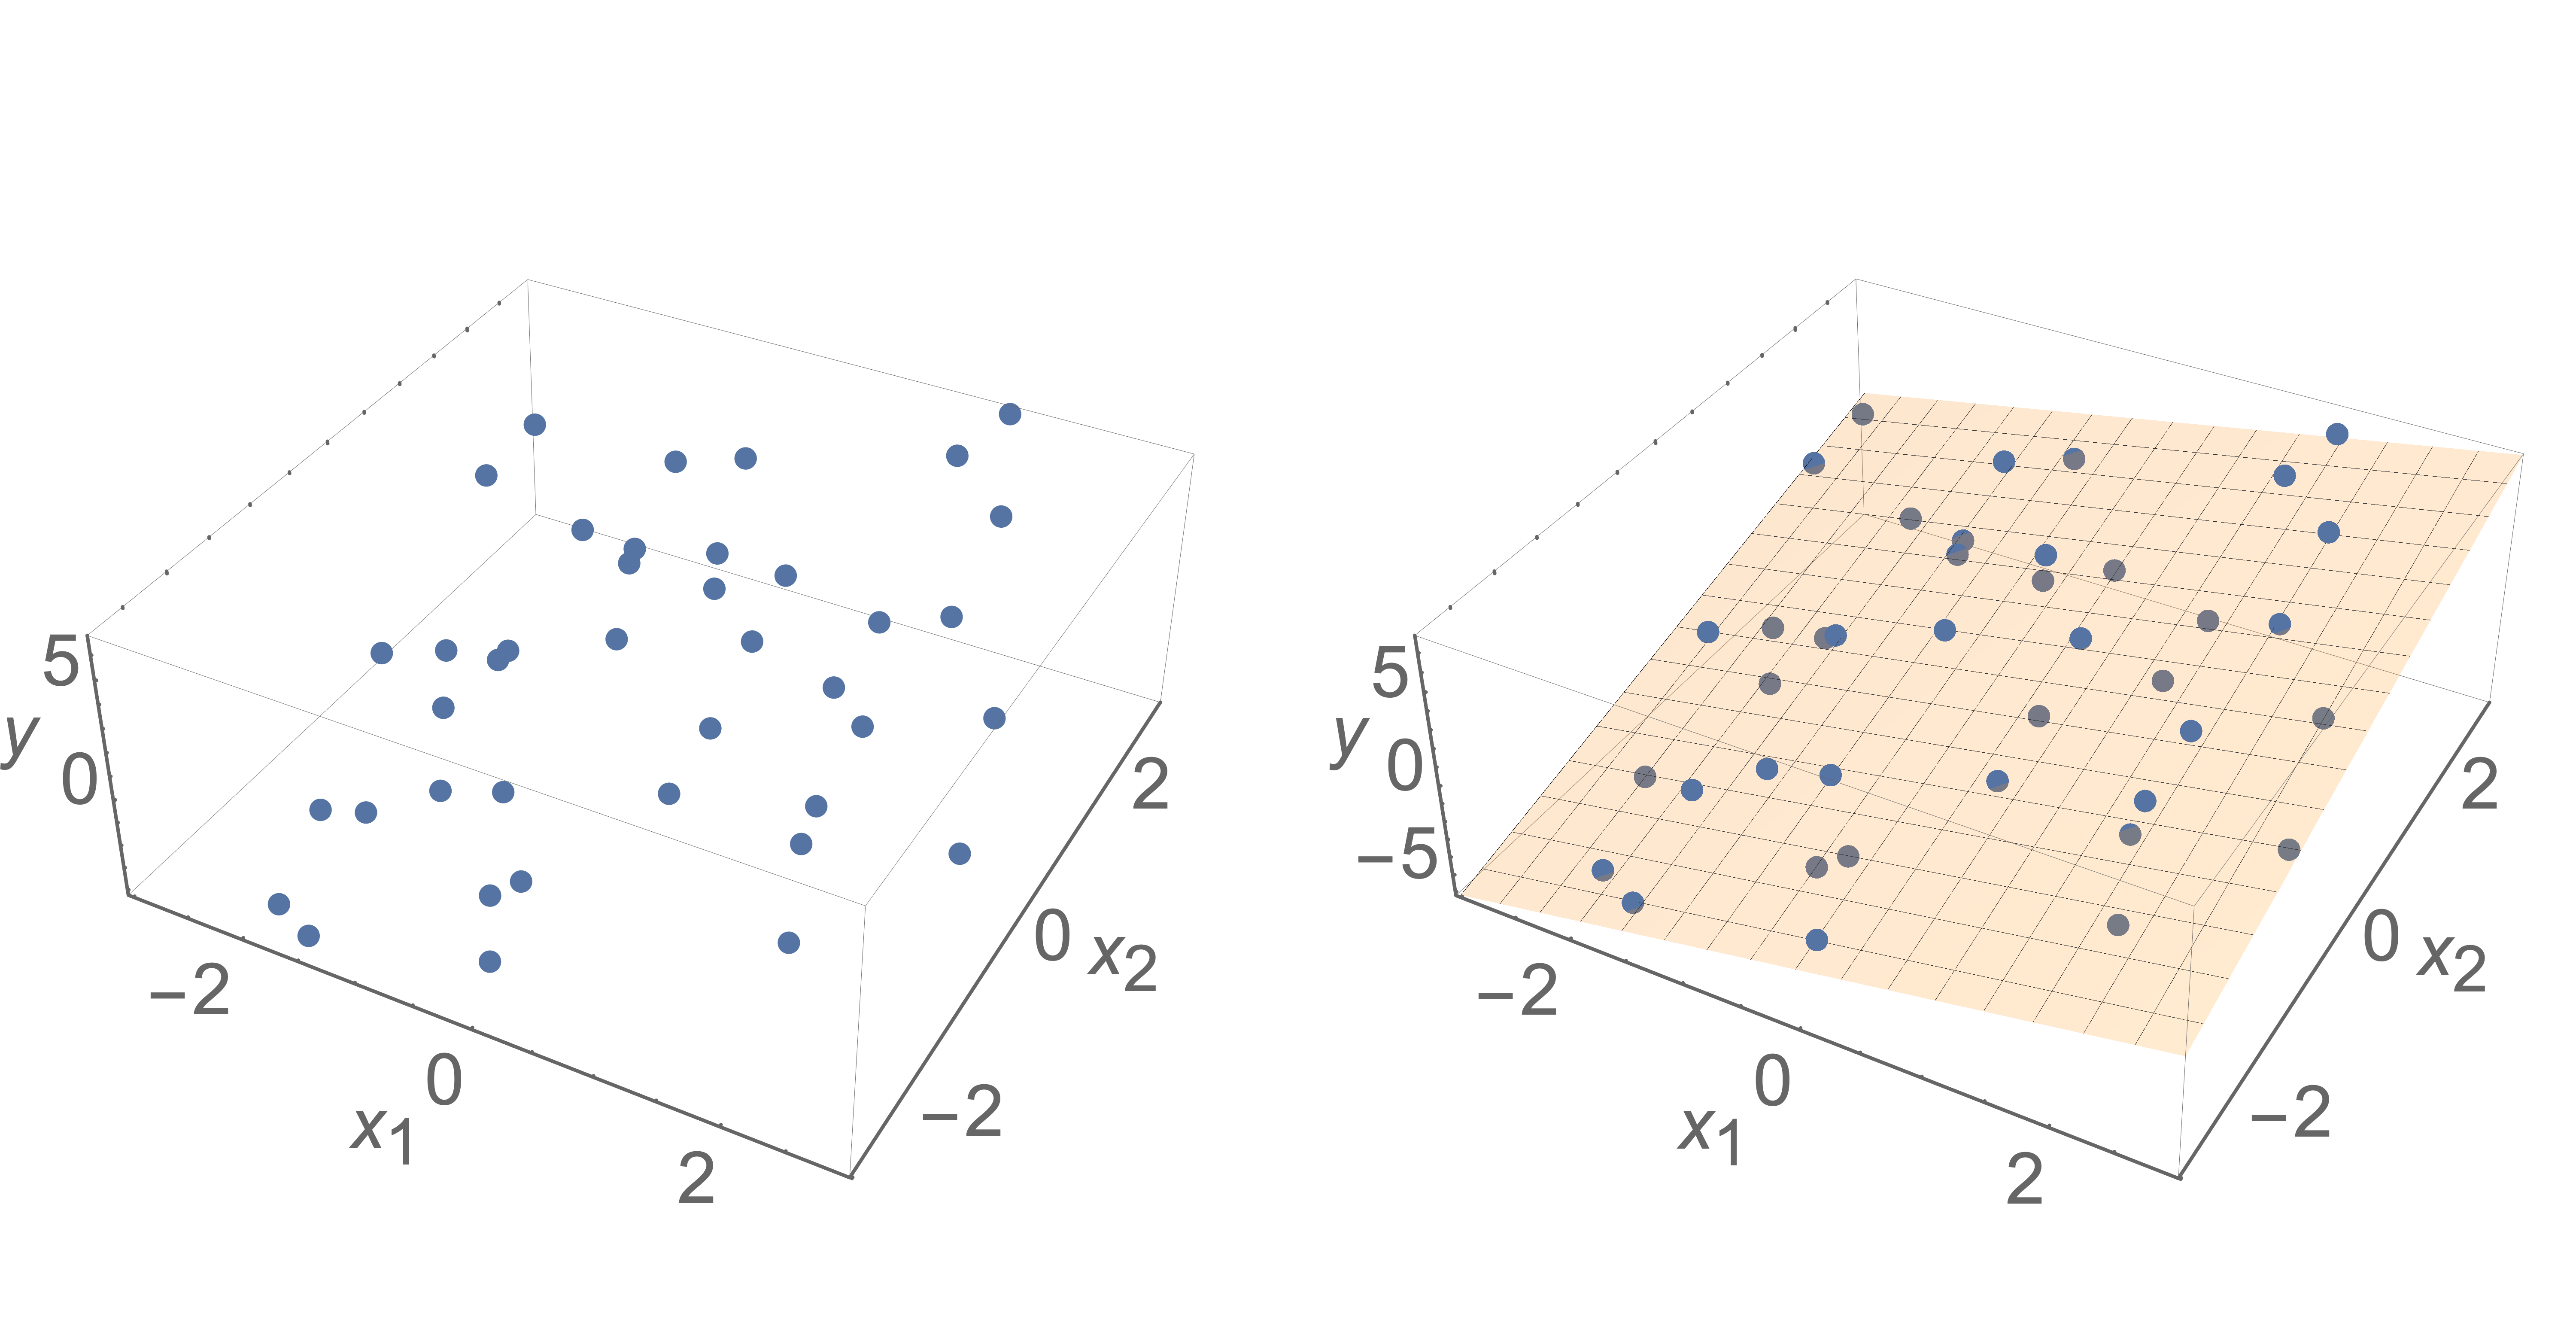
\includegraphics[width=0.9\textwidth]{figures/regression_ex1_plane1.png}

A richer class of hypotheses can be obtained by performing a
non-linear feature transformation before doing the regression, as
we will later see (in Chapter~\ref{chap-features}), but it will still
end up that we have to solve a linear regression problem.

% Here, we begin with the foundations, studying {\em linear} regression, including
% its framing as an optimization problem (Section~\ref{sec-reg_optim}),
% how to use {\em regularization} to keep solutions generalizable
% (Section~\ref{sec-regularization}), and how to evaluate {\em
%   learning algorithms} which solve the regression problem
% (Section~\ref{sec-reg_learn_alg}).


\section{A gloriously simple linear regression algorithm}

Okay!  Given the objective in Eq.~\ref{eq:reg_mse_withconst}, how
can we find good values of $\theta$ and $\theta_0$?  We'll study
several general-purpose, efficient, interesting algorithms.  But
before we do that, let's start with the simplest one we can think of:
{\em guess a whole bunch ($k$) of different values of $\theta$ and
$\theta_0$}, see which one has the smallest error on the training
set, and return it.

\begin{codebox}
  \Procname{$\proc{Random-Regression}(\data, k)$}
  \li For $i$ in  $1\dots k$: Randomly generate hypothesis $\ex{\theta}{i},
    \ex{\theta_0}{i}$
  \li Let $i = \argmin{i} J(\ex{\theta}{i}, \ex{\theta_0}{i}; \data)$
  \li Return $\ex{\theta}{i}, \ex{\theta_0}{i}$
\end{codebox}

This seems kind of silly, but it's a learning algorithm, and it's not
completely useless. \index{regression!random regression}
\question{If your data set has $n$ data points, and the dimension of the
  $x$ values is $d$, what is the size of an individual $\ex{\theta}{i}$?}
\question{How do you think increasing the number of guesses $k$ will change the training
  error of the resulting hypothesis?}


%%%%%%%%%%%%%%%%%%%%%%%%%%%%%%%%%%%%%%%%
\section{Analytical solution: ordinary least squares}

One very interesting aspect of the problem of finding a linear hypothesis
that minimizes mean squared error is that we can find a
closed-form formula for the answer!\note{What does ``closed form''
  mean?  Generally, that it involves direct evaluation of a
  mathematical expression using a fixed number of ``typical''
  operations (like arithmetic operations, trig functions, powers,
  etc.).  So equation~\ref{olsObjective} is not in closed form,
  because it's not at all clear what operations one needs to perform
  to find the solution.} This general problem is often
called the {\em ordinary least squares} ({\sc ols})

Everything is easier to deal with if we assume that all of the the $\ex{x}{i}$
have been augmented with an extra input dimension (feature) that
always has value 1, so that they are in $d+1$ dimensions, and rather
than having an explicit $\theta_0$, we let it be the last element of
our $\theta$ vector, so that we have, simply,
\[y = \theta^T x\;\;.\]
In this case, the objective becomes
\begin{equation}
  J(\theta) = \frac{1}{n}\sum_{i =
    1}^n\left(\theta^Tx^{(i)} - \ex{y}{i}\right)^2 \;\;.
  \label{eq:reg_mse}
\end{equation}

\question{
  Stop and prove to yourself that adding that extra feature
  with value 1 to every input vector and getting rid of the $\theta_0$
  parameter is equivalent to our original model.
}

We approach this just like a minimization problem from calculus
homework:  take the derivative of $J$ with respect to $\theta$, set it
to zero, and solve for $\theta$.  There are additional steps
required, to check that the resulting $\theta$ is a minimum (rather
than a maximum or an inflection point) but we won't work through that
here.   It is possible to approach this problem by:
\begin{itemize}
  \item Finding $\partial{J}/\partial{\theta_k}$ for $k$ in
        \anchorednote{$1, \ldots, d$,}{We will use $d$ here for the total number of features in
          each $\ex{x}{i}$, including the added 1.}
  \item Constructing a set of $k$ equations of the form
        $\partial{J}/\partial{\theta_k} = 0$, and
  \item Solving the system for values of $\theta_k$.
\end{itemize}
That works just fine.  To get practice for applying techniques like
this to more complex problems, we will work through a more compact
(and cool!) matrix view. Along the way, it will be helpful to collect all of the derivatives in one
vector. In particular,
the
gradient of $J$ with respect to $\theta$ is following column vector of length $d$:
\[
  \nabla_\theta J =
  \begin{bmatrix}
    \partial J / \partial \theta_1 \\
    \vdots                         \\
    \partial J / \partial \theta_d
  \end{bmatrix}.
\]

\question{Work through the next steps and check your answer against ours below.}

We can think of our training data in terms of matrices $X$ and $Y$,
where each column of $X$ is an example, and each ``column'' of $Y$ is
the corresponding target output value:
\begin{equation*}
  X = \begin{bmatrix}x_1^{(1)} & \dots & x_1^{(n)} \\\vdots & \ddots &
               \vdots                        \\x_d^{(1)} & \dots & x_d^{(n)}\end{bmatrix} \;\;\;
  Y = \begin{bmatrix}y^{(1)} & \dots & y^{(n)}\end{bmatrix}\;\;.
\end{equation*}
\question{
  What are the dimensions of $X$ and $Y$?
}


In most textbooks, they think of an individual example $\ex{x}{i}$ as
a row, rather than a column.  So that we get an answer that will be
recognizable to you, we are going to define a new matrix and vector,
% $W$ and $T$, which are just transposes of our $X$ and $Y$, and
$\Xt$ and $\Yt$, which are just transposes of our $X$ and $Y$, and
then work with them:
$$ \Xt = X^T = \begin{bmatrix}x_1^{(1)} & \dots & x_d^{(1)}\\\vdots & \ddots & \vdots\\x_1^{(n)} & \dots & x_d^{(n)}\end{bmatrix} \;\;
  \Yt = Y^T = \begin{bmatrix}y^{(1)}\\\vdots\\y^{(n)}\end{bmatrix} \;\;.$$
\question{
  What are the dimensions of $\Xt$ and $\Yt$?
}

Now we can write
\[ J(\theta) = \frac{1}{n}\underbrace{(\Xt\theta - \Yt)^T}_{1 \times
    n}\underbrace{(\Xt\theta - \Yt)}_{n \times 1} =
  \frac{1}{n}\sum_{i=1}^n \left(\left(\sum_{j=1}^d \Xt_{ij}\theta_j
    \right) - \Yt_i\right)^2\]
and using facts about matrix/vector calculus, we get \note{You should
  be able to verify this by doing a simple (say, $2 \times 2$) example by hand.}
\begin{equation}
  \nabla_{\theta}J = \frac{2}{n}\underbrace{\Xt^T}_{d \times n}\underbrace{(\Xt\theta - \Yt)}_{n \times 1}\;\;.
  % \label{eq:reg_gd_deriv}
\end{equation}
See Appendix~\ref{app:matrix_deriv} for a nice way to think about finding this
derivative.

Setting $ \nabla_{\theta}J$ to 0 and solving, we get:
\begin{align*}
  \frac{2}{n}\Xt^T(\Xt\theta - \Yt) & = 0                          \\
  \Xt^T\Xt\theta - \Xt^T \Yt        & = 0                          \\
  \Xt^T\Xt\theta                    & =  \Xt^T \Yt                 \\
  \theta                            & =  (\Xt^T\Xt)^{-1} \Xt^T \Yt \\
\end{align*}
And the dimensions work out!
$$ \theta = \underbrace{\left(\Xt^T\Xt\right)^{-1}}_{d \times d}\underbrace{\Xt^T}_{d \times n}\underbrace{\Yt}_{n \times 1} $$
So, given our data, we can directly compute the linear regression that
minimizes mean squared error.  That's pretty awesome!

%%%%%%%%%%%%%%%%%%%%%%%%%%%%%%%%%%%%%%%%%%%%%%%%%%%%%%%%%%%%%%%%%%%%%%%%%%%%%
\section{Regularization}

\label{sec-regularization}

The objective function of Eq.~\ref{eq:ml_objective_loss} balances
(training-data) memorization, induced by the {\em loss} term, with generalization,
induced by the {\em regularization} term.  Here, we address the need
for regularization specifically for linear regression, and show how
this can be realized using one popular regularization technique called {\em ridge regression}.

%%%%%%%%%%%%%%%%%%%%%%%%%%%%%%%%%%%%%%%%
\subsection{Regularization and linear regression}

If all we cared about was finding a hypothesis with small loss on the
training data, we would have no need for regularization, and could
simply omit the second term in the objective.  But remember that our
ultimate goal is to {\em perform well on input values that we haven't
    trained on!}  It may seem that this is an impossible task, but
humans and machine-learning methods do this successfully all the
time.  What allows {\em generalization} to new input values is a
belief that there is an underlying regularity that governs both the
training and testing data.  One way to
describe an assumption about such a regularity is by choosing a
limited class of possible hypotheses.  Another way to do this is to
provide smoother guidance, saying that, within a hypothesis class, we
prefer some hypotheses to others.  The regularizer articulates this
preference and the constant $\lambda$ says how much we are willing to
trade off loss on the training data versus preference over hypotheses.

%%%%%%%%%%%%%%%%%%%%%%%%%%%%%%%%%%%%%%%%
\begin{comment}
This trade-off is illustrated in the figure below.  Hypothesis $h_1$
has zero training loss, but is very complicated.  Hypothesis $h_2$
mis-classifies two points, but is very simple.  In absence of other
beliefs about the solution, it is often better to prefer that the
solution be ``simpler,'' and so we might prefer $h_2$ over $h_1$,
expecting it to perform better on future examples drawn from this same
distribution.  \note{To establish some vocabulary, we say that
  $h_1$ is {\em overfit} to the training data.}  Another nice way of
thinking about regularization is that we would like to prevent our
hypothesis from being too dependent on the particular training data
that we were given: we would like for it to be the case that if the
training data were changed slightly, the hypothesis would not change
by much.

\begin{center}
  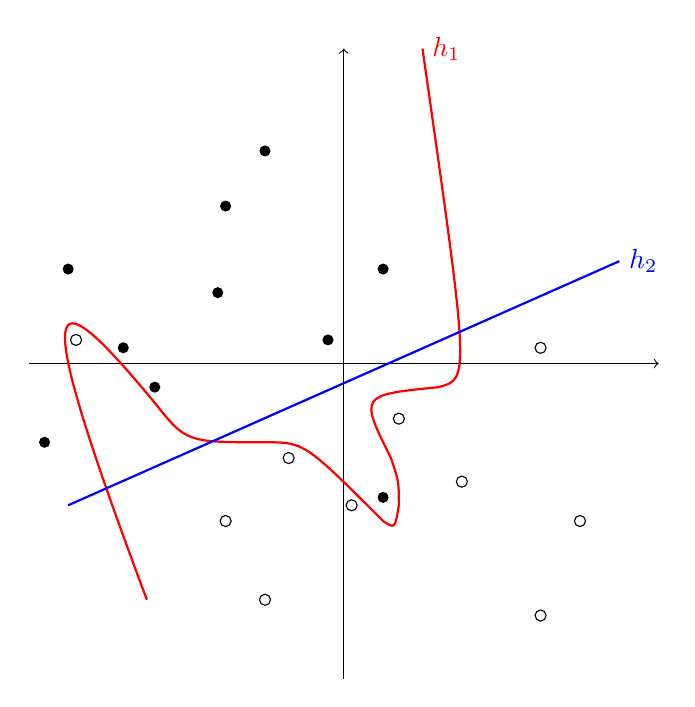
\begin{tikzpicture}
    \draw [->] (-4,0) -- (4,0);
    \draw [->] (0,-4) -- (0,4);
    \draw[red,thick] (-2.5,-3) .. controls (-4,1) and (-3.8,1.2) .. (-2.4,-.5)
    .. controls (-2,-1) .. (-1,-1) .. controls (-.5,-1) ..  (.5,-2)
    .. controls (.65, -2.1) .. (.7,-1.8) .. controls (.7,-1.5)
    ..  (.6,-1.2) .. controls (.2,-.4) .. (1.2, -.3)
    .. controls (1.6,-.2) .. (1,4);

    \foreach \Point in {(-3.4, .3), (2.5, .2), (-1.5,-2), (-1,-3),(.7,-.7),
        (3, -2), (2.5, -3.2), (-.7,-1.2), (0.1,-1.8), (1.5, -1.5)}{
        \draw \Point circle[radius=2pt];
      }
    \foreach \Point in {(.5,-1.7),(-.2,.3),(-2.8,.2),(-2.4,-.3),(-1,2.7),
        (-1.5, 2), (-1.6, .9), (-3.8,-1), (-3.5,1.2),(.5, 1.2)}{
        \fill \Point circle[radius=2pt];
      }
    \draw[blue, thick] (-3.5,-1.8) -- (3.5,1.3);
    \node[right,blue] at (3.5,1.3) {$h_2$};
    \node[below,right,red] at (1,4) {$h_1$};

  \end{tikzpicture}
\end{center}
\end{comment}
%%%%%%%%%%%%%%%%%%%%%%%%%%%%%%%%%%%%%%%%

For example, consider what happens when $d=2,$ and $x_2$ is highly
correlated with $x_1$, meaning that the data look like a line, as
shown in the left panel of the figure below.  Thus, there isn't a unique best hyperplane.\note{Sometimes there's technically a
  unique best hyperplane, but just because of noise.}  Such
correlations happen often in real-life data, because of underlying
common causes; for example, across a population, the height of people
may depend on both age and amount of food intake in the same way.
This is especially the case when there are many feature dimensions
used in the regression.  Mathematically, this leads to $\Xt^T\Xt$
close to singularity, such that $(\Xt^T\Xt)^{-1}$ is undefined or has huge
values, resulting in unstable models (see the middle panel of figure
and note the range of the $y$ values---the slope is huge!):

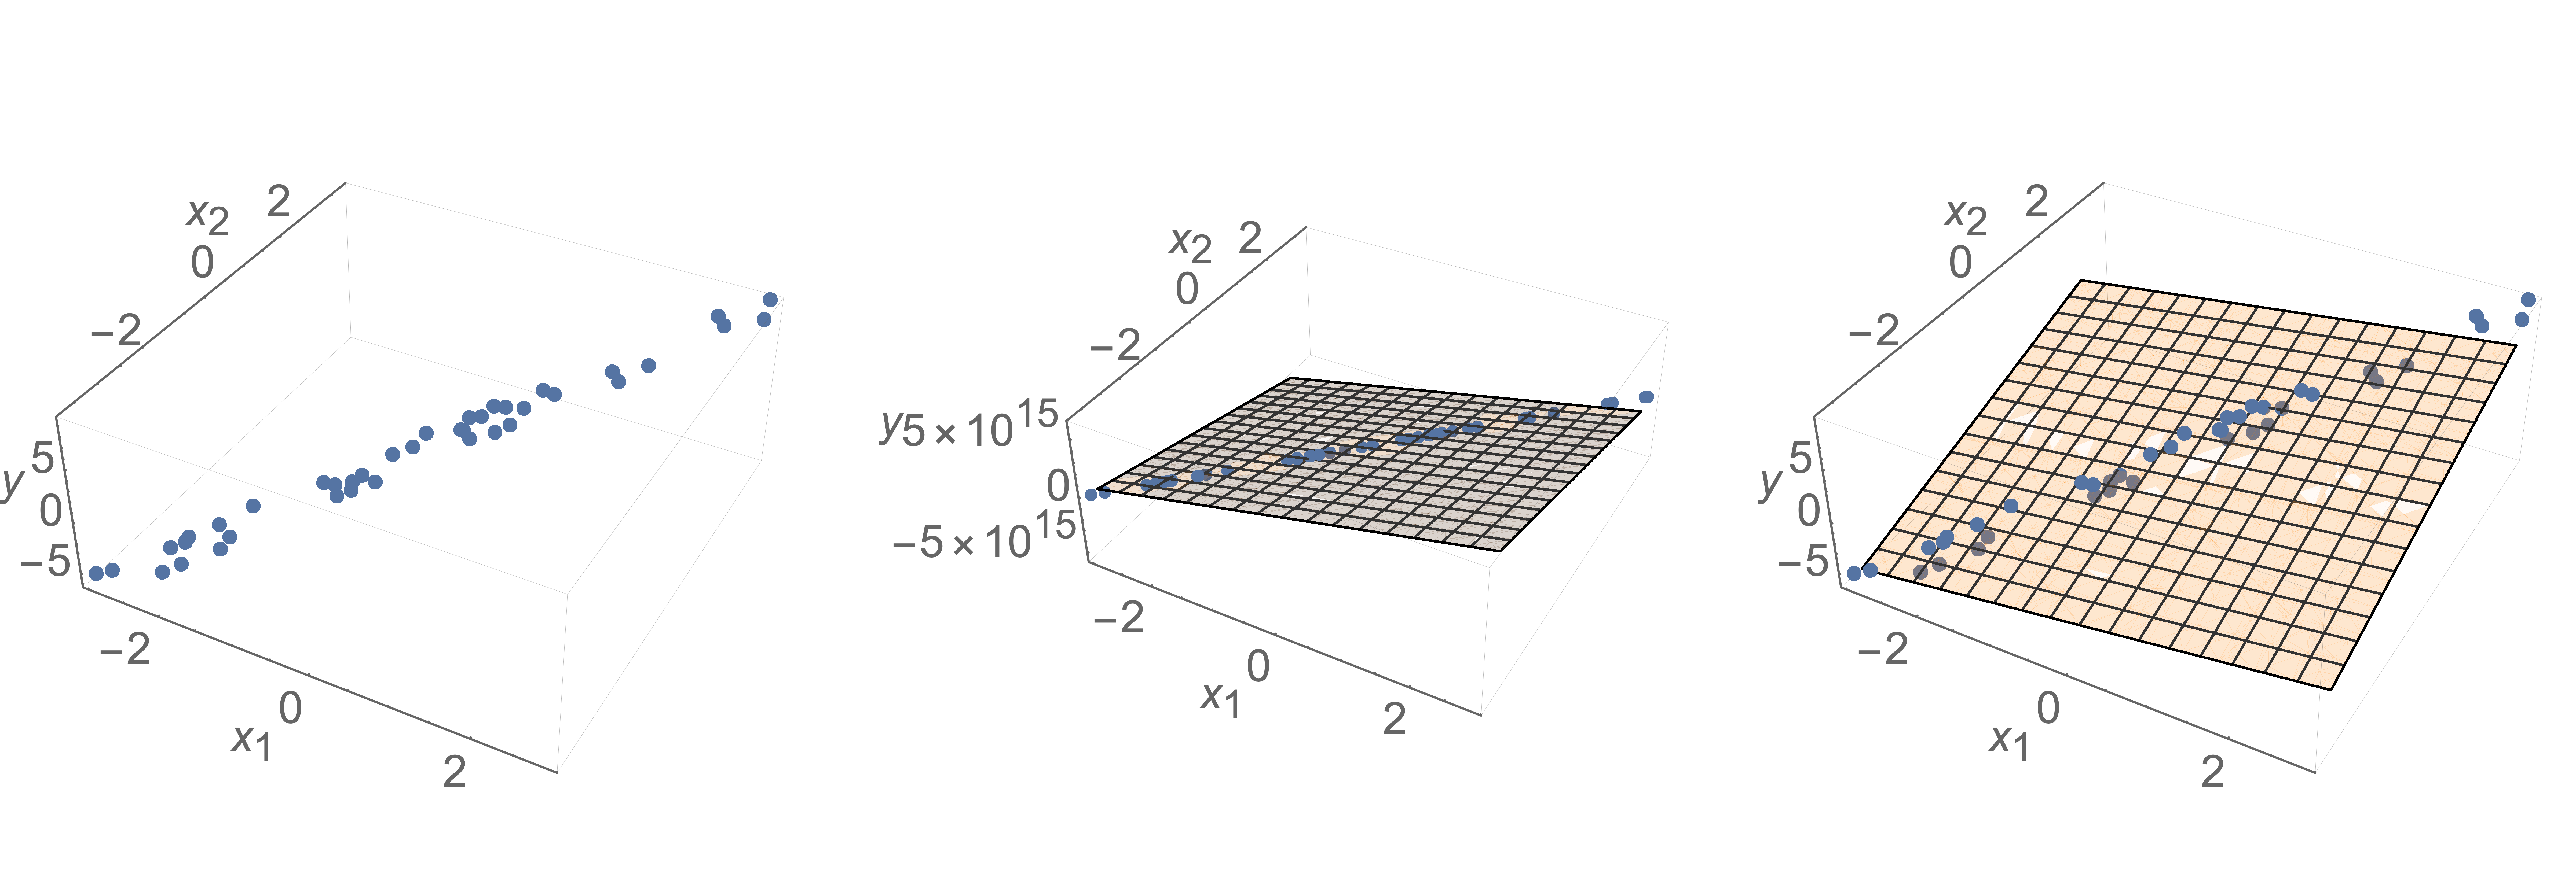
\includegraphics[width=1.12\textwidth]{figures/regression_ex2_plane1.png}

% (* mathematica: effect of regularization *)
% npts = 40;
% SeedRandom[3];
% x1 = RandomReal[{-3, 3}, {npts}];
% x2 = 1.2 * x1 + 0.3;
% noise = RandomReal[{-1.5, 1.5}, {npts}];
% yv = x1 + 1.4 * x2 + 1 + noise;
% pts = Transpose@{x1, x2, yv};
%
% regmodel =
%  Fit[pts, {1, Subscript[x, 1], Subscript[x, 2]}, {Subscript[x, 1],
%    Subscript[x, 2]}, FitRegularization -> {Tikhonov, 0.1}]
%
% model =
%  LinearModelFit[
%   pts, { Subscript[x, 1], Subscript[x, 2]}, { Subscript[x, 1],
%    Subscript[x, 2]}]
%
% p1 = ListPointPlot3D[ pts,
%    AxesLabel -> {Subscript[x, 1], Subscript[x, 2], y} ];
% p2 = ListPlot3D[ pts ];
% p3 = Plot3D[
%    model[Subscript[x, 1], Subscript[x, 2]], {Subscript[x, 1], -3,
%     3}, {Subscript[x, 2], -3, 3}, PlotStyle -> Opacity[0.2]
%    ];
% p5 = Plot3D[
%    regmodel, {Subscript[x, 1], -3, 3}, {Subscript[x, 2], -3, 3},
%    PlotStyle -> Opacity[0.2]];
% p4 = Show[{p1, p3}];
% p6 = Show[{p1, p5}];
% gr1 = GraphicsRow[{p1, p4, p6}, ImageSize -> Large]
% Export["regression_ex2_plane1.png", gr1, ImageResolution -> 1200]

A common strategy for specifying a \emph{regularizer} is to use the form
\[ R(\Theta) = \norm{\Theta - \Theta_{\it prior}}^2 \]
when we have some idea in advance that $\Theta$ ought to be near some
value $\Theta_{\it prior}$.%
\note{Learn about Bayesian methods in machine learning to see the theory behind this and cool results!}

Here, the notion of distance is quantified by squaring the $l_2$ \textit{norm} of
the parameter vector: for any $d$-dimensional vector $v \in \mathbb{R}^d,$ the $l_2$ \textit{norm} of $v$ is defined as,
\[\|v\| = \sqrt{\sum_{i=1}^d |v_i|^2}\;\;. \]
In the absence of such knowledge a default is
to {\em regularize toward zero}:
\[ R(\Theta) = \norm{\Theta}^2\;\;. \]
%
When this is done in the example depicted above, the regression model
becomes stable, producing the result shown in the right-hand panel in
the figure.  Now the slope is much more sensible.


%%%%%%%%%%%%%%%%%%%%%%%%%%%%%%%%%%%%%%%%
\subsection{Ridge regression}

\label{sec-ridge_regression}

There are some kinds of trouble we can get into in regression problems.
What if $\left(\Xt^T\Xt\right)$ is not invertible?
\question{Consider, for example, a situation where the data-set is
just the same point repeated twice:
$\ex{x}{1} = \ex{x}{2} = [1~~2]^T$.
What is $\Xt$ in this case?  What is $\Xt^T\Xt$?  What is $(\Xt^T\Xt)^{-1}$?
}

Another kind of problem is {\em overfitting}: we have formulated an
objective that is just about fitting the data as well as possible, but
we might also
want to {\em regularize} to keep the hypothesis from getting {\em too}
attached to the data.

We address both the problem of not being able to invert $(\Xt^T\Xt)^{-1}$ and
the problem of overfitting using a mechanism called {\em ridge
    regression}.  We add a regularization term $\|\theta\|^2$ to the
  {\sc ols} objective, with a non-negative scalar value $\lambda$ to control the tradeoff
between the training error and the regularization term.
\question{Why do we emphasize the non-negativity of the scalar $\lambda?$ When we add a regularizer of the form $\|\theta\|^2$, what
  is our most ``preferred'' value of $\theta$, in the absence of any
  data?}
Here is the ridge regression objective function:\index{regression!ridge regression}
$$ J_{\text{ridge}}(\theta, \theta_0) = \frac{1}{n}\sum_{i = 1}^n\left(\theta^Tx^{(i)} + \theta_0 - y^{(i)}\right)^2 + \lambda\|\theta\|^2 $$
Larger $\lambda$ values pressure $\theta$ values to be near zero.
Note that we don't penalize $\theta_0$; intuitively, $\theta_0$ is
what ``floats'' the regression surface to the right level for the data
you have, and so you shouldn't make it harder to fit a data set where
the $y$ values tend to be around one million than one where they tend
to be around one.  The other parameters control the orientation of the
regression surface, and we prefer it to have a not-too-crazy
orientation.

There is an analytical expression for the $\theta, \theta_0$ values
that minimize $J_\text{ridge}$, but it's a little bit more complicated
to derive than the solution for {\sc ols} because $\theta_0$ needs
special treatment.   If we decide not to treat $\theta_0$ specially
(so we add a 1 feature to our input vectors as discussed above), then we get:
$$ \nabla_{\theta}J_\text{ridge} = \frac{2}{n}\Xt^T(\Xt\theta - \Yt) + 2
  \lambda \theta\;\;.$$

Setting to 0 and solving, we get:\note{Remember that $I$ stands for
  the identity matrix, a square matrix that has 1's along the diagonal and 0's
  everywhere else.}
\begin{align*}
  \frac{2}{n}\Xt^T(\Xt\theta - \Yt) + 2 \lambda \theta             & = 0                                      \\
  \frac{1}{n}\Xt^T\Xt\theta - \frac{1}{n}\Xt^T\Yt + \lambda \theta & = 0                                      \\
  \frac{1}{n}\Xt^T\Xt\theta  + \lambda \theta                      & = \frac{1}{n}\Xt^T\Yt                    \\
  \Xt^T\Xt\theta  + n \lambda \theta                               & = \Xt^T\Yt                               \\
  (\Xt^T\Xt  + n \lambda I)\theta                                  & = \Xt^T\Yt                               \\
  \theta                                                           & = (\Xt^T\Xt  + n \lambda I)^{-1}\Xt^T\Yt
\end{align*}
Whew!  So the solution is:
\begin{equation}
  \theta_{\text{ridge}} = \left(\Xt^T\Xt + n\lambda I\right)^{-1}\Xt^T\Yt
  \label{eq:ridge_regression_solution}
\end{equation}

Now, why is the term $\left(\Xt^T\Xt + n\lambda I\right)$\note{This is called 
``ridge'' regression because we are adding a ``ridge'' of $n\lambda$ 
values along the diagonal of the matrix before inverting it.} invertible? 
Explaining this requires some linear algebra. The matrix $\Xt^T\Xt$ is positive 
semidefinite, which implies that its eigenvalues $\{\gamma_i\}_i$ are greater
than or equal to 0. The matrix $\Xt^T\Xt+n\lambda I$ has eigenvalues 
$\{\gamma_i+n\lambda\}_i$ which are guaranteed to be strictly positive since
$\lambda>0$. Recalling that the determinant of a matrix is simply the product of its eigenvalues, 
we get that $\det(\Xt^T\Xt + n\lambda I)>0$ and conclude that $\Xt^T\Xt + n\lambda I$ is invertible.

\question{Why is $\Xt^T\Xt$ positive semidefinite?}
\question{What is the dimension of $I$ in the equation above?}



%%%%%%%%%%%%%%%%%%%%%%%%%%%%%%%%%%%%%%%%%%%%%%%%%%%%%%%%%%%%%%%%%%%%%%%%%%%%%
\section{Evaluating learning algorithms}\label{sec-reg_learn_alg}

In this section, we will explore how to evaluate supervised
machine-learning algorithms.  We will study the special case of
applying them to regression problems, but the basic ideas of
validation, hyper-parameter selection, and cross-validation apply much
more
broadly.

We have seen how linear regression is a well-formed optimization
problem, which has an analytical solution when ridge regularization is
applied.  But how can one choose the best amount of regularization, as
parameterized by $\lambda$?  Two key ideas involve the evaluation of
the performance of a hypothesis, and a separate evaluation of the
algorithm used to produce hypotheses, as described below.

%%%%%%%%%%%%%%%%%%%%%%%%%%%%%%%%%%%%%%%%
\subsection{Evaluating hypotheses}

The performance of a given hypothesis $h$ may be evaluated by
measuring {\em test error} on data that was not used to train it.\note{It's a bit funny to interpret the analytical
  formulas given above for $\theta$ as ``training,'' but later when we employ more statistical methods, ``training'' will be a meaningful concept.}
%
Given a training set $\data_n,$ a regression hypothesis $h$, and if we choose squared loss, we can define the OLS {\em{training error}} of $h$ to be the mean square error between its predictions and the expected outputs:
\begin{eqnarray*}
  \trainerr(h) = \frac{1}{n}\sum_{i = 1}^{n} \left[ h(\ex{x}{i}) - \ex{y}{i} \right]^2
  \;\;.
\end{eqnarray*}
Test error captures the performance of $h$ on unseen data, and is the
mean square error on the test set, with a nearly identical expression
as that above, differing only in the range of index $i$:
\begin{eqnarray*}
  \mathcal{E}(h) = \frac{1}{n'}\sum_{i = n + 1}^{n + n'} \left[ h(x^{(i)}) - y^{(i)} \right]^2
\end{eqnarray*}
on $n'$ new examples that were not used in the process of constructing $h$.

In machine learning in general, not just regression, it is useful to
distinguish two ways in which a hypothesis $h \in \hclass$ might
contribute to test error. Two are:
\begin{description}
  \item{\bf Structural error}: This is error that arises because there
        is no hypothesis $h \in \hclass$ that will perform well on the data,
        for example because the data was really generated by a sine wave but
        we are trying to fit it with a line.\index{structural error}
  \item{\bf Estimation  error}:  This is error that arises because we
        do not have enough data (or the data are in some way unhelpful) to
        allow us to choose a good $h \in \hclass$, or because we didn't
        solve the optimization problem well enough to find the best $h$
        given the data that we had.\index{estimation error}
\end{description}

\note{There are technical definitions of these concepts that are
  studied in more advanced treatments of machine learning.  Structural
  error is referred to as {\em bias} and estimation error is referred
  to as {\em variance}.}
When we increase $\lambda$, we tend to increase structural error  but
decrease estimation error, and vice versa.

% \question{
% Consider using a polynomial basis of order $k$ as a feature
% transformation $\phi$ on your data.  Would increasing $k$ tend to
% increase or decrease structural error?  What about estimation error?
% }

%%%%%%%%%%%%%%%%%%%%%%%%%%%%%%%%%%%%%%%%
\subsection{Evaluating learning algorithms}

{\em Note that this section is relevant to learning algorithms
  generally---we are just introducing the topic here since we now have
  an algorithm that can be evaluated!}

\vskip0.2in

A {\em learning algorithm}\index{learning algorithm} is a procedure that takes a data set
$\data_n$ as input and returns an hypothesis $h$ from a hypothesis
class $\hclass$; it looks like
\begin{equation*}
  \data_n \longrightarrow \boxed{\text{learning alg ($\hclass$)}} \longrightarrow h
\end{equation*}
%
% $\theta$ and $\theta_{0}$.
Keep in mind that $h$ has parameters. The learning algorithm itself may have its own parameters, and such
parameters are often called {\em hyperparameters}.  The analytical
solutions presented above for linear regression,
e.g., Eq.~\ref{eq:ridge_regression_solution}, may be thought of as
learning algorithms, where $\lambda$ is a hyperparameter that governs
how the learning algorithm works and can strongly affect its performance.

How should we evaluate the performance of a {learning algorithm}?
This can be tricky.  There are many potential sources of variability in
the possible result of computing test error on a learned hypothesis $h$:
\begin{itemize}
  \item Which particular {\em training examples} occurred in $\dataTrain$
  \item Which particular {\em testing examples} occurred in $\dataTest$
  \item Randomization inside the learning {\em algorithm} itself
\end{itemize}

\subsubsection{Validation}
Generally, to evaluate how well a learning {\em algorithm} works,
given an unlimited data source,
we would like to execute the following process multiple
times:
\begin{itemize}
  \item Train on a new training set (subset of our big data source)
  \item Evaluate resulting $h$ on a {\em validation set} that does not
        overlap the training set (but is still a subset of our same big
        data source)
\end{itemize}
% Average the performance of the resulting hypotheses over the different
% ``trials'' of training and validation.

Running the algorithm multiple times controls for possible poor choices of
training set or unfortunate randomization inside the algorithm itself.

\subsubsection{Cross validation}
\label{cross-validation}
One concern is that we might need a lot of data to do this, and in
many applications data is expensive or difficult to acquire. We can
re-use data with {\em{cross validation}}\index{cross validation} (but it's harder to do theoretical
analysis).  \\
\begin{codebox}
  \Procname{$\proc{Cross-Validate}(\data, k)$}
  \li divide $\data$ into $k$ chunks $\data_1, \data_2, \ldots \data_k$ (of roughly equal size)
  \li \For $i \gets 1$ \To $k$
  \li   \Do
  train $h_i$ on $\data \setminus \data_i$ (withholding chunk $\data_i$ as the validation set)
  \li     compute ``test'' error $\mathcal{E}_i (h_i)$ on withheld data $\data_i$
  \End
  \li \Return $\frac{1}{k} \sum_{i=1}^k \mathcal{E}_i (h_i)$
\end{codebox}

It's very important to understand that (cross-)validation neither
delivers nor evaluates a single particular hypothesis $h$.  It
evaluates the {\em learning algorithm} that produces hypotheses.

\subsubsection{Hyperparameter tuning}
The hyper-parameters of a learning algorithm affect how the algorithm
  {\em works} but they are not part of the resulting hypothesis.  So,
for example, $\lambda$ in ridge regression affects {\em which}
hypothesis will be returned, but $\lambda$ itself doesn't show up in
the hypothesis (the hypothesis is specified using parameters $\theta$ and
$\theta_0$).

You can think about each different setting of a hyper-parameter as
specifying a different learning algorithm.

In order to pick a good value of the hyper-parameter, we often end up
just trying a lot of values and seeing which one works best via
validation or cross-validation.\index{hyperparameter!hyperparameter tuning}


\question{How could you use cross-validation to decide whether to use
  analytic ridge regression or our random-regression algorithm and to pick
  $K$ for random regression or $\lambda$ for ridge regression?}



%%% Local Variables:
%%% mode: latex
%%% TeX-master: "top"
%%% End:

\chapter{Gradient Descent}
\label{chap-gradient}
\vspace*{-0.1in}
In the previous chapter,
we showed how to describe an interesting objective function for
machine learning, but we need a way to
find the optimal $\Theta^* = \argmin{\Theta} J(\Theta)$, particularly
when the objective function is not amenable to analytical
optimization.  For example, this can be the case when $J(\Theta)$
involves a more complex loss function, or more general forms of
regularization.  It can also be the case when there is simply too much
data for it to be computationally feasible to analytically invert the
required matrices.

There is an
enormous and fascinating literature on the mathematical and algorithmic
foundations of optimization\note{Which you should consider studying
  some day!}, but for this class, we will consider one of the simplest
methods, called {\em gradient descent.}

Intuitively, in one or two dimensions, we can easily think of
$J(\Theta)$ as defining a surface over $\Theta$;  that same idea
extends to higher dimensions.  Now, our objective is to find the
$\Theta$ value at the lowest point on that surface.  One way to think
about gradient descent is that you start at some arbitrary point on
the surface, look to see in which direction the ``hill'' goes down
most steeply, take a small step in that direction, determine the
direction of steepest descent from where you are, take another small
step, etc.

Below, we explicitly give gradient descent algorithms for one and
multidimensional objective functions (Sections~\ref{sec-gd_onedim}
and~\ref{sec-gd}).  We then illustrate the application of gradient
descent to a loss function which is not merely mean squared loss
(Section~\ref{sec-gd_ridge}).  And we present an important method known
as {\em stochastic gradient descent}
(Section~\ref{sec-sgd}), which is
especially useful when datasets are too large for descent in a single
batch, and has some important behaviors of its own.

%%%%%%%%%%%%%%%%%%%%%%%%%%%%%%%%%%%%%%%%%%%%%%%%%%%%%%%%%%%%%%%%%%%%%%%%%%%%%
\section{Gradient descent in one dimension}\label{sec-gd_onedim}

We start by considering gradient descent in one dimension. Assume
$\Theta \in \R$, and that we know both $J(\Theta)$ and its first
derivative with respect to $\Theta$, $J'(\Theta)$.  Here is pseudo-code
for gradient descent on an arbitrary function $f$\index{gradient descent}.  Along with $f$ and
its gradient
% AM_S2024 begin
$\nabla_{\Theta}f$ (which, in the case of a scalar $\Theta$, is the same as its derivative $f'$),
% AM_S2024 end
we have to specify some hyper-parameters.
These hyper-parameters include the initial value for parameter $\Theta$, a {\em step-size}
hyper-parameter $\eta$, and an {\em accuracy} hyper-parameter~$\epsilon$\index{gradient descent!learning rate}.

The hyper-parameter $\eta$ is often called {\em learning rate} when
gradient descent is applied in machine learning. For simplicity, $\eta$ may be taken as a constant, as is the case in the pseudo-code below; and we'll see adaptive (non-constant) step-sizes soon. What's important to notice though, is that even when $\eta$ is constant, the actual magnitude of the
change to $\Theta$ may not be constant, as that change depends on the
magnitude of the gradient itself too.

\begin{codebox}
  \Procname{$\proc{1D-Gradient-Descent}(\Theta_{\it init}, \eta, f,
      f', \epsilon)$}
  \li $\Theta^{(0)} \gets \Theta_{\it init}$
  \li $t \gets 0$
  \li \Repeat
  \li   $t \gets t+1$
  \li   $\Theta^{(t)} = \Theta^{(t-1)} - \eta \, f'(\Theta^{(t-1)})$
  \li \Until $|f(\Theta^{(t)}) - f(\Theta^{(t-1)})| < \epsilon$
  \li \Return $\Theta^{(t)}$
\end{codebox}
Note that this algorithm terminates when the change in the function $f$
is sufficiently small. There are many other reasonable ways to decide
to terminate, including\index{gradient descent!stopping criteria}:
\begin{itemize}
  \item Stop after a fixed number of iterations $T$, i.e.,\ when $t = T$.
  \item Stop when the change in the value of the parameter
        $\Theta$ is sufficiently small, i.e.,\ when $\left| \Theta^{(t)} - \Theta^{(t-1)} \right|
          <\epsilon$.
  \item Stop when the derivative $f'$ at the latest value of $\Theta$ is sufficiently small, i.e.,\ when $\left|f'(\Theta^{(t)}) \right|
          <\epsilon$.
\end{itemize}

\question{Consider all of the potential stopping criteria for $\proc{1D-Gradient-Descent}$, both in the algorithm as it appears
  and listed separately later.
  Can you think of ways that any two of the criteria relate to each other?
}

\begin{theorem}
  Choose any small distance $\tilde{\epsilon} > 0$.
  If we assume that $f$ has a minimum, is sufficiently ``smooth'' and \anchorednote{convex,}{A function is convex if the line segment between any two points on the graph of the function lies above or on the graph.}
  and if the step size $\eta$ is sufficiently small, gradient descent will reach a point within $\tilde{\epsilon}$ of a global optimum point $\Theta$.\index{gradient descent!convergence}

  % Previous theorem:
  %  for any desired accuracy $\epsilon$, there is some
  %  step size $\eta$ such that gradient
  %  descent will converge to within $\epsilon$ of the optimal $\Theta$.
  %
  % Previous theorem has bug: doesn't quite hold for horizontal line; also,
  % it won't be epsilon away; it'll get arbitrarily close with the distances going to 0
\end{theorem}
However, we must be careful when choosing the step size to prevent
slow convergence, non-converging oscillation around the minimum, or divergence.

The following plot illustrates a convex function $f(x) = (x - 2)^2$,
starting gradient descent at $x_\textrm{init} = 4.0$ with a step-size of
$1/2$.  It is very well-behaved!

\begin{center}
  \begin{tikzpicture}
    \begin{axis}[
        axis lines=middle,
        xmin=-1, xmax=6,
        ymin=-1, ymax=5,
        xlabel={$x$}, ylabel={$f(x)$},
      ]
      \addplot [domain=-1:6, samples=100] {(x-2)^2};
      \addplot [only marks,color=black,mark=*,mark size=1.5pt] coordinates {
          (2,0)
          (4,4)};
      \draw[-latex,blue,thick] (axis cs: 4,4) -- (axis cs: 2,0);
    \end{axis}
  \end{tikzpicture}
\end{center}

\question{What happens in this example with very small $\eta$?  With
  very big $\eta$?}

If $f$ is non-convex, where gradient descent converges to depends on
$x_{\it init}$.  First, let's establish some
definitions. Suppose we have analytically defined derivatives for $f$.
Then we say that $f$ has a {\em local minimum point} or {\em local optimum point}
at $x$ if
$f'(x) = 0$ and $f''(x)
  > 0$, and we say that $f(x)$ is a {\em local minimum value} of $f$.
More generally, $x$ is a local minimum point of $f$ if $f(x)$ is at
least as low as $f(x')$ for all points $x'$ in some small area around $x$.
We say that $f$ has a {\em global
    minimum point} at $x$ if $f(x)$ is at least as low as $f(x')$ for every other input $x'$.
And then we call $f(x)$ a {\em global minimum value}.
A global minimum point is also a local minimum point, but a local
minimum point does not have to be a global minimum point.

If $f$ is non-convex (and sufficiently smooth),
% AM_S2024 begin
one expects that
% AM_S2024 end
gradient descent (run long enough with small enough step size) will get very close to a point at which the gradient is zero, though
we cannot guarantee that it will converge to a global minimum point.
% \note{There are many "gaps" between a point having zero gradient and a global minimum. For example, a local maximum, or a so-called saddle point would be a point at which gradient is zero.}

% AM_S2024 begin
There are two notable exceptions to this common sense expectation: First, gradient descent can get stagnated while approaching a point $x$ which is not a local minimum or maximum,
but satisfies $f'(x)=0$. For example, for $f(x)=x^3$, starting gradient descent from the
initial guess $x_{\it init}=1$, while using step size $\eta<1/3$
will lead to $x^{(k)}$ converging to zero as $k\to\infty$. Second, there are functions (even convex ones) with no minimum points,
like $f(x)=\exp(-x)$, for which gradient descent with a positive step size converges to $+\infty$.
% AM_S2024 end

The plot below shows two different $x_{\it init}$, and how gradient descent
started from each point heads toward two different local optimum points.
\begin{center}
  \begin{tikzpicture}
    \begin{axis}[
        axis lines=middle,
        xmin=-2, xmax=4,
        ymin=2, ymax=10,
        xlabel={$x$}, ylabel={$f(x)$},
      ]
      \addplot [domain=-2:4, samples=100] {0.5*x^4 - 3*x^3 + 4*x^2 + 3*x + 3};
      \draw[-latex,blue,thick] (axis cs: -1,7.5) -- (axis cs: -0.52,2.98);
      \draw[-latex,blue,thick] (axis cs: -.52,2.98) -- (axis cs: -0.40, 2.65);
      \draw[-latex,blue,thick] (axis cs: -0.40, 2.65) -- (axis cs: -0.28, 2.54);

      \draw[-latex,blue,thick] (axis cs: 2,9) -- (axis cs: 2.15,8.81);
      \draw[-latex,blue,thick] (axis cs: 2.15,8.81) -- (axis cs: 2.38,8.40);
      \draw[-latex,blue,thick] (axis cs: 2.38,8.40) -- (axis cs: 2.68, 7.82);
      \draw[-latex,blue,thick] (axis cs: 2.68, 7.82) -- (axis cs: 2.93, 7.52);
      \draw[-latex,blue,thick] (axis cs: 2.93, 7.52) -- (axis cs: 3, 7.5);

      \addplot [only marks,color=black,mark=*,mark size=1.5pt] coordinates {
          (-1, 7.5)
          (-.4, 2.65)
          (2, 9)
          (3, 7.5)};
    \end{axis}
  \end{tikzpicture}
\end{center}

%%%%%%%%%%%%%%%%%%%%%%%%%%%%%%%%%%%%%%%%%%%%%%%%%%%%%%%%%%%%%%%%%%%%%%%%%%%%%
\section{Multiple dimensions}
\label{sec-gd}

The extension to the case of multi-dimensional $\Theta$ is
straightforward.  Let's  assume $\Theta \in \R^m$, so $f: \R^m
  \rightarrow \R$. The
gradient of $f$ with respect to $\Theta$ is
\[
  \nabla_\Theta f =
  \begin{bmatrix}
    \partial f / \partial \Theta_1 \\
    \vdots                         \\
    \partial f / \partial \Theta_m
  \end{bmatrix}
\]
The algorithm remains the same, except that the update step in line 5
becomes
\[ \ex{\Theta}{t} = \ex{\Theta}{t-1} - \eta\nabla_\Theta f(\ex{\Theta}{t-1}) \]
and any termination criteria that depended on the dimensionality
of $\Theta$ would have to change.  The easiest thing is
to keep the test in line 6 as $\left|f(\ex{\Theta}{t}) -
  f(\ex{\Theta}{t-1}) \right| < \epsilon$, which is sensible no matter
the dimensionality of $\Theta$.
\question{Which termination criteria from the 1D case were defined in
  a way that assumes $\Theta$ is one dimensional?
}

% % AM_S2024 begin
% \subsection{Gradient vs. Derivative}
% It is easy to fall into habit of using the words {\sl gradient} and {\sl derivative} interchangeably, but there is actually a significant difference.
% For a function $f: \R^m\rightarrow \R$, its derivative at point $x\in\R^m$ (strictly speaking, its {\sl total derivative} at $x$)
% is a {\sl linear} function
% $L:\R^m\to\R$ which provides the best approximation of $f(x+\Delta)-f(x)$ for small $\Delta$,
% in the sense that
% \[
%   \lim_{\|\Delta\|\to0+}\frac{\|f(x+\Delta)-f(x)-L(\Delta)\|}{\|\Delta\|}=0.
% \]
% When the elements of $\R^m$ are viewed as
% $m$-by-1 column vectors (as we do in this class), every linear function $L:\R^m\to\R$ can be written in the form
% $L(\Delta)=p\Delta$, where $p$ is a 1-by-$m$ real row matrix, the {\sl Jacobian} of $f$ at $x$.
% This matrix $p$ is usually denoted by $p=df/dx$, and can be computed in terms of partial derivatives as
% \[
%   \frac{df}{dx}=\begin{bmatrix}
%     \partial f / \partial x_1 &
%     \dots                     &
%     \partial f / \partial x_m
%   \end{bmatrix}
% \]
% What is described above corresponds to the so-called "numerator" convention  for denoting derivatives, which is most common.


% In contrast, the {\sl gradient} $\nabla f$ of a function $f: \R^m\rightarrow \R$ at point $x\in\R^m$ provides a very rough estimate for the
% argument of maximum of $f(x+\Delta)-f(x)$ with respect to $\Delta$. The "roughness" corresponds to the fact that, instead of maximizing
% $f(x+\Delta)-f(x)$, the gradient  maximizes $L(\Delta)-0.5\|\Delta\|^2$ (equivalently, $-\nabla f$ minimizes
% $L(\Delta)+0.5\|\Delta\|^2$). Here $L(\Delta)$ is the total derivative of $f$ at
% $x$, hence a good {\sl linear} approximation of $f(x+\Delta)-f(x)$, but the $-0.5\|\Delta\|^2$ term is a wild guess at the
% second order component of the Taylor series expansion of $f(x+\Delta)-f(x)$ (to be more accurate, $-0.5\|\Delta\|^2$ should be replaced by
% $0.5\Delta^Tf''(x)\Delta$, where $f''(x)$ is the {\sl Hessian} of $f$ at $x$, but this approach is much more expensive, and has its own issues).
% When $L(\Delta)=p\Delta$, where $p$ is a 1-by-$m$ row matrix, the maximum of $L(\Delta)-0.5\|\Delta\|^2$ is achieved at $\Delta=p^T$. Hence
% the gradient is the result of transposing the matrix representation of the derivative, when one is using the "numerator" convention.

% The arbitrariness of the $\|\Delta\|^2$ term in the derivation of the gradient is glaring, which leads to the idea of replacing it with
% some other positive definite quadratic form $\Delta^TQ\Delta$, for which maximizing $L(\Delta)-0.5\Delta^TQ\Delta$ is computationally cheap (using
% $Q=f''(x)$ is very expensive in most applications, and there is the additional concern that,
% for a non-convex function, $f''(x)$ does not have to be positive definite).
% One can argue that many of the popular approaches to gradient-like optimization,
% such as the {\sl Adam} are based on using a smart selection of matrix $Q$ in an alternative definition of the gradient.

% To make things more confusing, there is an alternative "denominator" convention,
% in which the Jacobian is defined as transpose of its "numerator" version.
% The denominator convention comes naturally when one interprets the elements of $\R^m$ as {\sl row vectors}
% (i.e., 1-by-$m$ matrices), in which case linear functions
% $L:~\R^m\to\R$ are conveniently written in the form  $L(\Delta)=\Delta p$, where $p$ is a {\sl column} $m$-by-1 matrix. When the denominator
% convention is combined with treating the elements of $\R^m$ as column vectors,
% the chain rule for differentiating compositions becomes rather cumbersome.

% % AM_S2024 end


\section{Application to regression}

\label{sec-gd_ridge}

Recall from the previous chapter that choosing a loss function is the
first step in formulating a machine-learning problem as an
optimization problem, and for regression we studied the mean square
loss, which captures loss as
$({\rm guess} - {\rm actual})^2$.\index{gradient descent!applied to regression}
This leads to the {\em ordinary least squares} objective
\begin{equation}
  J(\theta) = \frac{1}{n}\sum_{i =
    1}^n\left(\theta^Tx^{(i)} - \ex{y}{i}\right)^2 \;\;.
\end{equation}
We use the gradient of the objective with respect to the parameters,
\begin{equation}
  \nabla_{\theta}J = \frac{2}{n}\underbrace{\Xt^T}_{d \times
    n}\underbrace{(\Xt\theta - \Yt)}_{n \times 1}\;\;,
  \label{eq:reg_gd_deriv}
\end{equation}
to obtain an
analytical solution to the linear regression problem.  Gradient
descent could also be applied to numerically compute a solution, using
the update rule
\begin{equation}
  \ex{\theta}{t} = \ex{\theta}{t-1} - \eta \frac{2}{n} \sum_{i=1}^{n} \left( \left[ \ex{\theta}{t-1}\right]^T x^{(i)} - y^{(i)} \right) x^{(i)}
  \,.
\end{equation}
{~\hfill ~\note{Beware double superscripts!  $\left[ \theta \right]^T$
  is the transpose of the vector $\theta$}}

\subsection{Ridge regression}
Now, let's add in the regularization term, to get the ridge-regression
objective:
$$ J_{\text{ridge}}(\theta, \theta_0) = \frac{1}{n}\sum_{i = 1}^n\left(\theta^Tx^{(i)} + \theta_0 - y^{(i)}\right)^2 + \lambda\|\theta\|^2 \;\;.$$

Recall that in ordinary least squares, we finessed handling $\theta_0$
by adding an extra dimension of all 1's.  In ridge regression,
we really do need to separate the parameter vector $\theta$ from the
offset $\theta_0$, and so, from the perspective of our general-purpose
gradient descent method, our whole parameter set $\Theta$ is defined
to be $\Theta = (\theta, \theta_0)$.  We will go ahead and find the
gradients separately for each one:
\note{Some passing familiarity with matrix
  derivatives is helpful here.  A foolproof way of computing them is to compute
  partial derivative of $J$ with respect to each component $\theta_i$
  of $\theta$.  See Appendix~\ref{app:matrix_deriv} on matrix derivatives!}
\begin{align*}
  \nabla_\theta J_\text{ridge}(\theta, \theta_0)                      & =  \frac{2}{n}\sum_{i=1}^n
  \left(\theta^T\ex{x}{i} + \theta_0 -
  \ex{y}{i}\right) \ex{x}{i}
  + 2\lambda\theta                                                                                 \\
  \frac{\partial J_\text{ridge}(\theta, \theta_0)}{\partial \theta_0} & =
  \frac{2}{n}\sum_{i=1}^n
  \left(\theta^T\ex{x}{i} + \theta_0 -
  \ex{y}{i} \right) \;\;.
\end{align*}
Note that $\nabla_\theta J_\text{ridge}$ will be of shape $d \times 1$ and
$\partial J_\text{ridge}/\partial \theta_0$ will be a scalar since
we have separated $\theta_0$ from $\theta$ here.
\question{Convince yourself that the dimensions of all these
  quantities are correct, under the assumption that $\theta$ is $d
    \times 1$. How does $d$ relate to $m$ as discussed for $\Theta$ in the
  previous section?
}

\question{Compute $\nabla_\theta \norm{\theta}^2$ by finding the
  vector of partial derivatives $(\partial \norm{\theta}^2 / \partial
    \theta_1, \ldots, \partial \norm{\theta}^2 / \partial
    \theta_d)$. What is the shape of $\nabla_\theta \norm{\theta}^2$?
}

\question{Compute $\nabla_\theta J_\text{ridge}(
    \theta^T x + \theta_0, y)$ by finding the
  vector of partial derivatives $(\partial J_\text{ridge}(
    \theta^T x + \theta_0, y)/ \partial \theta_1, \ldots,
    \partial J_\text{ridge}(
    \theta^T x + \theta_0, y) / \partial
    \theta_d)$.
}

\question{Use these last two results to verify our derivation above.}

Putting everything together, our gradient descent algorithm for ridge
regression becomes\index{gradient descent!applied to ridge regression}
\begin{codebox}
  \Procname{$\proc{RR-Gradient-Descent}(\theta_{\it init}, \theta_{0
        {\it init}},\eta,\epsilon)$}
  \li $\theta^{(0)} \gets \theta_{\it init}$
  \li $\theta_0^{(0)} \gets \theta_{0 {\it init}}$
  \li $t \gets 0$
  \li \Repeat
  \li   $t \gets t+1$
  \li   $\theta^{(t)} = \theta^{(t-1)} - \eta\left(\frac{1}{n}\sum_{i=1}^n
    \left({\ex{\theta}{t-1}}^T \ex{x}{i} + \ex{\theta_0}{t-1} -
      \ex{y}{i}\right) \ex{x}{i}
    + \lambda\ex{\theta}{t-1}
    \right)$
  \li   $\theta_0^{(t)} = \theta_0^{(t-1)} - \eta\left(\frac{1}{n}\sum_{i=1}^n
    \left({\ex{\theta}{t-1}}^T \ex{x}{i} + \ex{\theta_0}{t-1} -
      \ex{y}{i} \right)
    \right)$
  \li \Until $\left| J_{\text{ridge}}(\theta^{(t)},\theta_0^{(t)}) - J_{\text{ridge}}(\theta^{(t-1)},
    \theta_0^{(t-1)}) \right| <\epsilon$
  \li \Return $\theta^{(t)},\theta_0^{(t)}$
\end{codebox}
\question{Is it okay that $\lambda$ doesn't appear in line 7?}
\question{Is it okay that the 2's from the gradient definitions don't
  appear in the algorithm?}

%%%%%%%%%%%%%%%%%%%%%%%%%%%%%%%%%%%%%%%%%%%%%%%%%%%%%%%%%%%%%%%%%%%%%%%%%%%%%
\section{Stochastic gradient descent}

\label{sec-sgd}

When the form of the gradient is a sum, rather than take one big(ish)
step in the direction of the gradient, we can, instead,
randomly \note{The word ``stochastic'' means probabilistic, or random;
  so does ``aleatoric,'' which is a very cool word.  Look up
  aleatoric music, sometime.}
select one term of the sum, and take a very small step in that
direction.  This seems sort of crazy,  but remember that all the
little steps would average out to the same direction as the big step
if you were to stay in one place.   Of course, you're not staying in
that place,  so you move, in expectation, in the direction of the
gradient.

Most objective functions in machine learning can end up being written
as a sum over data points, in which case, stochastic gradient descent
({\sc sgd}) is implemented by picking a data point randomly out of the
data set, computing the gradient as if there were only that one point
in the data set, and taking a small step  in the negative direction.

Let's assume our objective has the form
\[
  f(\Theta) = \sum_{i = 1}^n f_i(\Theta)
  \;\;,
\]
where $n$ is the number of data points used in the objective (and this
may be different from the number of points available in the whole data
set).  Here is pseudocode for applying {\sc sgd} to such an objective $f$;
it assumes we know the form of $\nabla_\Theta f_i$ for all $i$ in
$1\ldots n$:
\begin{codebox}
  \Procname{$\proc{Stochastic-Gradient-Descent}(\Theta_{\it init}, \eta, f,
      \nabla_\Theta f_1, \ldots, \nabla_\Theta f_n, T)$}
  \li $\Theta^{(0)} \gets \Theta_{\it init}$
  \li \For $t \gets 1$ \To $T$
  \li \Do
  randomly select $i \in \{1, 2, \dots, n\}$
  \li   $\Theta^{(t)} = \Theta^{(t-1)} - \eta(t) \, \nabla_\Theta f_i(\Theta^{(t-1)})$
  \End
  \li \Return $\Theta^{(t)}$
\end{codebox}

Note that now instead of a fixed  value of $\eta$, $\eta$ is indexed by
the iteration of the algorithm, $t$.\index{stochastic gradient descent}
Choosing a good stopping criterion can be a little trickier for {\sc sgd} than
traditional gradient descent. Here we've just chosen
to stop after a fixed number of iterations $T$.

For {\sc sgd} to converge to a local optimum point as $t$ increases, the
step size has to decrease as a function of time. The next result shows one
step size sequence that works.

\begin{theorem}
  If $f$ is convex, and $\eta(t)$ is a sequence satisfying
  $$ \sum_{t = 1}^{\infty}\eta(t) = \infty \;\;\text{and}\;\;
    \sum_{t = 1}^{\infty}\eta(t)^2 < \infty \;\;,$$
  then SGD converges {\em with probability one}
  \note{We have left out some gnarly conditions in this theorem. Also, you
    can learn more about the subtle difference between ``with probability
    one'' and ``always'' by taking an advanced probability course.}
  to the optimal $\Theta$.\index{stochastic gradient descent!convergence}
\end{theorem}

Why these two conditions?  The intuition is that the first condition,
on $\sum \eta(t)$, is needed to allow for the possibility of an
unbounded potential range of exploration, while the second condition,
on $\sum\eta(t)^2$, ensures that the step sizes get smaller and
smaller as $t$ increases.

One ``legal'' way of setting the step size is to make $\eta(t) = 1/t$ but
people often use rules that decrease more slowly, and so don't
strictly satisfy the criteria for convergence.
\question{
  If you start a long way from the optimum, would making $\eta(t)$
  decrease more slowly tend to make you move more quickly or more slowly
  to the optimum?
}

There are multiple intuitions for why {\sc sgd} might be a better choice
algorithmically than regular {\sc gd} (which is sometimes called {\em
    batch} {\sc gd} ({\sc bgd})):
\begin{itemize}
  \item {\sc bgd} typically requires computing some quantity over every
        data point in a data set. {\sc sgd} may perform well after visiting only
        some of the data. This behavior can be useful for very large data sets --
        in runtime and memory savings.
  \item If your $f$ is actually non-convex, but has many shallow local
        optimum points that might trap {\sc bgd}, then taking {\em samples} from the
        gradient at some point $\Theta$ might ``bounce'' you around the
        landscape and away from the local optimum points.
  \item Sometimes, optimizing $f$ really well is not what we want to do,
        because it might overfit the training set;  so, in fact, although
          {\sc sgd} might not get lower training error than {\sc bgd}, it
        might result in lower test error.
\end{itemize}



%%% Local Variables:
%%% mode: latex
%%% TeX-master: "top"
%%% End:

\chapter{Classification}
\label{chap-classification}

%%%%%%%%%%%%%%%%%%%%%%%%%%%%%%%%%%%%%%%%%%%%%%%%%%%%%%%%%%%%%%%%%%%%%%%%%%%%%
\section{Classification}

Classification is a machine learning problem seeking to map from
inputs $\R^d$ to outputs in an\anchorednote{unordered set.}{in contrast to a continuous real-valued
  output, as we saw for linear regression} \index{classification}
Examples of classification output sets could be $\{{\text apples}, {\text oranges}, {\text pears}\}$ if we're
trying to figure out what type of fruit we have, or
$\{{\text heart attack}, {\text no heart attack}\}$ if we're working in an emergency
room and trying to give the best medical care to a new patient.
We focus on an essential simple
case, {\em binary classification}, where we aim to find a mapping from $\R^d$ to
two outputs. \index{classification!binary classification}
While we should think of the outputs as not having an order, it's
often convenient to encode them as $\{-1, +1\}$.  As before, let the letter $h$ (for
hypothesis) represent a classifier, so the classification process
looks like:
$$ x \rightarrow \boxed{h} \rightarrow y \;\;.$$
%
% As with regression, real life rarely gives us vectors of real numbers;  the $x$ we really
% want to classify is often some rich visual, audio, or other physical data.
% In that case, we'll have to define a function $\varphi(x)$, whose
% domain is $\R^d$, where $\varphi$ represents 
% {\em features} of $x$, like a person's height or the amount of bass in
% a song, and then let the $h: \varphi(x) \rightarrow \{-1, +1\}$. 
% In much of the following, we'll omit explicit mention of $\varphi$ and
% assume that the $\ex{x}{i}$ are in $\R^d$, but you should always have
% in mind that some additional process was almost surely required to go
% from the actual input examples to their feature representation.
%
Like regression, classification is a {\em{supervised learning}} problem, in which we
are given a training data set of the form
\[ \data_n = \left\{\left(\ex{x}{1}, \ex{y}{1}\right), \dots, \left(\ex{x}{n},
  \ex{y}{n}\right)\right\} \;\;.\]
We will assume that each $\ex{x}{i}$ is a $d \times 1$ {\em column
    vector}. The intended meaning of this data is that, when given an input
$\ex{x}{i}$, the learned hypothesis should generate output
$\ex{y}{i}$.

What makes a classifier useful?  As in regression, we want it to work well on
% \anchorednote{{\em new}}{My favorite analogy is to problem sets.  We evaluate a
%   student's ability to {\em generalize} by putting questions on
%   the exam (test set) that were not on the homework (training set).}
new data, making good predictions on examples it hasn't seen.
But we don't know exactly what data this classifier might be tested on
when we use it in the real world. So, we have to {\em{assume}} a
connection between the training data and testing data; typically, they
are drawn independently from the same probability distribution.

In classification, we will often use 0-1 loss for evaluation
(as discussed in Section~\ref{sec-evaluation}). For that choice, we can
write the training error and the testing error.
In particular, given a training set $\data_n$ and a classifier $h$, we define the
  {\em{training error}} of $h$ to be
\begin{eqnarray*}
  \trainerr(h) = \frac{1}{n}\sum_{i = 1}^{n}\begin{cases} 1 &
              h(\ex{x}{i}) \ne \ex{y}{i} \\ 0 & \text{otherwise}\end{cases}
  \;\;.
\end{eqnarray*}

For now, we will try to find a classifier with small training error
(later, with some added criteria) and hope it {\em{generalizes well}}
to new data, and has a small {\em test error}
\begin{eqnarray*}
  \mathcal{E}(h) = \frac{1}{n'}\sum_{i = n + 1}^{n + n'}\begin{cases}
    1 & h(x^{(i)}) \ne y^{(i)} \\ 0 & \text{otherwise}\end{cases}
\end{eqnarray*}
on $n'$ new examples that were not used in the process of finding the
classifier.

% {\bf What is the role of hypothesis classes for classifiers?}
% A {\em hypothesis class} $\hclass$ is a set (finite or infinite) of
% possible classifiers, each of which represents a mapping from 
% $\R^d \rightarrow \{-1, +1\}$.

% A {\em learning algorithm} is a 
% procedure that takes a data set $\data_n$ as input and returns an
% element $h$ of $\hclass$;  it looks  like
% \begin{equation*}
%   \data_n \longrightarrow \boxed{\text{learning alg ($\hclass$)}} \longrightarrow h
% \end{equation*}

% We will find that the choice of $\hclass$ can have a big impact on the
% test error of the $h$ that results from this process.  One way to get
% $h$ that generalizes well is to restrict the size, or
% ``expressiveness'' of $\hclass$.
We begin by introducing
the hypothesis class of {\em linear classifiers}\index{linear classifier}
(Section~\ref{sec-linear_classifiers}) and then define
an optimization framework to learn {\em linear logistic
    classifiers} (Section~\ref{sec-lin_log_classifiers}).

% We then
% return to feature representation, in the context of classifiers
% (Section~\ref{sec-features_classifiers}).

%%%%%%%%%%%%%%%%%%%%%%%%%%%%%%%%%%%%%%%%%%%%%%%%%%%%%%%%%%%%%%%%%%%%%%%%%%%%%
\section{Linear classifiers}

\label{sec-linear_classifiers}

We start with the hypothesis class of {\em linear classifiers}.  They
are (relatively) easy to understand, simple in a mathematical sense,
powerful on their own, and the basis for many other more sophisticated
methods.  Following their definition, we present a simple
learning algorithm for classifiers.

%%%%%%%%%%%%%%%%%%%%%%%%%%%%%%%%%%%%%%%%
\subsection{Linear classifiers: definition}

A linear classifier in $d$ dimensions is
defined by a vector of parameters $\theta \in \R^d$ and scalar
$\theta_0 \in \R$.  So, the hypothesis class $\hclass$ of linear
classifiers in $d$ dimensions is parameterized by the {\em set} of all vectors in
$\R^{d+1}$.   We'll assume that $\theta$ is a $d \times 1$ column
vector.

Given particular values for $\theta$ and $\theta_0$, the classifier is
defined by
% {Let's be careful about dimensions.  We have assumed that $x$ and
%   $\theta$ are both $d \times 1$ column vectors.  So $\theta^T x$ is $1
% \times 1$, which in math (but not necessarily numpy) is the same as a
% scalar.} 
\begin{eqnarray*}
  h(x; \theta, \theta_0) = \text{sign}(\theta^T x + \theta_0)
  = \begin{cases} +1 & \text{if $\theta^Tx + \theta_0 > 0$} \\ -1 &
              \text{otherwise}\end{cases} \;\;.
\end{eqnarray*}
\index{linear classifier!hypothesis class}\index{sign function}Remember that we can think of $\theta, \theta_0$ as specifying a
$d$-dimensional hyperplane (compare the above with
Eq.~\ref{eq:linear_reg_hypothesis}).  But this time, rather than
being interested in that hyperplane's values at particular points $x$,
we will focus on the {\em separator} that it induces.  The separator
is the set of $x$ values such that $\theta^T x + \theta_0 = 0$.  This
is also a hyperplane, but in $d-1$ dimensions!\index{separator}
We can interpret $\theta$ as a
vector that is perpendicular to the separator.  (We will also say
that $\theta$ is {\em normal to} the separator.)

For example, in two dimensions ($d=2$) the separator has dimension 1,
which means it is a line, and
the two components of $\theta = [\theta_1, \theta_2]^T$ give the orientation
of the separator, as illustrated in the following example.

%%%%%%%%%%%%%%%%%%%%

\begin{examplebox}{\bf Example:}
  Let $h$ be the linear classifier defined by $\theta = \protect\twodcol{1}{-1}, \theta_0 = 1$.

  \bigskip
  \noindent
  The diagram below shows the $\theta$ vector (in green) and the separator
  it defines:

  \begin{center}
    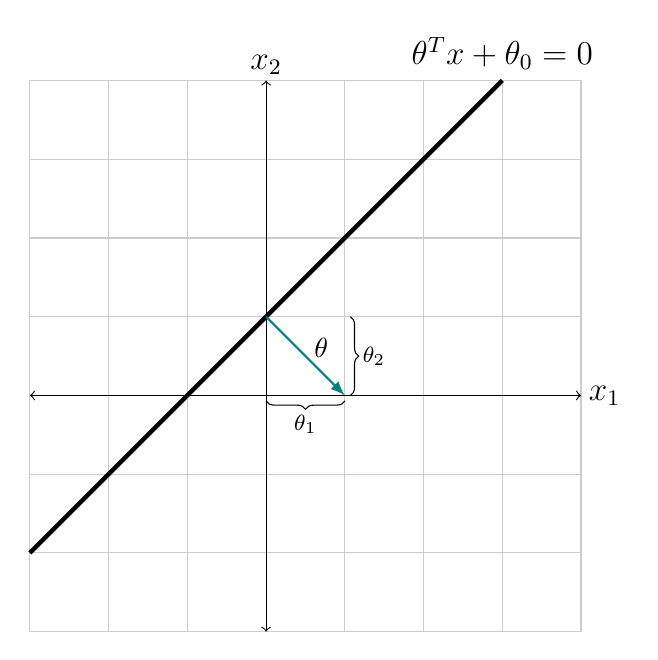
\begin{tikzpicture}
      \draw [thin, gray!40] (-3,-3) grid (4,4);
      \draw [<->] (-3,0) -- (4,0);
      \draw [<->] (0,-3) -- (0,4);

      \draw [ultra thick] (-3, -2) -- (3, 4)
      node [above] {\large$\theta^Tx + \theta_0 = 0$};

      \node [xshift=0em] at (4.3,0) {\large$x_1$};
      \node [xshift=0em] at (0,4.2) {\large$x_2$};

      % \draw [thick,teal,-latex] (0, 1) -- (0.9, 0.1)
      \draw [thick,teal,-latex] (0, 1) -- (1.0, 0.0)
      % node [black,below right] {$\theta$};
      node [black,midway, xshift=0.2cm,yshift=0.1cm] {$\theta$};

      \draw [decorate,decoration={brace,amplitude=3pt, mirror},xshift=2pt,yshift=0pt]
      (1,0) -- (1.0,1.0) node [black,midway,xshift=0.3cm]
      {\footnotesize $\theta_2$};

      \draw [decorate,decoration={brace,amplitude=3pt, mirror},xshift=0pt,yshift=-2pt]
      (0,0) -- (1.0,0.0) node [black,midway,yshift=-0.3cm]
      {\footnotesize $\theta_1$};
    \end{tikzpicture}

  \end{center}

  What is $\theta_0$?  We can solve for it by plugging a point
  on the line into the equation for the line.  It is often convenient to choose a point on one of the axes, e.g., in this case,
  $x=[0, 1]^T$, for which $\theta^T \left[ \begin{array}{c} 0 \\ 1 \end{array} \right] + \theta_0 = 0$, giving $\theta_0 = 1$.

\end{examplebox}

%%%%%%%%%%%%%%%%%%%%

In this example, the separator divides $\R^d$, the space our $\ex{x}{i}$ points live
in, into two half-spaces.  The one that is on the same side as the
normal vector is the {\em positive} half-space, and we classify all
points in that space as positive.  The half-space on the other side is
  {\em negative} and all points in it are classified as negative.

Note that we will call a separator a {\em linear separator}\index{separator!linear separator} of a data set
if all of the data with one label falls on one side of the separator and all of the
data with the other label falls on the other side of the separator. For instance, the
separator in the next example is a linear separator for the illustrated data. If there exists a linear separator on a dataset, we call this dataset {\em linearly separable}\index{linearly separable}.


\begin{examplebox}{\bf Example:}
  Let $h$ be the linear classifier defined by
  $\theta = \protect\twodcol{-1}{1.5}, \theta_0 = 3$.

  \noindent The diagram below shows several points classified by $h$.
  In particular, let $\ex{x}{1} = \twodcol{3}{2}$ and
  $\ex{x}{2} = \twodcol{4}{-1}$.
  \begin{align*}
    h(\ex{x}{1}; \theta, \theta_0) & = \sign\left(\twodrow{-1}{1.5}\twodcol{3}{2} + 3\right) = \sign(3) = +1     \\
    h(\ex{x}{2}; \theta, \theta_0) & = \sign\left(\twodrow{-1}{1.5}\twodcol{4}{-1} + 3\right) = \sign(-2.5) = -1
  \end{align*}
  Thus, $\ex{x}{1}$ and $\ex{x}{2}$ are given positive and negative classifications,
  respectively.

  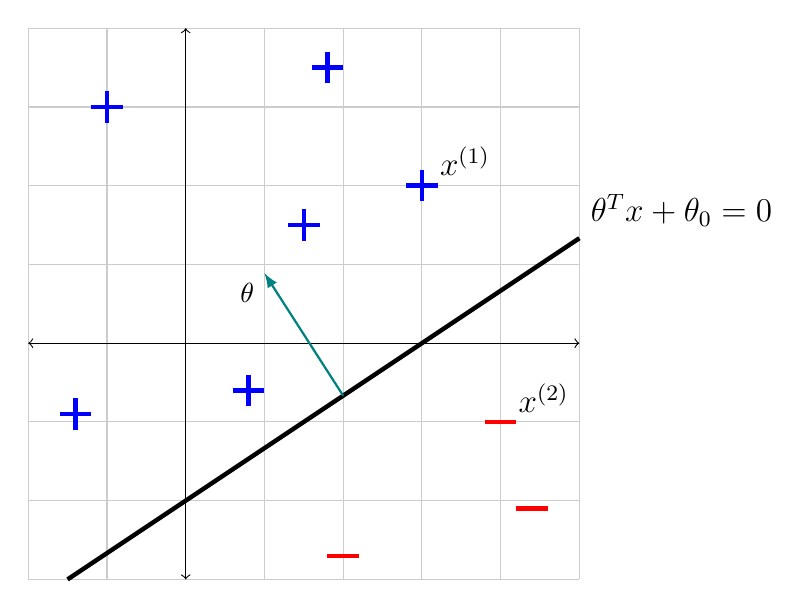
\begin{tikzpicture}
    \draw [thin, gray!40] (-2,-3) grid (5,4);
    \draw [<->] (-2,0) -- (5,0);
    \draw [<->] (0,-3) -- (0,4);

    \draw [ultra thick] (-1.5,-3) -- (5,1.3333)
    node [above right] {\large$\theta^Tx + \theta_0 = 0$};

    \draw [thick,teal,-latex] (2,-0.6667) -- (1,0.8883)
    node [black,below left] {$\theta$};

    \node [above right,xshift=.3em] at (3,2) {\large$\ex{x}{1}$};
    \node [above right,xshift=.3em] at (4,-1) {\large$\ex{x}{2}$};


    \foreach \Point in {(3,2), (1.8,3.5), (-1,3), (.8,-.6), (-1.4,-.9),
        (1.5, 1.5)}{
        \pic at \Point {plus};
      }

    \foreach \Point in {(4,-1), (2,-2.7), (4.4,-2.1)}{
        \pic at \Point {minus};
      }
  \end{tikzpicture}

\end{examplebox}

\question{What is the green vector normal to the separator?  Specify it
  as a column vector.}
\question{
  What change would you have to make to $\theta, \theta_0$ if you wanted
  to have the separating hyperplane in the same place, but to classify
  all the points labeled '+' in the diagram as negative and all the
  points labeled '-' in the diagram as positive?}


%%%%%%%%%%%%%%%%%%%%%%%%%%%%%%%%%%%%%%%%
%\subsection{Learning linear classifiers}

%% Now, given a data set and the hypothesis class of linear classifiers,
%% our goal will be to find the linear classifier that optimizes an
%% objective function relating its predictions to the training data.

%% {\em This is a well-formed optimization problem. But it's not
%%   computationally easy!} 

% We'll start by considering a very simple learning algorithm. \note{It's
%   a good idea to think of the ``stupidest possible'' solution to a
%   problem, before trying to get clever.  Here's a fairly (but not
%   completely) stupid algorithm.}  The idea is to generate $k$ possible
% hypotheses by generating their parameter vectors at random.  Then, we
% can evaluate the training-set error on each of the hypotheses and
% return the hypothesis that has the lowest training error (breaking
% ties arbitrarily). 

% \begin{codebox}
%   \Procname{$\proc{Random-Linear-Classifier}(\dataTrain, k)$}
%   \li \For $j \gets 1$ \To $k$
%   \li   \Do
%           randomly sample $\left(\ex{\theta}{j},
%             \ex{\theta_0}{j}\right)$ from $(\R^d, \R)$
%         \End
%   \li $j^* \gets \argmin{j \in \{1, \ldots, k\}} \mathcal{E}_n \left(\ex{\theta}{j}, \ex{\theta_0}{j}\right)$
%   \li \Return $\left(\ex{\theta}{j^*}, \ex{\theta_0}{j^*}\right)$
% \end{codebox}



% A note about terminology and 
% \anchorednote{notation.}
%  {The notation within the algorithm above might be new to you:
%   $\argmin{x} f(x)$ 
%   means the value of $x$ for which $f(x)$ is the smallest.  Sometimes
%   we write $\argmin{x \in {\cal X}} f(x)$ when we want to explicitly
%   specify the set ${\cal X}$ of values of $x$ over which we want to
%   minimize.}
% The training data $\dataTrain$ is an input to the learning algorithm,
% and the output of this learning algorithm will be a hypothesis $h$, where
% $h$ has parameters $\theta$ and $\theta_{0}.$ 
% In contrast to $\theta$ and $\theta_{0}$, the input $k$ is a 
% parameter of the learning algorithm itself; such
% parameters are often called {\em hyperparameters}.

% \question{
% What do you think will be observed for $\trainerr(h)$, where $h$ is the
% hypothesis returned by \proc{Random-Linear-Classifier}, if this learning
% algorithm is run multiple times? And as $k$ is increased? }

% \question{
%  What properties of $\dataTrain$ do you think will have an
% effect on $\trainerr(h)$?
% }

%%%%%%%%%%%%%%%%%%%%%%%%%%%%%%%%%%%%%%%%%%%%%%%%%%%%%%%%%%%%%%%%%%%%%%%%%%%%%
% Evaluating a learning algorithm -- moved to regression chapter 2021-08-04
%%%%%%%%%%%%%%%%%%%%%%%%%%%%%%%%%%%%%%%%%%%%%%%%%%%%%%%%%%%%%%%%%%%%%%%%%%%%%
% \section{Evaluating a learning algorithm}
% How should we evaluate the performance of a {\em classifier} $h$?   The best
% method is to measure {\em test error} on data that was not used to
% train it. 
% 
% How should we evaluate the performance of a {\em learning algorithm}?
% This is trickier.  There are many potential sources of variability in
% the possible result of computing test error on a learned hypothesis $h$:
% \begin{itemize}
% \item Which particular {\em training examples} occurred in $\dataTrain$
% \item Which particular {\em testing examples} occurred in $\dataTest$
% \item Randomization inside the learning {\em algorithm} itself
% \end{itemize}
% Generally, we would like to execute the following process multiple
% times: 
% \begin{itemize}
% \item Train on a new training set
% \item Evaluate resulting $h$ on a testing set {\em that does not
%     overlap the training set}
% \end{itemize}
% Doing this multiple times controls for possible poor choices of
% training set or unfortunate randomization inside the algorithm itself.
% 
% One concern is that we might need a lot of data to do this, and in
% many applications data is expensive or difficult to acquire. We can 
% re-use data with {\em{cross validation}} (but it's harder to do theoretical
% analysis).  \\
% \begin{codebox}
%   \Procname{$\proc{Cross-Validate}(\data, k)$}
%   \li divide $\data$ into $k$ chunks $\data_1, \data_2, \ldots \data_k$ (of roughly equal size)
%   \li \For $i \gets 1$ \To $k$
%   \li   \Do
%           train $h_i$ on $\data \setminus \data_i$ (withholding chunk $\data_i$)
%   \li     compute ``test'' error $\mathcal{E}_i (h_i)$ on withheld data $\data_i$
%         \End
%   \li \Return $\frac{1}{k} \sum_{i=1}^k \mathcal{E}_i (h_i)$
% \end{codebox}
% 
% It's very important to understand that cross-validation neither
% delivers nor evaluates a single particular hypothesis $h$.  It
% evaluates the {\em algorithm} that produces hypotheses.

%%%%%%%%%%%%%%%%%%%%%%%%%%%%%%%%%%%%%%%%%%%%%%%%%%%%%%%%%%%%%%%%%%%%%%%%%%%%%

% LPK: Try to keep \mathcal{L}(g, a) as much as possible
% LPK: Use cap Theta for all params

%%%%%%%%%%%%%%%%%%%%%%%%%%%%%%%%%%%%%%%%%%%%%%%%%%%%%%%%%%%%%%%%%%%%%%%%%%%%%
\section{Linear logistic classifiers}

\label{sec-lin_log_classifiers}

Given a data set and the hypothesis class of linear classifiers,
our goal will be to find the linear classifier that optimizes an
objective function relating its predictions to the training data.
To make this problem computationally reasonable, we will need to
take care in how we formulate the optimization problem to achieve
this goal.

For classification, it is natural to make predictions in $\{+1, -1\}$
and use the 0-1 loss function, $\mathcal{L}_{01}$, as introduced in Chapter~\ref{chap-intro}:
\[\mathcal{L}_{01}(g, a) = \begin{cases}
    0 & \text{if $g = a$} \\
    1 & \text{otherwise}
  \end{cases} \; .
\]
However, even for simple linear
classifiers, it is very difficult to
find values for $\theta, \theta_0$ that minimize simple 0-1 training error
\[J(\theta, \theta_0) = \frac{1}{n} \sum_{i=1}^n \mathcal{L}_{01}(\text{sign}(\theta^T\ex{x}{i} + \theta_0),
  \ex{y}{i})\;\;.\]
This problem is NP-hard, which probably
\note{The ``probably'' here is not because we're too lazy to look it
  up, but actually because of a fundamental unsolved problem in
  computer-science theory, known as ``P vs. NP.''}
implies
that solving the most difficult instances of this problem would
require computation time {\em exponential} in the number of training
examples, $n$.

What makes this a difficult optimization problem is its lack of
``smoothness'':
\begin{itemize}
  \item There can be two hypotheses, $(\theta, \theta_0)$  and
        $(\theta', \theta_0')$, where
        one is closer in parameter space to the optimal parameter values
        $(\theta^*, \theta_0^*)$, but they make the same number of
        misclassifications so they have the same $J$ value.
  \item All predictions are categorical:  the classifier can't express a
        degree of certainty about whether a particular input $x$ should have
        an associated value $y$.
\end{itemize}
For these reasons, if we are considering a hypothesis $\theta,\theta_0$
that makes five incorrect predictions, it is difficult to see how we
might change $\theta,\theta_0$ so that it will perform better, which
makes it difficult to design an algorithm that searches in a sensible
way through the
space of hypotheses for a good one.
For these reasons, we investigate another hypothesis class: {\em
linear logistic classifiers}, providing their definition, then an
approach for learning such classifiers using optimization.

%%%%%%%%%%%%%%%%%%%%%%%%%%%%%%%%%%%%%%%%
\subsection{Linear logistic classifiers: definition}

The hypotheses in a linear logistic classifier (LLC) are
parameterized by a $d$-dimensional vector $\theta$ and a scalar
$\theta_0$, just as is the case for linear classifiers.  However,
instead of making predictions in $\{+1, -1\}$, LLC hypotheses
generate real-valued outputs in the interval $(0, 1)$. An LLC has the form
\[h(x; \theta, \theta_0) = \sigma(\theta^T x + \theta_0)\;\;.\]
\index{linear logistic classifier}This looks familiar!  What's new?

The {\em logistic} function, also known as the {\em sigmoid} function,
is defined as
\[\sigma(z) = \frac{1}{1+e^{-z}}\;\;,\] and is plotted below, as a
function of its input $z$.
Its output can be interpreted as a probability, because for any value of
$z$ the output is in $(0, 1)$.

\begin{center}
  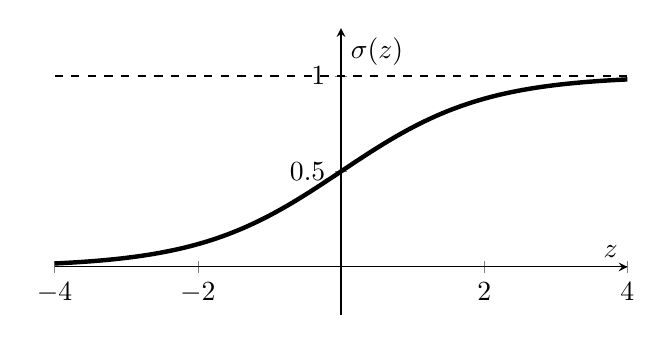
\begin{tikzpicture}
    \begin{axis}[
        axis lines=middle,
        % axis equal image,
        scale only axis,
        width=0.6\textwidth,
        height=0.3\textwidth,
        xmin=-4, xmax=4,
        ymin=-0.25, ymax=1.25,
        xlabel={$z$}, ylabel={$\sigma(z)$},
      ]
      \addplot [domain=-4:4, samples=100, ultra thick] {1/(1+exp(-x))};
      \addplot [domain=-4:4, samples=2, dashed] {1};
      \addplot [domain=-4:4, samples=2, dashed] {0};
    \end{axis}
  \end{tikzpicture}
\end{center}

\question{Convince yourself the output of $\sigma$ is always in the
  interval $(0, 1)$.  Why can't it equal 0 or equal 1?  For what value
  of $z$ does $\sigma(z) = 0.5$?}

What does an LLC look like?   Let's consider the
simple case where $d = 1$, so our input points simply lie along the
$x$ axis.  Classifiers in this case have dimension $0$, meaning that
they are points.
The plot below shows LLCs for three different parameter
settings: $\sigma(10x + 1)$, $\sigma(-2x + 1)$, and $\sigma(2x - 3).$
\begin{center}
  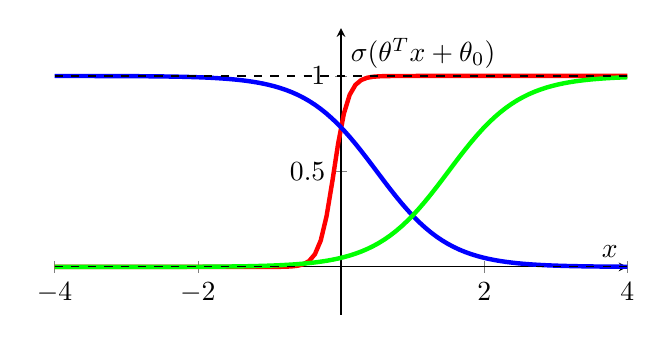
\begin{tikzpicture}
    \begin{axis}[
        axis lines=middle,
        % axis equal image,
        scale only axis,
        width=0.6\textwidth,
        height=0.3\textwidth,
        xmin=-4, xmax=4,
        ymin=-0.25, ymax=1.25,
        xlabel={$x$}, ylabel={$\sigma(\theta^T x + \theta_0)$},
      ]
      \addplot [domain=-4:4, samples=100, ultra thick, red] {1/(1+exp(-(10*x + 1)))};
      \addplot [domain=-4:4, samples=100, ultra thick, blue] {1/(1+exp(-(-2*x
        + 1)))};
      \addplot [domain=-4:4, samples=100, ultra thick, green] {1/(1+exp(-(2*x
        - 3)))};
      \addplot [domain=-4:4, samples=2, dashed] {1};
      \addplot [domain=-4:4, samples=2, dashed] {0};
    \end{axis}
  \end{tikzpicture}
\end{center}
\question{Which plot is which?  What governs the steepness of the
  curve?  What governs the $x$ value where the output is equal to
  0.5?}

But wait!  Remember that the definition of a classifier is that it's a mapping from $\R^d
  \rightarrow \{-1, +1\}$ or to some other discrete set.  So, then, it
seems like an LLC is actually not a classifier!

Given an LLC, with an output value in $(0, 1)$, what should we do if
we are forced to make a prediction in $\{+1, -1\}$?  A default answer
is to predict $+1$ if $\sigma(\theta^T x + \theta_0) > 0.5$ and $-1$
otherwise.  The value $0.5$ is sometimes called a {\em prediction
    threshold}.\index{logistic linear classifier!prediction threshold}

In fact, for different problem settings, we might prefer to pick a
different prediction threshold.  The field of {\em decision theory}
considers how to make this choice.
For example, if the consequences of predicting $+1$ when
the answer should be $-1$ are much worse than the consequences of
predicting $-1$ when the answer should be $+1$, then we might set the
prediction threshold to be greater than $0.5$.

\question{Using a prediction threshold of 0.5, for what values of $x$
  do each of the LLCs shown in the figure above predict $+1$?}

When $d = 2$, then our inputs $x$ lie in a two-dimensional space with
axes $x_1$ and $x_2$, and the output of the LLC is a surface, as shown
below, for $\theta = (1, 1), \theta_0 = 2$.

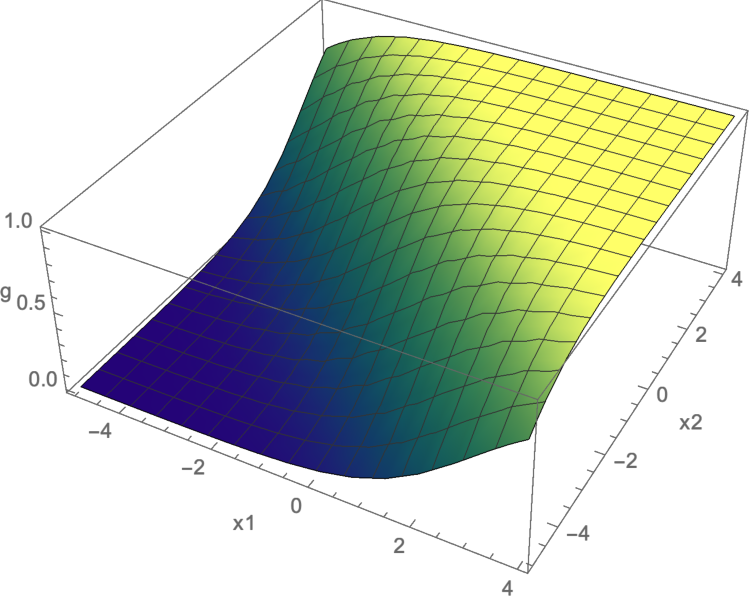
\includegraphics[width=0.7\textwidth]{figures/logreg3d}

\question{Convince yourself that the set of points for which
  $\sigma(\theta^T x + \theta_0) = 0.5$, that is, the ``boundary''
  between positive and negative predictions with prediction threshold
  $0.5$, is a line in $(x_1, x_2)$ space. What particular line is it
  for the case in the figure above?
  How would the plot change for $\theta = (1, 1)$, but now
  with $\theta_0 = -2$? For $\theta = (-1, -1), \theta_0 = 2$?}

%%%%%%%%%%%%%%%%%%%%%%%%%%%%%%%%%%%%%%%%
\subsection{Learning linear logistic classifiers}

\label{logistic}

Optimization is a key approach to solving machine learning
problems; this also applies to learning linear logistic classifiers (LLCs) by
defining an appropriate loss function for optimization.
A first attempt might be to use the simple 0-1 loss function $\mathcal{L}_{01}$
that gives a value of 0 for a correct prediction, and a 1 for an
incorrect prediction. As noted earlier, however, this gives rise
to an objective function that is very difficult to optimize, and so
we pursue another strategy for defining our objective.

For learning LLCs, we'd have a class of hypotheses
whose outputs are in $(0, 1)$, but for which we have training data with $y$
values in $\{+1, -1\}$.  How can we define an appropriate loss
function?  We start by changing our interpretation of the output to be
  {\em the probability that the input should map to output value 1} (we
might also say that this is the probability that the input is in class 1 or
that the input is `positive.')
\question{If $h(x)$ is the probability that $x$ belongs to class +1,
  what is the probability that $x$ belongs to the class -1? Assuming there are only these two classes.}

Intuitively, we would like to have
  {\em low loss if we assign a high probability to the correct class.}
We'll define a loss function, called {\em negative log-likelihood} (NLL)\index{negative log-likelihood},
that does just this.  In  addition, it has the cool property that it
extends nicely to the case where we would like to classify our inputs
into more than two classes.

In order to simplify the description, we assume that (or transform our
data so that) the labels
in the training data are $y \in \{0, 1\}$.
\note{\bf Remember to be sure your $y$
  values have this form if you try to learn an LLC using NLL!}

We would like to pick the parameters of our classifier to maximize the
probability assigned by the LLC to the correct $y$ values, as
specified in the training set.  Letting guess $\ex{g}{i} =
  \sigma(\theta^T\ex{x}{i} + \theta_0)$,
that probability is\note{That crazy huge $\Pi$ represents taking the
  product over a bunch of factors just as huge $\Sigma$ represents
  taking the sum over a bunch of terms.}
\begin{equation*}
  \prod_{i = 1}^n \begin{cases} \ex{g}{i} & \text{if $\ex{y}{i} =
              1$}                               \\ 1 - \ex{g}{i} & \text{otherwise}
  \end{cases}\;\;,
\end{equation*}
under the assumption that our predictions are independent.  This can
be cleverly rewritten, when $\ex{y}{i} \in \{0, 1\}$, as
\begin{equation*}
  \prod_{i = 1}^n {\ex{g}{i}}^{\ex{y}{i}}(1 - \ex{g}{i})^{1 - \ex{y}{i}}\;\;.
\end{equation*}
\question{Be sure you can see why these two expressions are  the
  same.}

The big product above is kind of hard to deal with in practice, though.
So what can we do?
Because the
log function is monotonic, the $\theta, \theta_0$ that maximize the
quantity above will be the same as the $\theta, \theta_0$ that
maximize its log, which is the following:
\begin{equation*}
  \sum_{i = 1}^n  \left( {\ex{y}{i}}\log {\ex{g}{i}} +
  (1 - \ex{y}{i})\log(1 - \ex{g}{i})\right)\;\;.
\end{equation*}
Finally, we can turn the maximization problem above into a minimization problem by taking the negative
of the above expression, and write in terms of minimizing a loss
\begin{equation*}
  \sum_{i = 1}^n \mathcal{L}_\text{nll}(\ex{g}{i}, \ex{y}{i})
\end{equation*}
where $\mathcal{L}_\text{nll}$ is the {\em negative log-likelihood}
loss function:
\begin{equation*}
  \mathcal{L}_\text{nll}(\text{guess},\text{actual}) =
  -\left(\text{actual}\cdot \log (\text{guess}) + (1 - \text{actual})\cdot\log (1 -
  \text{guess})\right) \;\;.
\end{equation*}
This loss function is also sometimes referred to as the {\em log loss}
or {\em cross entropy}\index{negative log-likelihood!loss function}. \note{You can use any base for the logarithm
  and it won't make any real difference.  If we ask you for numbers,
  use log base $e$.}

{\bf What is the objective function for linear logistic classification?}
We can finally put all these pieces together and develop an objective
function for optimizing regularized negative log-likelihood for a
linear logistic classifier. \note{That's a lot of fancy words!}  In
fact, this process is usually called ``logistic regression,'' so
we'll call our objective $J_\text{lr}$, and define it as
\begin{equation}
  J_\text{lr}(\theta, \theta_0; {\cal D}) =
  \left(\frac{1}{n} \sum_{i=1}^n
  \mathcal{L}_\text{nll}(\sigma(\theta^T \ex{x}{i} + \theta_0), \ex{y}{i})\right) +
  \lambda \norm{\theta}^2\;\;.
  \label{eq:lr_with_reg}
\end{equation}

\question{Consider the case of linearly separable data.   What will
  the $\theta$ values that optimize this objective be like if
  $\lambda = 0$?   What will they be like if $\lambda$ is very big?
  Try to work out an example in one dimension with two data points.}

{\bf What role does regularization play for classifiers?}
This objective function has the same structure as the one we used for
regression, Eq.~\ref{eq:ml_objective_loss}, where the first term (in
parentheses) is the average loss, and the second term is for regularization.
Regularization is needed for building classifiers that can generalize
well (just as was the case for regression).  The parameter $\lambda$ governs
the trade-off between the two terms as illustrated in the following example.


Suppose we wish to obtain a linear logistic classifier for this one-dimensional dataset:

\centerline{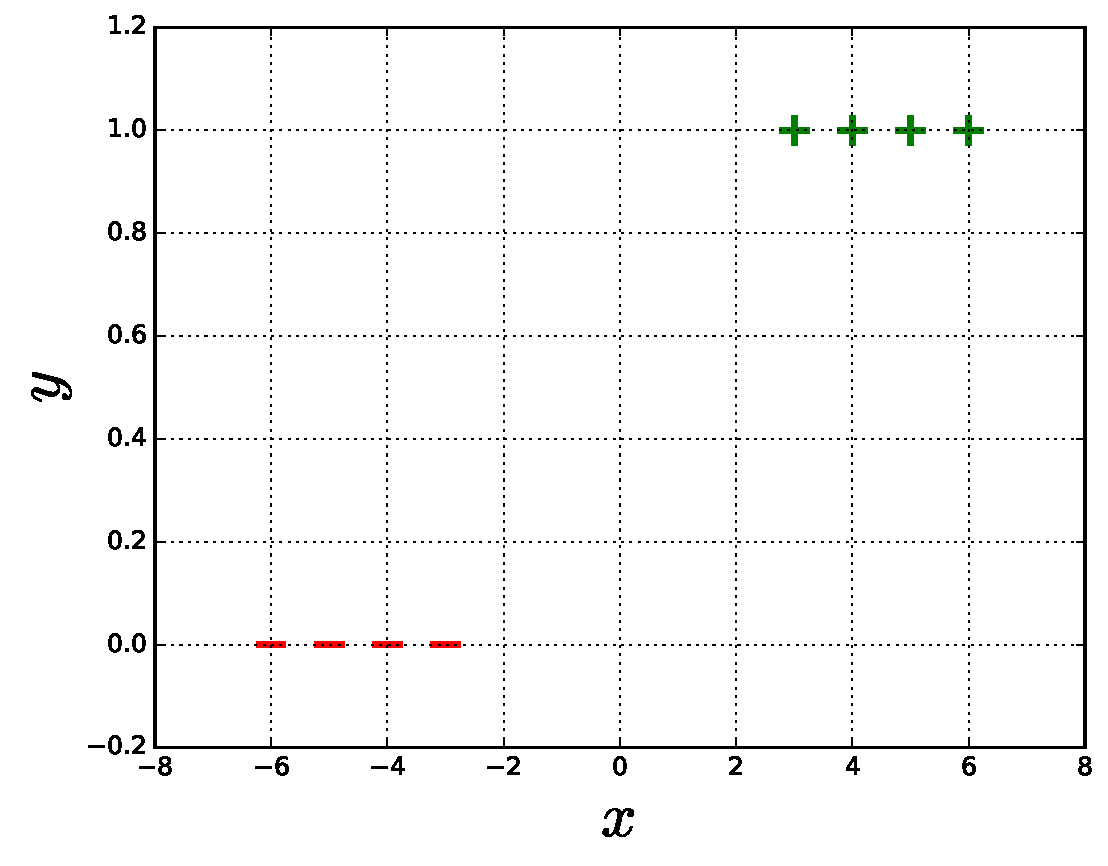
\includegraphics[width=0.45\textwidth]{figures/linear_logistic_classifier_and_regularization_data}}

%
\noindent
Clearly, this can be fit very nicely by a hypothesis
$h(x)=\sigma(\theta x)$, but what is the best value for $\theta$?
Evidently, when there is no regularization ($\lambda=0$), the objective function $J_{lr}(\theta)$ will approach zero for large
values of $\theta$, as shown in the plot on the left, below.
However, would the best hypothesis really have an infinite (or very
large) value for $\theta$?  Such a hypothesis would suggest that the
data indicate strong certainty that a sharp transition between $y=0$
and $y=1$ occurs exactly at $x=0$, despite the actual data having a wide
gap around $x=0$.
%
\centerline{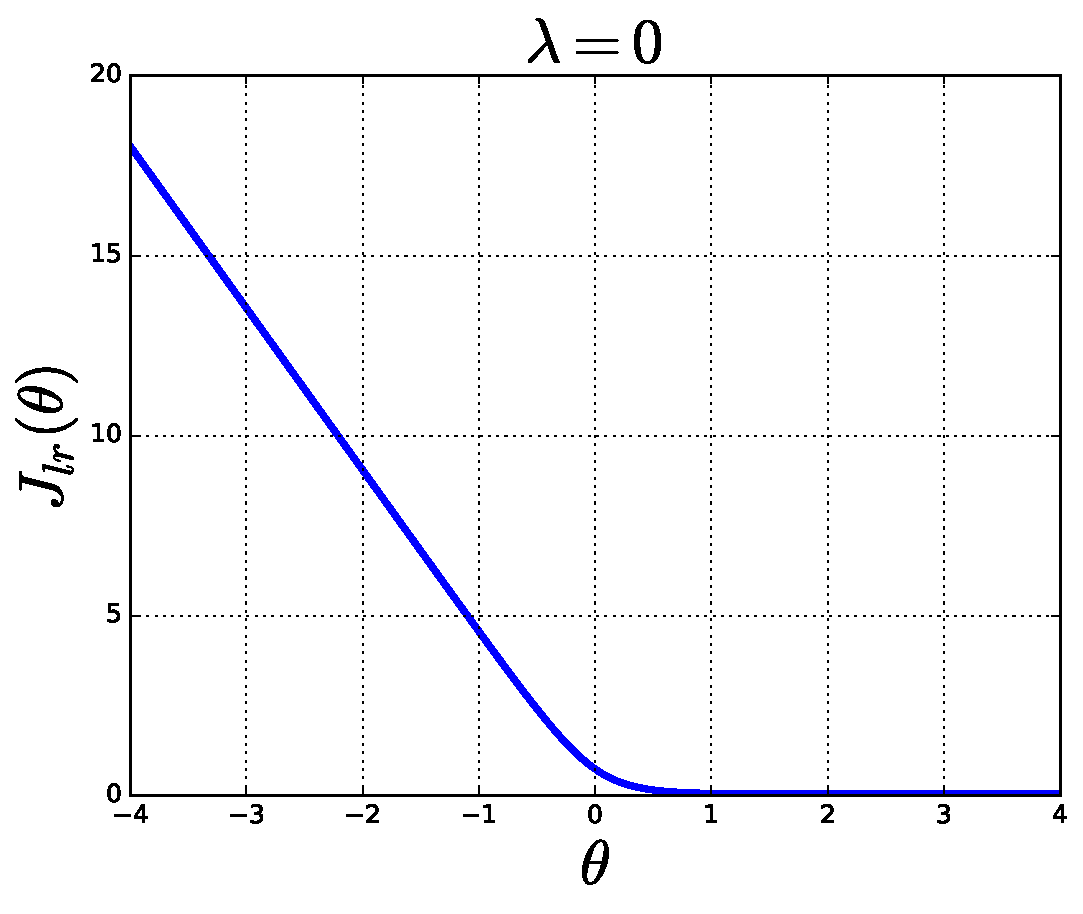
\includegraphics[width=0.45\textwidth]{figures/linear_logistic_classifier_and_regularization_objective_noreg}
  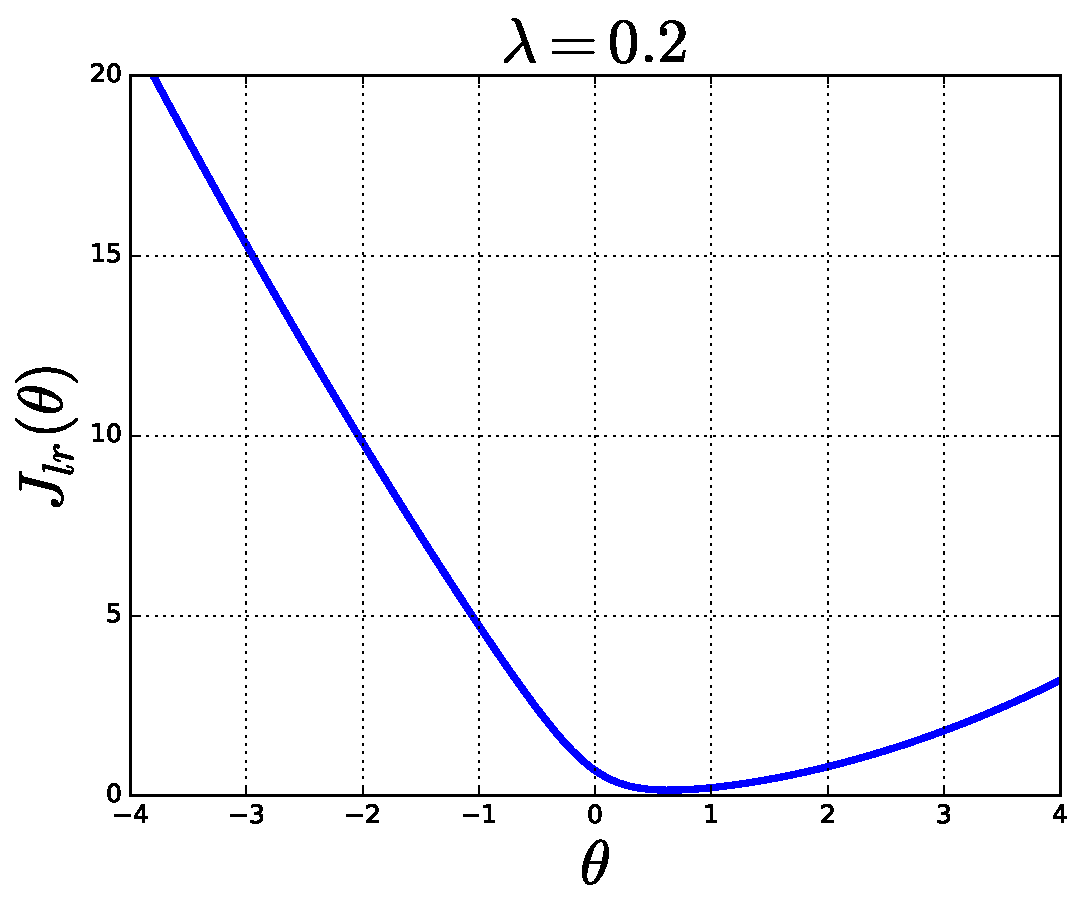
\includegraphics[width=0.45\textwidth]{figures/linear_logistic_classifier_and_regularization_objective_withreg}
}
%

\question{Be sure this makes sense.  When the $\theta$ values are
  very large, what does the sigmoid curve look like?  Why do we say
  that it has a strong certainty in that case?
}

In absence of other beliefs about the solution, we might prefer that
our linear logistic classifier not be overly certain about its
predictions, and so we might prefer a smaller $\theta$ over a large
$\theta.$ By not being overconfident, we might expect a somewhat
smaller $\theta$ to perform better on future examples drawn from this
same distribution.\note{To refresh on some vocabulary, we say that in
  this example, a very large $\theta$ would be {\em overfit} to the
  training data.}  This preference can be realized using a nonzero
value of the regularization trade-off parameter, as illustrated in the
plot on the right, above, with $\lambda=0.2$.

Another nice way of thinking about regularization is that we
would like to prevent our hypothesis from being too dependent on the
particular training data that we were given: we would like for it to
be the case that if the training data were changed slightly, the
hypothesis would not change by much.


% Hypothesis $h_1$ has zero training loss, but is
% very complicated.  Hypothesis $h_2$ mis-classifies two points, but is
% very simple.  In absence of other beliefs about the solution, it is
% often better to prefer that the solution be ``simpler,'' and so we
% might prefer $h_2$ over $h_1$, expecting it to perform better on
% future examples drawn from this same distribution.  \note{To establish
%   some vocabulary, we say that $h_1$ is {\em overfit} to the training
%   data.}  
% 
% \begin{center}
% \begin{tikzpicture}
%   \draw [->] (-4,0) -- (4,0);
%   \draw [->] (0,-4) -- (0,4);
%   \draw[red,thick] (-2.5,-3) .. controls (-4,1) and (-3.8,1.2) .. (-2.4,-.5)
%     .. controls (-2,-1) .. (-1,-1) .. controls (-.5,-1) ..  (.5,-2)
%     .. controls (.65, -2.1) .. (.7,-1.8) .. controls (.7,-1.5)
%     ..  (.6,-1.2) .. controls (.2,-.4) .. (1.2, -.3)
%     .. controls (1.6,-.2) .. (1,4);
% 
%   \foreach \Point in {(-3.4, .3), (2.5, .2), (-1.5,-2), (-1,-3),(.7,-.7),
%     (3, -2), (2.5, -3.2), (-.7,-1.2), (0.1,-1.8), (1.5, -1.5)}{
%     \draw \Point circle[radius=2pt];
%   }
%   \foreach \Point in {(.5,-1.7),(-.2,.3),(-2.8,.2),(-2.4,-.3),(-1,2.7),
%     (-1.5, 2), (-1.6, .9), (-3.8,-1), (-3.5,1.2),(.5, 1.2)}{
%   \fill \Point circle[radius=2pt];
%   }
%   \draw[blue, thick] (-3.5,-1.8) -- (3.5,1.3);
%   \node[right,blue] at (3.5,1.3) {$h_2$};
%   \node[below,right,red] at (1,4) {$h_1$};
% 
% \end{tikzpicture}
% \end{center}



\section{Gradient descent for logistic regression}

\label{sec-gd_lrr}

% Recall  that choosing a loss function is the
% first step in formulating a machine-learning problem as an
% optimization problem, and for regression we studied the mean square
% loss, Eq.~\ref{eq:reg_mse}, which captures loss as
% $({\rm guess} - {\rm actual})^2$.  The derivative of this,
% Eq.~\ref{eq:reg_gd_deriv}, was used previously to obtain an
% analytical solution to the linear regression problem.  Gradient
% descent could also be applied to numerically compute a solution, using
% the update rule
% \begin{equation}
%   \ex{\Theta}{t} = \ex{\Theta}{t-1} - \eta \frac{2}{n} \sum_{i=1}^{n} \left( \left[ \ex{\Theta}{t-1}\right]^T x^{(i)} - y^{(i)} \right) x^{(i)}
% \,.
% \end{equation}
% {~\hfill ~\note{Beware double superscripts!  $\left[ \Theta \right]^T$ is the transpose of the vector $\Theta$}}

% But what happens when the models are nonlinear, and the loss function
% is more complicated than being merely mean squared error?  Analytical
% solutions rarely exist for more complex situations, but gradient
% descent can still be applied, especially when the derivatives of the
% loss function can be computed analytically.  We will see this by
% applying gradient descent to $J_\text{lr}$, the logistic regression
% objective. 


% For classification, we
% are interested in the {\em negative log-likelihood} loss function
% (written more compactly as):
% \begin{equation}
%   \mathcal{L}_\text{nll}(\ex{g}{i}, \ex{y}{i})  = - {\ex{y}{i}}\log {\ex{g}{i}} - (1 - \ex{y}{i})\log(1 - \ex{g}{i})
% \;\;
% \end{equation}
% where the correct values $\ex{y}{i}$ are now assumed to be either $0$
% or $1$, and $\ex{g}{i}$ are our guesses.  These guesses are computed
% using the model parameters $\Theta = (\theta, \theta_0)$ as
% \begin{equation}
%   \ex{g}{i} = \sigma(\theta^T \ex{x}{i} + \theta_0)
% \,,
% \end{equation}
% where $\sigma$ is some {\em nonlinear} function which maps $\R$ to
% real numbers in the range $0$ to $1$ (inclusive of the endpoints).
% In what follows, we use the function $\sigma(z) = \frac{1}{1+e^{-z}}$. (See the next chapter for
% more intuition about why.)
% Combining this with a ridge regularization term, we obtain this
% ``logistic regression'' objective function:
% \begin{equation}
%   J_\text{lr}(\theta,\theta_0) = \frac{1}{n}\sum_{i=1}^n
%                                  \mathcal{L}_\text{nll}
%                                  (\ex{g}{i}, \ex{y}{i}) + \frac{\lambda}{2}\norm{\theta}^2
%                                \end{equation}

Now that we have a hypothesis class (LLC) and a loss function (NLL),
we need to take some data and find parameters!
Sadly, there is no lovely analytical solution like the one we obtained
for regression, in Section~\ref{sec-ridge_regression}.  Good thing we
studied gradient descent!  We can perform gradient descent on the
$J_{lr}$ objective, as we'll see next.  We can also apply stochastic
gradient descent to this problem.

Luckily, $J_{lr}$ has enough nice properties that gradient descent and
stochastic gradient descent should generally ``work''. We'll soon see
some more challenging optimization problems though -- in the
context of neural networks, in Section~\ref{sec-make_nn_work}.

First we need derivatives with respect to both $\theta_0$ (the scalar
component) and $\theta$ (the vector component) of $\Theta$.
Explicitly, they are: \note{Some passing familiarity with matrix
  derivatives is helpful here.  A foolproof way of computing them is
  to compute partial derivative of $J$ with respect to each component
  $\theta_i$ of $\theta$.}
\begin{align*}
  \nabla_\theta J_\text{lr}(\theta, \theta_0)                      & =  \frac{1}{n}\sum_{i=1}^n
  \left(\ex{g}{i} -
  \ex{y}{i}\right) \ex{x}{i}
  + 2\lambda\theta                                                                              \\
  \frac{\partial J_\text{lr}(\theta, \theta_0)}{\partial \theta_0} & =
  \frac{1}{n}\sum_{i=1}^n
  \left(\ex{g}{i} -
  \ex{y}{i} \right) \;\;.
\end{align*}
Note that $\nabla_\theta J_\text{lr}$ will be of shape $d \times 1$ and
$\frac{\partial J_\text{lr}}{\partial \theta_0}$ will be a scalar since
we have separated $\theta_0$ from $\theta$ here.
\question{Convince yourself that the dimensions of all these
  quantities are correct, under the assumption that $\theta$ is $d
    \times 1$. How does $d$ relate to $m$ as discussed for $\Theta$ in the
  previous section?
}

\question{Compute $\nabla_\theta \norm{\theta}^2$ by finding the
  vector of partial derivatives $(\partial \norm{\theta}^2 / \partial
    \theta_1, \ldots, \partial \norm{\theta}^2 / \partial
    \theta_d)$. What is the shape of $\nabla_\theta \norm{\theta}^2$?
}

\question{Compute $\nabla_\theta \mathcal{L}_\text{nll}(
  \sigma(\theta^T x + \theta_0), y)$ by finding the
vector of partial derivatives $(\partial \mathcal{L}_\text{nll}(
  \sigma(\theta^T x + \theta_0), y)/ \partial \theta_1, \ldots,
  \partial \mathcal{L}_\text{nll}(
  \sigma(\theta^T x + \theta_0), y) / \partial
  \theta_d)$.
  }

  \question{Use these last two results to verify our derivation above.}

  Putting everything together, our gradient descent algorithm for logistic
  regression becomes:\index{gradient descent!applied to logistic regression}
  \begin{codebox}
    \Procname{$\proc{LR-Gradient-Descent}(\theta_{\it init}, \theta_{0
          {\it init}},\eta,\epsilon)$}
    \li $\theta^{(0)} \gets \theta_{\it init}$
    \li $\theta_0^{(0)} \gets \theta_{0 {\it init}}$
    \li $t \gets 0$
    \li \Repeat
    \li   $t \gets t+1$
    \li   $\theta^{(t)} = \theta^{(t-1)} - \eta\left(\frac{1}{n}\sum_{i=1}^n
      \left(\sigma\left({\ex{\theta}{t-1}}^T \ex{x}{i} + \ex{\theta_0}{t-1}\right) -
        \ex{y}{i}\right) \ex{x}{i}
      + 2\lambda\ex{\theta}{t-1}
      \right)$
    \li   $\theta_0^{(t)} = \theta_0^{(t-1)} - \eta\left(\frac{1}{n}\sum_{i=1}^n
      \left(\sigma\left({\ex{\theta}{t-1}}^T \ex{x}{i} + \ex{\theta_0}{t-1}\right) -
        \ex{y}{i} \right)
      \right)$
    \li \Until $\left| J_{\text{lr}}(\theta^{(t)},\theta_0^{(t)}) - J_{\text{lr}}(\theta^{(t-1)},
      \theta_0^{(t-1)}) \right| <\epsilon$
    \li \Return $\theta^{(t)},\theta_0^{(t)}$
  \end{codebox}


  Logistic regression, implemented using batch or stochastic gradient
  descent, is a useful and fundamental machine learning technique. We
  will also see later that it corresponds to a one-layer neural network
  with a sigmoidal activation function, and so is an important step
  toward understanding neural networks.

  \subsection{Convexity of the NLL Loss Function}

  Much like the squared-error loss function that we saw for linear regression,
  the NLL loss function for linear logistic regression is a convex function.
  This means that running gradient descent with a reasonable set of hyperparameters
  will converge arbitrarily close to the minimum of the objective function.

  We will use the following facts to demonstrate that the NLL loss function is a convex function:
  \begin{itemize}
    \item if the derivative of a function of a scalar argument is monotonically increasing, then it is a convex function,
    \item the sum of convex functions is also convex,
    \item a convex function of an affine function is a convex function.
  \end{itemize}
  Let $z=\theta^T x + \theta_0$; $z$ is an affine function of $\theta$ and $\theta_0$.
  It therefore suffices to show that the functions $f_1(z) = - \log (\sigma(z))$ and
$f_2 (z) = -\log (1 - \sigma(z))$ are convex with respect to $z$.

  First, we can see that since,
  \begin{align*}
    \frac{d}{dz} f_1(z) & = \frac{d}{dz} \left[ -\log (1/(1 + \exp (-z))) \right], \\
                        & = \frac{d}{dz} \left[ \log (1 + \exp (-z)) \right],      \\
                        & = - \exp (-z) / (1 + \exp (-z)),                         \\
                        & = -1 + \sigma(z),
  \end{align*}
  the derivative of the function $f_1 (z)$ is a monotonically increasing function and
  therefore $f_1$ is a convex function.

  Second, we can see that since,
  \begin{align*}
    \frac{d}{dz} f_2(z) & = \frac{d}{dz} \left[ -\log (\exp(-z)/(1 + \exp (-z))) \right], \\
                        & = \frac{d}{dz} \left[ \log (1 + \exp (-z)) + z \right],         \\
                        & = \sigma(z),
  \end{align*}
  the derivative of the function $f_2(z)$ is also monotonically increasing and
  therefore $f_2$ is a convex function.

  \section{Handling multiple classes}

  So far, we have focused on the {\em binary} classification case, with
  only two possible classes.  But what can we do if we have multiple
  possible classes (e.g., we want to predict the genre of a movie)?
  There are two basic strategies:
  \begin{itemize}
    \item Train multiple binary classifiers using different subsets of
          our data and combine their outputs to make a class prediction.
    \item Directly train a multi-class classifier using a hypothesis
          class that is a generalization of logistic regression, using a
            {\em one-hot} output encoding and NLL loss.
  \end{itemize}

  %% We will explore both methods below, but the method based on NLL is
  %% in wider use, especially in the context of neural networks.

  %% \subsection{Reducing multi-class to binary}

  %% There are two standard strategies for reducing multi-class
  %% classification to binary classification.\index{classification!multi-class classification}

  %% In the {\em one versus all} (OVA) strategy\index{classification!multi-class classification!one versus all}, we will train $K$
  %% different binary classifiers.  To train classifier $k$, we
  %% \begin{itemize}
  %% \item Create a training set $\data_k$ in which all $\ex{x}{i} \in D$
  %%   for which $\ex{y}{i} = k$ are assigned label $+1$ and all other
  %%   $\ex{x}{i}$ are assigned label $-1$.
  %% \item Use logistic regression (or any other classifier-learning
  %%   method) to obtain a hypothesis $h_k$ by training on $\data_k$.
  %%   \end{itemize}
  %% Then, we create a new multi-class hypothesis 
  %%   \[h(x) = \argmax{k} h_k(x)\;\;,\]
  %%   that predicts the class $k$ to which this example was
  %%   assigned with highest confidence by the individual hypotheses.

  %%   In the {\em one versus one} (OVO) strategy\index{classification!multi-class classification!one versus one}, we will train
  %% $K(K-1)/2$ classifiers, one for each unique pair $j, k$ (where $j \not= k$) of classes.  To
  %% train classifier $j, k$, we
  %% \begin{itemize}
  %% \item Create a training set $\data_{jk}$ in which all $\ex{x}{i} \in D$
  %%   for which $\ex{y}{i} = j$ are assigned label $+1$ and
  %%  all $\ex{x}{i} \in D$ for which $\ex{y}{i} = k$ are assigned label $-1$.
  %% \item Use logistic regression (or any other classifier-learning
  %%   method) to obtain hypotheses $h_{jk}$ by training on $\data_{jk}$.
  %% \end{itemize}
  %% Then, given a new input $x$, we feed it into each of the classifiers $h_{jk}$
  %% and obtain a {\em binary} decision about whether it is more likely to
  %% be in class $j$ or class $k$.  We generate as output the class that is
  %% selected as the ``winner'' in the majority of the cases.

  %% \subsection{Multi-class classification and log likelihood}

  The method based on NLL is in wider use, especially in the context of
  neural networks, and is explored here.
  In the following, we will assume that we have a data set $\data$ in
  which the inputs
$\ex{x}{i} \in R^d$ but the outputs $\ex{y}{i}$ are drawn from a set
  of $K$ classes $\{c_1, \ldots, c_K\}$.
  Next, we extend the idea of NLL directly to multi-class
  classification\index{negative log-likelihood!multi-class
    classification} with $K$ classes, where the training label is
  represented with what is called a {\em one-hot} vector
$y=\begin{bmatrix} y_1, \ldots, y_K \end{bmatrix}^T$, where $y_k=1$ if
  the example is of class $k$ and $y_k = 0$ otherwise.
  Now, we have a problem of mapping an input $\ex{x}{i}$ that is in
$\R^d$ into a $K$-dimensional output.  Furthermore, we would like this
  output to be interpretable as a discrete probability distribution over
  the possible classes, which means the elements of the output vector have to
  be {\em non-negative} (greater than or equal to 0) and sum to 1.

  We will do this in two steps.  First, we will map our input
$\ex{x}{i}$ into a vector value $\ex{z}{i} \in \R^K$ by letting $\theta$ be a
  whole $d \times K$ {\em matrix} of parameters, and $\theta_0$ be a $K
\times 1$ vector, so that
  \[z = \theta^T x + \theta_0\;\;.\]
  \note{Let's check dimensions!  $\theta^T$ is $K \times d$ and $x$ is
    $d \times 1$, and $\theta_0$ is $K \times 1$, so $z$ is $K \times
      1$ and we're good!}
  Next, we have to extend our use of the sigmoid function to the
  multi-dimensional {\em softmax} function, that takes
  a whole vector $z \in \R^K$ and generates
  \[g = \textit{softmax}(z) =
    \begin{bmatrix}
      \exp(z_1) / \sum_{i} \exp(z_i) \\
      \vdots                         \\
      \exp(z_K) / \sum_{i} \exp(z_i)
    \end{bmatrix}\;\;.\]
  which can be interpreted as a probability distribution over $K$ items. To make the final prediction of the class label, we can then look at $g,$ find the most likely probability over these $K$ entries in $g,$ (i.e. find the largest entry in $g,$) and return the corresponding index as the ``one-hot'' element of $1$ in our prediction.

  \question{Convince yourself that the vector of $g$ values will be
    non-negative and sum to 1.}

  Putting these steps together, our hypotheses will be
  \[h(x; \theta, \theta_0) = \textit{softmax}(\theta^T x + \theta_0)\;\;.\]

  Now, we retain the goal of maximizing the probability that our
  hypothesis assigns to the correct output $y_k$ for each input $x$.  We
  can write this probability, letting $g$ stand for our ``guess'', $h(x)$, for a
  single example $(x, y)$ as $\prod_{k = 1}^K g_k^{y_k}$.
  \question{How many elements that are not equal to 1 will there be in this product?}

  The negative log of the probability that we are making a correct guess is, then, for {\em one-hot} vector $y$ and {\em probability distribution}
  vector $g$,
$$\mathcal{L}_\text{nllm}(\text{g},\text{y}) =
  - \sum_{k=1}^K \text{y}_k \cdot \log(\text{g}_k) \;\;.$$
We'll call this {\sc nllm} for {\em negative log likelihood
    multiclass.} It is also worth noting that the NLLM loss function is also convex; however, we will omit the proof.
\question{Be sure you see that is $\mathcal{L}_\text{nllm}$ is minimized when the guess assigns high probability to the true class.}
\question{Show that $\mathcal{L}_\text{nllm}$ for $K = 2$ is the same as
  $\mathcal{L}_\text{nll}$. }

\section{Prediction accuracy and validation}

In order to formulate classification with a smooth objective function
that we can optimize robustly using gradient descent, we changed the
output from discrete classes to probability values and the loss
function from 0-1 loss to NLL.
However, when time comes to actually make a prediction we usually have
to make a hard choice:  buy stock in Acme or not?  And, we get
rewarded if we guessed right, independent of how sure or not we were
when we made the guess.

The performance of a classifier is often characterized by its {\em
    accuracy}, which is the percentage of a data set that it predicts
correctly in the case of 0-1 loss. We can see that accuracy of hypothesis $h$ on data $\data$
is the fraction of the data set that does not incur any loss:
\[A(h; \data) = 1 - \frac{1}{n}\sum_{i=1}^n\mathcal{L}_{01}(\ex{g}{i}, \ex{y}{i})\;\;,\]
where $\ex{g}{i}$ is the final guess for one class or the other
that we make from $h(\ex{x}{i})$, e.g., after thresholding.
It's noteworthy here that we use a different loss function for optimization
than for evaluation. This is a compromise we make for computational
ease and efficiency.



%%% Local Variables:
%%% mode: latex
%%% TeX-master: "top"
%%% End:


\chapter{Feature representation}
\label{chap-features}

Linear regression and classification are powerful tools, but in the real world, data often
exhibit {\em non-linear} behavior that cannot immediately be
captured by the linear models which we have built so far.  For example,
suppose the true behavior of a system (with $d=2$) looks like this
wavelet: \note{This plot is of the so-called {\em jinc}
function $J_1(\rho)/\rho$ for $\rho^2=x_1^2 + x_2^2$}
%
% Note rho is radial distance squared, because we don't want to have to use
% a sqrt in the polynomial basis

\centerline{\includegraphics[width=0.5\textwidth]{figures/regression_features1_sombrero_comp1.pdf}}

\noindent
Such behavior is actually ubiquitous in physical systems, e.g., in the
vibrations of the surface of a drum, or scattering of light through an
aperture.  However, no single hyperplane would be a very good fit to
such peaked responses!

A richer class of hypotheses can be obtained by performing a
non-linear feature transformation $\phi(x)$ before doing the
regression. That is, $\theta^Tx + \theta_0$ is a linear function of
$x$, but $\theta^T\phi(x) + \theta_0$ is a non-linear function of $x,$
if $\phi$ is a non-linear function of $x$.

There are many different ways to construct $\phi$.  Some are
relatively systematic and domain independent.
Others are directly related to the semantics (meaning) of the original
features, and we construct them deliberately with our application (goal) in mind.

%%%%%%%%%%%%%%%%%%%%%%%%%%%%%%%%%%%%%%%%%%%%%%%%%%%%%%%%%%%%%%%%%%%%%%%%%%%%%
\section{Gaining intuition about feature transformations}

\label{sec-features_classifiers}

In this section, we explore the effects of non-linear feature
transformations on simple classification problems, to gain intuition.



% There is no linear separator for this two-dimensional dataset!  But, we have a trick
% available:  take a low-dimensional data set and move it, using a
% non-linear transformation into a higher-dimensional space, and look
% for a linear separator there.

Let's look at an example data set that starts in 1-D:

\begin{examplebox}
  \begin{center}
    \begin{tikzpicture}
      \draw [<->, gray] (-3,0) -- (3,0)
      node [black, right] {$x$};
      \draw [gray] (0,.6) -- (0,-.6)
      node [black, below] {0};

      \pic at (-1.5, 0) {plusblk};
      \pic at (-.5, 0) {minusblk};
      \pic at (.5, 0) {minusblk};
      \pic at (1.5, 0) {plusblk};

    \end{tikzpicture}
  \end{center}
\end{examplebox}

These points are not linearly separable, \note{What's a linear
  separator for data in 1D?  A point!}  but consider the
transformation $\phi(x) = [x,x^2]^T$. Putting the data in $\phi$ space,
we see that it is now separable.  There are lots of possible
separators;  we have just shown one of them here.

\begin{examplebox}
  \begin{center}
    \begin{tikzpicture}
      \draw [<->, gray] (-3,0) -- (3,0)
      node [black, right] {$x$};
      \draw [<->, gray] (0,-.6) -- (0,4)
      node [black, above] {$x^2$};

      \draw [dashed] (-3, 1.25) -- (3, 1.25)
      node [below, xshift=-1cm] {separator};

      \pic at (-1.5, 2.25) {plusblk};
      \pic at (-.5, .25) {minusblk};
      \pic at (.5, .25) {minusblk};
      \pic at (1.5, 2.25) {plusblk};

    \end{tikzpicture}
  \end{center}
\end{examplebox}

A linear separator in $\phi$ space is a nonlinear separator in the
original space!  Let's see how this plays out in our simple example.
Consider the separator $x^2  - 1 = 0$, which labels the half-plane
$x^2 -1 > 0$ as positive.  What separator does it correspond to in the
original 1-D space?
We have to ask the question:  which $x$ values have the property that
$x^2 - 1 = 0$.  The answer is $+1$ and $-1$, so those two points
constitute our separator, back in the original space.  And we can use
the same reasoning to find the region of 1D space that is labeled
positive by this separator.

\begin{examplebox}
  \begin{center}
    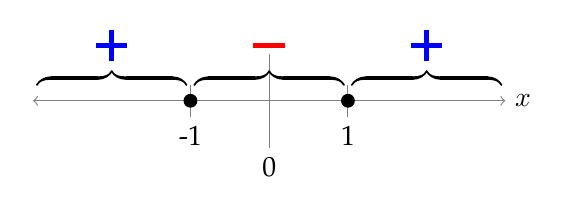
\begin{tikzpicture}
      \draw [<->, gray] (-3,0) -- (3,0)
      node [black, right] {$x$};
      \draw [gray] (0,.6) -- (0,-.6)
      node [black, below] {0};
      \draw [gray] (1,.2) -- (1,-.2)
      node [black, below] {1};
      \draw [gray] (-1,.2) -- (-1,-.2)
      node [black, below] {-1};

      \fill (1,0) circle (2.5pt);
      \fill (-1,0) circle (2.5pt);

      \draw[decoration={calligraphic brace,amplitude=5pt}, decorate, line width=1.25pt]
      (-2.95,0.2) node {} -- (-1.05,0.2);
      \draw[decoration={calligraphic brace,amplitude=5pt}, decorate, line width=1.25pt]
      (-.95,0.2) node {} -- (.95,0.2);
      \draw[decoration={calligraphic brace,amplitude=5pt}, decorate, line width=1.25pt]
      (1.05,0.2) node {} -- (2.95,0.2);

      \pic at (-2, 0.7) {plus};
      \pic at (0, 0.7) {minus};
      \pic at (2, 0.7) {plus};

    \end{tikzpicture}
  \end{center}
\end{examplebox}




%%%%%%%%%%%%%%%%%%%%%%%%%%%%%%%%%%%%%%%%%%%%%%%%%%%%%%%%%%%%%%%%%%%%%%%%%%%%%
\section{Systematic feature construction}
Here are two different ways to systematically construct features in a
  {\em problem independent} way.

\subsection{Polynomial basis}

\label{polyBasis}

If the features in your problem are already naturally numerical, one
systematic strategy for constructing a new feature space is to use a
  {\em polynomial basis}\index{basis functions!polynomial basis}.  The idea is that, if you are using the
$k$th-order basis (where $k$ is a positive integer), you include a
feature for every possible product of $k$ different dimensions in your
original input.

Here is a table illustrating the $k$th order polynomial basis for
different values of $k$, calling out the cases when $d=1$ and $d>1$:

\begin{center}
  \begin{tabular}{c c c}
    Order  & $d=1$             & in general ($d>1$)       \\
    \hline
    0      & $[1]$             & $[1]$                    \\
    1      & $[1,x]^T$         & $[1,x_1, \ldots, x_d]^T$ \\
    2      & $[1,x,x^2]^T$     & $[1,x_1, \ldots, x_d,
    x_1^2, x_1x_2, \ldots]^T$                             \\
    3      & $[1,x,x^2,x^3]^T$ & $[1,x_1, \ldots,
          x_1^2, x_1x_2, \ldots,
    x_1x_2x_3, \ldots]^T$                                 \\
    \vdots & \vdots            & \vdots
  \end{tabular}
\end{center}

This transformation can be used in combination with linear regression
or logistic regression (or any other regression or classification
model).  When we're using a linear regression or classification model,
the key insight is that a linear regressor or separator in the {\em
    transformed space} is a non-linear regressor or separator in the
original space.


% (* capture jinc function with features *)
% 
% npts = 1000;
% SeedRandom[1];
% x1 = RandomReal[{-rm, rm}, {npts}]; 
% x2 = RandomReal[{-rm, rm}, {npts}]; 
% r = (x1)^2 + (x2)^2;
% yv = BesselJ[1, r]/r;
% pts = Transpose@{x1, x2, yv};
% model = LinearModelFit[
%    pts, {  1, 
%     Subscript[x, 1]^2 + 
%      Subscript[x, 2]^2, (Subscript[x, 1]^2 + Subscript[x, 2]^2)^2,
%     (Subscript[x, 1]^2 + Subscript[x, 2]^2)^4}, { Subscript[x, 1], 
%     Subscript[x, 2]}];
% 
% vp = {1.207331108916506`, -3.0537082213398925`, 0.8168339441793491`};
% 
% p1 = ListPointPlot3D[ pts, 
%    AxesLabel -> {Subscript[x, 1], Subscript[x, 2], y}, 
%    PlotRange -> {0, 0.6}, ViewPoint -> vp ];
% p3 = Plot3D[
%    model[Subscript[x, 1], Subscript[x, 2]], {Subscript[x, 1], -rm, 
%     rm}, {Subscript[x, 2], -rm, rm}, PlotStyle -> Opacity[0.2], 
%    PlotRange -> {0, 0.6}, PlotPoints -> 100];
% p4 = Show[{p1, p3}];
% gr1 = GraphicsRow[{p1, p4}, ImageSize -> Large]
% Export["regression_features2_fitsombrero.png", gr1, 
%   ImageResolution -> 1200]; 

For example, the wavelet pictured at the start of this chapter can be
fit much better than with just a hyperplane, using linear regression
with polynomials\anchorednote{up to order $k=8$:}{Specifically, this
  example uses $[1, x_1, x_2, x_1^2 + x_2^2, (x_1^2 + x_2^2)^2, (x_1^2 + x_2^2)^4]^T$ }

\centerline{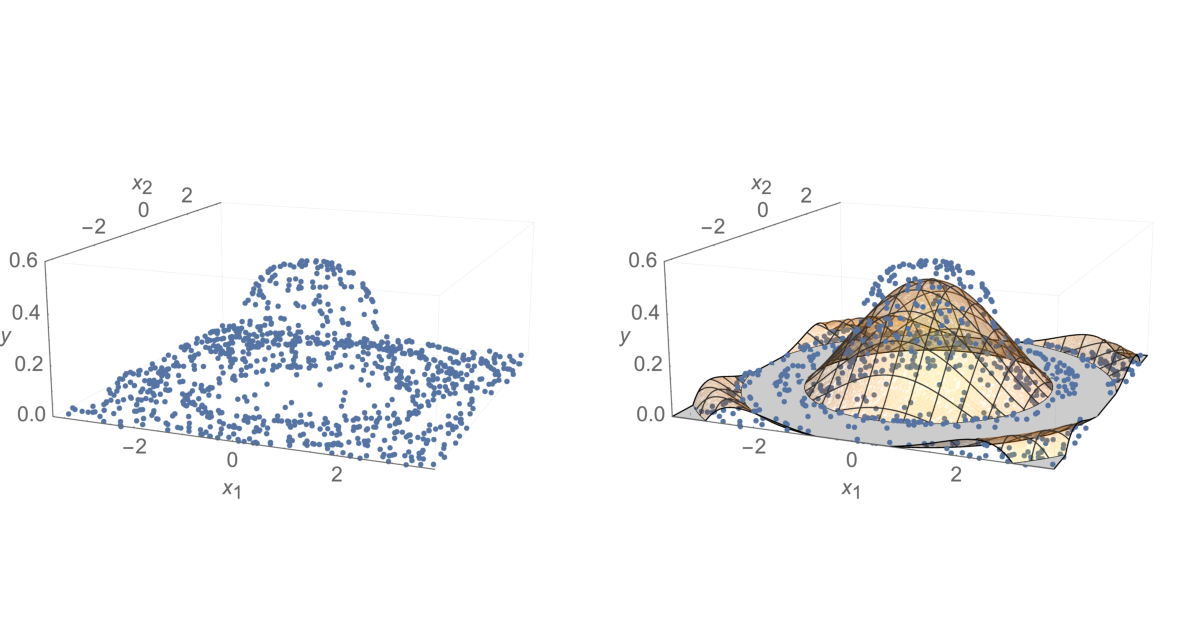
\includegraphics[width=0.9\textwidth]{figures/regression_features2_fitsombrero.pdf}}

\noindent
The raw data (with $n=1000$ random samples) is plotted on the left, and the regression result (curved surface) is on the right.

% \question{
% What polynomial terms would be needed for a good basis of features, if the wavelet were centered somewhere other than at the origin?
% }

Now let's look at a classification example and see how polynomial feature transformation may help us.

One well-known example is the ``exclusive or'' ({\sc xor}) data set, the drosophila \note{D. Melanogaster is a species of fruit fly, used as a simple system in which to study genetics, since 1910.} of machine-learning data sets:

\begin{examplebox}
  \begin{center}
    \begin{tikzpicture}
      \pic at (-1, -1) {plusblk};
      \pic at (-1, +1) {minusblk};
      \pic at (+1, -1) {minusblk};
      \pic at (+1, +1) {plusblk};
    \end{tikzpicture}
  \end{center}
\end{examplebox}

Clearly, this data set is not linearly separable. So, what if we try to solve the {\sc xor} classification problem using a polynomial
basis as the feature transformation?  We can just take our
two-dimensional data and transform it into a higher-dimensional data
set, by applying $\phi$.  Now, we have a classification problem as
usual.

Let's try it for $k = 2$ on our {\sc xor} problem.  The feature
transformation is
\[\phi([x_1, x_2]^T) = [1, x_1, x_2, x_1^2, x_1 x_2, x_2^2]^T\;\;.\]
\question{
  If we train a classifier after performing this feature
  transformation, would we lose any expressive
  power if we let $\theta_0 = 0$ (i.e., trained without offset instead of
  with offset)?}
We might run a classification learning algorithm and find a separator
with coefficients $\theta = [0, 0, 0, 0, 4, 0]^T$ and $\theta_0 = 0$.
This corresponds to
\[0 + 0 x_1 + 0 x_2 + 0 x_1^2 + 4 x_1 x_2 + 0x_2^2 + 0 = 0\]
and is plotted below, with the gray shaded region classified as
negative and the white region classified as positive:
\begin{examplebox}
  \begin{center}
    % 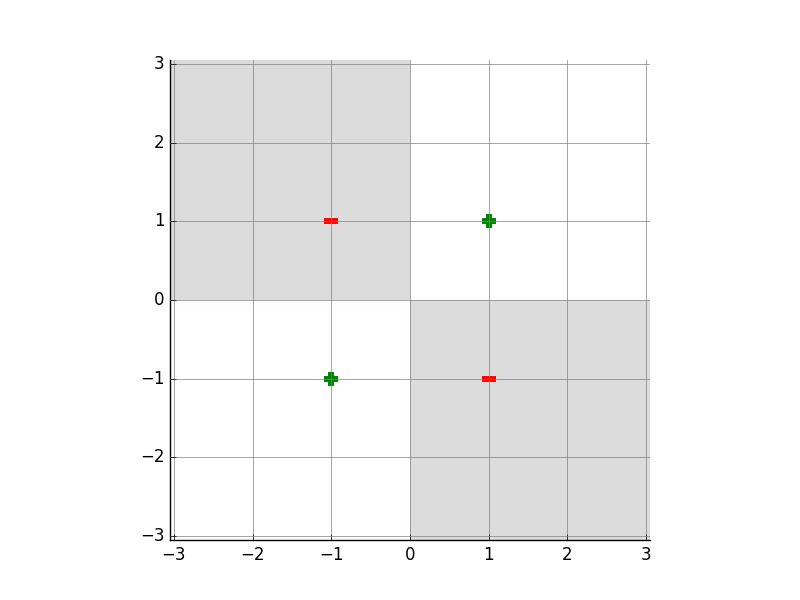
\includegraphics[scale=0.3]{figures/feature_representation_1.png}
    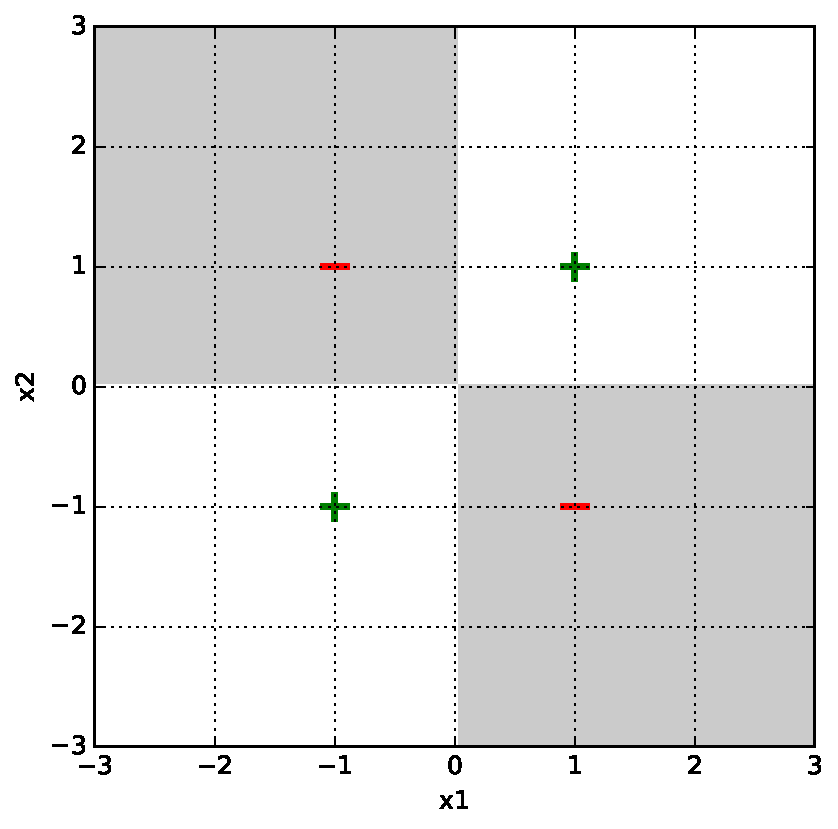
\includegraphics[scale=0.48]{figures/feature_representation_xor_sign.pdf}
  \end{center}
\end{examplebox}
\question{
  Be sure you understand why this high-dimensional hyperplane is a
  separator, and how it corresponds to the figure.}

For fun, we show some more plots below.  Here is another result for a
linear classifier on {\sc xor} generated with logistic regression and
gradient descent, using a random initial starting point and second-order
polynomial basis:

\begin{examplebox}
  \begin{center}
    % 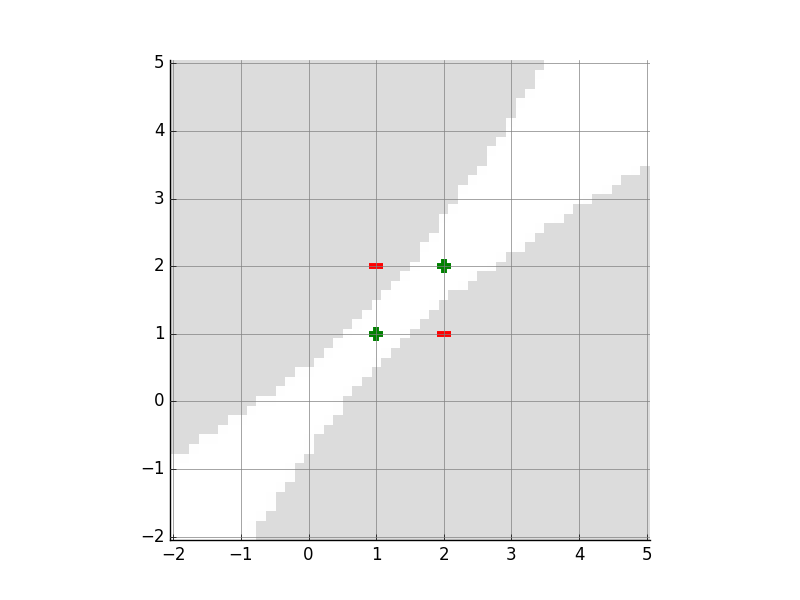
\includegraphics[scale=0.3]{figures/feature_representation_2.png}
    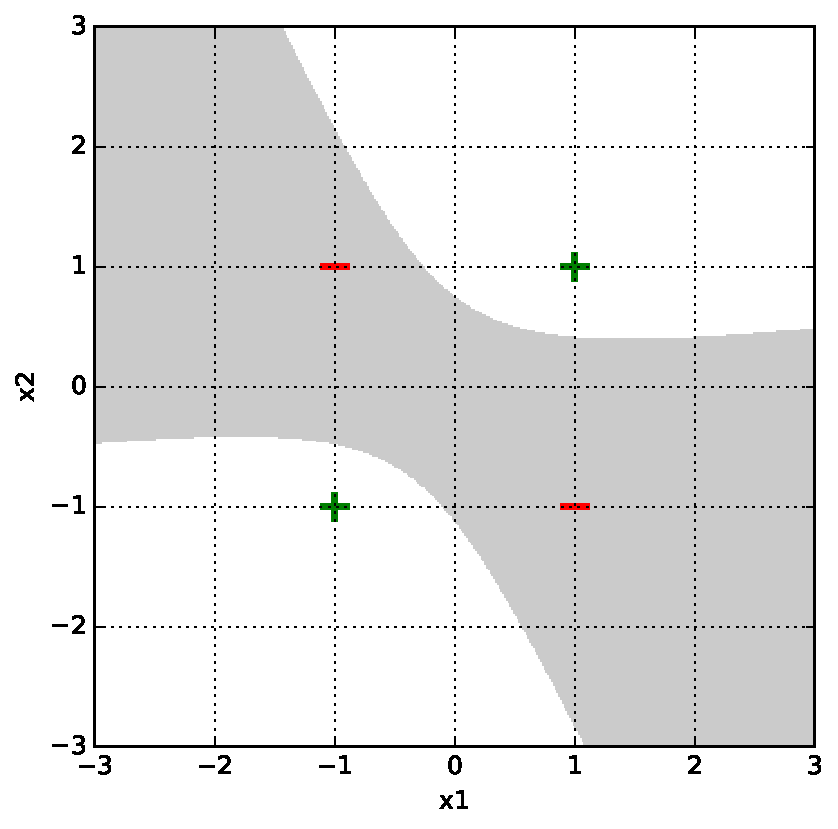
\includegraphics[scale=0.48]{figures/feature_representation_xor_order2.pdf}
  \end{center}
\end{examplebox}

Here is a harder data set.  Logistic regression with gradient descent
failed to separate it with a second, third, or fourth-order basis feature
representation, but succeeded with a fifth-order basis.
Shown below are some results after $\sim1000$
gradient descent iterations (from random starting points) for bases of
order 2 (upper left), 3 (upper right), 4 (lower left), and 5 (lower right).
\begin{examplebox}
  \begin{center}
    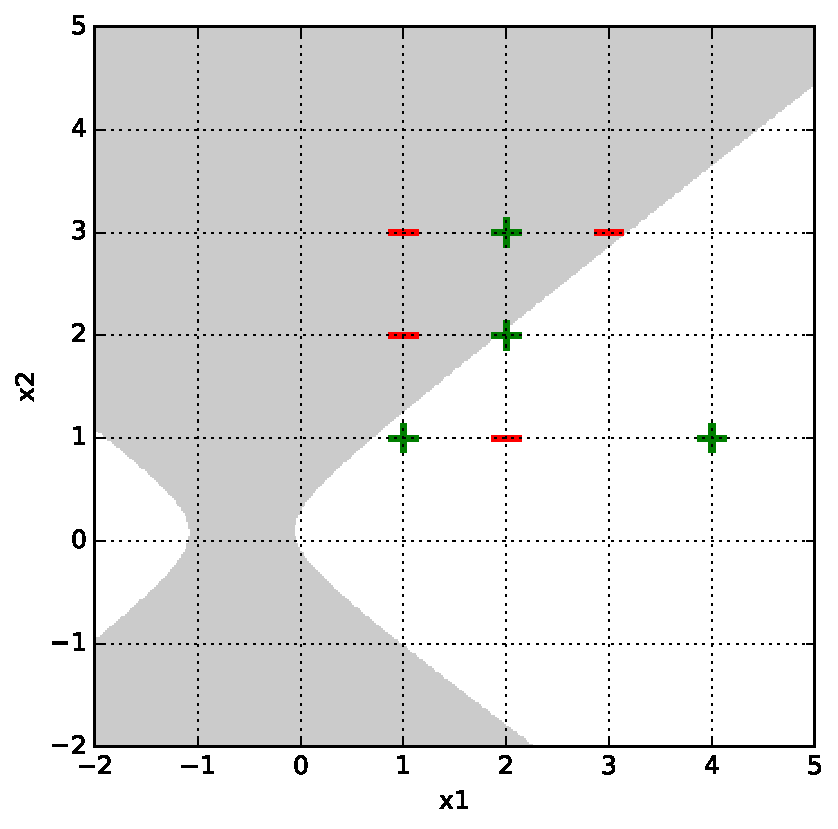
\includegraphics[width=0.48\linewidth]{figures/feature_representation_hard_order2.pdf}
    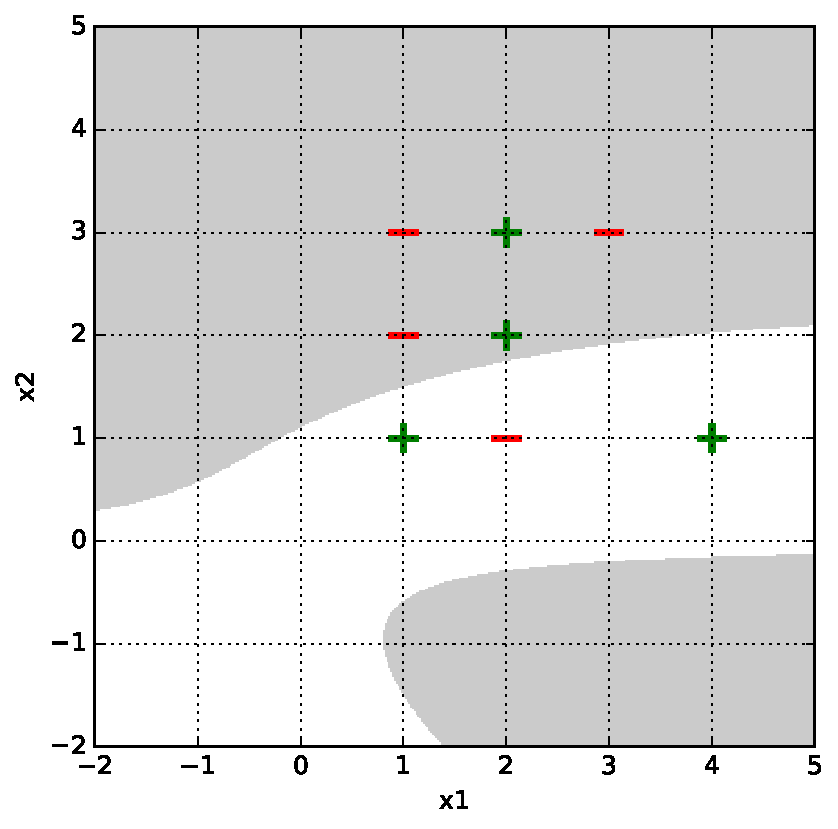
\includegraphics[width=0.48\linewidth]{figures/feature_representation_hard_order3.pdf} \\
    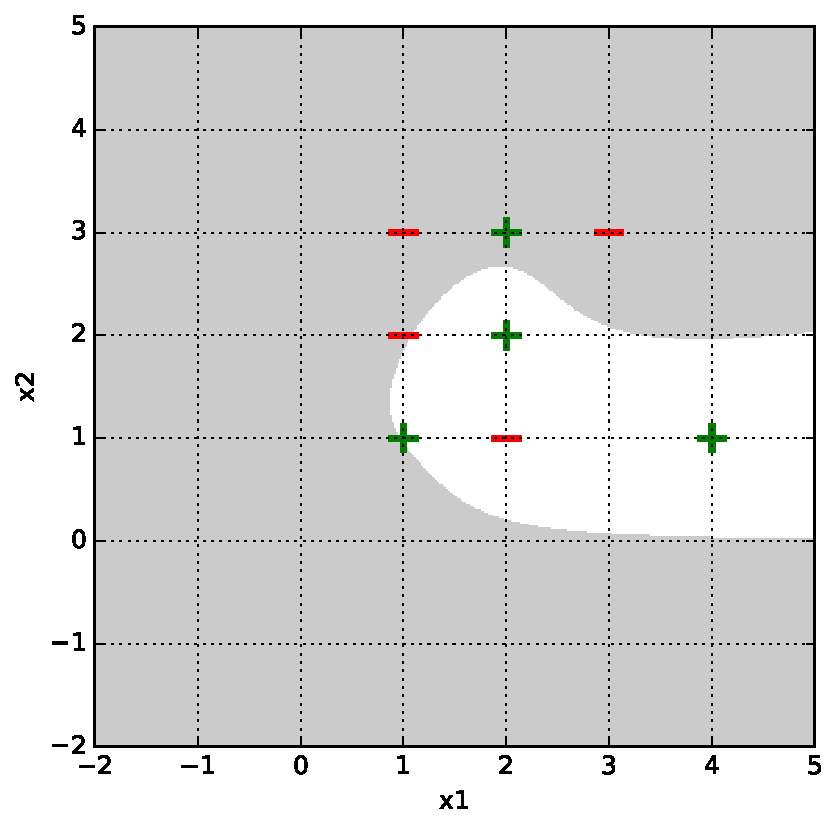
\includegraphics[width=0.48\linewidth]{figures/feature_representation_hard_order4.pdf}
    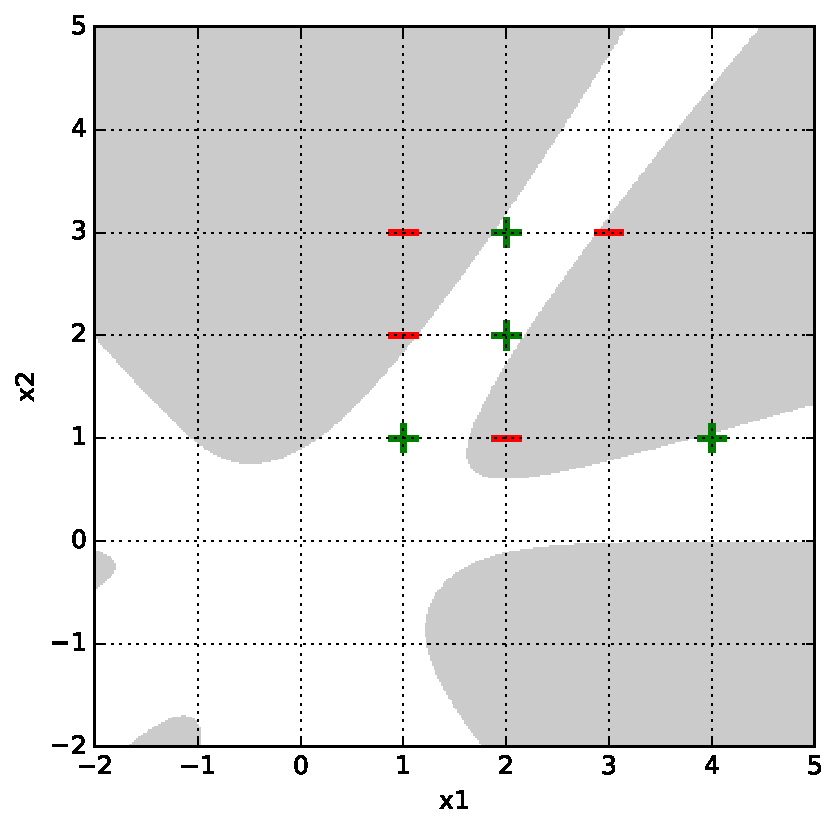
\includegraphics[width=0.48\linewidth]{figures/feature_representation_hard_order5.pdf}
  \end{center}
\end{examplebox}

\question{
Percy Eptron has a domain with four numeric input features, $(x_1,
  \ldots, x_4)$.  He decides to use a representation of the form
\[\phi(x) = {\rm PolyBasis}((x_1, x_2), 3) ^\frown
{\rm PolyBasis}((x_3, x_4), 3)\]
where $a^\frown b$ means the vector $a$ concatenated with the vector
$b$.   What is the dimension of Percy's representation?  Under what
assumptions about the original features is this a reasonable choice?
}


%%%%%%%%%%%%%%%%%%%%%%%%%%%%%%%%%%%%%%%%%%%%%%%%%%%%%%%%%%%%%%%%%%%%%%%%%%%%%

\subsection{Radial basis functions}
\index{basis functions!radial basis}
Another cool idea is to use {\em the training data itself} to
construct a feature space.  The idea works as follows.  For any
particular point $p$ in the input space $\mathcal{X}$, we can construct a feature
$f_p$ which takes any element $x \in \mathcal{X}$ and returns a
scalar value that is related to how far $x$ is from the $p$ we started
with.

Let's start with the basic case, in which $\mathcal{X} = \R^d$.  Then
we can define
\[f_p(x) = e^{-\beta\norm{p - x}^2}\;\;.\]
This function is maximized when $p = x$ and decreases exponentially as
$x$ becomes more distant from $p$.

The parameter $\beta$ governs how
quickly the feature value decays as we move away from the center point
$p$.  For large values of $\beta$, the $f_p$ values are nearly 0
almost everywhere except right near $p$;  for small values of $\beta$,
the features have a high value over a larger part of the space.

\question{What is $f_p(p)$?}

Now, given a dataset $\data$ containing $n$ points, we can make a
feature transformation $\phi$ that maps points in our original
space, $\R^d$, into points in a new space, $\R^n$.  It is defined as
follows:
\[\phi(x) = [f_{\ex{x}{1}}(x), f_{\ex{x}{2}}(x), \ldots,
  f_{\ex{x}{n}}(x)]^T\;\;.\]
So, we represent a new datapoint $x$ in terms of how far it is from
each of the datapoints in our training set.

This idea can be generalized in several ways and is the fundamental
concept underlying {\em kernel methods}\index{kernel methods}, that
you should read about some time. This idea of describing objects in
terms of their similarity to a set of reference objects is very
powerful and can be applied to cases where $\mathcal{X}$ is not a
simple vector space, but where the inputs are graphs or strings or
other types of objects, as long as there is a distance metric defined
on it.

%TODO:  Add rbf logistic regression plots

\section{Hand-constructing features for real domains}

\label{handBuiltFeatures}
In many machine-learning applications, we are given descriptions of
the inputs with many different types of attributes, including numbers,
words, and discrete features.  An important factor in the success of
an ML application is the way that the features are chosen to be encoded
by the human who is framing the learning problem.

\subsection{Discrete features}
Getting a good encoding of discrete features is particularly
important.  You want to create ``opportunities'' for the ML system to
find the underlying regularities.  Although there are machine-learning
methods that have special mechanisms for handling discrete inputs,
most of
the methods we consider in this class will assume the input vectors
$x$ are in $\R^d$.  So, we have to figure out some reasonable
strategies for turning discrete values into (vectors of) real numbers.

We'll start by listing some encoding strategies, and then work through
some examples. Let's assume we have some feature in our raw data that
can take on one of $k$ discrete values.
\begin{itemize}
  \item{\bf Numeric:}  Assign each of these values a number, say $1.0/k,
          2.0/k, \ldots, 1.0$.  We might want to then do some further processing, as
        described in Section~\ref{realFeatures}.  This is a sensible
        strategy {\em only} when the discrete values really do signify some
        sort of numeric quantity, so that these numerical values are meaningful.\index{hand-built features!numeric}

  \item{\bf Thermometer code:}  If your discrete values have a natural
        ordering, from $1, \ldots, k$, but not a natural mapping into real
        numbers, a good strategy is to use a vector of length $k$ binary
        variables, where we convert discrete input value $0 < j \leq k$ into
        a vector in which the first $j$ values are $1.0$ and the rest are
        $0.0$.  This does not necessarily imply anything about the spacing
        or numerical quantities of the inputs, but does convey something
        about ordering.\index{hand-built features!thermometer}

  \item{\bf Factored code:}  If your discrete values can sensibly be
        decomposed into two parts (say the ``maker'' and ``model'' of a car),
        then it's best to treat those as two separate features, and choose
        an appropriate encoding of each one from this list.\index{hand-built features!factored}

  \item{\bf One-hot code:}  If there is no obvious numeric, ordering, or
        factorial structure, then the best strategy is to use a vector of
        length $k$, where we convert discrete input value $0 < j \leq k$
        into a vector in which all values are $0.0$, except for the $j$th,
        which is $1.0$.\index{hand-built features!one-hot}

  \item{\bf Binary code:} It might be tempting for the computer
        scientists among us to use some binary code, which would let us
        represent $k$ values using a vector of length $\log k$.  {\em This
            is a bad idea!}  Decoding a binary code takes a lot of work, and
        by encoding your inputs this way, you'd be forcing your system to
          {\em learn} the decoding algorithm.\index{hand-built features!binary code}
\end{itemize}

As an example, imagine that we want to encode blood types, that are
drawn from the set $\{A+, A-, B+, B-, AB+, AB-, O+, O-\}$.  There is
no obvious linear numeric scaling or even ordering to this set.  But
there is a reasonable {\em factoring}, into two features: $\{A, B, AB,
  O\}$ and $\{+, -\}$.  And, in fact, we can further reasonably factor
the first group into $\{A, {\rm not}A\}$, $\{B, {\rm not}B\}$.\note{It
  is sensible (according to Wikipedia!) to treat $O$ as having neither
  feature $A$ nor feature $B$.}  So, here are two plausible encodings
of the whole set:
\begin{itemize}
  \item Use a 6-D vector, with two components of the vector each encoding the
        corresponding factor using a one-hot encoding.
  \item Use a 3-D vector, with one dimension for each factor, encoding
        its presence as $1.0$ and absence as $-1.0$ (this is sometimes
        better than $0.0$).  In this case, $AB+$ would be $[1.0, 1.0, 1.0]^T$
        and $O-$ would be $[-1.0, -1.0, -1.0]^T$.
\end{itemize}
\question{How would you encode $A+$ in both of these approaches?}

\subsection{Text}
The problem of taking a text (such as a tweet or a product review, or
even this document!) and encoding it as an input for a
machine-learning algorithm is interesting and complicated.  Much later
in the class, we'll study sequential input models, where, rather than
having to encode a text as a fixed-length feature vector, we feed it
into a hypothesis word by word (or even character by character!).

There are some simple encodings that work well for basic
applications.  One of them is the {\em bag of words} ({\sc bow})
model. \index{hand-built features!text encoding} The idea is to let $d$ be the number of words in our
vocabulary (either computed from the training set or some other body
of text or dictionary).  We will then make a binary vector (with
values $1.0$ and $0.0$) of length $d$, where element $j$ has value
$1.0$ if word $j$ occurs in the document, and $0.0$ otherwise.

\subsection{Numeric values}
\label{realFeatures}
If some feature is already encoded as a numeric value (heart rate,
stock price, distance, etc.) then we should generally keep it as a
numeric value.   An exception might be a situation in which we know
there are natural ``breakpoints'' in the semantics:  for example,
encoding someone's age in the US, we might make an explicit
distinction between under and over 18 (or 21), depending on what kind
of thing we are trying to predict.   It might make sense to divide
into discrete bins (possibly spacing them closer together for the very
young) and to use a one-hot encoding for some sorts of medical situations
in which we don't expect a linear (or even monotonic) relationship
between age and some physiological features.

If we choose to leave a feature as numeric, it is typically useful to
  {\em scale} it, so that it tends to be in the range $[-1, +1]$.
Without performing this transformation, if we have one feature with
much larger values than another, it will take the learning algorithm a
lot of work to find parameters that can put them on an equal basis.
We could also perform a more involved scaling/transformation
$\phi(x) = \dfrac{x - \overline{x}}{\sigma}$, where $\overline{x}$
is the average of the $\ex{x}{i}$, and $\sigma$ is the standard deviation of
the $\ex{x}{i}$.  The resulting feature values will have mean $0$ and
standard deviation $1$.   This transformation is sometimes called {\em
    standardizing} a variable \note{Such standard variables are often known as
  ``z-scores,'' for example, in the social sciences.}.

Then, of course, we might apply a higher-order polynomial-basis
transformation to one or more groups of numeric features.

\question{
  Consider using a polynomial basis of order $k$ as a feature
  transformation $\phi$ on our data.  Would increasing $k$ tend to
  increase or decrease structural error?  What about estimation error?
}



%%% Local Variables:
%%% mode: latex
%%% TeX-master: "top"
%%% End:

\chapter{Neural Networks}
\label{chap-neural_networks}
You've probably been
hearing a lot about ``neural networks.''   Now that we have several
useful machine-learning concepts (hypothesis classes, classification,
regression,  gradient descent, regularization, etc.) we are
well equipped to understand neural networks in detail.

This is, in some sense, the ``third wave'' of neural nets.  The basic
idea is founded on the 1943 model of neurons of McCulloch and Pitts
and the learning ideas of Hebb.  There was a great deal of excitement, but
not a lot of practical success:  there were good training methods
(e.g., perceptron) for linear functions, and interesting examples of
non-linear functions, but no good way to train non-linear functions
from data.   Interest died out for a while,  but was re-kindled in the
1980s when several people \note{As with many good ideas in science,
  the basic idea for how to train non-linear neural networks with
  gradient descent was independently developed by more than one
  researcher.} came up with a way to train neural networks with
``back-propagation,'' which is a particular style of implementing
gradient descent, that we will study here.  By the mid-90s, the
enthusiasm waned again, because although we could train non-linear
networks, the training tended to be slow and was plagued by a problem
of getting stuck in local optima.   Support vector machines ({\sc svm}s)
that use regularization of high-dimensional hypotheses by seeking to maximize
the margin, and kernel methods that are an efficient and beautiful way of
using feature transformations to non-linearly transform data into a
higher-dimensional space, provided reliable learning methods with
guaranteed convergence and no local optima.

However, during the {\sc svm} enthusiasm, several groups kept working
on neural networks, and their work, in combination with an increase in
available data and computation, has made them rise again.  They have
become much more reliable and capable, and are now the method of
choice in many applications.   There are many, many \note{The number
  increases daily, as may be seen on {\tt arxiv.org}.} variations of
neural networks, which we can't even begin to survey.  We will study
the core ``feed-forward'' networks with ``back-propagation''
training, and then, in later chapters, address some of the major
advances beyond this core.

We can view neural networks from several different perspectives:
\begin{description}
  \item{\bf View 1}: An application of stochastic gradient descent for
        classification and regression with a potentially very rich
        hypothesis class.
  \item{\bf View 2}: A brain-inspired network of neuron-like computing
        elements that learn distributed representations.
  \item{\bf View 3}: A method for building applications that make
        predictions based on huge amounts of data in very complex domains.
\end{description}

We will mostly take view 1, with the understanding that the techniques
we develop will enable the applications in view 3.  View 2 was a major
motivation for the early development of neural networks, but the
techniques we will study do not \note{Some prominent
  researchers are, in fact, working hard to find analogues of these methods in
  the brain.} seem to actually account for the biological learning
processes in brains.

\section{Basic element}
The basic element of a neural network is a ``neuron,'' pictured
schematically below.  We will also sometimes refer to a
neuron as a ``unit'' or ``node.'' \index{neuron}
\begin{center}
  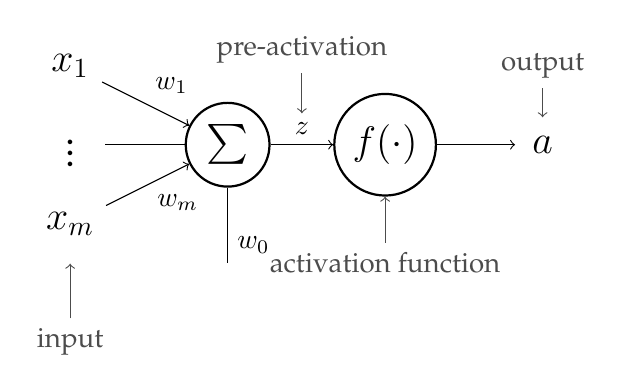
\begin{tikzpicture}[main node/.style={thick,circle,font=\Large}]
    \node[main node,draw](sum) at (0,0) {$\sum$};
    \node[main node](x1) at (-2,1) {$x_1$};
    \node[main node](dots) at (-2,0) {$\vdots$};
    \node[main node](xm) at (-2,-1) {$x_m$};
    \coordinate (w0) at (0,-1.5);
    \node[main node, draw] (f) at (2,0) {$f(\cdot)$};
    \node[main node] (y) at (4,0) {$a$};

    \draw[->, above right] (x1) -- node {$w_1$} (sum);
    \draw (dots) -- node {} (sum);
    \draw[->, below right] (xm) -- node {$w_m$} (sum);
    \draw[above right] (w0) node {$w_0$} --  (sum) ;
    \draw[->, above] (sum) -- node (z) {$z$} (f);
    \draw[->, above] (f) -- (y);

    \node[black!70] (inp) at ($(xm) + (0,-1.5)$) {input};
    \node[black!70] (pre) at ($(z) + (0,1)$) {pre-activation};
    \node[black!70] (out) at ($(y) + (0,1)$) {output};
    \node[black!70] (act) at ($(f) - (0,1.5)$) {activation function};

    \draw[->,black!70] (inp) -- (xm);
    \draw[->,black!70] (pre) -- (z);
    \draw[->,black!70] (out) -- (y);
    \draw[->,black!70] (act) -- (f);
  \end{tikzpicture}
\end{center}

It is a non-linear function of an input vector  $x \in \R^m$ \note{Sorry
  for changing our notation here.  We were using $d$ as the dimension
  of the input, but we are trying to be consistent here with many
  other accounts of neural  networks.  It is impossible to be
  consistent with all of them though---there are many different ways
  of telling this story.} to a single output value $a \in \R$.  It is
parameterized by a vector of {\em weights} $(w_1, \ldots, w_m) \in
  \R^m$ and an {\em offset} \note{This

  should remind you of our $\theta$ and $\theta_0$ for linear models.} or {\em threshold} $w_0 \in \R$. In order for the neuron to be non-linear, we also specify an {\em
    activation function} $f : \R \rightarrow \R$, which can be the
identity ($f(x) = x$, in that case the neuron is a linear function of $x$), but can also be any other function, though we
will only be able to work with it if it is differentiable.

The function represented by the neuron is expressed as:
\[a = f(z) = f\left(\left(\sum_{j=1}^m x_jw_j\right) + w_0\right) = f(w^Tx + w_0)\;\;.\]

Before thinking about a whole network, we can consider how to train a
single unit. Given a loss function $\mathcal{L}(\text{guess}, \text{actual})$
and a dataset $\{(\ex{x}{1}, \ex{y}{1}), \ldots,
  (\ex{x}{n},\ex{y}{n})\}$, we can
do (stochastic) gradient descent, adjusting the weights
$w, w_0$ to minimize
\[J(w, w_0) = \sum_{i} \mathcal{L}\left(\text{NN}(\ex{x}{i}; w, w_0), \ex{y}{i}\right)\;,\]
where $\text{NN}$ is the output of our single-unit neural net for a given input.

We have already studied two special cases of the neuron:
linear logistic classifiers (LLCs) with NLL loss and regressors with
quadratic loss! The activation function for the LLC is $f(x) =
  \sigma(x)$ and for linear regression it is simply $f(x) = x$.
\question{
  Just for a single neuron, imagine for some reason, that we decide to
  use activation function $f(z) = e^z$ and loss function $\mathcal{L}(\text{guess}, \text{actual}) = (\text{guess} - \text{actual})^2$.  Derive a gradient descent update for $w$ and $w_0$.
}
\section{Networks}
Now, we'll put multiple neurons together into a {\em network}.  A
neural network \index{neural network}in general takes in an input $x \in \R^m$ and generates
an output $a \in \R^n$.  It is constructed out of multiple neurons;
the inputs of each neuron might be elements of $x$ and/or outputs of
other neurons.   The outputs are generated by $n$ {\em output units}.  \index{neural network!output units}

In this chapter, we will only consider {\it feed-forward} networks\index{neural network!feed-forward network}.  In
a feed-forward network, you can think of the network as defining a
function-call graph that is {\em acyclic}:  that is, the input to a
neuron can never depend on that neuron's output.  Data flows one way,
from the inputs to the outputs, and the function computed by the
network is just a composition of the functions computed by the
individual neurons.

Although the graph structure of a feed-forward neural network can really be
anything (as long as it satisfies the feed-forward constraint), for
simplicity in software and analysis, we usually organize them into
  {\em layers}\index{neural network!layers}.   A layer is a group of neurons that are essentially
``in parallel'':  their inputs are outputs of neurons in the previous
layer, and their outputs are the input to the neurons in the next
layer.   We'll start by describing a single layer, and then go on to
the case of multiple layers.

\subsection{Single layer}
A {\em layer} is a set of units that, as we have just described, are
not connected to each other. The layer is called
  {\em fully connected}\index{neural network!fully connected} if, as in the diagram below, 
  all of the inputs
% the inputs to each unit in the layer are the same 
(i.e., $x_1, x_2, \ldots x_m$ in this
case) are connected to every unit in the layer.  A layer has input $x \in \R^m$ and output (also known as
  {\em activation}) $a \in \R^n$.

\begin{center}
  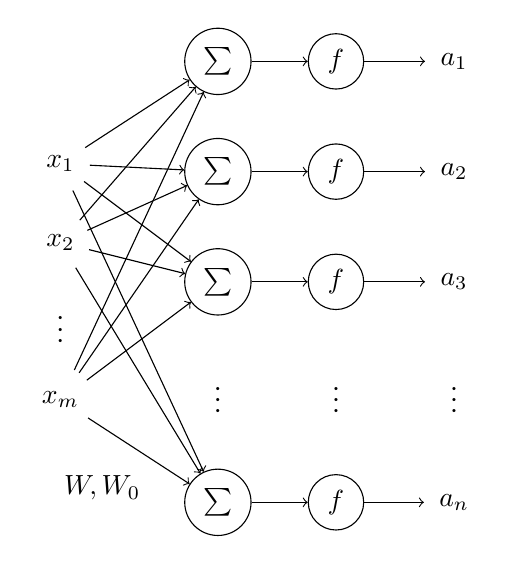
\begin{tikzpicture}[main node/.style={circle}]
    \coordinate (soff) at (0,1.4);
    \node[main node,draw](s1) at ($2*(soff)$) {$\sum$};
    \node[main node,draw](s2) at (soff) {$\sum$};
    \node[main node,draw](s3) at (0,0) {$\sum$};
    \node[main node](sdots) at ($(0,0)-(soff)$) {$\vdots$};
    \node[main node,draw](sn) at ($(0,0)-2*(soff)$) {$\sum$};

    % inputs
    \coordinate (x) at (-2,0);
    \coordinate (xoff) at (0,1);
    \node[main node](x1) at ($(x) + 1.5*(xoff)$) {$x_1$};
    \node[main node](x2) at ($(x) + .5*(xoff)$) {$x_2$};
    \node[main node](xdots) at ($(x) - .5*(xoff)$) {$\vdots$};
    \node[main node](xm) at ($(x) - 1.5*(xoff)$) {$x_m$};

    % activations
    \coordinate (foff) at (1.5,0);
    \node[main node, draw](f1) at ($(s1) + (foff)$) {$f$};
    \node[main node, draw](f2) at ($(s2) + (foff)$) {$f$};
    \node[main node, draw](f3) at ($(s3) + (foff)$) {$f$};
    \node[main node] at ($(sdots) + (foff)$) {$\vdots$};
    \node[main node, draw](fn) at ($(sn) + (foff)$) {$f$};

    % outputs
    \node[main node](y1) at ($(s1) + 2*(foff)$) {$a_1$};
    \node[main node](y2) at ($(s2) + 2*(foff)$) {$a_2$};
    \node[main node](y3) at ($(s3) + 2*(foff)$) {$a_3$};
    \node[main node] at ($(sdots) + 2*(foff)$) {$\vdots$};
    \node[main node](yn) at ($(sn) + 2*(foff)$) {$a_n$};

    % arrows
    \foreach \b in {(s1), (s2), (s3), (sn)}
    \foreach \a in {(x1), (x2), (xm)}
    \draw[->] \a -- \b;
    \foreach \x/\y/\z in {(s1)/(f1)/(y1), (s2)/(f2)/(y2),
        (s3)/(f3)/(y3), (sn)/(fn)/(yn)}{
        \draw[->] \x -- \y;
        \draw[->] \y -- \z;
      }
    %\foreach \x in {(s1), (s2), (s3), (sn)}
    %  \draw \x -- +(0,-.65);
    \node[main node, ,below left] (weights) at ($(xm)!0.5!(sn)$)
    {$W,W_0$};
  \end{tikzpicture}
\end{center}
Since each unit has a vector of weights and a single offset, we can
think of the weights of the whole layer as a matrix, $W$, and the
collection of  all the offsets as a vector $W_0$.
If we have $m$ inputs, $n$ units, and $n$ outputs, then
\begin{itemize}
  \item $W$ is an $m\times n$ matrix,
  \item $W_0$ is an $n \times 1$ column vector,
  \item $X$, the input, is an $m \times 1$ column vector,
  \item $Z = W^T X + W_0$, the {\em pre-activation}, is an $n \times
          1$ column vector,
  \item $A$, the {\em activation}, is an $n \times 1$ column vector,
\end{itemize}
and the output vector is
\[A = f(Z) = f(W^TX + W_0)\;\;.\]
The activation function $f$ is applied element-wise to the
pre-activation values $Z$.

% What can we do with a single layer?  We have already seen single-layer
% networks, in the form of linear separators and linear regressors.  All
% we can do with a single layer is make a linear hypothesis.~\note{We
%   have used a step or sigmoid function to transform the linear output
%   value for classification, but it's important to be clear that the
%   resulting {\em separator} is still linear.} The whole reason for
% moving to neural networks is to move in the direction of {\em
%     non-linear} hypotheses.  To do this, we will have to consider
% multiple layers, where we can view the last layer as still being a
% linear classifier or regressor, but where we interpret the previous
% layers as learning a non-linear feature transformation $\phi(x)$,
% rather than having us hand-specify it.

\subsection{Many layers}
A single neural network generally combines multiple layers, most
typically by feeding the outputs of one layer into the inputs of
another layer.

We have to start by establishing some nomenclature.  We will use $l$
to name a layer, and let $m^l$ be the number of inputs to the layer
and $n^l$ be the number of outputs from the layer.  Then, $W^l$ and
$W^l_0$ are of shape $m^l \times n^l$ and $n^l \times 1$,
respectively. Note that the input to layer $l$ is the output from
layer $l-1$, so we have $m^l= n^{l-1}$, and as a result $A^{l-1}$ is
of shape $m^l \times 1$, or equivalently $n^{l-1} \times 1$. Let $f^l$
be the activation function\index{activation function} of layer
$l$. \note{It is technically possible to have different activation
  functions within the same layer, but, again, for convenience in
  specification and implementation, we generally have the same
  activation function within a layer.}Then, the pre-activation outputs
are the $n^l \times 1$ vector
\[Z^l = {W^l}^TA^{l-1} + W^l_0\]
and the activation outputs are simply the $n^l \times 1$ vector
\[A^l = f^l(Z^l)\;\;.\]

Here's a diagram of a many-layered network, with two blocks
for each layer, one representing the linear part of the operation and
one representing the non-linear activation function.  We will use this
structural decomposition to organize our algorithmic thinking and
implementation.

\begin{center}
  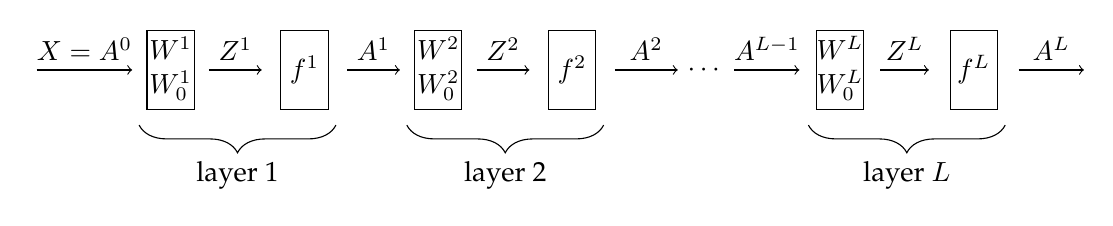
\begin{tikzpicture}
    \coordinate (x) at (0,0);
    \node[inner sep=0em] (w1) at (1.7,0)
    {\begin{tabular}{c} $W^1$ \\ $W^1_0$\end{tabular}};
    \node[inner sep=1em] (f1) at ($2*(w1)$) {$f^1$};
    \node[inner sep=0em] (w2) at ($3*(w1)$)
    {\begin{tabular}{c} $W^2$ \\ $W^2_0$\end{tabular}};
    \node[inner sep=1em] (f2) at ($4*(w1)$) {$f^2$};
    \node (dots) at ($5*(w1)$) {$\cdots$};
    \node[inner sep=0em] (wL) at ($6*(w1)$)
    {\begin{tabular}{c} $W^L$ \\ $W^L_0$\end{tabular}};
    \node[inner sep=1em] (fL) at ($7*(w1)$) {$f^L$};
    \coordinate (y) at ($8*(w1) - (.3,0)$);

    \draw[->] (x) -- node[above] {$X = A^0$} (w1);
    \draw[->] (w1) -- node[above] {$Z^1$} (f1);
    \draw[->] (f1) -- node[above] {$A^1$} (w2);
    \draw[->] (w2) -- node[above] {$Z^2$} (f2);
    \draw[->] (f2) -- node[above] {$A^2$} (dots);
    \draw[->] (dots) -- node[above] {$A^{L-1}$} (wL);
    \draw[->] (wL) -- node[above] {$Z^L$} (fL);
    \draw[->] (fL) -- node[above] {$A^L$} (y);

    \draw [decorate,decoration={brace,mirror,amplitude=10pt}]
    ($(w1) + (-.4, -.7)$) -- node[yshift=-1.8em] {layer 1}
    ($(f1) + (.4,-.7)$);
    \draw [decorate,decoration={brace,mirror,amplitude=10pt}]
    ($(w2) + (-.4, -.7)$) -- node[yshift=-1.8em] {layer 2}
    ($(f2) + (.4,-.7)$);
    \draw [decorate,decoration={brace,mirror,amplitude=10pt}]
    ($(wL) + (-.4, -.7)$) -- node[yshift=-1.8em] {layer $L$}
    ($(fL) + (.4,-.7)$);


    \foreach \point in {w1, f1, w2, f2, wL, fL}{
        \draw ($(\point) + (-.3,-.5)$) rectangle ($(\point) + (.3,.5)$);
      }
  \end{tikzpicture}
\end{center}

\section{Choices of activation function}

There are many possible choices for the activation function.  We will
start by thinking about whether it's really necessary to have an $f$
at all.

What happens if we let $f$ be the identity?  Then, in a network with
$L$ layers (we'll leave out $W_0$ for simplicity, but keeping it
wouldn't change the form of this argument),
\[A^L = {W^L}^T A^{L-1} =
    {W^L}^T {W^{L-1}}^T \cdots {W^1}^T X\;\;.\]
So, multiplying out the weight matrices, we find that
\[A^L = W^\text{total}X\;\;,\]
which is a {\em linear} function of $X$!
Having all those layers did not change the representational
capacity of the network: the non-linearity of the activation function
is crucial.
\question{Convince yourself that any function representable by any
  number of linear layers (where $f$ is the identity function) can be
  represented by a single layer.}

Now that we are convinced we need a non-linear activation, let's
examine a few common choices.
These are shown mathematically below, followed by plots of these functions.
\begin{description}
  \item{\bf Step function:} \index{activation function!step function}
        $$\text{step}(z) =
          \begin{cases}
            0 & \text{if $z<0$}  \\
            1 & \text{otherwise}
          \end{cases}$$
  \item{\bf Rectified linear unit (ReLU):} \index{activation function!ReLU}
        $$\text{ReLU}(z) =
          \begin{cases}
            0 & \text{if $z<0$}  \\
            z & \text{otherwise}
          \end{cases} = \max(0,z)$$
  \item{\bf Sigmoid function:}\index{activation function!sigmoid} Also known as a {\em logistic} function. This can sometimes
        be interpreted as probability, because for any value of $z$ the
        output is in $(0, 1)$:
        $$\sigma(z) = \frac{1}{1+e^{-z}}$$
  \item{\bf Hyperbolic tangent:}\index{activation function!hyperbolic tangent} Always in the range $(-1, 1)$:
        $$\tanh(z) = \frac{e^z - e^{-z}}{e^z + e^{-z}}$$
  \item{\bf Softmax function:}\index{activation function!softmax}
        Takes a whole vector $Z \in \R^n$ and generates as output a vector
        $A \in (0, 1)^n$ with the property that $\sum_{i = 1}^n A_i = 1$,
        which means we can interpret it as a probability distribution over $n$ items:
        \[\text{softmax}(z) =
          \begin{bmatrix}
            \exp(z_1) / \sum_{i} \exp(z_i) \\
            \vdots                         \\
            \exp(z_n) / \sum_{i} \exp(z_i)
          \end{bmatrix}\]

\end{description}

\noindent\begin{center}
  \resizebox{0.9\textwidth}{!}{%
    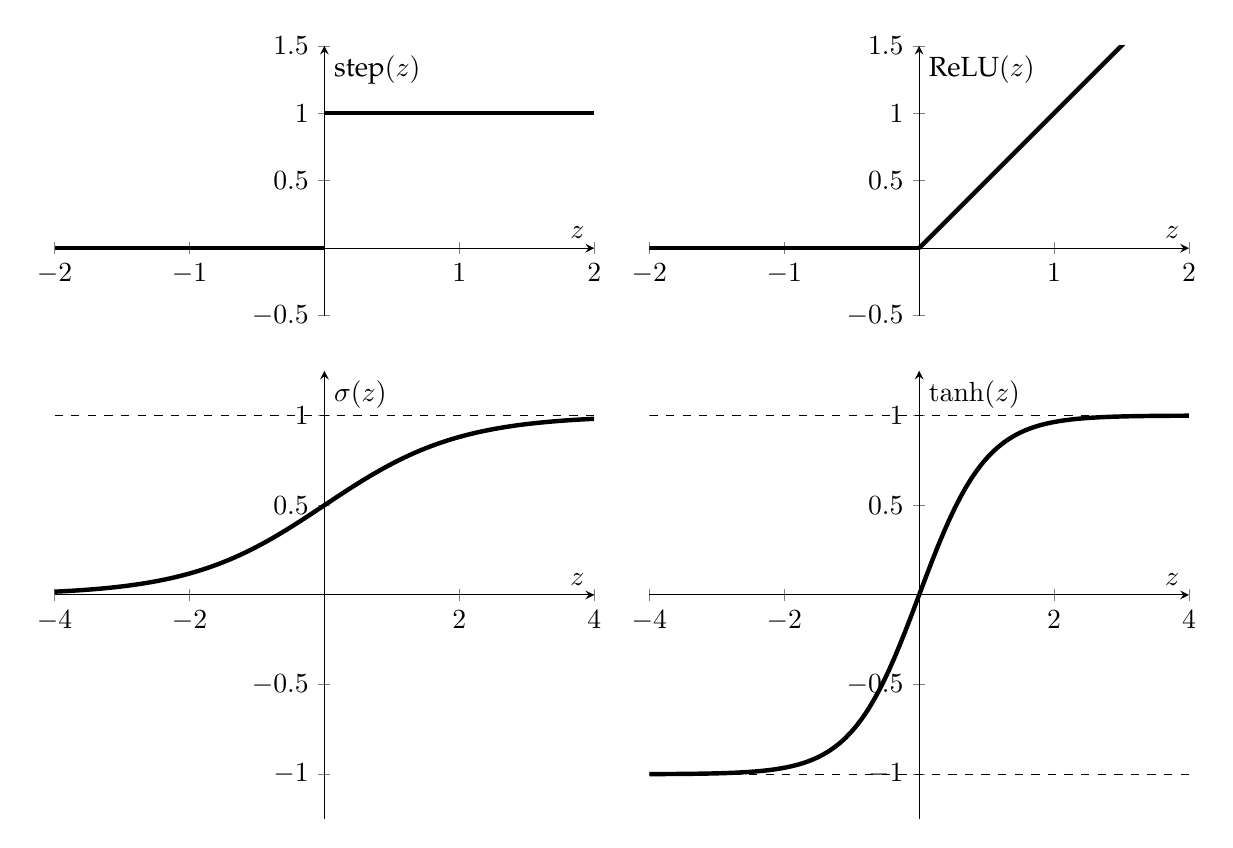
\begin{tikzpicture}%[scale=.9]
      \begin{axis}[
          name=topleft,
          axis lines=middle, axis equal image,
          xmin=-2, xmax=2,
          ymin=-.5, ymax=1.5,
          xlabel={$z$}, ylabel={$\text{step}(z)$},
        ]
        \addplot [domain=-2:0, samples=2, ultra thick] {0};
        \addplot [domain=0:2, samples=2, ultra thick] {1};
      \end{axis}

      \begin{axis}[
          name=topright,
          axis lines=middle, axis equal image,
          xmin=-2, xmax=2,
          ymin=-.5, ymax=1.5,
          xlabel={$z$}, ylabel={$\text{ReLU}(z)$},
          at = (topleft.east), anchor=west, xshift=.7cm
        ]
        \addplot [domain=-2:0, samples=2, ultra thick] {0};
        \addplot [domain=0:2, samples=2, ultra thick] {x};
      \end{axis}

      \begin{axis}[
          name=bottomleft,
          axis lines=middle, %axis equal image,
          xmin=-4, xmax=4,
          ymin=-1.25, ymax=1.25,
          xlabel={$z$}, ylabel={$\sigma(z)$},
          at = (topleft.south), anchor=north, yshift=-.7cm
        ]
        \addplot [domain=-4:4, samples=100, ultra thick] {1/(1+exp(-x))};
        \addplot [domain=-4:4, samples=2, dashed] {1};
        \addplot [domain=-4:4, samples=2, dashed] {0};
      \end{axis}

      \begin{axis}[
          name=bottomright,
          axis lines=middle, %axis equal image,
          xmin=-4, xmax=4,
          ymin=-1.25, ymax=1.25,
          xlabel={$z$}, ylabel={$\tanh(z)$},
          at = (bottomleft.east), anchor=west, xshift=.7cm
        ]
        \addplot [domain=-4:4, samples=100, ultra thick]
        {(exp(x) - exp(-x))/(exp(x) + exp(-x))};
        \addplot [domain=-4:4, samples=2, dashed] {1};
        \addplot [domain=-4:4, samples=2, dashed] {-1};
      \end{axis}
    \end{tikzpicture}
  }%
\end{center}

The original idea for neural networks involved using the {\bf step}
function as an activation, but because the derivative of the
step function is zero everywhere except at the discontinuity
(and there it is undefined), gradient-descent methods won't be useful
in finding a good setting of the weights, and so we won't
consider them further.  They have been replaced, in a sense, by the
sigmoid, ReLU, and tanh activation functions.
\question{
  Consider sigmoid, ReLU, and tanh activations.  Which one is most like
  a step function?  Is there an additional parameter you could add to a
  sigmoid that would make it be more like a step function?
}
\question{
  What is the derivative of the ReLU function?  Are there some values of
  the input for which the derivative vanishes?
}

ReLUs are especially common in internal (``hidden'') layers, 
sigmoid activations are common for the output for binary
classification, and softmax activations are common for the output for multi-class classification
(see Section~\ref{logistic} for an explanation).

\section{Loss functions and activation functions}\index{neural network!loss and activation function choices}
Different loss functions make different assumptions about the range of
values they will get as input and, as we have seen, different
activation functions will produce output values in different ranges.
When you are designing a neural network, it's important to make these
things fit together well.  In particular, we will think about matching
loss functions with the activation function in the last layer, $f^L$.
Here is a table of loss functions and activations that make sense for them:
\begin{center}
  \begin{tabular}{c c l}
    Loss       & $f^L$   & task                       \\
    \hline
    squared    & linear  & regression                 \\
    %  hinge & linear \\
    {\sc nll}  & sigmoid & binary classification             \\
    {\sc nllm} & softmax & multi-class classification
  \end{tabular}
\end{center}
We explored squared loss in Chapter~\ref{chap-regression} and ({\sc nll} and {\sc nllm}) in
Chapter~\ref{chap-classification}.

% \subsection{Two-class classification and log likelihood}
% For classification, the natural loss function is 0-1 loss, but we have
% already discussed the fact that it's very inconvenient for
% gradient-based learning because its derivative is discontinuous.

% It is nice
% and smooth, and extends nicely to multiple classes as we will see below.

% {\em Hinge loss} gives us another way, for binary classification
% problems, to make a smoother objective, penalizing the {\em margin}s
% of the labeled points relative to the separator.  The hinge loss is
% defined to be
% \[\mathcal{L}_h(\text{guess},\text{actual}) = \max(1 - \text{guess} \cdot
%   \text{actual}, 0)\;\;,\]
% when $\text{actual} \in \{+1, -1\}$.  It has the property that, if the
% sign of $\text{guess}$ is the same as the sign of $\text{actual}$ and the
% magnitude of $\text{guess}$ is greater than $1$, then the loss is 0.

% It is trying to enforce not only that the guess have the correct sign,
% but also that it should be some distance away from the separator.
% Using hinge loss, together with a squared-norm regularizer, actually
% forces the learning process to try to find a separator that has the
% maximum {\em margin} relative to the data set.  This optimization
% set-up is called a {\em support vector machine}, and was popular
% before the renaissance of neural networks and gradient descent,
% because it has a quadratic form that makes it particularly easy to
% optimize.



% Let's assume that the activation function on the output layer is a
% sigmoid and that there is a single unit in the output layer, so the
% output of the whole neural network is a scalar, $a^L$.  Because $f^L$
% is a sigmoid, we know $a^L \in [0, 1]$, and we can interpret it as the
% probability that  the input $x$ is a positive example.  Let  us
% further assume that the labels in the training data are $y \in \{0,
% 1\}$, so they can also be interpreted  as probabilities.

% We might want to pick the parameters of our network to maximize the
% probability that the network assigns the correct labels  to all the
% points.  That would be
% \begin{equation*}
%  \prod_{i = 1}^n \begin{cases} \ex{a}{i} & \text{if $\ex{y}{i} =
%     1$}  \\ 1 - \ex{a}{i} & \text{otherwise}
% \end{cases}\;\;,
% \end{equation*}
% under the assumption that our predictions are independent.  This can
% be cleverly rewritten as
% \begin{equation*}
%  \prod_{i = 1}^n {\ex{a}{i}}^{\ex{y}{i}}(1 - \ex{a}{i})^{1 - \ex{y}{i}}\;\;.
% \end{equation*}
% \question{Be sure you can see why these two expressions are  the
%   same.}

% Now, because products are kind of hard to deal with, and because the
% log function is monotonic, the $W$ that maximizes the log of this
% quantity will be the same  as the $W$ that maximizes the original, so
% we can try to maximize
% \begin{equation*}
%  \sum_{i = 1}^n {\ex{y}{i}}\log {\ex{a}{i}} + (1 - \ex{y}{i})\log(1 -
%  \ex{a}{i})\;\;,
% \end{equation*}
% which we can write in terms of a loss function
% \begin{equation*}
%  \sum_{i = 1}^n \mathcal{L}_\text{nll}(\ex{a}{i}, \ex{y}{i})
% \end{equation*}
% where $\mathcal{L}_\text{nll}$ is the {\em negative log likelihood}
% loss function:
% \begin{equation*}
% \mathcal{L}_\text{nll}(\text{guess},\text{actual}) =
% -\left(\text{actual}\cdot \log (\text{guess}) + (1 - \text{actual})\cdot\log (1 -
%   \text{guess})\right) \;\;.
% \end{equation*}
% This loss function is also sometimes referred to as the {\em log loss}
% or {\em cross entropy}. \note{You can use any base for the logarithm
%   and it won't make any real difference.  If we ask you for numbers,
%   use log base $e$.}

% \subsection{Multi-class classification and log likelihood}
% We can extend the idea of NLL directly to multi-class classification with
% $K$ classes, where the training label is represented with the one-hot
% vector
% $y=\begin{bmatrix} y_1,  \ldots, y_K \end{bmatrix}^T$, where $y_k=1$
% if the example is of class $k$. Assume that our network uses {\em
%   softmax} as the activation function in the last layer, so that the
% output is
% $a=\begin{bmatrix} a_1, \ldots, a_K
% \end{bmatrix}^T$, which represents a probability distribution over
% the $K$ possible classes. Then, the probability that our network
% predicts the correct class for this example is
% $\prod_{k=1}^K a_k^{y_k}$ and the log of the probability that it is
% correct is $\sum_{k=1}^K y_k \log a_k$, so
% \[
% \mathcal{L}_\text{nllm}(\text{guess},\text{actual}) =
% - \sum_{k=1}^K \text{actual}_k \cdot \log(\text{guess}_k) \;\;.
% \]
% We'll call this {\sc nllm} for {\em negative log likelihood
%   multiclass.}
% \question{Show that $L_\text{nllm}$ for  $K = 2$ is the same as
%   $L_\text{nll}$. }

%%%%%%%%%%%%%%%%%%%%%%%%%%%%%%%%%%%%%%%%

\section{Error back-propagation}
We will train neural networks using gradient descent methods.\index{gradient descent!applied to neural network training}  It's
possible to use {\em batch} gradient descent, in which we sum up the
gradient over all the points (as in Section~\ref{sec-gd} of
chapter~\ref{chap-gradient}) or
stochastic gradient descent ({\sc sgd}), in which we take a small step with
respect to the gradient considering a single point at a time (as in
Section~\ref{sec-sgd} of Chapter~\ref{chap-gradient}).

Our notation is going to get pretty hairy pretty quickly.  To keep it
as simple as we can, we'll focus on computing the contribution of one
data point $\ex{x}{i}$ to the gradient of the loss with respect to the
weights, for {\sc sgd}; you can simply sum up these gradients over all
the data points if you wish to do batch descent.

So, to do {\sc sgd} for a training example $(x, y)$, we need to
compute $\nabla_W \mathcal{L}(\text{NN}(x;W),y)$,
where $W$ represents all weights $W^l, W_0^l$ in all the layers $l =
  (1, \ldots, L)$. This seems terrifying,
but is actually quite easy to do using the chain rule.
\note{Remember the chain rule!  If $a = f(b)$ and $b = g(c)$, so that\\
  $a = f(g(c))$, then \\$\frac{d a}{d c} = \frac{d a}{d b} \cdot \frac{d
    b}{d c} = f'(b) g'(c) = f'(g(c)) g'(c)$.}

Remember that we are always computing the gradient of the loss
function {\em with respect to the weights} for a particular value of
$(x,  y)$.  That tells us how much we want to change the weights, in
order to reduce the loss incurred on this particular training example.

\subsection{First, suppose everything is one-dimensional}

To get some intuition for how these derivations work, we'll first suppose everything in our neural network is one-dimensional.
In particular, we'll assume there are $m^l = 1$ inputs and $n^l = 1$ outputs at every layer. So layer $l$ looks like:
\[
  a^l = f^l(z^l), \quad z^l = w^l a^{l-1} + w^l_0.
\]
In the equation above, we're using the lowercase letters $a^l, z^l, w^l, a^{l-1}, w^l_0$ to emphasize that all of these quantities are scalars just for the moment. We'll look at the more general matrix case below.

To use {\sc sgd}, then, we want \note{Check your understanding: why do we need exactly these quantities for SGD?} to compute $\partial \mathcal{L}(\text{NN}(x;W),y) / \partial w^l$ and $\partial \mathcal{L}(\text{NN}(x;W),y) / \partial w_0^l$ for each layer $l$ and each data point $(x,y)$. Below we'll write ``loss'' as an abbreviation for $\mathcal{L}(\text{NN}(x;W),y)$. Then our first quantity of interest is $\partial \text{loss} / \partial w^l$. The chain rule gives us the following.
First, let's look at the case $l=L$:
\begin{eqnarray*}
  \frac{ \partial \text{loss} }{ \partial w^L }
  &=& \frac{ \partial \text{loss} }{ \partial a^L }
  \cdot \frac{ \partial a^L }{ \partial z^L }
  \cdot \frac{ \partial z^L }{ \partial w^L } \\
  &=& \frac{ \partial \text{loss} }{ \partial a^L } \cdot (f^L)'(z^L) \cdot a^{L-1}.
\end{eqnarray*}
Now we can look at the case of general $l$:
\begin{eqnarray*}
  \frac{ \partial \text{loss} }{ \partial w^l }
  &=& \frac{ \partial \text{loss} }{ \partial a^L }
  \cdot \frac{ \partial a^L }{ \partial z^L }
  \cdot \frac{ \partial z^L }{ \partial a^{L-1} }
  \cdot \frac{ \partial a^{L-1} }{ \partial z^{L-1} }
  \cdots
  %\frac{ \partial a^{l+1} }{ \partial z^{l+1} }
  \frac{ \partial z^{l+1} }{ \partial a^{l} }
  \cdot \frac{ \partial a^{l} }{ \partial z^l }
  \cdot \frac{ \partial z^l }{ \partial w^l } \\
  &=& \frac{ \partial \text{loss} }{ \partial a^L } \cdot (f^L)'(z^L) \cdot w^L
  \cdot (f^{L-1})'(z^{L-1})
  \cdots
  %\cdot (f^{l+1})'(z^{l+1})
  \cdot w^{l+1}
  \cdot (f^{l})'(z^{l})
  \cdot a^{l-1} \\
  &=& \frac{ \partial \text{loss} }{ \partial z^l } \cdot a^{l-1}.
\end{eqnarray*}

Note that every multiplication above is scalar multiplication because every term in every product above is a scalar. And though we solved for all the other terms in the product, we haven't solved for $\partial \text{loss} / \partial a^L$ because the derivative will depend on which loss function you choose. Once you choose a loss function though, you should be able to compute this derivative.

\question{Suppose you choose squared loss. What is $\partial \text{loss} / \partial a^L$?}

\question{Check the derivations above yourself. You should use the chain rule and also solve for the individual derivatives that arise in the chain rule.}

\question{Check that the the final layer ($l=L$) case is a special case of the general layer $l$ case above.}

\question{Derive $\partial \mathcal{L}(\text{NN}(x;W),y) / \partial w_0^l$ for yourself, for both the final layer ($l=L$) and general $l$.}

\question{Does the $L=1$ case remind you of anything from earlier in this course?}

\question{Write out the full SGD algorithm for this neural network.}

It's pretty typical to run the chain rule from left to right like we did above. But, for where we're going next, it will be useful to notice that it's completely equivalent to write it in the other direction. So we can rewrite our result from above as follows:
\begin{eqnarray}
  \label{eq:gradloss_oned}
  \frac{ \partial \text{loss} }{ \partial w^l }
  &=& a^{l-1} \cdot \frac{ \partial \text{loss} }{ \partial z^l } \\
  \label{eq:gradz_intermediate_oned}
  \frac{ \partial \text{loss} }{ \partial z^l }
  &=& \frac{ \partial a^{l} }{ \partial z^l }
  \cdot \frac{ \partial z^{l+1} }{ \partial a^{l} }
  \cdots
  \frac{ \partial a^{L-1} }{ \partial z^{L-1} }
  \cdot \frac{ \partial z^L }{ \partial a^{L-1} }
  \cdot \frac{ \partial a^L }{ \partial z^L }
  \cdot \frac{ \partial \text{loss} }{ \partial a^L } \\
  \label{eq:gradz_oned}
  &=& \frac{ \partial a^{l} }{ \partial z^l } \cdot w^{l+1}
  \cdots
  \frac{ \partial a^{L-1} }{ \partial z^{L-1} } \cdot w^L \cdot \frac{ \partial a^L }{ \partial z^L }
  \cdot \frac{ \partial \text{loss} }{ \partial a^L }.
\end{eqnarray}


\subsection{The general case}

Next we're going to do everything that we did above, but this time we'll allow any number of inputs $m^l$ and outputs $n^l$ at every layer. First, we'll tell you the results that correspond to our derivations above. Then we'll talk about why they make sense. And finally we'll derive them carefully.

OK, let's start with the results! Again, below we'll be using ``loss'' as an abbreviation for $\mathcal{L}(\text{NN}(x;W),y)$. Then,
\begin{eqnarray}
  \label{eq:gradloss}
  \underbrace{\frac{\partial \text{loss}}{\partial W^l}}_{m^l \times n^l}
  &=&
  \underbrace{A^{l-1}}_{m^l \times 1} \;
  \underbrace{\left(\frac{\partial \text{loss}}{\partial
      Z^l}\right)^T}_{1 \times n^l} \\
  %
  \label{eq:gradz_intermediate}
  \frac{\partial \text{loss}}{\partial Z^l}
  &=& \frac{\partial A^l}{\partial Z^l}
  %%\cdot \frac{\partial Z^l}{ \partial A^{l+1}}
  \cdot \frac{\partial Z^{l+1}}{ \partial A^l}
  %\cdot \frac{\partial A^{l+1}}{\partial Z^{l+1}}
  \cdots
  %\cdot \frac{\partial Z^{L-1}}{\partial A^{L-2}}
  \cdot \frac{\partial A^{L-1}}{\partial Z^{L-1}}
  \cdot \frac{\partial Z^{L}}{\partial A^{L-1}}
  \cdot \frac{\partial A^{L}}{\partial Z^{L}}
  \cdot \frac{\partial \text{loss}}{\partial A^L}
  \\
  \label{eq:gradz}
  &=& \frac{\partial A^l}{\partial Z^l}
  \cdot W^{l+1}
  % \cdot W^l
  %\cdot \frac{\partial A^{l+1}}{\partial Z^{l+1}}
  \cdots
  %W^{L-1}
  \cdot \frac{\partial A^{L-1}}{\partial Z^{L-1}}
  \cdot W^{L}
  \cdot \frac{\partial A^{L}}{\partial Z^{L}}
  \cdot \frac{\partial \text{loss}}{\partial A^L} \; .
\end{eqnarray}

First, compare each equation to its one-dimensional counterpart, and make sure you see the similarities.
That is, compare the general weight derivatives in Eq.~\ref{eq:gradloss} to the one-dimensional case in Eq.~\ref{eq:gradloss_oned}. Compare the intermediate derivative of loss with respect to the pre-activations $Z^l$ in Eq.~\ref{eq:gradz_intermediate} to the one-dimensional case in Eq.~\ref{eq:gradz_intermediate_oned}. And finally compare the version where we've substituted in some of the derivatives in Eq.~\ref{eq:gradz} to Eq.~\ref{eq:gradz_oned}. Hopefully you see how the forms are very analogous. But in the matrix case, we now have to be careful about the matrix dimensions. We'll check these matrix dimensions below.

Let's start by talking through each of the terms in the matrix version of these equations. Recall that loss is a scalar, and $W^l$ is a matrix of size $m^l \times n^l$. You can read about the conventions in the course for derivatives starting in this chapter in Appendix~\ref{app:matrix_deriv}. By these conventions (not the only possible conventions!), we have that $\partial \text{loss} / \partial W^l$ will be a matrix of size $m^l \times n^l$ whose $(i,j)$ entry is the scalar $\partial \text{loss} / \partial W^l_{i,j}$. In some sense, we're just doing a bunch of traditional scalar derivatives, and the matrix notation lets us write them all simultaneously and succinctly. In particular, for SGD, we need to find the derivative of the loss with respect to every scalar component of the weights because these are our model's parameters and therefore are the things we want to update in SGD.

The next quantity we see in Eq.~\ref{eq:gradloss} is $A^{l-1}$, which we recall has size $m^l \times 1$ (or equivalently $n^{l-1} \times 1$ since it represents the outputs of the $l-1$ layer). Finally, we see $\partial \text{loss} / \partial Z^l$. Again, loss is a scalar, and $Z^l$ is a $n^l \times 1$ vector. So by the conventions in Appendix~\ref{app:matrix_deriv}, we have that $\partial \text{loss} / \partial Z^l$ has size $n^l \times 1$. The transpose then has size $1 \times n^l$. Now you should be able to check that the dimensions all make sense in Eq.~\ref{eq:gradloss}; in particular, you can check that inner dimensions agree in the matrix multiplication and that, after the multiplication, we should be left with something that has the dimensions on the lefthand side.

Now let's look at Eq.~\ref{eq:gradz}. We're computing $\partial \text{loss} / \partial Z^l$ so that we can use it in Eq.~\ref{eq:gradloss}. The weights are familiar. The one part that remains is terms of the form $\partial A^l / \partial Z^l$. Checking out Appendix~\ref{app:matrix_deriv}, we see that this term should be a matrix of size $n^l \times n^l$ since $A^l$ and $Z^l$ both have size $n^l \times 1$. The $(i,j)$ entry of this matrix is $\partial A^l_j / \partial Z^l_i$. This scalar derivative is something that you can compute when you know your activation function. If you're not using a softmax activation function, $A^l_j$ typically is a function only of $Z^l_j$, which means that $\partial A^l_j / \partial Z^l_i$ should equal 0 whenever $i \ne j$, and that $\partial A^l_j / \partial Z^l_j = (f^l)'(Z^l_j)$.

\question{Compute the dimensions of every term in Eqs.~\ref{eq:gradz_intermediate} and \ref{eq:gradz} using Appendix~\ref{app:matrix_deriv}. After you've done that, check that all the matrix multiplications work; that is, check that the inner dimensions agree and that the lefthand side and righthand side of these equations have the same dimensions.}

\question{If I use the identity activation function, what is $\partial A^l_j / \partial Z^l_j$ for any $j$? What is the full matrix $\partial A^l / \partial Z^l$?}

\subsection{Derivations for the general case}

You can use everything above without deriving it yourself. But if you want to find the gradients of loss with respect to $W^l_0$ (which we need for SGD!), then you'll want to know how to actually do these derivations. So next we'll work out the derivations.

The key trick is to just break every equation down into its scalar meaning. For instance, the $(i,j)$ element of $\partial \text{loss} / \partial W^l$ is $\partial \text{loss} / \partial W^l_{i,j}$. If you think about it for a moment (and it might help to go back to the one-dimensional case), the loss is a function of the elements of $Z^l$, and the elements of $Z^l$ are a function of the $W^l_{i,j}$. There are $n^l$ elements of $Z^l$, so we can use the chain rule to write
\begin{equation}
  \label{eq:partial_loss_partial_W_intermediate}
  \frac{ \partial \text{loss} }{ \partial W^l_{i,j} }
  = \sum_{k=1}^{n^l} \frac{ \partial \text{loss} }{ \partial Z^l_k } \frac{ \partial Z^l_k }{ \partial W^l_{i,j} }.
\end{equation}
To figure this out, let's remember that $Z^l = (W^l)^\top A^{l-1} + W_0^l$. We can write one element of the $Z^l$ vector, then, as $Z^l_{b} = \sum_{a=1}^{m^l} W_{a,b}^{l} A_a^{l-1} + (W_0^l)_b$. It follows that $\partial Z^l_k / \partial W^l_{i,j}$ will be zero except when $k=j$ (check you agree!). So we can rewrite Eq.~\ref{eq:partial_loss_partial_W_intermediate} as
\begin{equation}
  \label{eq:partial_loss_partial_W_entries}
  \frac{ \partial \text{loss} }{ \partial W^l_{i,j} }
  = \frac{ \partial \text{loss} }{ \partial Z^l_j } \frac{ \partial Z^l_j }{ \partial W^l_{i,j} }
  = \frac{ \partial \text{loss} }{ \partial Z^l_j } A_i^{l-1}.
\end{equation}
Finally, then, we match entries of the matrices on both sides of the equation above to recover Eq.~\ref{eq:gradloss}.

\question{Check that Eq.~\ref{eq:partial_loss_partial_W_entries} and Eq.~\ref{eq:gradloss} say the same thing.}

\question{Convince yourself that $\partial Z^{l} / \partial A^{l-1} = W^l$ by comparing the entries of the matrices on both sides on the equality sign.}

\question{Convince yourself that Eq.~\ref{eq:gradz_intermediate} is true.}

\question{Apply the same reasoning to find the gradients of
  $\text{loss}$ with respect to $W_0^l$.}

\subsection{Reflecting on backpropagation}

This general process of computing the gradients of the loss with respect to the weights
is called {\em error back-propagation}.\index{error back-propagation}
\note{We could call this
  ``blame propagation''.  Think of $\text{loss}$ as how mad we
  are about the prediction just made.  Then $\partial
    \text{loss}/ \partial A^L$ is how much we blame $A^L$ for the loss.
  The last module has to take in $\partial \text{loss}/ \partial A^L$
  and compute $\partial \text{loss}/ \partial Z^L$, which is how much
  we blame $Z^L$ for the loss.  The next module (working backwards)
  takes in $\partial \text{loss}/ \partial Z^L$ and computes $\partial
    \text{loss}/ \partial A^{L-1}$.  So every module is accepting its
  blame for the loss, computing how much of it to allocate to each of
  its inputs, and passing the blame back to them.}
The idea
is that we first do a {\em forward pass} to compute all the $a$ and
$z$ values at all the layers, and finally the actual loss.  Then, we can work backward and compute the gradient of the
loss with respect to the weights in each layer, starting at layer $L$
and going back to layer 1.

\begin{center}
  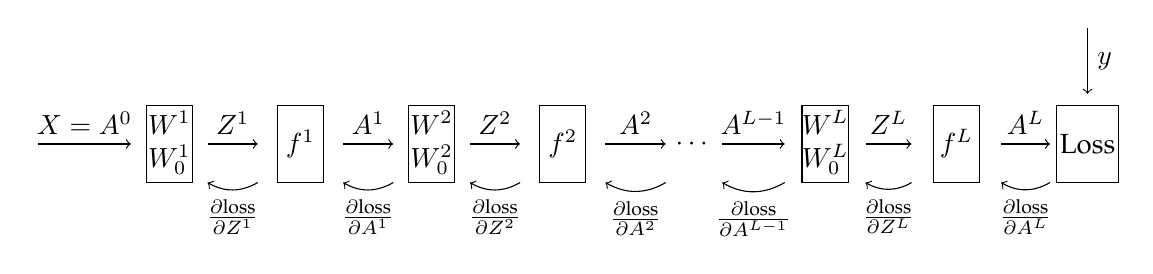
\begin{tikzpicture}[scale=.98]
    \coordinate (x) at (0,0);
    \node[inner sep=0em] (w1) at (1.7,0)
    {\begin{tabular}{c} $W^1$ \\ $W^1_0$\end{tabular}};
    \node[inner sep=1em] (f1) at ($2*(w1)$) {$f^1$};
    \node[inner sep=0em] (w2) at ($3*(w1)$)
    {\begin{tabular}{c} $W^2$ \\ $W^2_0$\end{tabular}};
    \node[inner sep=1em] (f2) at ($4*(w1)$) {$f^2$};
    \node (dots) at ($5*(w1)$) {$\cdots$};
    \node[inner sep=0em] (wL) at ($6*(w1)$)
    {\begin{tabular}{c} $W^L$ \\ $W^L_0$\end{tabular}};
    \node[inner sep=1em] (fL) at ($7*(w1)$) {$f^L$};
    \node (loss) at ($8*(w1)$) {Loss};
    \coordinate (y) at ($8*(w1) + (0,1.5)$);

    \draw[->] (x) -- node[above] {$X = A^0$} (w1);
    \draw[->] (w1) -- node[above] {$Z^1$} (f1);
    \draw[->] (f1) -- node[above] {$A^1$} (w2);
    \draw[->] (w2) -- node[above] {$Z^2$} (f2);
    \draw[->] (f2) -- node[above] {$A^2$} (dots);
    \draw[->] (dots) -- node[above] {$A^{L-1}$} (wL);
    \draw[->] (wL) -- node[above] {$Z^L$} (fL);
    \draw[->] (fL) -- node[above] {$A^L$} (loss);
    \draw[->] (y) -- node[right] {$y$} ($(loss)+(0,.65)$);

    %\draw[->,yshift=0.5cm] (loss.west) to [out=150,in=30] (fL.east);
    \foreach \s/\e/\t in {loss/fL/A^L,
    fL/wL/Z^L,
    wL/dots/A^{L-1},
    dots/f2/A^2,
    f2/w2/Z^2,
    w2/f1/A^1,
    f1/w1/Z^1}{
    \path[->] ($(\s.west) - (0,.5)$) edge[out=210,in=-30] node[below]
      {$\frac{\partial \text{loss}}{\partial \t}$}
    ($(\e.east) - (0,.5)$);
    }
    \foreach \point in {w1, f1, w2, f2, wL, fL}{
        \draw ($(\point) + (-.3,-.5)$) rectangle ($(\point) + (.3,.5)$);
      }
    \draw ($(loss) + (-.4,-.5)$) rectangle ($(loss) + (.4,.5)$);
  \end{tikzpicture}
\end{center}

If we view our neural network as a sequential composition of modules
(in our work so far, it has been an alternation between a linear
transformation with a weight matrix, and a component-wise application
of a non-linear activation function), then we can define a simple API
for a module that will let us compute the forward and backward passes,
as well as do the necessary weight updates for gradient descent.  Each
module has to provide the following ``methods.''  We are already using
letters $a, x, y, z$ with particular meanings, so here we will use $u$
as the vector input to the module and $v$ as the vector output:
\begin{itemize}
  \item forward: $u \rightarrow v$
  \item backward: $u, v, \partial L /
          \partial v \rightarrow \partial L / \partial u$
  \item weight grad: $u, \partial L / \partial v \rightarrow \partial L
          / \partial W$  only needed for modules that have weights $W$
\end{itemize}
In homework we will ask you to implement these modules for neural
network components, and then use them to construct a network and train
it as described in the next section.

% \begin{examplebox}
% What are some conventions for derivatives of matrices and vectors?  It
% will always work to explicitly write all indices and treat everything
% as scalars, but we introduce here some shortcuts that are often faster
% to use and helpful for understanding:
% \begin{itemize}

% \item For $v$ of size $1\times 1$ and $u$ of size $1\times 1$,
%   $\partial v/\partial u$ is the (scalar) partial derivative of $v$
%   w.r.t. $u$.  Example: $\underbrace{\partial L}_{1\times
%     1}/\underbrace{\partial W}_{1\times 1}$ is $1\times 1$

% \item For $v$ of size $1\times 1$ and $u$ of size $b\times 1$,
%   $\partial v/\partial u$ is a vector of size $b\times 1$ with the $j^{\rm th}$ entry $\partial v/\partial u_j$.
%   Example: $\underbrace{\partial L}_{1\times 1}/\underbrace{\partial W_0}_{n\times 1}$ is $n\times 1$

% \item For $v$ of size $c\times 1$ and $u$ of size $b\times 1$,
%   $\partial v/\partial u$ is a vector of size $b\times c$ with the $(j, k)$ entry $\partial v_k/\partial u_j$.
%   Example: $\underbrace{\partial A}_{n\times 1}/\underbrace{\partial Z}_{n\times 1}$ is $n\times n$

% \item For $v$ of size $1\times 1$ and $u$ of size $b\times c$,
%   $\partial v/\partial u$ is a vector of size $b\times c$ with the $(j, k)$ entry $\partial v/\partial u_{j,k}$.
%   Example: $\underbrace{\partial L}_{1\times 1}/\underbrace{\partial W}_{m\times n}$ is $m\times n$

% \end{itemize}
% \end{examplebox}



%\chapter{Making NN's Work}
\section{Training}
Here we go!  Here's how to do stochastic gradient descent training on
a feed-forward neural network.\index{neural network!training}   After this pseudo-code, we motivate
the choice of initialization in lines 2 and 3.  The actual
computation of the gradient values (e.g., $\partial\text{loss}/
  \partial A^L$) is not directly defined in this code, because we want
to make the structure of the computation clear.
\question{What is $\partial Z^l / \partial W^l$? }
\question{Which terms in the code below depend on $f^L$?}

\begin{codebox}
  \Procname{$\proc{SGD-Neural-Net}(\dataTrain, T, L, (m^1, \ldots,
    m^L), (f^1, \ldots, f^L), \text{Loss})$}
    \li     \For $l \gets 1$ \To $L$
    \Do
    \li        $W_{ij}^l \sim \text{Gaussian}(0, 1/m^l)$
    \li        $W_{0j}^l \sim \text{Gaussian}(0, 1)$
    \End
    \li \For $t \gets 1$ \To $T$
    \li   \Do
  $i \gets \text{random sample from } \{1,\ldots,n\}$
    \li     $A^0 \gets \ex{x}{i}$
    \li     \Comment forward pass to compute the output $A^L$
    \li     \For $l \gets 1$ \To $L$
    \li       \Do
  $Z^l \gets W^{l^T}A^{l-1} + W_0^l$
    \li         $A^l \gets f^l(Z^l)$
    \End
    \li     $\text{loss} \gets \text{Loss}(A^L, \ex{y}{i})$
    \li     \For $l \gets L$ \To 1:
    \Do
    \li       \Comment error back-propagation
    \li       $\partial \text{loss}/\partial A^l \gets$ 	%
    %            m x 1
    {\bf if} $l < L$
    {\bf then}
    % dims:          n x 1                    *    m x n
  $\partial Z^{l+1}/\partial A^l \cdot \partial \text{loss}/\partial Z^{l+1} $
    % dims:  m x n                   *     n x 1
    {\bf else}
  $ \partial \text{loss}/\partial A^L$
    \li       $\partial \text{loss}/\partial Z^l \gets \partial
  A^l/\partial Z^l  \cdot \partial
  \text{loss}/\partial A^l$
    \li       \Comment compute gradient with respect to weights
    \li       $\partial \text{loss}/\partial W^l  \gets        A^{l-1}      \cdot    \left( \partial \text{loss}/\partial Z^l  \right)^T $
    %                           m x n              =            m x 1          *        1 x n
    \li       $\partial \text{loss}/\partial W_0^l \gets       \partial \text{loss}/\partial Z^l $
    %                           1 x n              =                  1 x n
    \li       \Comment stochastic gradient descent update
    \li       $W^l = W^l - \eta(t)\cdot \partial \text{loss}/\partial W^l$
    \li       $W^l_0 = W_0^l - \eta(t)\cdot \partial \text{loss}/\partial W_0^l$
  \End
\end{codebox}

Initializing $W$ is important;\index{neural network!initialization of weights}  if you do it badly there is a good
chance the neural network training won't work well.  First, it is
important to initialize the weights to random values.  We want
different parts of the network to tend to ``address'' different
aspects of the problem; if they all start at the same weights, the
symmetry will often keep the values from moving in useful directions.
Second, many of our activation functions have (near) zero slope when
the pre-activation $z$ values have large magnitude, so we generally
want to keep the initial weights small so we will be in a situation
where the gradients are non-zero, so that gradient descent will have
some useful signal about which way to go.

One good general-purpose strategy is to choose each weight at random
from a Gaussian (normal) distribution with mean 0 and standard
deviation $(1/m)$ where $m$ is the number of inputs to the unit.
\question{If the input $x$ to this unit is a vector of 1's, what would
  the expected pre-activation $z$ value be with these initial
  weights?}  We write this choice (where $\sim$ means ``is drawn
randomly from the distribution'') as $W^l_{ij} \sim \text{Gaussian}\left(0,
  \frac{1}{m^l}\right).$ It will often turn out (especially for fancier activations and loss
functions) that computing
$\frac{\partial \text{loss}}{\partial Z^L}$ is easier than computing
$\frac{\partial \text{loss}}{\partial A^L}$ and $\frac{\partial A^L}{\partial Z^L}.$ So, we may instead ask for an implementation of a loss function to provide a backward method that computes $\partial \text{loss}/\partial Z^L$ directly.


\section{Optimizing neural network parameters}
\label{sec-make_nn_work}

Because neural networks are just parametric functions, we can optimize
loss with respect to the parameters using standard gradient-descent
software, but we can take advantage of the structure of the loss
function and the hypothesis class to improve optimization.  As we have
seen, the modular function-composition structure of a neural network
hypothesis makes it easy to organize the computation of the gradient.
As we have also seen earlier, the structure of the loss function as a
sum over terms, one per training data point, allows us to consider
stochastic gradient methods.  In this section we'll consider some
alternative strategies for organizing training, and also for making it
easier to handle the step-size parameter.

\subsection{Batches}
Assume that we have an objective of the form
\[J(W) = \sum_{i = 1}^n \mathcal{L}(h(\ex{x}{i}; W),  \ex{y}{i})\;\;,\]
where $h$ is the function computed by a neural network, and $W$ stands
for all the weight matrices and vectors in the network.

Recall that, when we perform {\em batch} (or the vanilla) gradient descent, we use the update rule
\[W_t = W_{t-1} - \eta\nabla_W J(W_{t-1})\;\;,\]
which is equivalent to
\[W_t = W_{t-1} - \eta\sum_{i=1}^n \nabla_W \mathcal{L}(h(\ex{x}{i}; W_{t-1}),
  \ex{y}{i})\;\;.\]
So, we sum up the gradient of loss at each training point,  with
respect to $W$, and then take a step in the negative direction of
the gradient.

In {\em stochastic} gradient descent, we repeatedly pick a point
$(\ex{x}{i}, \ex{y}{i})$ at random from the data set, and execute a
weight update on that point alone:
\[W_t = W_{t-1} - \eta \nabla_W \mathcal{L}(h(\ex{x}{i}; W_{t-1}),
  \ex{y}{i})\;\;.\]
As long as we pick points uniformly at random from the data set, and
decrease $\eta$ at an appropriate rate, we are guaranteed, with high
probability, to converge to at least a local optimum.

These two methods have offsetting virtues.  The batch method takes
steps in the exact gradient direction but requires a lot of
computation before even a single step can be taken, especially if the
data set is large.  The stochastic method begins moving right away,
and can sometimes make very good progress before looking at even a
substantial fraction of the whole data set, but if there is a lot of
variability in the data, it might require a very small $\eta$ to
effectively average over the individual steps moving in ``competing''
directions.

An effective strategy is to ``average'' between batch and stochastic
gradient descent by using {\em mini-batches}.  For a mini-batch of
size $K$, we select $K$ distinct data points uniformly at random from the data
set and do the update based just on their contributions to the gradient
\[W_t = W_{t-1} - \eta\sum_{i=1}^K \nabla_W \mathcal{L}(h(\ex{x}{i}; W_{t-1}),
  \ex{y}{i})\;\;.\]
Most neural network software packages are set up to do mini-batches.
\question{For what value of $K$ is mini-batch gradient descent
  equivalent to stochastic gradient descent?  To batch gradient
  descent?}

Picking $K$ unique data points at random from a large data-set is
potentially computationally difficult.  An alternative strategy, if
you have an efficient procedure for randomly shuffling the data set
(or randomly shuffling a list of indices into the data set) is to
operate in a loop, roughly as follows:

\begin{codebox}
  \Procname{$\proc{Mini-Batch-SGD}$(NN, data, K)}
  \li     $n = $ length(data)
  \li     \While not done:
  \Do
  \li        $\proc{Random-Shuffle}$(data)
  \li        \For $i \gets 1$ \To $\lceil n/K \rceil$
  \Do
  \li           $\proc{Batch-Gradient-Update}$(NN, data$[(i - 1)K:iK]$)
  \End
  \End
\end{codebox}
See note on the ceiling\footnote{
  In line 4 of the algorithm above, $\lceil \cdot \rceil$ is known
  as the \emph{ceiling} function; it returns the smallest
  integer greater than or equal to its input. E.g., $\lceil 2.5 \rceil = 3$ and $\lceil 3 \rceil = 3$.}
function, for the case when $n/K$ is not an integer.

\subsection{Adaptive step-size}
Picking a value for $\eta$ is difficult and time-consuming.\index{adaptive step size}  If it's
too small, then convergence is slow and if it's too large, then we
risk divergence or slow convergence due to oscillation.  This problem
is even more pronounced in stochastic or mini-batch mode, because we
know we need to decrease the step size for the formal guarantees to
hold.

It's also true that, within a single neural network, we may well want
to have different step sizes.  As our networks become {\em deep} (with
increasing numbers of layers) we can find that magnitude of the
gradient of the loss with respect the weights in the last layer,
$\partial \text{loss} / \partial W_L$, may be substantially
different from the gradient of the loss with respect to the weights in
the first layer $\partial \text{loss} / \partial W_1$.  If you look
carefully at Eq.~\ref{eq:gradz}, you can see that the output
gradient is multiplied by all the weight matrices of the network and
is ``fed back'' through all the derivatives of all the activation
functions.  This can lead to a problem of {\em exploding}  or {\em
    vanishing} gradients\index{exploding (or vanishing) gradients}, in which the back-propagated gradient is much
too big or small to be used in an update rule with the same step size.

So, we can consider having an independent step-size parameter {\em for each
    weight}, and updating it based on a local view of how the gradient
updates have been going.\note{This section is very strongly influenced
by Sebastian Ruder's excellent blog posts on the topic:
{\tt\scriptsize ruder.io/ optimizing-gradient-descent}}
Some common strategies for this include \emph{momentum} (``averaging'' recent gradient updates), \emph{Adadelta} (take larger steps in parts of the space where $J(W)$ is nearly flat), and \emph{Adam} (which combines these two previous ideas). Details of these approaches are described in Appendix~\ref{adaptive-step-size-appendix}. 


\section{Regularization}\index{neural network!regularization}
So far, we have only considered optimizing loss on the training data
as our objective for neural network training.   But, as we have
discussed before, there is a risk of overfitting if we do this.  The
pragmatic fact is that,  in current deep neural networks, which tend to be very
large and to be trained with a large amount of data,  overfitting is
not a huge problem.  This runs counter to our current theoretical
understanding and the study of this question is a hot area of
research.  Nonetheless, there are several strategies for regularizing
a neural network, and they can sometimes be important.

\subsection{Methods related to ridge regression}

One group of strategies can, interestingly, be shown to have similar
effects to each other: early stopping, weight decay, and adding noise
to the training data. \note{Result is due to Bishop, described in his
  textbook and here {\tt\scriptsize doi.org/10.1162/ neco.1995.7.1.108}.}

Early stopping is the easiest to implement and is in fairly common
use.  The idea is to train on your training set, but at every {\em
    epoch} (a pass through the whole training set, or possibly more
frequently), evaluate the loss of the current $W$ on a {\em validation
    set}.  It will generally be the case that the loss on the training
set goes down fairly consistently with each iteration, the loss on the
validation set will initially decrease, but then begin to increase
again.  Once you see that the validation loss is systematically
increasing, you can stop training and return the weights that had the
lowest validation error.

Another common strategy is to simply penalize the norm of all the
weights, as we did in ridge regression.  This  method is known as {\em
    weight decay}\index{neural network!weight decay}, because when we take the gradient of the objective
$$ J(W) = \sum_{i = 1}^{n}\mathcal{L}(\text{NN}(x^{(i)}), y^{(i)}; W)
  + \lambda\|W\|^2 $$
we end up  with an update of the form
\begin{align*}
  W_t & = W_{t-1} -
  \eta\left(\left(\nabla_{W}\mathcal{L}(\text{NN}(x^{(i)}),
  y^{(i)}; W_{t-1})\right) + 2\lambda W_{t-1}\right)                                      \\
      & = W_{t-1}(1 - 2\lambda\eta) - \eta\left(\nabla_{W}\mathcal{L}(\text{NN}(x^{(i)}),
    y^{(i)}; W_{t-1})\right) \;\;.
\end{align*}
This rule has the form of first ``decaying'' $W_{t-1}$ by a factor of
$(1 - 2 \lambda \eta)$ and then taking a gradient step.

Finally, the same effect can be achieved by perturbing the $\ex{x}{i}$
values of the training data by adding a small amount of zero-mean
normally distributed noise before each gradient computation.  It makes
intuitive sense that it would be more difficult for the network to
overfit to particular training data if they are changed slightly on
each training step.

\subsection{Dropout}
Dropout\index{neural network!dropout} is a regularization method that was designed to work with deep
neural networks.  The idea behind it is, rather than perturbing the
data every time we train, we'll perturb the network!  We'll do this by
randomly, on each training step, selecting a set of units in each
layer and prohibiting them from participating.   Thus, all of the
units will have to take a kind of  ``collective'' responsibility for
getting the answer right, and will not be able to rely on any small
subset of the weights to do all the necessary computation.  This tends
also to make the network more robust to data perturbations.

During the training phase, for each training example, for each unit,
randomly with probability $p$ temporarily set $a^{\ell}_j = 0$. There
will be no contribution to the output and no gradient update for the
associated unit.
\question{
  Be sure you understand why, when using {\sc sgd}, setting an
  activation value to 0 will cause that unit's weights not to be updated
  on that iteration.
}

When we are done training and want to use the network to make
predictions, we multiply all weights by $p$ to achieve the same average
activation levels.

Implementing dropout is easy!  In the forward pass during training, we let
$$ a^{\ell} = f(z^{\ell}) * d^{\ell} $$
where $*$ denotes component-wise product and $d^{\ell}$ is a vector of
$0$'s and $1$'s drawn randomly with probability $p$.
The backwards pass depends on $a^{\ell}$, so we do not need to make
any further changes to the algorithm.

It is common to set $p$ to $0.5$, but this is something one might
experiment with to get good results on your problem and data.

% Dropout is no longer in common use, but it is still interesting to
% think about.

\subsection{Batch normalization}

Another strategy that seems to help with regularization and robustness
in training is {\em batch normalization}.  \index{neural network!batch normalization}
\note{For more  details see {\tt\scriptsize arxiv.org/abs/1502.03167}.}
It was originally
developed to address a problem of {\em covariate shift}:  that is, if
you consider the second layer of a two-layer neural network, the
distribution of its input values is changing over time as the first
layer's  weights change.  Learning when the input distribution is
changing is extra difficult:  you have to change your weights to
improve your predictions, but also just to compensate for a change in
your inputs  (imagine, for instance, that the magnitude of the inputs
to your layer is increasing over time---then your weights will have to
decrease, just to keep your predictions the same).

So, when training with mini-batches, the idea is to {\em standardize}
the input values for each mini-batch, just in the way that we did it
in Section~\ref{realFeatures} of Chapter~\ref{chap-features}, subtracting off the mean
and dividing by the standard deviation of each input dimension.  This
means that the scale of the inputs to each layer remains the same, no
matter how the weights in previous layers change.  However, this
somewhat complicates matters, because the computation of the weight
updates will need to take into account that we are performing this
transformation.  In the modular view, batch normalization can be seen
as a module that is applied to $z^l$, interposed after the product
with $W^l$ and before input to $f^l$.\note{We follow here the
  suggestion from the original paper of applying batch normalization
  before the activation function.  Since then it has been shown that,
  in some cases, applying it after works a bit better. But there
  aren't any definite findings on which works better and when.}

Although batch-norm was originally justified based on the problem of
covariate shift, it's not clear that that is actually why it seems to
improve performance.
Batch normalization can also end up having a regularizing effect for similar
reasons that adding noise and dropout do:  each mini-batch of data
ends up being mildly perturbed, which prevents the network from
exploiting very particular values of the data points.
For those interested, the equations for batch normalization, including a derivation of the forward pass and backward pass, are described in Appendix~\ref{batch-norm-appendix}.


%%% Local Variables:
%%% mode: latex
%%% TeX-master: "top"
%%% End:


%%%%%%%%%%%%%%%%%%%%%%%%%%%%%%%%%%%%%%%%%%%%%%%%%%%%%%%%%%%%%%%%%%%%%%%%%%%%%

%%% Local Variables:
%%% mode: latex
%%% TeX-master: "top"
%%% End:

\chapter{Convolutional Neural Networks}
\label{chap-cnn}

So far, we have studied what are called {\em fully connected} neural
networks, in which all of the units at one layer are connected to all
of the units in the next layer. This is a good arrangement when we
don't know anything about what kind of mapping from inputs to outputs
we will be asking the network to learn to approximate.  But if we {\em
    do} know something about our problem, it is better to build it into
the structure of our neural network.  Doing so can save
computation time and significantly diminish the amount of training
data required to arrive at a solution that generalizes robustly.

One very important application domain of neural networks, where the
methods have achieved an enormous amount of success in recent years,
is signal processing.  Signals might be spatial (in two-dimensional
camera images or three-dimensional depth or CAT scans) or temporal
(speech or music).   If we know that we are addressing a
signal-processing problem, we can take advantage of {\em invariant}
properties of that problem.  In this chapter, we will focus on
two-dimensional spatial problems (images) but use one-dimensional ones
as a simple example.  In a later chapter, we will address temporal problems.

Imagine that you are given the problem of designing and training a
neural network that takes an image as input, and outputs a
classification, which is positive if the image contains a cat and
negative if it does not.  An image is described as a two-dimensional
array of {\em pixels}\note{A {\em pixel} is a ``picture element.''},
each of which may be represented by three integer values, encoding
intensity levels in red, green, and blue color channels.

There are two important pieces of prior structural knowledge
we can bring to bear on this problem:
\begin{itemize}
  \item{\bf Spatial locality:} \index{spatial locality} The set of pixels we will have to take
        into consideration to find a cat will be near one another in the
        image. \note{So, for example, we won't have to consider some combination
          of pixels in the four corners of the image, in order to see if they encode
          cat-ness.}

  \item{\bf Translation invariance:} \index{translation invariance} The pattern of pixels that
        characterizes a cat is the same no matter where in the image the cat
        occurs. \note{Cats don't look different if they're on the left or
          the right side of the image.}
\end{itemize}

We will design neural network structures that take advantage of these
properties.

\pagebreak
\section{Filters}
We begin by discussing {\em image filters}\note{Unfortunately in
  AI/ML/CS/Math, the word ``filter'' gets used in many ways: in
  addition to the one we describe here, it can describe a temporal
  process (in fact, our moving averages are a kind of filter) and even
  a somewhat esoteric algebraic structure.}.  An image filter is a
function that takes in a local spatial neighborhood of pixel values
and detects the presence of some pattern in that data.\index{filter}

Let's consider a very simple case to start, in which we have a
1-dimensional binary ``image'' and a filter $F$ of size two.  The
filter is a vector of two numbers, which we will move along the image,
taking the dot product between the filter values and the image values
at each step, and aggregating the outputs to produce a new image.

Let $X$ be the original image, of size $d$; then pixel $i$ of the the
output image is specified by
\[Y_i = F \cdot  (X_{i-1}, X_i)\;\;.\]
To ensure that the output
image is also of dimension $d$, we will generally ``pad'' the input
image with 0 values if we need to access pixels that are beyond the
bounds of the input image.  This process of applying the filter to the
image to create a new image is called ``convolution.''\index{convolution}\index{convolutional neural network}\note{And
  filters are also sometimes called {\em convolutional kernels}.}

If you are already familiar with what a convolution is, you might
notice that this definition corresponds to what is often called a
correlation and not to a convolution. Indeed, correlation and
convolution refer to different operations in signal
processing. However, in the neural networks literature, most libraries
implement the correlation (as described in this chapter) but call it
convolution. The distinction is not significant; in principle, if
convolution is required to solve the problem, the network could learn
the necessary weights.
For a discussion of the difference between convolution
and correlation and the conventions used in the literature you can
read Section~9.1 in this excellent book: {\tt
https://www.deeplearningbook.org}.

Here is a concrete example.  Let the filter $F_1 = (-1, +1)$.  Then
given the image in the first line below,  we can convolve it with filter $F_1$ to
obtain the second image.  You can think of this filter as a detector
for ``left edges'' in the original image---to see this, look at the
places where there is a $1$ in the output image, and see what pattern
exists at that position in the input image.  Another interesting filter
is $F_2 =  (-1, +1, -1)$.  The third image (the last line below)
shows the result of convolving the first image with $F_2$,
where we see that the output pixel $i$ corresponds to when the center
of $F_2$ is aligned at input pixel $i$.
\question{Convince yourself that filter $F_2$ can be understood as a
  detector for isolated positive pixels in the binary image.}
\medskip

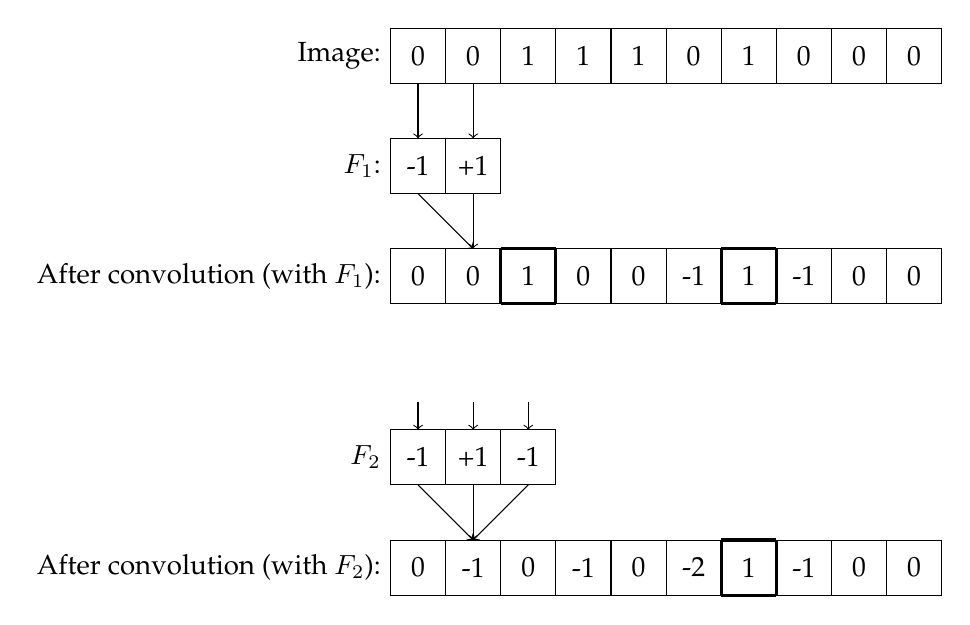
\begin{tikzpicture}[x=0.7cm, y=0.7cm, step=0.7cm]
  %LPK: to make this work with includeonly, due to a bug in tex, we
  %have to define this counter in the preamble
  %\newcounter{col}
  \begin{scope}
    \draw (0, 0) grid (10, 1);
    \setcounter{col}{1}
    \foreach \p in {0,0,1,1,1,0,1,0,0,0} {
        \edef\x{\value{col} - 0.5}
        \node[anchor=center] at (\x, 0.5) {\p};
        \stepcounter{col}
      }
    \node[left] at (0,0.5) {Image:};
    \draw (0, -2) grid (2, -1);
    \node[left] at (0, -1.5) {$F_1$:};
    \node[anchor=center] (f11) at (0.5, -1.5) {-1};
    \node[anchor=center] (f12) at (1.5, -1.5) {+1};

    \coordinate (x1) at (0.5, 0);
    \coordinate (x2) at (1.5, 0);
    \draw[->] (x1) -- ++(0,-1);
    \draw[->] (x2) -- ++(0,-1);
    \draw[->] (x1)++(0,-2) -- ++(1,-1);
    \draw[->] (x2)++(0,-2) -- ++(0,-1);
  \end{scope}
  \begin{scope}[yshift=-2.8cm]
    \draw (0, 0) grid (10, 1);
    \setcounter{col}{1}
    \foreach \p in {0,0,1,0,0,-1,1,-1,0,0} {
        \edef\x{\value{col} - 0.5}
        \node[anchor=center] at (\x, 0.5) {\p};
        \stepcounter{col}
      }
    \node[left] at (0,0.5) {After convolution (with $F_1$):};
    \draw[very thick] (2, 0) grid (3, 1);
    \draw[very thick] (6, 0) grid (7, 1);
  \end{scope}
  \begin{scope}[yshift=-6.5cm]
    \draw (0, 0) grid (10, 1);
    \setcounter{col}{1}
    \foreach \p in {0,-1,0,-1,0,-2,1,-1,0,0} {
        \edef\x{\value{col} - 0.5}
        \node[anchor=center] at (\x, 0.5) {\p};
        \stepcounter{col}
      }
    \node[left] at (0,0.5) {After convolution (with $F_2$):};
    \draw (0, 2) grid (3, 3);
    \node[left] at (0, 2.5) {$F_2$};
    \draw[very thick] (6, 0) grid (7, 1);
    \node[anchor=center] at (0.5, 2.5) {-1};
    \node[anchor=center] at (1.5, 2.5) {+1};
    \node[anchor=center] at (2.5, 2.5) {-1};

    \coordinate (x1) at (0.5, 4);
    \coordinate (x2) at (1.5, 4);
    \coordinate (x3) at (2.5, 4);
    \draw[->] (x1)++(0,-0.5) -- ++(0,-0.5);
    \draw[->] (x2)++(0,-0.5) -- ++(0,-0.5);
    \draw[->] (x3)++(0,-0.5) -- ++(0,-0.5);
    \draw[->] (x1)++(0,-2) -- ++(1,-1);
    \draw[->] (x2)++(0,-2) -- ++(0,-1);
    \draw[->] (x3)++(0,-2) -- ++(-1,-1);
  \end{scope}
\end{tikzpicture}

Two-dimensional versions of filters like these are thought to be found
in the visual cortex of all mammalian brains. Similar patterns arise from
statistical analysis of natural images.  Computer vision people used
to spend a lot of time hand-designing {\em filter banks}.  A filter
bank is a set of sets of filters, arranged as shown in the diagram
below.

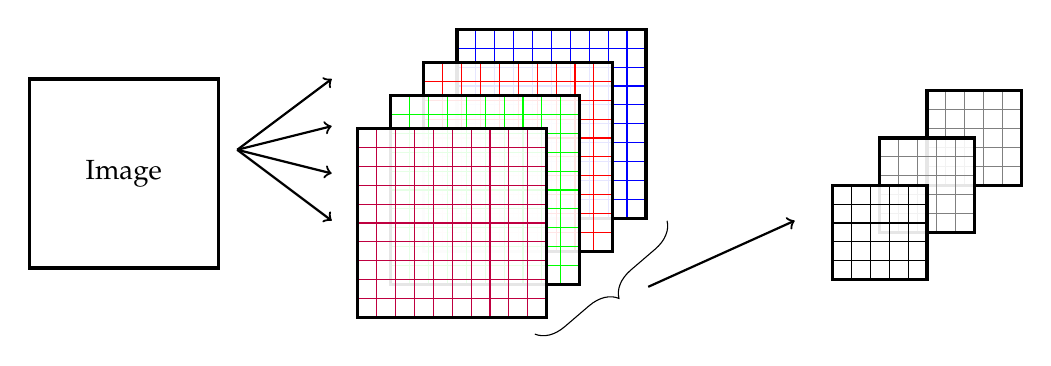
\begin{tikzpicture}[scale=0.6]
  \begin{scope}
    \draw[black,very thick] (0,0) rectangle (4,4);%marking borders
    \node[anchor=center] at (2,2) {Image};
  \end{scope}

  \coordinate (x) at (4.4, 2.5);
  \foreach \yoff in {-1.5,-.5,.5,1.5} {
      \draw[->,thick] (x) -- ++(2,\yoff);
    }

  \begin{scope}[xshift=8cm]
    \foreach \shift/\c in {10.5mm/blue,3.5mm/red,-3.5mm/green,-10.5mm/purple} {
        \begin{scope}[xshift=\shift, yshift=\shift]
          \fill[white,fill opacity=0.9] (0,0) rectangle (4,4);
          \draw[step=4mm, color=\c] (0,0) grid (4,4); %defining grids
          \draw[black,very thick] (0,0) rectangle (4,4);%marking borders
        \end{scope}
      }
    \draw [decorate,decoration={brace,mirror,amplitude=10pt}]
    (2.7,-1.4) -- node (layers) {} (5.5,1);
    \coordinate (r) at (8.2, 1);
    \draw[->,thick] ($(layers)+(1,-0.2)$) -- (r);
  \end{scope}

  \begin{scope}[xshift=18cm,yshift=0.75cm]
    \foreach \shift/\c in {10mm/gray,-0mm/gray,-10mm/black} {
        \begin{scope}[xshift=\shift, yshift=\shift]
          \fill[white,fill opacity=0.9] (0,0) rectangle (2,2);
          \draw[step=4mm, color=\c] (0,0) grid (2,2); %defining grids
          \draw[black,very thick] (0,0) rectangle (2,2);%marking borders
        \end{scope}
      }
  \end{scope}
\end{tikzpicture}

All of the filters in the first group are applied to the original
image;  if there are $k$ such filters, then the result is $k$ new
images,   which are called {\em channels}\index{filter!channels}.  Now imagine stacking all
these new images up so that we have a cube of data, indexed by the
original row and column indices  of the image,  as well as by the
channel.  The next set of filters in the filter bank will generally be
  {\em three-dimensional}:  each one will be applied to a sub-range of the
row and column indices of the image and to all of the channels.

These 3D chunks of data are called {\em tensors}\index{tensor}.
\note{There are now many useful neural-network software packages, such
  as {\em TensorFlow} and {\em PyTorch} that make operations on tensors easy.}
The algebra of tensors is fun, and a lot like matrix algebra,  but we
won't go into it in any detail.

Here is a more complex example of two-dimensional filtering.  We have
two $3 \times 3$ filters in the first layer, $f_1$  and $f_2$.  You
can think of each one as ``looking'' for three pixels in a row, $f_1$
vertically and $f_2$ horizontally.  Assuming our input  image is $n
  \times n$, then the result of filtering with these two filters is an $n
  \times n \times 2$ tensor.  Now we apply a tensor filter (hard to
draw!) that ``looks for'' a combination of two horizontal and two vertical
bars  (now represented by individual pixels in the two channels),
resulting in a single final $n \times  n$ image.
\note{When we have a color image as input,  we treat it as having three
  channels, and hence as an $n \times  n \times 3$ tensor.}

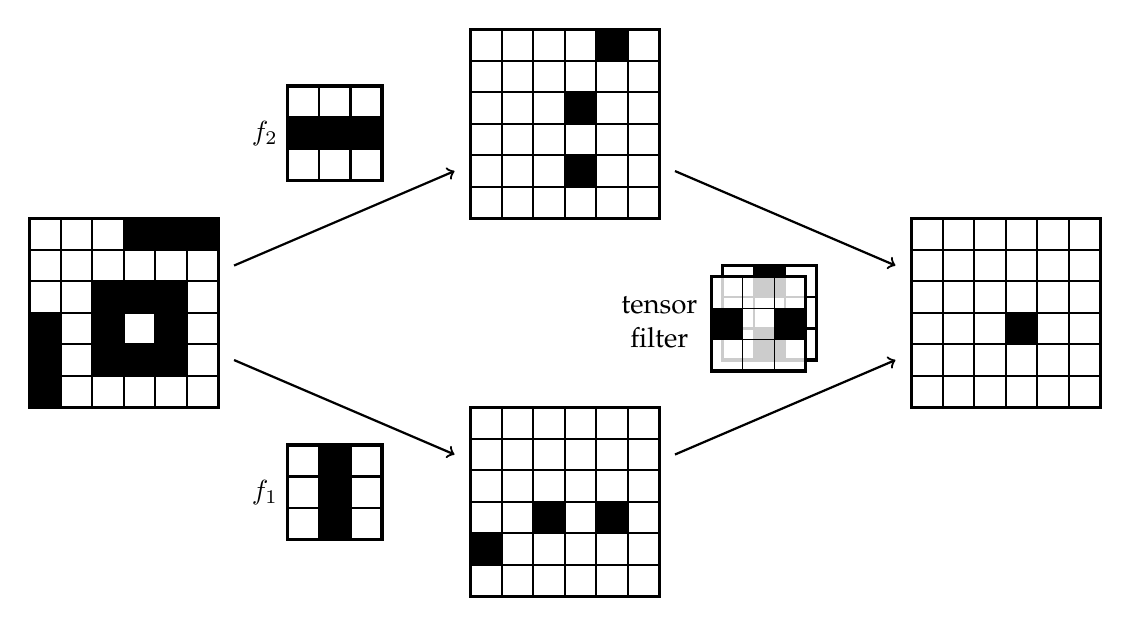
\begin{tikzpicture}[scale=0.4]
  \begin{scope}
    \foreach \x/\y in {0/0,0/1,0/2,2/1,2/2,2/3,3/1,3/3,4/1,4/2,4/3,
        3/5,4/5,5/5} {
        \fill[black] ($(\x,\y)$)
        rectangle ($(\x,\y)+(1,1)$);
      }
    \draw[black,thick] (0,0) grid (6,6);
    \draw[black,very thick] (0,0) rectangle (6,6);
    \draw[->,thick] (6.5,4.5) -- (13.5, 7.5);
    \draw[->,thick] (6.5,1.5) -- (13.5, -1.5);
    \begin{scope}[xshift=8.2cm,yshift=7.2cm]
      \foreach \x/\y in {0/1,1/1,2/1} {
          \fill[black] ($(\x,\y)$)
          rectangle ($(\x,\y)+(1,1)$);
        }
      \draw[black,thick] (0,0) grid (3,3);
      \draw[black,very thick] (0,0) rectangle (3,3);
      \node[left] at (0,1.5) {$f_2$};
    \end{scope}
    \begin{scope}[xshift=8.2cm,yshift=-4.2cm]
      \foreach \x/\y in {1/0,1/1,1/2} {
          \fill[black] ($(\x,\y)$)
          rectangle ($(\x,\y)+(1,1)$);
        }
      \draw[black,thick] (0,0) grid (3,3);
      \draw[black,very thick] (0,0) rectangle (3,3);
      \node[left] at (0,1.5) {$f_1$};
    \end{scope}
  \end{scope}
  \begin{scope}[xshift=14cm, yshift=6cm]
    \foreach \x/\y in {3/1,3/3,4/5} {
        \fill[black] ($(\x,\y)$)
        rectangle ($(\x,\y)+(1,1)$);
      }
    \draw[black,thick] (0,0) grid (6,6);
    \draw[black,very thick] (0,0) rectangle (6,6);
    \draw[->,thick] (6.5,1.5) -- (13.5, -1.5);
  \end{scope}
  \begin{scope}[xshift=14cm, yshift=-6cm]
    \foreach \x/\y in {0/1,2/2,4/2} {
        \fill[black] ($(\x,\y)$)
        rectangle ($(\x,\y)+(1,1)$);
      }
    \draw[black,thick] (0,0) grid (6,6);
    \draw[black,very thick] (0,0) rectangle (6,6);
    \draw[->,thick] (6.5,4.5) -- (13.5, 7.5);
  \end{scope}
  \begin{scope}[xshift=22cm,yshift=1.5cm]
    \foreach \x/\y in {1/0,1/2} {
        \fill[black] ($(\x,\y)$)
        rectangle ($(\x,\y)+(1,1)$);
      }
    \draw[black,thick] (0,0) grid (3,3);
    \draw[black,very thick] (0,0) rectangle (3,3);

    \begin{scope}[xshift=-0.35cm,yshift=-0.35cm]
      \fill[white,fill opacity=0.8] (0,0) rectangle (3,3);
      \foreach \x/\y in {0/1,2/1} {
          \fill[black] ($(\x,\y)$)
          rectangle ($(\x,\y)+(1,1)$);
        }
      \draw[black] (0,0) grid (3,3);
      \draw[black,very thick] (0,0) rectangle (3,3);
      \node[left] at (0.4,1.5) {\begin{tabular}{c}tensor \\
          filter\end{tabular}};
    \end{scope}
  \end{scope}
  \begin{scope}[xshift=28cm]
    \fill[black] (3,2) rectangle (4,3);
    \draw[black,thick] (0,0) grid (6,6);
    \draw[black,very thick] (0,0) rectangle (6,6);
  \end{scope}
\end{tikzpicture}

We are going to design neural networks that have this structure.  Each
``bank'' of the filter bank will correspond to a neural-network
layer.  The numbers in the individual filters will be the ``weights''
(plus a single additive bias or offset value for each filter)
of the network, that we will train using gradient descent.  What
makes this interesting and powerful (and somewhat confusing at first)
is that the same weights are used many many times in the computation
of each layer.  This {\em weight sharing}\index{weight sharing} means that we can express a
transformation on a large image with relatively few parameters; it
also means we'll have to take care in figuring out exactly how to
train it!

We will define a filter layer $l$ formally with:
\note{For simplicity, we are assuming that  all images and filters are
  square (having the same number of  rows and columns).  That is in no
  way  necessary, but is usually fine and definitely simplifies our notation.}
\begin{itemize}
  \item {\em number} of filters $m^l$;
  \item {\em size} of one filter is $k^l \times k^l \times m^{l-1}$ plus $1$ bias
        value (for this one filter);
  \item {\em stride} $s^l$ is the spacing at which we apply the filter
        to the image;  in all of our examples so far, we have used a stride
        of 1, but if we were to ``skip'' and apply the filter only at
        odd-numbered indices of the image, then it would have a stride of
        two (and produce a resulting image of half the size);
  \item {\em input tensor size} $n^{l-1} \times n^{l-1} \times m^{l-1}$
  \item {\em padding}: $p^l$ is how many extra pixels -- typically with value 0 --
        we add around the edges of the input. For an input of size  $n^{l-1} \times n^{l-1} \times m^{l-1}$,
        our new effective input size with padding becomes $(n^{l-1} + 2 \cdot p^l) \times (n^{l-1} + 2 \cdot p^l) \times m^{l-1}$.
\end{itemize}
This layer will produce an output tensor of size $n^l \times n^l \times
  m^l$, where $n^l = \lceil (n^{l-1} + 2 \cdot p^l - (k^l - 1)) / s^l \rceil$.\footnote{
  Recall that $\lceil \cdot \rceil$ is the \emph{ceiling} function; it returns the smallest
  integer greater than or equal to its input. E.g., $\lceil 2.5 \rceil = 3$ and $\lceil 3 \rceil = 3$.}
The weights are the values defining the filter: there will be $m^l$
different $k^l \times k^l \times m^{l-1}$ tensors of weight values; plus
each filter may have a bias term, which means there is one more weight value per
filter.
A filter with a bias operates just like the filter examples above, except we
add the bias to the output. For instance, if we incorporated a bias term of 0.5 into
the filter $F_2$ above, the output would be $(-0.5,0.5,-0.5,0.5, -1.5, 1.5,-0.5,0.5)$
instead of $(-1,0,-1,0,-2,1,-1,0)$.

This may seem complicated, but we get a rich class of mappings that
exploit image structure and have many fewer weights than a fully
connected layer would.
\question{
  How many weights are in a convolutional layer specified as above?}
\question{
  If we used a fully-connected layer with the same size inputs and
  outputs, how many weights would it have?}

\section{Max pooling}\index{max pooling}
It is typical \note{Both in engineering and in nature} to structure
filter banks into a {\em pyramid}, in which the image sizes get
smaller in successive layers of processing.  The idea is  that we find
local patterns, like bits of edges in the early layers, and then look
for patterns  in those patterns, etc.   This means that, effectively,
we are looking for patterns in larger pieces of the image as we apply
successive filters.  Having a stride greater than one makes the images
smaller, but does not necessarily aggregate information over that
spatial range.

Another common layer type, which accomplishes this aggregation, is
  {\em max pooling}.
A max pooling layer operates like a filter, but has no weights. {\em
    You can think of it as purely functional, like a ReLU in a fully connected network.}  It has a filter size\index{filter!filter size}, as in a filter
layer, but simply returns the maximum value in its field.
\note{We sometimes use the term {\em receptive field} or just {\em
      field} to mean the area of an input image that a filter is being
  applied to.}
Usually, we
apply max pooling with the following traits:
\begin{itemize}
  \item $\text{stride} > 1$,  so that the resulting image is smaller
        than the input image; and
  \item $k \geq \text{stride}$, so that the whole image is covered.
\end{itemize}
As a result of applying a max pooling layer, we don't keep track of
the precise location of a pattern. This helps our filters to learn to
recognize patterns independent of their location.

Consider a max pooling layer where both the strides and $k$ are set to be 2. This would
map a $64 \times 64 \times 3$ image to a $32 \times 32 \times 3$
image. Note that max pooling layers do not have additional bias or
offset values.
\question{Maximilian Poole thinks it would be a good idea to add two
  max pooling layers of size $k$, one right after the other, to their
  network.  What single layer would be equivalent?}

One potential concern about max-pooling layers is that they
actually don't completely preserve translation invariance. If you do
max-pooling with a stride other than 1 (or just pool over the whole
image size), then shifting the pattern you are hoping to detect within
the image by a small amount can change the output of the max-pooling
layer substantially, just because there are discontinuities induced by
the way the max-pooling window matches up with its input image.
Here is an interesting paper \note{https://arxiv.org/\\pdf/1904.11486.pdf}
that illustrates this phenomenon clearly
and suggests that one should first do max-pooling with a stride of 1,
then do ``downsampling'' by averaging over a window of outputs.

\section{Typical architecture}
Here is the form of a typical convolutional network:
\begin{figure}[H]
  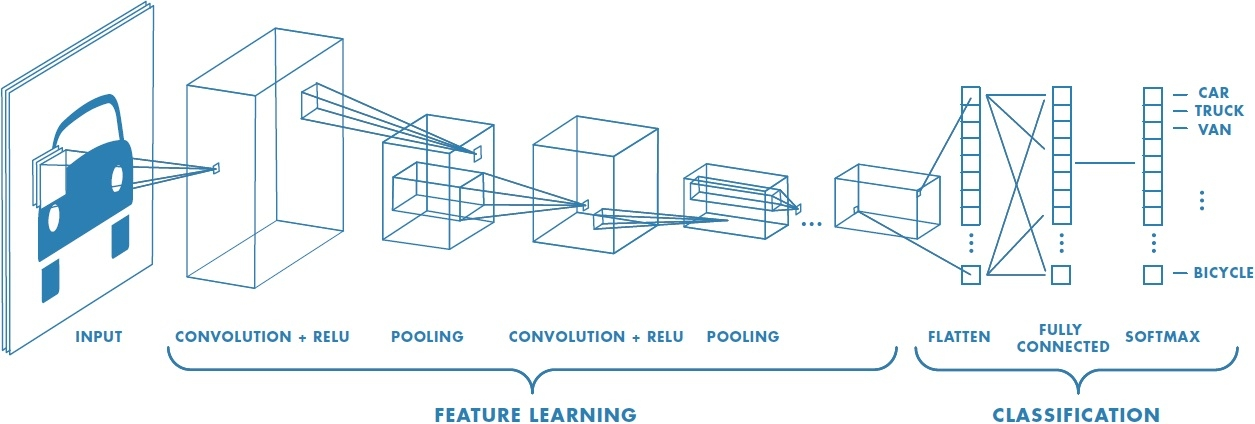
\includegraphics[width=\textwidth]{figures/cnn}
  \caption*{The ``depth'' dimension in the layers shown as cuboids
    corresponds to the number of channels in the output tensor.
    (Figure source: https://www.mathworks.com/solutions/deep-learning/convolutional-neural-network.html)}
\end{figure}

At the end of each filter layer, we typically apply a ReLU activation function. There may be multiple filter plus ReLU layers. Then we have a max pooling layer. Then we have some more filter + ReLU layers. Then we have max pooling again. Once the output is down to
a relatively small size, there is typically a last fully-connected
layer, leading into an activation function such as softmax that
produces the final output. The exact design of these structures is
an art---there is not currently any clear theoretical  (or even
systematic empirical) understanding of how these various design
choices affect overall performance of the network.

The critical point for us is that this is all just a big neural
network, which takes an input and computes an output.  The mapping is
a differentiable function
\note{Well, techinically the derivative does not exist at every point, both because of the ReLU
  and the max pooling operations, but we ignore that fact.}
of the weights, which means we can adjust the weights to decrease the
loss by performing gradient descent, and we can compute the relevant
gradients using back-propagation!

\section{Backpropagation in a simple CNN}

\index{convolutional neural network!backpropagation}
Let's work through a {\em very} simple example of how back-propagation
can work on a convolutional network.   The architecture is shown
below.   Assume we have a one-dimensional single-channel image $X$ of
size $n \times 1 \times 1$, and a single filter $W^1$ of size $k \times 1 \times 1$
(where we omit the filter bias)
for the first convolutional operation denoted ``conv'' in the figure below.
Then we pass the intermediate result $Z^1$
through a ReLU layer to obtain the activation $A^1$,
and finally through a
fully-connected layer with weights $W^2$, denoted ``fc'' below, with no additional
activation function, resulting in the output $A^2$.

\begin{center}
  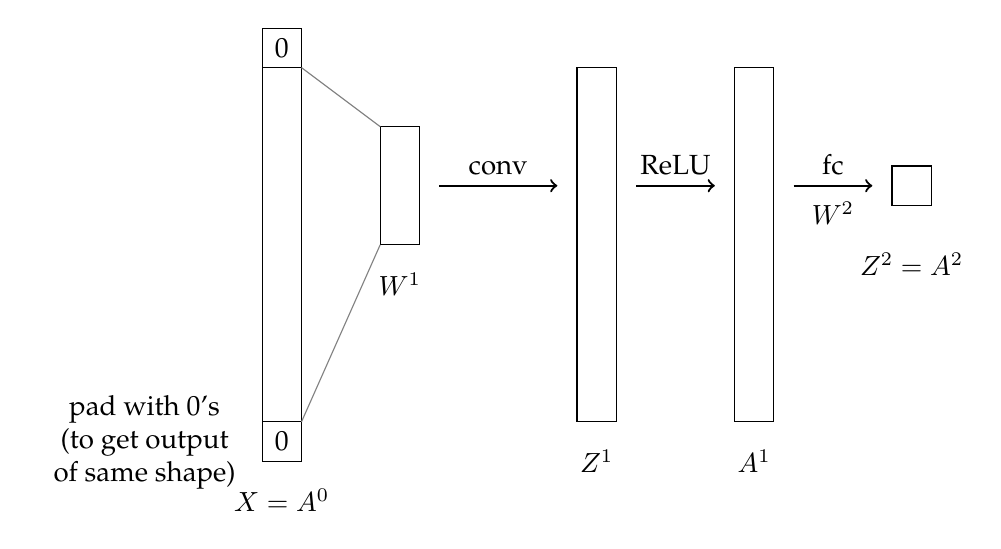
\begin{tikzpicture}[scale=0.5]
    \draw (0,0) rectangle (1,9);
    \node at (.5, -2) {$X = A^0$};
    \draw (0,-1) rectangle (1,0);
    \draw (0,9) rectangle (1,10);
    \node[anchor=center] at (0.5,-.5) {0};
    \node[anchor=center] at (0.5,9.5) {0};
    \node[left] at (0,-0.5) {\begin{tabular}{c}
        pad with 0's \\ (to get output\\ of same shape)\end{tabular}};

    \draw (3,4.5) rectangle (4,7.5);
    \draw[gray] (1,9) -- (3,7.5);
    \draw[gray] (1,0) -- (3,4.5);
    \node at (3.5,3.5) {$W^1$};

    \draw (8,0) rectangle (9,9);
    \node at (8.5,-1) {$Z^1$};

    \draw (12,0) rectangle (13,9);
    \node at (12.5,-1) {$A^1$};

    \draw (16,5.5) rectangle (17,6.5);
    \node at (16.5, 4.0) {$Z^2=A^2$};

    \node at (14.5,5.3) {$W^2$};

    \draw[->,thick] (4.5,6) -- node[above] {conv} (7.5,6);
    \draw[->,thick] (9.5,6) -- node[above] {ReLU} (11.5,6);
    \draw[->,thick] (13.5,6) -- node[above] {fc} (15.5,6);
  \end{tikzpicture}
\end{center}

For simplicity assume $k$ is odd, let the input image $X = A^0$, and
assume we are using squared loss.   Then we can describe the forward
pass as follows:
\begin{align*}
  Z_i^1                        & = {W^1}^TA^0_{[i-\lfloor k/2 \rfloor
  : i + \lfloor k/2 \rfloor]}                                         \\
  A^1                          & = ReLU(Z^1)                          \\
  A^2                          & = Z^2 = {W^2}^T A^1                  \\
  \mathcal{L}_{square}(A^2, y) & = (A^2-y)^2
\end{align*}

\question{Assuming a stride of $1,$ for a filter of size $k$, how much padding do we need to add to the top and bottom of the image? We see one zero at the top and bottom in the figure just above; what filter size is implicitly being shown in the figure? (Recall the padding is for the sake of getting an output the same size as the input.)}

\subsection{Weight update}
How do we update the weights in filter $W^1$?
\[\frac{\partial \text{loss}}{\partial W^1}
  = \frac{\partial Z^1}{\partial W^1}
  \frac{\partial A^1}{\partial Z^1}
  \frac{\partial \text{loss}}{\partial A^1}\]
\begin{itemize}
  \item $\partial Z^1/\partial W^1$ is the $k \times n$
        matrix such that $\partial Z_i^1/\partial W_j^1 =
          X_{i-\lfloor k/2 \rfloor+j-1}$.  So, for example, if $i = 10$,
        which corresponds to column 10 in this matrix, which illustrates
        the dependence of pixel 10 of the output image on the weights, and
        if  $k = 5$, then the
        elements in column 10 will  be $X_8, X_9, X_{10}, X_{11},
          X_{12}$.
  \item $\partial A^1/\partial Z^1$ is the $n \times n$
        diagonal matrix such that
        \begin{eqnarray*}\partial A_i^1/\partial Z_i^1=
          \begin{cases}
            1 & \text{if $Z_i^1 > 0$} \\
            0 & \text{otherwise}
          \end{cases}
        \end{eqnarray*}
  \item $\partial \text{loss}/{\partial A^1}
          = (\partial \text{loss} / {\partial A^2})
          (\partial A^2 / {\partial A^1})
          = 2(A^2 - y)W^2$, an $n \times 1$ vector
\end{itemize}
Multiplying these components yields the desired gradient, of shape
$k \times 1$.

\subsection{Max pooling}
One last point is how to handle back-propagation through a max-pooling
operation.  Let's study this via a simple example.  Imagine
\[y = \max(a_1, a_2)\;\;,\]
where $a_1$ and $a_2$ are each computed by some network.
Consider doing back-propagation through the maximum. First consider the case where $a_1 > a_2$. Then the error %$\delta$ 
value at $y$ is propagated back entirely to the network computing the value  $a_1$. The weights in the network computing  $a_1$ will ultimately be adjusted, and the network computing  $a_2$ will be untouched.
\question{What is $\nabla_{(x, y)} \max(x, y)$ ? }


%%% Local Variables:
%%% mode: latex
%%% TeX-master: "top"
%%% End:

\chapter{Transformers}
\label{chap-transformers}

Transformers are a very recent family of architectures that have revolutionized fields like natural language processing (NLP), image processing, and multi-modal generative AI.


Transformers were originally introduced in the field of NLP in 2017, as an approach to process and understand human language. Human language is inherently sequential in nature (e.g., characters form words, words form sentences, and sentences form paragraphs and documents). Prior to the advent of the transformers architecture, recurrent neural networks (RNNs) briefly dominated the field for their ability to process sequential information (RNNs are described in Appendix \ref{chap-rnn} for reference). However, RNNs, like many other architectures, processed sequential information in an iterative/sequential fashion, whereby each item of a sequence was individually processed one after another. Transformers offer many advantages over RNNs, including their ability to process all items in a sequence in a \textit{parallel} fashion (as do CNNs).

% Transformers were originally introduced in the field of NLP, where they were used to model sequences of characters and words. There, transformers demonstrated significant improvements in the ability to model and understand complex and long data sequences. As a result, many texts present transformers as an alternative to the so-called recurrent neural nets (RNNs) for sequence modeling (RNNs are described in Chapter \ref{chap-rnn} for reference). In terms of the mechanics, however, transformer layers are \textit{parallel} processing machines, like convolutional layers, rather than sequential machines as RNNs are. This parallel nature is one of the main reasons for the effectiveness of transformers; and motivates our presentation below\footnote{The presentation of this chapter largely follows the book {\em Foundations of Computer Vision}, Transformer's Chapter, written by Philip Isola.}.

% Convolutional neural networks model patterns in space, and recurrent neural networks model patterns in time.  In both cases, the models look for locality, and by doing so the number of model parameters $\theta$ is kept relatively small, and can be made independent of the size $n$ of the dataset.  This makes CNNs and RNNs efficient to describe, and helps make them trainable.  However, these models struggle with patterns that are extended in space or time; for example, how do we efficiently account for the influence of words that appear early on in a sentence on much later parts?  In these models, when addressing such problems using long-range patterns, the gradients calculated during backpropagation often are too small to stably update the value of a weight.

Like CNNs, transformers factorize the signal processing problem into stages that involve independent and identically processed chunks. However, they also include layers that mix information across the chunks, called {\em attention layers,} so that the full pipeline can model dependencies between the chunks.

In this chapter, we describe transformers from the bottom up. We start with the idea of embeddings and tokens (Section~\ref{sec-embeddings}). We then describe the attention mechanism (Section~\ref{sec-qkv}). And finally we then assemble all these ideas together to arrive at the full transformer architecture in Section~\ref{sec-transformers}.

%%%%%%%%%%%%%%%%%%%%%%%%%%%%%%%%%%%%%%%%%%%%%%%%%%%%%%%%%%%%%%%%%%%%%%%%%%%%%
\section{Vector embeddings and tokens}
\label{sec-embeddings}

% - word2vec
%   - vector diagram: sweet savory sugar salt
%     paris – france + poland = warsaw
%   - vector addition
%   - cosine distance
%   - conditional PDF
%   - how to train for embeddings
%   - tokens (word fragments, sentences, subimages)

% concept of semantic embedding
Before we can understand the attention mechanism in detail, we need to first introduce a new data structure and a new way of thinking about neural processing for language.

% CHRIS' VERSION
The field of NLP aims to represent words with vectors (aka {\em word embeddings}) such that they capture semantic meaning. More precisely, the degree to which any two words are related in the `real-world' to us humans should be reflected by their corresponding vectors (in terms of their numeric values). So, words such as `dog' and `cat' should be represented by vectors that are more similar to one another than, say, `cat' and `table' are. Nowadays, it's also typical for every individual occurrence of a word to have its own distinct representation/vector. So, a story about a dog may mention the word `dog' a dozen times, with each vector being slightly different based on its context in the sentence and story at large.

To measure how similar any two word embeddings are (in terms of their numeric values) it is common to use {\em cosine similarity} as the metric:

% ORIG VERSION (i'd remove this)
%Consider the challenge of understanding human language.  Words that appear to be very different may have quite similar semantics to a listener, depending on the context in which they are used.  For example, ``sweet'' is to ``sugar'' as ``savory'' is to ``salt'', and it is desirable to be able to capture such semantic relationships by mapping words to numerical vectors, e.g., representing word $w$ with a $d$-dimensional vector $v_w$.  Such multidimensional vectors are typically termed as ``tokens'' in the transformers literature.

% \note{In language modeling, a token might represent a word, so that a sequence of tokens is a sentence. In computer vision, a token may correspond to an image patch, so that an array of tokens represents an image}. 

% CT: I'd remove this, too
%The tokenization of words (or other kinds of raw data) help capture the fact that some words statistically occur closer to other words in written text.  For example, ``quantum'' likely appears more often in the vicinity of ``physics'' than near ``weather,'' whereas ``rain'' and ``weather'' are more likely to occur in proximity to each other.

% older draft
% This is the goal, but not the mechanism. E.g., word2vec uses a skipgram model (which you discuss below). The intuition that is difficult for people (me, for instance) is why the thetas of that model make a good embedding. It would be great if you could motivate that. What's confusing is that these embeddings are not constructed by knowing semantic similarities, only by knowing co-occurrence patterns among tokens.


% ORIG VERSION (I'd remove this)
%One can use the so-called cosine similarity to encode the idea that, "closer" vectors can capture semantic similarities between words. In particular, if $u$ and $v$ are column vectors corresponding to two words, then the {\em cosine} similarity between them is given by
\begin{eqnarray}
  \frac{u^T v}{ |u|\, |v|\,} = \cos <u, v>
  \,,
\end{eqnarray}
% switch from \theta to \alpha to avoid confusion with \theta as used in rest of chapter.
where $|u|$ and $|v|$ are the lengths of the vectors, and $<u, v>$ is the angle between $u$ and $v$.  The cosine similarity is $+1$ when $u=v$, zero when the two vectors are perpendicular to each other, and $-1$ when the two vectors are diametrically opposed to each other.  Thus, higher values correspond to vectors that are numerically more similar to each other.
%closer semantic meaning of the words corresponding to the vectors.

While word embeddings -- and various approaches to create them -- have existed for decades, the first approach that produced astonishingly effective word embeddings was {\em word2vec} in 2012. This revolutionary approach was the first highly-successful approach of applying deep learning to NLP, and it enabled all subsequent progress in the field, including Transformers. The details of {\em word2vec} are beyond the scope of this course, but we note two facts: (1) it created a single word embedding for each distinct word in the training corpus (not on a per-occurrence basis); (2) it produced word embeddings that were so useful, many relationships between the vectors corresponded with real-world semantic relatedness. For example, when using {\em Euclidean distance} as a distance metric between two vectors, word2vec produced word embeddings with properties such as (where $v_{\tt word}$ is the vector for ${\tt word}$):



%The Euclidean distance between vector representations of words may also capture semantic meaning. To some extent, if $v_{\tt word}$ is the vector for ${\tt word}$, then
\begin{eqnarray}
  v_{\tt paris} - v_{\tt france} + v_{\tt italy} \approx v_{\tt rome}
\end{eqnarray}

This corresponds with the real-world property that Paris is to France what Rome is to Italy. This incredible finding existed not only for geographic words but all sorts of real-world concepts in the vocabulary. Nevertheless, to some extent, the exact values in each embedding is arbitrary, and what matters most is the holistic relation between all embeddings, along with how performant/useful they are for the exact task that we care about.

%since the idea might be that since the capital city of France is Paris, then the vector representations may capture the fact that the capital city of Italy is Rome.

% how good is an embedding
% This is one of the most common methods for computing embeddings, but not the only one. It's also worth mentioning that this method assigns the same embedding to a word independent of context; e.g., it does not solve the disambiguation problem for "bank" between "river bank" and "bank audit".


% The mapping of a word to a semantically meaningful vector is known as a {\em word embedding}, and is often referred to in the field as {\em word2vec}, following one of the early methodologies.  How good is a given embedding?  This can be tricky, because early methods assign the same embedding to a word independent of context.  For example, the word ``bank'' has very different meaning when used as ``river bank'' versus ``bank audit.''



%there are common methods by which good embeddings are obtained.

For example, an embedding may be considered good if it accurately captures the conditional probability for a given word to appear next in a sequence of words.  You probably have a good idea of what words might typically fill in the blank at the end of this sentence:
\begin{quote}
  After the rain, the grass was \underline{\hspace*{12ex}}
\end{quote}
Or a model could be built that tries to correctly predict words in the middle of sentences:
\begin{quote}
  The child fell \underline{\hspace*{12ex}} during the long car ride
\end{quote}
The model can be built by minimizing a loss function that penalizes incorrect word guesses, and rewards correct ones. This is done by training a model on a very large corpus of written material, such as all of Wikipedia, or even all the accessible digitized written materials produced by humans.

% skip-gram model

% The skip-gram model gives an explicit conceptual example of this approach, using an objective function $J(\theta)$ that is based on the conditional probability $p(w_{t+j}|w_t)$ for word $w_{t+j}$ to appear $j$ words away from the word $w_t$ at location $t$ in a corpus of words.  Specifically, the objective function to be minimized is the average of the logarithms of the conditional probabilities:
% \begin{eqnarray}
%   J(\theta) = - \frac{1}{T} \sum_{t=1}^T \ \ \ \ \sum_{|j|\leq c, j\neq 0} \log \ p(w_{t+j}|w_t)
%   \,,
% \end{eqnarray}
% where $w_1, w_2, \cdots w_T$ is the sequence of training words, and $c$ is the maximum ``skip'' distance being considered.  The conditional probabilities are determined by a softmax over the vector embeddings:
% \begin{eqnarray}
%   p(w_{t+j}|w_t) = \frac{\exp\left( v_{w_{t+j}}^T v_{w_j} \right)}{ \sum_{w} \exp\left( v_w^T v_w \right) }
%   \,,
% \end{eqnarray}
% where the denominator normalizes the softmax output to be between zero and one, and the sum is over all the $k$ words in the vocabulary.  In its simplest form, the $d$-dimensional vector $v_{w}$ embedding word $w$ may be computed through a simple matrix multiplication
% \newcommand*{\vertbar}{\rule[-1ex]{0.5pt}{2.5ex}}
% \newcommand*{\horzbar}{\rule[.5ex]{2.5ex}{0.5pt}}
% \begin{eqnarray}
%   v_w = \underbrace{
%     \left[
%       \begin{array}{cccc}
%         \vertbar  & \vertbar  &        & \\
%         v_{w_{1}} & v_{w_{2}} & \ldots & \\
%         \vertbar  & \vertbar  &        &
%       \end{array}
%       \right]
%   }_{W^T}
%   \underbrace{
%     \left[
%       \begin{array}{c}
%         0      \\
%         0      \\
%         \vdots \\
%         1      \\
%         0      \\
%         \vdots
%       \end{array}
%       \right]
%   }_{I(w)}
%   \,,
% \end{eqnarray}
% where $I(w) \in \R^{k\times 1}$ is the one-hot encoding of word $w$, and the weight matrix $W \in \R^{k\times d}$ (not to be confused with word $w$) maps words to vector embeddings, by virtue of each column of $W^T$ being the vector embedding of a particular word.  More complex models for encoding words into vectors can of course be employed; generally this is done using a multi-layer neural network, where $\theta$ captures all of the model parameters employed for the encoding model.
% W = d x k (so W^T is k x d)

% computational difficulty
% Note that the skip-gram model is elegant but overly simplistic.  In particular, in the form presented, this model is unfortunately impractical to train because computing the derivative of the logarithm of $p(w_{t+j}|w_t)$ entails a cost proportional to the size of the vocabulary, that can have millions of terms.  However, in practice it is reasonable to prune the set of words that are included in the conditional probability calculation, because there may be a-priori information about which words are very unlikely or more likely to be relevant.

% tokens
% Moreover, in general it is desirable to build vector embeddings not just for words, but instead for {\em tokens}.  For language models, tokens may be subparts of words, such as common groupings of characters that represent phonemes.  Also, vector embeddings are useful for a wide range of data beyond text.  Modern machine learning analyses of images, audio, and many other systems (robot dynamics!) now often begin with building representations of the data using vectorized tokens.


While we will not dive into the full details of {\em tokenization}, the high-level idea is straightforward: the individual inputs of data that are represented and processed by a model are referred to as {\em tokens}. And, instead of processing each word as a whole, words are typically split into smaller, meaningful pieces (akin to syllables). Thus, when we refer to tokens, know that we're referring to each individual input, and that in practice, nowadays, they tend to be sub-words (e.g., the word `talked' may be split into two tokens, `talk' and `ed').

%%%%%%%%%%%%%%%%%%%%%%%%%%%%%%%%%%%%%%%%%%%%%%%%%%%%%%%%%%%%%%%%%%%%%%%%%%%%%
\section{Query, key, value, and attention}
\label{sec-qkv}

% - query, key, value
%
%   - dict storing foods, with keys pizza, apple, sandwich, donut, chili, burito, sushi, hamburger, ...
%   - goal is to look up a food based on something more general, e.g., "convenient" or "spicy"
%   - need way to learn unstructured relationships.
%   - query q = column vector, K = matrix of keys
%   - attention distribution alpha = softmax(q^T K)
%   - attention(q,K,v) = softmax(q^T K) . v
%   - let d_k be the dimension of each key, then to keep gradients well-sized, do
%     attention(q,K,v) = softmax(q^T K / sqrt{d_k}) . v

% We have seen how CNN and RNN structures model spatial patterns in images and causal sequences in temporal data.  Suppose we want to model more general patterns that have neither spatial or temporal regularity, but instead are much more complex.  

Attention is a strategy for processing global information efficiently, focusing just on the parts of the signal that are most salient to the task at hand.\note{What we present below is the so-called ``dot-product attention'' mechanism; there can be other variants that involve more complex attention functions}

% dictionary setting
It might help our understanding of the ``attention'' mechanism to think about a dictionary look-up scenario. Consider a dictionary with keys $k$ mapping to some values $v(k)$. For example, let $k$ be the name of some foods, such as {\tt pizza}, {\tt apple}, {\tt sandwich}, {\tt donut}, {\tt chili}, {\tt burrito}, {\tt sushi}, {\tt hamburger}, $\ldots$.   The corresponding values may be information about the food, such as where it is available, how much it costs, or what its ingredients are.

% semantic lookup challenge
Suppose that instead of looking up foods by a specific name, we wanted to query by cuisine, e.g., ``{\tt mexican}'' foods. Clearly, we cannot simply look for the word ``{\tt mexican}'' among the dictionary keys, since that word is not a food.
% lookup using cosine similarity
What does work is to utilize again the idea of finding ``similarity" between vector embeddings of the query and the keys. The end result we'd hope to get, is a probability distribution over the foods, $p(k|q)$ indicating which are best matches for a given query $q$. With such a distribution, we can look for keys that are semantically close to the given query.

More concretely, to get such distribution, we follow these steps: First, embed the word we are interested in (``{\tt mexican}'' in our example) into a so-called query vector, denoted simply as $q \in \R^{d_k \times 1}$ where $d_k$ is the embedding dimension.

Next, suppose our given dictionary has $n$ number of entries/entries, we embed each one of these into a so-called key vector. In particular, for each of the $j^{th}$ entry in the dictionary, we produce a $k_j \in \R^{d_k\times 1}$ key vector, where $j=1,2,3, \dots, n.$

We can then obtain the desired probability distribution using a softmax (see Chapter~\ref{chap-neural_networks}) applied to the inner-product between the key and query:

\begin{equation*}
  p(k|q) ={softmax}\left(
  [q^T k_1; q^T k_2; q^T k_3; \dots, q^T k_n]
  \right)
\end{equation*}

This vector-based lookup mechanism has come to be known as ``attention'' in the sense that $p(k|q)$ is a conditional probability distribution that says how much attention should be given to the key $k_j$ for a given query $q$.

% In particular, let $d_k$ denote the size of the vocabulary, , and $\bar{k} \in \R^{d_k\times n_k}$ be a matrix of the one-hot encodings of all the keys.  And suppose we encode these as vectors using the so-called key-weight matrix $W_k \in R^{d_k \times d} $, such that
% \begin{eqnarray}
%   K = W^T \bar{k}
% \end{eqnarray}
% is a $\R^{ d \times n_k}$ matrix of vector encodings of the keys.  

% Then given the $\R^{d\times 1}$ encoding $Q = W^T q$ for query $q \in \R^{n_k\times 1}$ (which is a one-hot encoding of a word) similarly, we can lookup semantically close keys by computing the $R^{n_k \times 1}$ vector $Q^TK$.

% The elements of this vector give the cosine similarities between the query and the keys.  We then obtain the desired probability distribution using a softmax (see Chapter~\ref{chap-neural_networks}) applied to the cosine similarity vector:
% \begin{eqnarray}
%   p(k|q) = \text{softmax}\left( Q^T K \right)
%   \,.
% \end{eqnarray}

% attention mechanism



In other words, the conditional probability distribution $p(k | q)$ gives the ``attention weights,'' and the weighted average value
\begin{eqnarray}
  \sum_j p(k_j|q)\ v_j
  % \\
  % &=& \text{softmax}\left(Q^T K \right)\ v(k)
\end{eqnarray}
is the ``attention output.''

The meaning of this weighted average value may be ambiguous when the values are just words.  However, the attention output really becomes meaningful when the value are projected in some semantic embedding space (and such projection are typically done in transformers via learned embedding weights).

The same weighted-sum idea generalizes to multiple query, key, and values. In particular, suppose there are $n_q$ number of queries, $n_k$ number of keys (and therefore $n_k$ number of values), one can compute an attention matrix

\begin{eqnarray}A = \begin{bmatrix}
    \text{softmax}\left( \begin{bmatrix}
                           q_1^\top k_1 & q_1^\top k_2 & \cdots & q_1^\top k_{n_k}
                         \end{bmatrix} / \sqrt{d_k} \right) \\
    \text{softmax}\left( \begin{bmatrix}
                           q_2^\top k_1 & q_2^\top k_2 & \cdots & q_2^\top k_{n_k}
                         \end{bmatrix} / \sqrt{d_k} \right) \\
    \vdots &                                                                     \\
    \text{softmax}\left( \begin{bmatrix}
                           q_{n_q}^\top k_1 & q_{n_q}^\top k_2 & \cdots & q_{n_q}^\top k_{n_k}
                         \end{bmatrix} / \sqrt{d_k} \right)
  \end{bmatrix}
\end{eqnarray}\label{eq:xfm_softmax}

Here, $\text{softmax}_j$ is a softmax over the $n_k$-dimensional vector indexed by $j$, so in Eq.~\ref{eq:xfm_softmax} this means a softmax computed over keys.  In this equation, the normalization by $\sqrt{d_k}$ is done to reduce the magnitude of the dot product, which would otherwise grow undesirably large with increasing $d_k,$ making it difficult for (overall) training.

Let $\alpha_{ij}$ be the entry in $i$th row and $j$th column in the attention matrix $A$. Then $\alpha_{ij}$ helps answer the question "which tokens $x^{(j)}$ help the most with
predicting the corresponding output token $y^{(i)}$?" The attention output is given
by a weighted sum over the values:

$${y}^{(i)} = \sum_{j=1}^n  \alpha_{ij}
  v_{j}$$


%%%%%%%%%%%%%%%%%%%%%%%%%%%%%%%%%%%%%%%%
% \subsection{Towards language models with attention}
% % seq2seq with RNNs

% A {\em language model}, at its simplest level, predicts the next word to come in a sequence of words, given previous words in the sequence.  For example, consider a prompt and a response.  For example, say the prompt is a phrase in Japanese, ``ko re wa ii de wa nai,'' and the desired response is its translation into English.  One way to perform this translation task uses two RNN's in the form we previously saw in Section~\ref{sec-seq2seq_rnn}, where an encoder RNN generates a vector embedding of the prompt, then a decoder RNN generates the response given the final internal state of the encoder RNN:
% \begin{center}
%   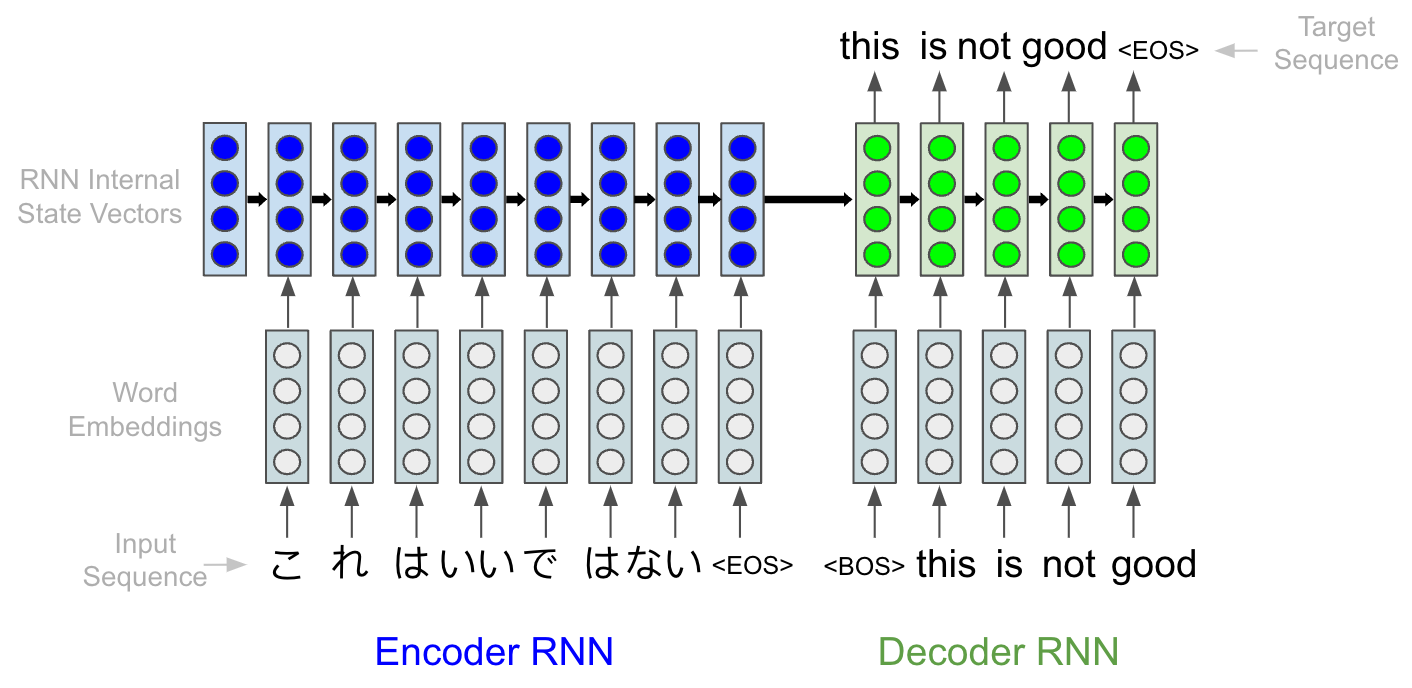
\includegraphics[width=5.5in]{figures/seq2seq-with-embeddings.png}
% \end{center}
% Each word is first turned into a vector embedding, then processed by the RNN.  The input sequence is the prompt, and the encoder RNN processes this input until it receives a special ``end of sequence'' (EOS) symbol.  The final state of the encoder RNN is then fed into the decoder RNN, which starts with the ``begin of sequence'' (BOS) symbol.  The decoder RNN is trained to output one word of the target sequence at each time step.  The output word at time $t$ is fed in as the input to the decoder RNN for time $t+1$, then the decoder RNN is used to generate the output word at time $t+1$.

% % problem with RNNs
% %
% % - need for complex patterns: towards multi-headed attention
% %
% %   - sentence that needs a long window
% %     Unlike the other white ducks in the pond, its feathers were _____
% %     Just like the other white ducks in the pond, its feathers were _____
% %
% %   - Not all words are important
% %     Judy needed to figure out how many pumpkins to buy for the party.
% %     Since twenty guests were coming and three could share one pumpkin, she decided to buy ______
% %
% %   - The important words may appear anywhere in the sentence
% %     Weather forcasts have clearly gotten much ______ since the since the game started 
% %     allowing magic users to abruptly change seasons in the fantasy world
% This can work pretty well for short prompts.  The challenge comes when the input sequence is long, because all the information about the prompt must be encoded in the final state of the encoder RNN.  And the state of an RNN typically becomes increasingly uncorrelated with a given input the further away it is in time.  For language translation, this is a pressing problem when the two languages have different grammar.  In Japanese, the sentiment of a sentence can be completely changed by the suffix added to the verb at the very end of the sentence.  This means that to accurately translate Japanese to English, the encoder RNN in our example needs to know both the initial and final Japanese words.  But the RNN will perform increasingly poorly as the input sentence gets longer.

% % seq2seq with attention
% Alternatively, an attention mechanism can be employed.  Conceptually, what we want is for the current state of the decoder RNN to be able to pay attention to a specific state vector of the encoder RNN, instead of just looking at the encoder RNN's final state.  For example, after outputting the word ``is,'' the decoder RNN in our Japanese translation scenario would want to know most about encoder RNN's state specifically at the word ``nai'' in the input, since that would generate the following English word in the output, ``not.''  We can accomplish this by employing the state of the encoder RNN as being both the keys and values, and letting the current state of the decoder RNN be the query, using this conceptual structure:
% \begin{center}
%   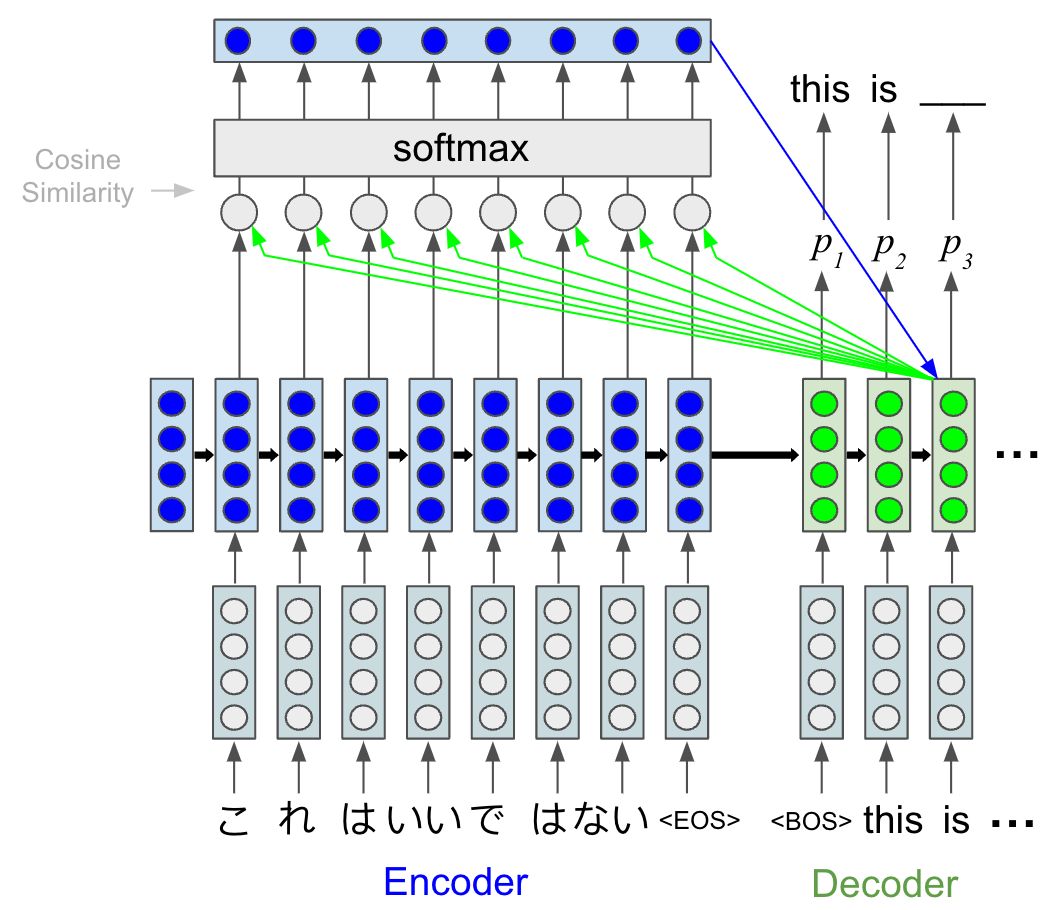
\includegraphics[width=4.615in]{figures/seq2seq-with-attention.png}
% \end{center}
% This is the conceptual structure of a seq2seq RNN with attention.  The top vector at the output of the softmax is the attention output, and this output is then used together with the decoder RNN's current state to produce the next output word.

% % patterns not based on spatial (CNN) or temporal (RNN) locality
% This usage of an attention mechanism bestows the RNNs with a kind of long-term memory, since generation of the output word can now utilize information from any word in the input sequence that is used to generate the attention output.  There are more sophisticated structures than the simple conceptual example given above.  For instance, the keys and values could use different vector embeddings, and an embedding could be applied to the values used to generate the attention output.  How the decoder employs the attention output to generate the next word can also be sophisticated.  And attention mechanisms are valuable not just for sequential data, but also for spatial data such as images.  Note that all of these embeddings and generation processes are generally neural networks that are trainable using back-propagation.  Actually training these embeddings can be difficult in practice, because of the large number of degrees of freedom, particularly as the number of keys and values grows.  But the main point to take away from this discussion is that attention mechanisms allows modeling of a far richer set of patterns than the temporally local RNN models, or even the spatially local CNN models, when applied to images.


% %%%%%%%%%%%%%%%%%%%%%%%%%%%%%%%%%%%%%%%%%%%%%%%%%%%%%%%%%%%%%%%%%%%%%%%%%%%%%




\subsection{Self Attention}
Self-attention is an attention mechanism where the keys, values, and queries are all generated from the same input.

At a very high level, typical transformer with self-attention layers maps $\mathbb{R}^{n\times d} \longrightarrow \mathbb{R}^{n\times d}$. In particular, the transformer takes in data (a sequence of tokens) $X\in \mathbb{R}^{n\times d}$ and for each token $x^{(i)}\in \mathbb{R}^{d\times 1}$, it computes (via learned projection, to be discussed in Section \ref{sec-learnedembedding}), a query $q_i \in \mathbb{R}^{d_q\times 1}$, key $k_{i} \in \mathbb{R}^{d_k\times 1}$, and value $v_{i} \in \mathbb{R}^{d_v\times 1}$. In practice, $d_q=d_k=d_v$ and we often denote all three embedding dimension via a unified $d_k.$\note{Note that $d_k$ differs from $d$: $d$ is the dimension of raw input token $\in \mathbb{R}^{d_q\times 1}$}

The self-attention layer then take in these query, key, and values, and compute a self-attention matrix
\begin{eqnarray}A = \begin{bmatrix}
    \text{softmax}\left( \begin{bmatrix}
                           q_1^\top k_1 & q_1^\top k_2 & \cdots & q_1^\top k_{n}
                         \end{bmatrix} / \sqrt{d_k} \right) \\
    \text{softmax}\left( \begin{bmatrix}
                           q_2^\top k_1 & q_2^\top k_2 & \cdots & q_2^\top k_{n}
                         \end{bmatrix} / \sqrt{d_k} \right) \\
    \vdots &                                                                   \\
    \text{softmax}\left( \begin{bmatrix}
                           q_{n}^\top k_1 & q_{n}^\top k_2 & \cdots & q_{n}^\top k_{n}
                         \end{bmatrix} / \sqrt{d_k} \right)
  \end{bmatrix}
\end{eqnarray}\label{eq:self_softmax}

Comparing this self-attention matrix with the attention matrix described in Equation \ref{eq:xfm_softmax}, we notice the only difference lies in the dimensions: since in self-attention, the query, key, and value all come from the same input, we have $n_q=n_k=n_v$, and we often denote all three with a unified $n$.

The self-attention output is then given by a weighted sum over the values:
$${y}^{(i)} = \sum_{j=1}^n  \alpha_{ij}
  v_{j}$$

This diagram below shows (only) the middle input token generating a query that is then combined with the keys computed with all tokens to generate the attention weights via a softmax. The output of the softmax is then combined with values computed from all tokens, to generate the attention output corresponding to the middle input token. Repeating this for each input token then generates the output.

% The idea is that for some input $x$, we generate a key $k = (W^k)^T x$ using a weight matrix $W^k$, a value $v = (W^v)^T x$ with weight matrix $W^v$, and a query using $(W^q)^T x$.  The attention mechanism then uses the attention function $\text{softmax}(q^T k)$ to determine which inputs are most relevant to a given $q$.  In the context of language translation example, this means that attention is used to determine which tokens (moving forward, let us think more generally, focusing on tokens instead of words) are most strongly related to each other.

\begin{center}
  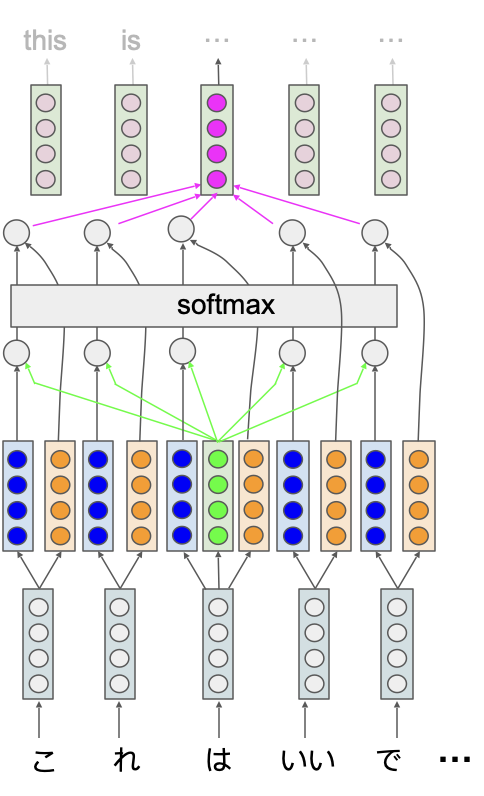
\includegraphics[width=2.615in]{figures/transformer-self-attention.png}
\end{center}



%  - output size same as input
%  - position encoding
%  - masking
\question{We have five colored tokens in the diagram above (gray, blue, organge, green, red). Could you read off the diagram the correspondence between the color and input, query, query, value, output? }

Note that the size of the output is the same as the size of the input.  Also, observe that there is no apparent notion of ordering of the input words in the depicted structure.  Positional information can be added by encoding a number for token (giving say, the token's position relative to the start of the sequence) into the vector embedding of each token.  And note that a given query need not pay attention to all other tokens in the input; in this example, the token used for the query is not used for a key or value.

% masking
More generally, a {\em mask} may be applied to limit which tokens are used in the attention computation.  For example, one common mask limits the attention computation to tokens that occur previously in time to the one being used for the query.  This prevents the attention mechanism from ``looking ahead'' in scenarios where the transformer is being used to generate one token at a time.

% % difference from RNN
% This single stage of self-attention is the principal component of a {\em transformer block}, and it is meaningfully different from an RNN: the transformer does not have a recurrent structure.  Thus, back-propagation-though-time does not need to be used, and the vanishing gradients problem of RNN's does not arise in the same way.  Moreover, all input tokens can be processed at once, instead of one at a time.  This means a transformer can be much faster to train than a comparable RNN: instead of requiring a number of training steps that grows linearly with the size of the input, the transformer can be trained in a single step, as long as sufficient computational resources are available for the parallel processing.

% multi-headed attention
Each self-attention stage is trained to have key, value, and query embeddings that lead it to pay specific attention to some particular feature of the input.  We generally want to pay attention to many different kinds of features in the input; for example, in translation one feature might be be the verbs, and another might be objects or subjects.  A transformer utilizes multiple instances of self-attention, each known as an ``attention head,'' to allow combinations of attention paid to many different features.

%%%%%%%%%%%%%%%%%%%%%%%%%%%%%%%%%%%%%%%%

\section{Transformers}
\label{sec-transformers}
A transformer is the composition of a number of transformer blocks, each of which has multiple attention heads. At a very high-level, the goal of a transformer block is to output a really rich, useful representation for each input token, all for the sake of being high-performant for whatever task the model is trained to learn.

Rather than depicting the transformer graphically, it is worth returning to the beauty of the underlying equations\footnote{The presentation here follows the notes by John Thickstun.}.





% formal definition
%
% Mathematical summary, following John Thickstun, but rewritten in 6.390 standard notation
% 6.390 conventions are that
% data input = d x n (each column is a data vector)
% superscript x^{(i)} indicates sample number
% NN output is W^T X
% need to include heads
%
% layer norm?
% residual connections?
%

%
\subsection{Learned embedding}\label{sec-learnedembedding}
For simplicity, we assume the transformer internally uses self-attention. Full general attention layers work out similarly.

Formally, a transformer block is a parameterized function $f_\theta$ that maps $\R^{n\times d}\rightarrow \R^{n\times d}$, where the input data $X \in \R^{n\times d}$ is often represented as a sequence of $n$ tokens, with each token $x^{(i)}\in \mathbb{R}^{d\times 1}.$


Three projection matrices (weights) $W_{q}, W_k, W_v$ are to be learned, such that, for each token $x^{(i)}\in \mathbb{R}^{d\times 1}$, we produce 3 distinct vectors: a query vector $q_i = W_q^T x^{(i)}$; a key vector $k_i = W_k^T x^{(i)}$; a value vector $v_i = W_v^T x^{(i)},$ all 3 of these vectors $\mathbb{R}^{d_k\times 1}$ and the learned weights $W_{q}, W_{k}, W_{v} \in \R^{d\times d_k}.$

If we stack these $n$ query, key, value vectors into matrix- form, such that $Q\in \mathbb{R}^{n\times d_k}$, $K\in \mathbb{R}^{n\times d_k}$, and $V\in \mathbb{R}^{n\times d_k},$ then we can more compactly write out the learned transformation from the sequence of input token $X$:
\begin{eqnarray*}
  Q &=& X W_{q}
  \\
  K &=& X W_{k}
  \\
  V &=& X W_{v}
\end{eqnarray*}
These $Q, K, V$ triple can then be used to produce one (self)attention-layer output. One such layer is called one "attention head".

One can have more than one "attention head", such that: the queries, keys, and values are embedded via encoding matrices:
\begin{eqnarray}
  Q^{(h)} &=& X W_{h,q}
  \\
  K^{(h)} &=& X W_{h,k}
  \\
  V^{(h)} &=& X W_{h,v}
\end{eqnarray}
and $W_{h,q}, W_{h,k}, W_{h,v} \in \R^{d\times d_k}$where $d_k$ is the size of the key/query embedding space, and $h \in \{1,\cdots,H\}$ is an index over ``attention heads.'' \note{for each attention-head $h$, we learn one set of $W_{h,q}, W_{h,k}, W_{h,v}$.}

We then perform a weighted sum over all the outputs for each head,
\begin{eqnarray}
  {u'}^{(i)} = \sum_{h=1}^H W^T_{h,c} \sum_{j=1}^{n} \alpha^{(h)}_{ij} V^{(h)}_j
  \,,
\end{eqnarray}

where $W_{h,c} \in \R^{d_k\times d},$ ${u'}^{(i)} \in \R^{d\times 1},$ the indices $i \in \{1,\cdots,n\}$ and $j \in \{1,\cdots,n\}$ are an integer index over tokens. \note{$V^{(h)}_j$ is the $d_k\times 1$ value embedding vector that corresponds to the input token $x^{j}$ for attention head $h$.}

This is then standardized and combined with $x^{(i)}$ using a $\text{LayerNorm}$ function (defined below) to become
\begin{eqnarray}
  {u}^{(i)} = \text{LayerNorm}\left(  x^{(i)} + {u'}^{(i)}; \gamma_1, \beta_1  \right)
\end{eqnarray}
with parameters $\gamma_1, \beta_1 \in \R^{d}$.

To get the final output, we follow the ``intermediate output then layer norm" recipe again. In particular, we first get the transformer block output ${z'}^{(i)}$ given by
\begin{eqnarray}
  {z'}^{(i)} = W_2^T \text{ReLU}\left( W_1^T u^{(i)} \right)
\end{eqnarray}
with weights $W_1\in \R^{d\times m}$ and $W_2\in \R^{m\times d}$.  This is then standardized and combined with $u^{(i)}$ to give the final output $z^{(i)}$:
\begin{eqnarray}
  {z}^{(i)} = \text{LayerNorm}\left(  u^{(i)} + {z'}^{(i)}; \gamma_2, \beta_2  \right)
  \,,
\end{eqnarray}
with parameters $\gamma_2, \beta_2 \in \R^{d}$.  These vectors are then assembled (e.g., through parallel computation) to produce $z\in \R^{n\times d}$.

The $\text{LayerNorm}$ function transforms a $d$-dimensional input $z$ with parameters $\gamma, \beta \in \R^d$ into
\begin{eqnarray}
  \text{LayerNorm}(z; \gamma, \beta) = \gamma \frac{z-\mu_z}{\sigma_z} + \beta
  \,,
\end{eqnarray}
where $\mu_z$ is the mean and $\sigma_z$ the standard deviation of $z$:
\begin{eqnarray}
  \mu_z &=& \frac{1}{d} \sum_{i=1}^d z_i
  \\
  \sigma_z &=& \sqrt{ \frac{1}{d} \sum_{i=1}^d (z_i-\mu_z)^2 }
  \,.
\end{eqnarray}
Layer normalization is done to improve convergence stability during training.

The model parameters comprise the weight matrices $W_{h,q}, W_{h,k}, W_{h,v}, W_{h,c}, W_1, W_2$ and the $\text{LayerNorm}$ parameters $\gamma_1, \gamma_2, \beta_1, \beta_2$.  A {\em transformer} is the composition of $L$ transformer blocks, each with its own parameters:
\begin{eqnarray}
  f_{\theta_L} \circ  \cdots \circ f_{\theta_2} \circ f_{\theta_1}(x) \in \R^{n\times d}
  \,.
\end{eqnarray}
The hyperparameters of this model are $d, d_k, m, H,$ and $L.$


% (where typically $d=512$, $d_k = 64$, $m=2048$, $H=8$, and $L\ge 6$.


%%%%%%%%%%%%%%%%%%%%%%%%%%%%%%%%%%%%%%%%
\subsection{Variations and training}

Many variants on this transformer structure exist.  For example, the $\text{LayerNorm}$ may be moved to other stages of the neural network.  Or a more sophisticated attention function may be employed instead of the simple dot product used in Eq.~\ref{eq:xfm_softmax}.  Transformers may also be used in pairs, for example, one to process the input and a separate one to generate the output given the transformed input.  Self-attention may also be replaced with cross-attention, where some input data are used to generate queries and other input data generate keys and values.  Positional encoding and masking are also common, though they are left implicit in the above equations for simplicity.

How are transformers trained?  The number of parameters in $\theta$ can be very large; modern transformer models like GPT4 have tens of billions of parameters or more.  A great deal of data is thus necessary to train such models, else the models may simply overfit small datasets.

Training large transformer models is thus generally done in two stages.  A first ``pre-training'' stage employs a very large dataset to train the model to extract patterns.  This is done with unsupervised (or self-supervised) learning and unlabelled data.  For example, the well-known BERT model was pre-trained using sentences with words masked.  The model was trained to predict the masked words.  BERT was also trained on sequences of sentences, where the model was trained to predict whether two sentences are likely to be contextually close together or not. The pre-training stage is generally very expensive.

The second ``fine-tuning'' stage trains the model for a specific task, such as classification or question answering.  This training stage can be relatively inexpensive, but it generally requires labeled data.





\chapter{Non-parametric methods}
\label{chap-nonparametric}

Neural networks have adaptable complexity, in the sense that we can
try different structural models and use cross validation to find one
that works well on our data.  Beyond neural networks, we may further
broaden the class of models that we can fit to our data, for example
as illustrated by the techniques introduced in this chapter.

Here, we turn to models that automatically adapt their complexity to
the training data.  The name {\em non-parametric
    methods}\index{non-parametric methods} is misleading: it is really a
class of methods that does not have a fixed parameterization in
advance.  Rather, the complexity of the parameterization can grow as
we acquire more data.

Some non-parametric models, such as nearest-neighbor, rely directly on the
data to make predictions and do not compute a model that summarizes
the data. Other non-parametric methods, such as decision trees\note{These are sometimes called {\em classification trees}; the decision analysis literature uses ``decision tree'' for a structure that lays out possible future events that consist of choices interspersed with chance nodes.},
can be seen as
dynamically constructing something that ends up looking like a more
traditional parametric model, but where the actual training data
affects exactly what the form of the model will be.

The non-parametric methods we consider here tend to have the form of a
composition of simple models:
\begin{itemize}
  \item{\em Nearest neighbor models}: (Section~\ref{sec-np_nn}) where we
        don't process data at training time, but do all the work when making
        predictions, by looking for the closest training example(s) to a given
        new data point.\index{nearest neighbor models}
  \item {\em Tree models}: (Section~\ref{sec-np_trees}) where we
        partition the input space and use different simple predictions on
        different regions of the space; the hypothesis space can become
        arbitrarily large allowing finer and finer partitions of the
        input space.\index{tree models}
  \item {\em Ensemble models}: (Section~\ref{sec-np_bagging}) in which
        we train several different classifiers on the whole space and
        average the answers; this decreases the estimation
        error.\index{ensemble models} In particular, we will look at
        bootstrap aggregation, or {\em bagging} of trees.
  \item{\em Boosting}\index{boosting} is a way to construct a model
        composed of a sequence of component models (e.g., a model consisting of
        a sequence of trees, each subsequent tree seeking to correct
        errors in the previous trees) that decreases both estimation and
        structural error. We won't consider this in detail in this class.
\end{itemize}

\medskip
Why are we studying these methods, in the heyday of complicated models such as neural networks%(which we will see next week)
?
\begin{itemize}
  \item They are fast to implement and have few or no hyperparameters
        to tune.
  \item They often work as well as or better than more complicated methods.
  \item Predictions from some of these models can be easier to explain
        to a human user: decision trees are fairly directly
        human-interpretable, and nearest neighbor methods can justify their
        decision to some extent by showing a few training examples that the
        prediction was based on.
\end{itemize}

%%%%%%%%%%%%%%%%%%%%%%%%%%%%%%%%%%%%%%%%%%%%%%%%%%%%%%%%%%%%%%%%%%%%%%%%%%%%%

\section{Nearest Neighbor}
\label{sec-np_nn}

In nearest-neighbor models, we don't do any processing of the data at
training time -- we just remember it!  All the work is done at
prediction time.

Input values $x$ can be from any domain $\mathcal X$ ($\R^d$, documents,
tree-structured objects, etc.).
We just need a distance metric, $d: \mathcal X \times \mathcal X
  \rightarrow \R^+$, which satisfies the following, for all $x, x', x'' \in
  \mathcal X$:
\begin{align*}
  d(x, x)   & = 0                        \\
  d(x, x')  & = d(x', x)                 \\
  d(x, x'') & \leq d(x, x') + d(x', x'')
\end{align*}

Given a data-set $\data = \{(\ex{x}{i},\ex{y}{i})\}_{i=1}^n$, our
predictor for a new $x \in \mathcal X$ is
\begin{equation}
  h(x) = \ex{y}{i} \;\;\;\text{where}\;\;\;i = \argmin{i} d(x,
  \ex{x}{i})\;\;,
\end{equation}
that is, the predicted output associated with the training point that
is closest to the query point $x$. Tie breaking is typically done at random.

This same algorithm works for regression {\em and} classification!

The nearest neighbor prediction function can be described by dividing
the space up into regions whose closest point is each individual training
point as shown below \note{Decision boundary regions can also be described
  by Voronoi diagrams. In a Voronoi diagram, each of the data points would have
  its own ``cell'' or region in the space that is closest to the data point in question.
  In the diagram provided here, cells have been merged if the predicted value is the
  same in adjacent cells.}:
\begin{center}
  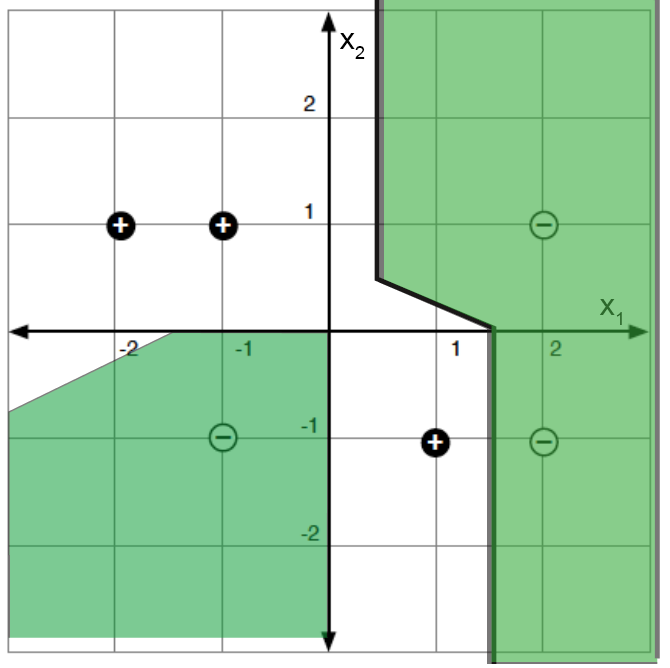
\includegraphics[scale=0.75]{figures/voronoi.png}
\end{center}
In each region, we predict the associated $y$ value.
\question{Convince yourself that these boundaries do represent the
  nearest-neighbor classifier derived from these six data points.}

There are several useful variations on this method.  In {\em
    $k$-nearest-neighbors}, we find the $k$  training points nearest to
the query point $x$ and output the majority $y$ value for
classification or the average for regression.  We can also do {\em
    locally weighted regression} in which we fit locally linear
regression models to the $k$ nearest points, possibly giving less
weight to those that are farther away.  In large data-sets, it is
important to use good data structures (e.g., ball trees) to perform
the nearest-neighbor look-ups efficiently (without looking at all the
data points each time).

\section{Tree Models}
\label{sec-np_trees}

The idea here is that we would like to find a partition of the input
space and then fit very simple models to predict the output in each
piece.  The partition is described using a (typically binary)
``tree'' that recursively splits the space.

\medskip
Tree methods differ by:
\begin{itemize}
  \item The class of possible ways to split the space at each node;
        these are typically linear splits, either aligned with the axes of
        the space, or sometimes using more general classifiers.
  \item The class of predictors within the partitions; these are often
        simply constants, but may be more general classification or
        regression models.
  \item The way in which we control the complexity of the hypothesis: it
        would be within the capacity of these methods to have a separate
        partition element for each individual training example.
  \item The algorithm for making the partitions and fitting the models.
\end{itemize}

One advantage of tree models is that they are easily interpretable by
humans.  This is important in application domains, such as medicine,
where there are human experts who often ultimately make critical
decisions and who need to feel confident in their understanding of
recommendations made by an algorithm. Below is an example decision
tree, illustrating how one might be able to understand the
decisions made by the tree.
\medskip

\begin{examplebox}{\bf Example:}
  Here is a sample tree (reproduced from Breiman, Friedman, Olshen, Stone (1984)):

  \tikzstyle{vertex}=[draw,fill=black!15,rectangle,minimum size=20pt,inner sep=6pt]
  \tikzstyle{leafgreen}=[draw,fill=green!15,rectangle,minimum size=20pt,inner sep=6pt]
  \tikzstyle{leafred}=[draw,fill=red!15,rectangle,minimum size=20pt,inner sep=6pt]

  \begin{center}
    \begin{tikzpicture}[very thick,level distance=2.05cm,level 1/.style={sibling distance=40mm},level 2/.style={sibling distance=5cm}]
      \node [vertex] (r){\begin{minipage}{14em}{\begin{center}Minimum systolic blood pressure over 24h period $\geq$ 91?\end{center}}\end{minipage}}
      child {
          node [leafred] (a) {high risk}
          edge from parent node[left,draw=none,xshift=-0.4pt,yshift=3pt] {no}
        }
      child {
          node [vertex] {Age $\geq$ 65?}
          child {
              node [leafgreen] {low risk}
              edge from parent node[left,draw=none,xshift=-0.4pt,yshift=3pt] {no}
            }
          child {
              node [vertex] {\begin{minipage}{9em}{\begin{center}Is sinus tachycardia present?\end{center}}\end{minipage}}
              child {node [leafgreen] {low risk}
                  edge from parent node[left,draw=none,xshift=-0.4pt,yshift=3pt] {no}
                }
              child {node [leafred] {high risk}
                  edge from parent node[right,draw=none,xshift=-0.0pt,yshift=2pt] {yes}
                }
              edge from parent node[right,draw=none,xshift=-0.0pt,yshift=2pt] {yes}
            }
          edge from parent node[right,draw=none,xshift=-0.0pt,yshift=2pt] {yes}
        };
    \end{tikzpicture}
  \end{center}

\end{examplebox}

These methods are most appropriate for domains where the input space
is not very high-dimensional and where the individual input features
have some substantially useful information individually or in small
groups.  Trees would not be good for image input, but might
be good in cases with, for example, a set of meaningful measurements
of the condition of a patient in the hospital, as in the example
above.

We'll concentrate on the CART/ID3 (``classification and regression
trees'' and ``iterative dichotomizer 3'', respectively) family of
algorithms, which were invented independently in the statistics and
the artificial intelligence communities.  They work by greedily
constructing a partition, where the splits are {\em axis aligned} and
by fitting a {\em constant} model in the leaves.  The interesting
questions are how to select the splits and how to control complexity.
The regression and classification versions are very similar.

As a concrete example, consider the following images:
\begin{center}
  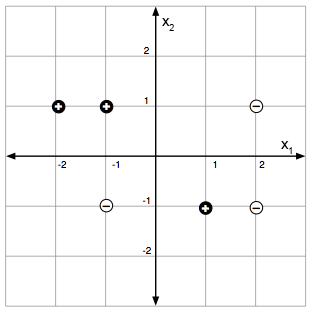
\includegraphics[scale=1]{figures/dt_points.png}
  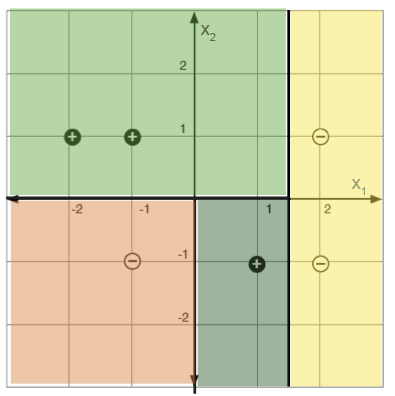
\includegraphics[scale=1]{figures/dt_soln.png}
\end{center}
The left image depicts a set of labeled data points in a two-dimensional
feature space. The right shows a partition into regions by a decision
tree, in this case having no classification errors in the final
partitions.


\subsection{Regression}\index{tree models!regression tree}

\def\Rfeat{R}
\def\Rdata{\hat{R}}

The predictor is made up of
\begin{itemize}
  \item a partition function, $\pi$, mapping elements of the input space into
        exactly one of $M$ regions, $\Rfeat_1, \ldots, \Rfeat_M$, and
  \item a collection of $M$ output values, $O_m$, one for each region.
\end{itemize}

If we already knew a division of the space into regions, we would set
$O_m$, the constant output for region $\Rfeat_m$, to be the average of
the training output values in that region.
For a training data set $\data = \left\{\left(\ex{x}{i},
  \ex{y}{i}\right)\right\}, i = 1, \ldots n$, we let ${\emph I}$ be an indicator
set of all of the elements within $\data$, so that ${\emph I} = \{1, \ldots, n\}$ for
our whole data set.
We can define ${\emph I}_m$ as the subset of data set samples that are
in region $R_m$, so that ${\emph I}_m = \{ i \mid \ex{x}{i} \in R_m\}$. Then
$$O_m = {\rm average}_{i \in {\emph I}_m}~\ex{y}{i}\;\;.$$
We can define the error in a region as $E_m$. For example,
$E_m$ as the sum of squared error would be expressed as
\begin{equation}
  E_m = \sum_{i \in {\emph I}_m}(\ex{y}{i} - O_m)^2\;\;.
\end{equation}
Ideally, we would select the partition to minimize
\begin{equation}
  \lambda M + \sum_{m=1}^M E_m\;\;,
\end{equation}
for some regularization constant $\lambda$.  It is enough to search over all
partitions of the training data (not all partitions of the input
space!) to optimize this, but the problem is NP-complete.
\question{Be sure you understand why it's enough to consider all
  partitions of the training data, if this is your objective.}

\subsubsection{Building a tree}\index{tree models!building a tree}
So, we'll be greedy.  We establish a criterion, given a set of data,
for finding the best single split of that data, and then apply it
recursively to partition the space.  For the discussion below, we
will select the partition of
the data that {\em minimizes the sum of the sum of squared errors of
    each partition element.} Then later, we will consider other
splitting criteria.

Given a data set $\data = \left\{\left(\ex{x}{i},
  \ex{y}{i}\right)\right\}, i = 1, \ldots n$, we now consider ${\emph I}$ to be an indicator
of the subset of elements within $\data$ that we wish to build a tree (or subtree) for.
That is, ${\emph I}$ may already indicate a subset of data set $\data$, based on
prior splits in constructing our overall tree. We define terms as follows:

%% \note{A small subtlety: $\Rdata^+_{j,s}$ is a subset of data, but $\Rfeat_m$ is a partition of the feature space.}

\begin{itemize}
  \item ${\emph I}^+_{j,s}$ indicates the set of examples (subset of
        ${\emph I}$) whose feature value in dimension $j$ is greater than or
        equal to split point $s$;
  \item ${\emph I}^-_{j,s}$ indicates the set of examples (subset of
        ${\emph I}$) whose feature value in dimension $j$ is less than $s$;
  \item $\hat{y}^+_{j,s}$ is the average $y$ value of the data points
        indicated by set ${\emph I}^+_{j,s}$; and
  \item $\hat{y}^-_{j,s}$ is the average $y$ value of the data points
        indicated by set ${\emph I}^-_{j,s}$.
\end{itemize}

Here is the pseudocode. In what follows, $k$ is the largest leaf
size that we will allow in the tree, and is a hyperparameter of the algorithm.
\begin{codebox}
  \Procname{$\proc{BuildTree}({\emph I}, k)$}
  \li  \If $|{\emph I}| \leq k$
  \Then
  \li    Set $\hat{y} = {\rm average}_{i \in {\emph I}}~\ex{y}{i}$
  \li    \Return $\proc{Leaf}({\rm value} = \hat{y})$
  \li  \Else
  \li   \For each split dimension $j$ and split value $s$
  \li     \Do
  Set ${\emph I}^+_{j,s} = \{i \in {\emph I} \mid x_j^{(i)} \geq s\}$
  \li Set ${\emph I}^-_{j,s} = \{i \in {\emph I} \mid x_j^{(i)} < s\}$
  \li Set $\hat{y}^+_{j,s} = {\rm average}_{i \in {\emph I}^+_{j,s}} ~ \ex{y}{i}$
  \li Set $\hat{y}^-_{j,s} = {\rm average}_{i \in {\emph I}^-_{j,s}} ~ \ex{y}{i}$
  \li Set $E_{j,s} = \sum_{i \in {\emph I}^+_{j,s}} (\ex{y}{i} - \hat{y}^+_{j,s})^2 +
    \sum_{i \in {\emph I}^-_{j,s}} (\ex{y}{i} - \hat{y}^-_{j,s})^2$
  \End
  \li        Set $(j^*, s^*) = {\rm arg~min}_{j,s} E_{j,s}$
  \End
  \li    \Return $\proc{Node}(j^*, s^*, \proc{BuildTree}({\emph I}^-_{j^*, s^*}, k), \proc{BuildTree}({\emph I}^+_{j^*, s^*}, k))$
\end{codebox}

In practice, we typically start by calling $\proc{BuildTree}$ with the first
input equal to our
whole data set (that is, with ${\emph I} = \{1,\ldots,n\}$). But then that
call of $\proc{BuildTree}$ can recursively lead to many other calls
of $\proc{BuildTree}$.

Let's think about how long each call of $\proc{BuildTree}$ takes to
run. We have to consider all possible splits. So we consider a split
in each of the $d$ dimensions. In each dimension, we only need to
consider splits between two data points (any other split will give the
same error on the training data). So, in total, we consider $O(d n)$
splits in each call to $\proc{BuildTree}$.
\question{Concretely, what would
  be a good set of split-points to consider for dimension $j$ of a
  data set indicated by ${\emph I}$?}

\subsubsection{Pruning}\index{tree models!pruning}
It might be tempting to regularize by using a somewhat large
value of $k$, or by stopping when splitting a node does not significantly
decrease the error.  One problem with short-sighted stopping criteria
is that they might not see the value of a split that will require one
more split before it seems useful.
\question{Apply the decision-tree algorithm to the XOR problem in two
  dimensions.  What is the training-set error of all possible
  hypotheses based on a single split?}
So, we will tend to build a tree that is too large, and then prune it
back.

We define {\em cost complexity}\index{tree models!cost complexity} of a
tree $T$, where $m$ ranges over its leaves, as
\begin{equation}
  C_\alpha(T) = \sum_{m = 1}^{|T|} E_m(T) + \alpha |T|\;\;,
\end{equation}
and $|T|$ is the number of leaves.
For a fixed $\alpha$, we can find a $T$ that (approximately) minimizes
$C_\alpha(T)$ by ``weakest-link'' pruning:
\begin{itemize}
  \item Create a sequence of trees by successively removing the
        bottom-level split that minimizes the increase in overall error,
        until the root is reached.
  \item Return the $T$ in the sequence that minimizes the cost complexity.
\end{itemize}
We can choose an appropriate $\alpha$ using cross validation.

\subsection{Classification}\index{tree models!classification}

The strategy for building and pruning classification trees is very
similar to the strategy for regression trees.

Given a region $\Rfeat_m$ corresponding to a leaf of the tree, we would
pick the output class $y$ to be the value that exists most frequently
(the {\em majority value}) in the data points whose $x$ values are in
that region, i.e., data points indicated by ${\emph I}_m$:
$$O_m = {\rm majority}_{i \in {\emph I}_m}~\ex{y}{i}\;\;.$$
Let's now define the error in a region as the number of data points that do not
have the value $O_m$:
$$E_m = \left|\{i \mid i \in {\emph I}_m \;\text{and}\; \ex{y}{i} \not
  = O_m\}\right|\;\;.$$
We define the {\em empirical probability}\index{empirical probability} of an item from class $k$
occurring in region $m$ as:
\[\hat{P}_{m,k} = \hat{P}({\emph I}_m,k) = \frac{\left|\{i \mid i \in {\emph I}_m
    \;\text{and}\; \ex{y}{i} = k\}\right|}{N_m}\;\;,\] where
$N_m$ is the number of training points in region $m$; that is, $N_m = |{\emph I}_m|.$
For later use, we'll also define the empirical probabilities of split values,
$\hat{P}_{m,j,s}$, as the fraction of points with dimension $j$ in
split $s$ occurring in region $m$ (one branch of the tree), and $1 -
  \hat{P}_{m,j,s}$ as the complement (the fraction of points in the
other branch).

\paragraph*{Splitting criteria}\index{tree models!splitting criteria}
In our greedy algorithm, we need a way to decide which split to make
next.  There are many criteria that express some measure of the
``impurity'' in child nodes.  Some measures include:
\begin{itemize}
  \item {\em Misclassification error}:\index{tree models!splitting criteria!misclassification error}
        \begin{equation}
          Q_m(T) = \frac{E_m}{N_m} = 1 - \hat{P}_{m,O_m}
        \end{equation}
  \item {\em Gini index}:\index{tree models!splitting criteria!Gini index}
        \begin{equation}
          Q_m(T) = \sum_k \hat{P}_{m,k}(1 - \hat{P}_{m,k})
        \end{equation}
  \item {\em Entropy}: \index{tree models!splitting criteria!entropy}
        \begin{equation}
          Q_m(T) = H({\emph I}_m) = - \sum_k \hat{P}_{m,k} \log_2 \hat{P}_{m,k}
        \end{equation}
        So that the entropy $H$ is well-defined when $\hat{P} = 0$, we will stipulate that $0 \log_2 0 = 0$.
\end{itemize}
These splitting criteria are very similar, and it's not entirely obvious which one is
better.  We will focus on entropy, just to be concrete.

Analogous to how for regression we choose the dimension $j$ and split
$s$ that minimizes the sum of squared error $E_{j,s}$, for
classification, we choose the dimension $j$ and split $s$ that
minimizes the weighted average entropy over the ``child'' data points
in each of the two corresponding splits,
${\emph I}^+_{j,s}$ and ${\emph I}^-_{j,s}$.
We calculate the entropy in each split based on the
empirical probabilities of class memberships in the split, and then
calculate the weighted average entropy $\hat{H}$ as
\begin{align}
  \hat{H} & = \text{(fraction of points in left data set)} \cdot H(I_{j,s}^-) \nonumber                     \\
          & \qquad + \text{(fraction of points in right data set)} \cdot H(I_{j,s}^+) \nonumber             \\
          & = (1-\hat{P}_{m,j,s}) H({\emph I}_{j,s}^{-}) + \hat{P}_{m,j,s} H({\emph I}_{j,s}^{+}) \nonumber \\
          & = \frac{|I^-_{j,s}|}{N_m} \cdot H(I_{j,s}^-) + \frac{|I^+_{j,s}|}{N_m} \cdot H(I_{j,s}^+)\; .
\end{align}
Choosing the split that minimizes the entropy of the children is
equivalent to maximizing the {\em information gain}\index{tree
  models!information gain} of the test $x_j = s$, defined by
\begin{eqnarray}
  \proc{infoGain}(x_j = s, {\emph I}_m) & = & H({\emph I}_m) -
  \left(\frac{|I^-_{j,s}|}{N_m} \cdot H(I_{j,s}^-) + \frac{|I^+_{j,s}|}{N_m} \cdot H(I_{j,s}^+)\right)
\end{eqnarray}

In the two-class case (with labels 0 and 1), all of the splitting criteria mentioned
above have the values
\[
  \begin{cases}
    0.0 & \text{when $\hat{P}_{m,0} = 0.0$} \\
    0.0 & \text{when $\hat{P}_{m,0} = 1.0$}
  \end{cases} \; .
\]
The respective impurity curves are shown below, where $p =
  \hat{P}_{m,0}$; the vertical axis plots $Q_m(T)$ for each of the three
criteria.
\begin{center}
  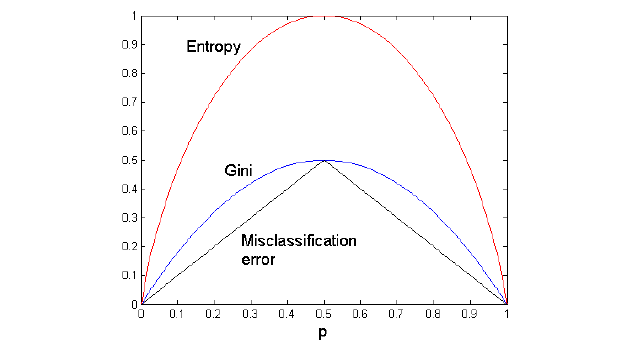
\includegraphics[scale=0.5]{figures/impurity.png}
\end{center}
There used to be endless haggling about which impurity function one should
use.  It seems to be traditional to use {\em entropy} to select which
node to split while growing the tree, and {\em misclassification error}
in the pruning criterion.


\subsection{Bagging}\index{bagging}
\label{sec-np_bagging}

One important limitation or drawback in conventional trees is
that they can have high estimation error: small changes in the data
can result in very big changes in the resulting tree.

  {\em Bootstrap aggregation} is a technique for reducing the estimation
error of a non-linear predictor, or one that is adaptive to the
data. The key idea applied to trees, is to build multiple
trees with different subsets of the data, and then create an ensemble
model that combines the results from multiple trees to make a
prediction.

\begin{itemize}
  \item Construct $B$ new data sets of size $n$. Each data set
        is constructed by sampling $n$ data points with replacement from $\data$.
        A single data set is called {\em bootstrap sample} of $\data$.
  \item Train a predictor $\hat{f}^b(x)$ on each bootstrap sample.
  \item {\em Regression case}:  bagged predictor is
        \begin{equation}
          \hat{f}_{\rm bag}(x) = \frac{1}{B} \sum_{b=1}^B \hat{f}^b(x) \; .
        \end{equation}

  \item {\em Classification case}:  Let $K$ be the number of classes. We
        find a majority bagged predictor as follows. We let
        $\hat{f}^b(x)$ be a ``one-hot'' vector with a single 1 and $K-1$ zeros,
        and define the predicted output $\hat{y}$ for predictor $f^b$ as
        $\hat{y}^b(x) = \argmax{k} \hat{f}^b(x)_k$.  Then
        \begin{equation}
          \hat{f}_{\rm bag}(x) = \frac{1}{B} \sum_{b=1}^B \hat{f}^b(x),
        \end{equation}
        which is a vector containing the proportion of classifiers that
        predicted each class $k$ for input $x$. Then the overall predicted output is
        \begin{equation}
          \hat{y}_{\rm bag}(x) = \argmax{k} \hat{f}_{\rm bag}(x)_k\;\;.
        \end{equation}

        % Alternatively, we can average the class probabilities from the
        % individual classifier, which gives us an even lower-variance estimate.
\end{itemize}

There are theoretical arguments showing that bagging does, in fact,
reduce estimation error.  However, when we bag a model, any simple
intrepetability is lost.
% In the case of regression and {\em squared error}, we can show that
% expected squared error of a classifier trained on a single data set of
% size $n$ is bounded below by the squared error of a classifier that is
% an average over classifiers trained on infinitely many data sets of
% size $n$ {\em drawn from the population}.  This suggests that bagging
% (in which new training sets are drawn from the data set, not
% population) will also decrease error.

% For classification under 0-1 loss, bagging can improve a good
% classifier, but it can also make a bad classifier worse.  
% But, here's a way to understand its advantage:\note{From Dietterich,
%   via Hastie, Tibshirani, and Friedman.}
% \begin{itemize}
% \item Let the Bayes optimal decision at $x$ be $Y(x) = 1$ in a
%   two-class example.
% \item Suppose each ``committee member'' $Y_b$ has an error rate $e_b <
% e < 0.5$ 
% \item Let $S_1(x) = \sum_{b=1}^B I(G_b(x) = 1)$ be the number of votes
%   for class 1 given input $x$
% \item If the committee members are independent, $S_1(x) \sim {\rm
%     Bin}(B, 1-e)$ and so $\Pr(S_1 > B/2) \rightarrow 1$ as $B$ gets large.
% \note{This is the ``Wisdom of Crowds.''}
% \end{itemize}
% The main issue with this analysis is that it assumes the committee
% members are independent, which they definitely are not in this
% case.


\subsection{Random Forests}

Random forests are collections of trees that are constructed to be
de-correlated, so that using them to vote gives maximal advantage.
In competitions, they often have excellent classification performance
among large collections of much fancier methods.

In what follows, $B$, $m$, and $n$ are hyperparameters of the algorithm.

\begin{codebox}
  \Procname{$\proc{RandomForest}(\data; B, m, n)$}
  \li  \For $b = 1, \ldots, B$
  \Do
  \li    Draw a bootstrap sample $\data_b$ of size $n$ from $\data$
  \li    Grow a tree $T_b$ on data $\data_b$ by recursively:
  \Do
  \li      Select $m$ variables at random from the $d$ variables
  \li      Pick the best variable and split point among the $m$ variables
  \li      Split the node
  \End
  \End
  \li   \Return tree $T_b$
\end{codebox}
Given the ensemble of trees, vote to make a prediction on a new $x$.

\subsection{Tree variants and tradeoffs}

There are many variations on the tree theme. One is to employ
different regression or classification methods in each leaf.  For
example, a linear regression might be used to model the examples in
each leaf, rather than using a constant value.

In the relatively simple trees that we've considered, splits
have been based on only a single feature at a time, and with the
resulting splits being axis-parallel. Other methods for splitting are
possible, including consideration of multiple features and linear
classifiers based on those, potentially resulting in non-axis-parallel
splits. Complexity is a concern in such cases, as many possible
combinations of features may need to be considered, to select the
best variable combination (rather than a single split variable).

Another generalization is a {\em hierarchical mixture of experts},
where we make a ``soft'' version of trees, in which the splits are
probabilistic (so every point has some degree of membership in every
leaf). Such trees can be trained using a form of gradient
descent. Combinations of bagging, boosting, and mixture tree
approaches (e.g., {\em gradient boosted trees}) and
implementations are readily available (e.g., XGBoost).

Trees have a number of strengths, and remain a valuable tool
in the machine learning toolkit.  Some benefits include being
relatively easy to interpret, fast to train, and ability to handle
multi-class classification in a natural way. Trees can easily
handle different loss functions; one just needs to change the
predictor and loss being applied in the leaves. Methods also exist to
identify which features are particularly important or influential in
forming the tree, which can aid in human understanding of the data
set.  Finally, in many situations, trees perform surprisingly
well, often comparable to more complicated regression or
classification models. Indeed, in some settings it is considered good
practice to start with trees (especially random forest or
boosted trees) as a ``baseline'' machine learning model,
against which one can evaluate performance of more sophisticated
models.



%%%%%%%%%%%%%%%%%%%%%%%%%%%%%%%%%%%%%%%%%%%%%%%%%%%%%%%%%%%%%%%%%%%%%%%%%%%%%





%%% Local Variables:
%%% mode: latex
%%% TeX-master: "top"
%%% End:

\chapter{Markov Decision Processes}
\label{chap-mdps}
So far, most of the learning problems we have looked at have been {\em supervised}, that is, for each training input $\ex{x}{i}$, we
are told which value $\ex{y}{i}$ should be the output. From a traditional machine-learning viewpoint, there're two other major groups of learning problems: one is the {\em unsupervised} learning problems, in
which we are given data and no expected outputs, and we will look at later in Chapter \ref{chap-clustering} and Chapter \ref{chap-autoencoders}.

The other major type is the so-called {\em Reinforcement learning}\index{reinforcement learning} (RL) problems. Reinforcement learning differs significantly from supervised learning problems, and we will delve into the details later in in Chapter \ref{chap-reinforcement}. However, it's worth pointing out one major difference at a very high level: in supervised learning, our goal is to learn a one-time static mapping to make predictions, whereas in RL, the setup requires us to sequentially take actions to maximize cumulative rewards.

This setup change necessitates additional mathematical and algorithmic tools for us to understand RL. {\em Markov decision process}\index{Markov decision process} ({\sc mdp}) is precisely such a classical and fundamental tool.


%%%%%%%%%%%%%%%%%%%%%%%%%%%%%%%%%%%%%%%%%%%%%%%%%%%%%%%%%%%%%%%%%%%%%%%%%%%%%

\section{Definition and value functions}
\label{sec_mdps}

Formally, a Markov decision process is $\langle \mathcal S, \mathcal A, T, R,
  \gamma\rangle$ where $\mathcal{S}$ is the state space, $\mathcal{A}$ is the action space, and:
\begin{itemize}
  \item
        $T : \mathcal S \times \mathcal A \times \mathcal S \rightarrow \R$ is
        a {\em transition model}\index{transition model}, where
        \[T(s, a, s') = Pr(S_t = s'|S_{t - 1} = s,
          A_{t - 1} = a)\;\;,\] specifying a conditional probability distribution;
        \note{The notation $S_t = s'$ uses a capital letter $S$ to stand for
          a random variable, and small letter $s$ to stand for a concrete value.
          So $S_t$ here is a random variable that can take on elements of
          $\mathcal S$ as values.}
  \item
        $R: \mathcal S \times \mathcal A \rightarrow \R$ is a {\em reward function}\index{reward function},
        where $R(s, a)$ specifies an immediate reward for taking action $a$ when
        in state $s$; and
  \item $\gamma \in [0, 1]$ is a {\em discount factor}, which we'll
        discuss in Section~\ref{sec-discount}.
\end{itemize}
In this class, we assume the rewards are deterministic functions. Further, in this MDP chapter, we assume the state space and action space are finite (in fact, typically small).


\begin{examplebox}
  The following description of a simple machine as Markov decision
  process provides a concrete example of an MDP.
  %
  % An agent controls the actions taken, while the environment responds
  % with the transition to the next state.
  %
  The machine has three possible operations ({\em actions}): ``wash'',
  ``paint'', and ``eject'' (each with a corresponding button). Objects
  are put into the machine. Each time you push a button, something is
  done to the object. However, it's an old machine, so it's not very
  reliable. The machine has a camera inside that can clearly detect what
  is going on with the object and will output the state of the object:
  ``dirty'', ``clean'', ``painted'', or ``ejected''.  For each action,
  this is what is done to the object:

  \noindent {\bf Wash}:

  \begin{itemize}
    \item If you perform the ``wash'' operation on any object, whether
          it's dirty, clean, or painted, it will end up ``clean'' with
          probability 0.9 and ``dirty'' otherwise.
  \end{itemize}

  \noindent {\bf Paint}:

  \begin{itemize}
    \item If you perform the ``paint'' operation on a clean object, it
          will become nicely ``painted'' with probability 0.8. With
          probability 0.1, the paint misses but the object stays clean, and
          also with probability 0.1, the machine dumps rusty dust all over the
          object and it becomes ``dirty''.
    \item If you perform the ``paint'' operation on a ``painted'' object,
          it stays ``painted'' with probability 1.0.
    \item If you perform the ``paint'' operation on a ``dirty'' part, it
          stays ``dirty'' with probability 1.0.
  \end{itemize}

  \noindent {\bf Eject}:

  \begin{itemize}
    \item If you perform an ``eject'' operation on any part, the part
          comes out of the machine and this fun game is over. The part remains
          "ejected" regardless of any further action.
  \end{itemize}

  \noindent
  These descriptions specify the transition model $T$, and the
  transition function for each action can be depicted as a state machine
  diagram.  For example, here is the diagram for ``wash'':
  %
  % As for the state machine diagrams presented above, states are denoted
  % by large circles and actions by small black circles. The arc from a
  % state to an action is followed by the possible arcs (from the small
  % action circle) showing the probability of transition from the source
  % state to the indicated destination state.
  %
  \begin{center}
    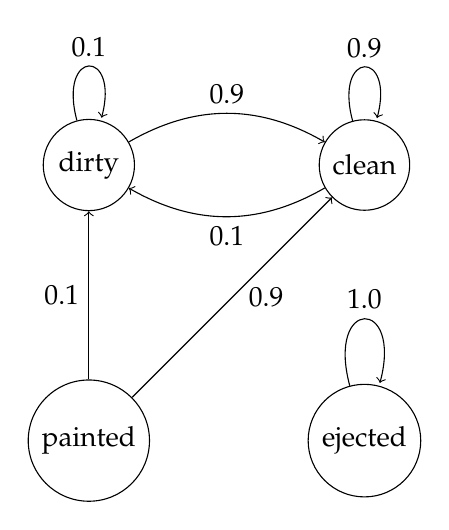
\begin{tikzpicture}[->]
      \node[state] (dirty) {dirty};
      \node[state, right of=dirty, xshift=2.5cm] (clean) {clean};
      \node[state, below of=dirty, yshift=-2.5cm] (painted) {painted};
      \node[state, below of=clean, yshift=-2.5cm] (ejected) {ejected};
      \draw (dirty) edge[loop above] node{0.1} (dirty)
      (dirty) edge[bend left, above] node{0.9} (clean)
      (clean) edge[loop above] node{0.9} (clean)
      (clean) edge[bend left, below] node{0.1} (dirty)
      (painted) edge[left] node{0.1} (dirty)
      (painted) edge[right] node{~0.9} (clean)
      (ejected) edge[loop above] node{1.0} (ejected);
    \end{tikzpicture}
  \end{center}

  You get reward +10 for ejecting a painted object, reward 0 for
  ejecting a non-painted object, reward 0 for any action on an "ejected"
  object, and reward -3 otherwise.  The MDP description would be
  completed by also specifying a discount factor.

\end{examplebox}



A {\it{policy}}\index{policy} is a function $\pi$
that specifies what action to take in each state.  The policy is what
we will want to learn; it is akin to the strategy that a player
employs to win a given game.  Below, we take just the initial steps
towards this eventual goal.  We describe how to evaluate how good a
policy is, first in the {\em finite horizon} case
(Section~\ref{sec-mdp_finite_horizon}) when the total number of
transition steps is finite.  In the finite horizon case, we typically denote
the policy as $\pi_h(s)$, where $h\in\mathbb N$ is a non-negative integer
denoting the number of steps remaining and $s \in \mathcal S$ is the current
state. Then we consider the {\em infinite horizon}
case (Section~\ref{sec-mdp_infinite_horizon}), when you
don't know when the game will be over.

% There are important algorithms that can be used to find good
% policies, under certain assumptions.  These will be discussed in
% Chapter~\ref{chap-reinforcement}.

%%%%%%%%%%%%%%%%%%%%%%%%%%%%%%%%%%%%%%%%
\subsection{Finite-horizon value functions}
\index{policy!finite horizon}
\label{sec-mdp_finite_horizon}

The goal of a policy is to maximize the expected total reward, averaged over
the stochastic transitions that the domain makes.  Let's first
consider the case where there is a finite {\em horizon} $H$,
indicating the total number of steps of interaction that the agent
will have with the {\sc mdp}\note{In the finite-horizon case, we usually
  set the discount factor $\gamma$ to 1.}.

We seek to measure the goodness of a
policy. We do so by defining for a given horizon $h$ and {\sc mdp} policy $\pi_h$, 
the ``horizon $h$ {\em value}'' of a state, $V^{h}_\pi(s)$.  We
do this by induction on the horizon, which is the {\em number of steps
    left to go}.

The base case is when there are no steps remaining, in which case, no
matter what state we're in, the value is 0,  so
\begin{equation}
  V^0_{\pi}(s) = 0\;\;.
  \label{eq:finite_val_0}
\end{equation}
Then, the value of a policy in state $s$ at horizon $h + 1$ is equal
to the reward it will get in state $s$ plus the next state's expected horizon $h$
value, discounted by a factor $\gamma$.  So, starting with horizons 1 and 2, and then
moving to the general case, we have:
\begin{align}
  V^1_{\pi}(s) & = R(s, \pi_1(s)) + 0                                                     \\
  \label{eq:finite_val_1}
  % V^2_{\pi}(s) & = R(s, \pi_2(s)) + \sum_{s'}T(s, \pi_2(s), s')  R(s', \pi(s'))      \\
  V^2_{\pi}(s) & = R(s, \pi_2(s)) +  \gamma \sum_{s'}T(s, \pi_2(s), s')  V^1_{\pi}(s')      \\
  \vdots
  \nonumber                                                                             \\
  V^h_{\pi}(s) & = R(s, \pi_h(s)) + \gamma \sum_{s'}T(s, \pi_h(s), s')  V^{h - 1}_{\pi}(s')
  \label{eq:finite_value}
\end{align}
The sum over $s'$ is an {\em expectation}\index{expectation}: it
considers all possible next states $s'$, and computes an average of
their $(h-1)$-horizon values, weighted by the probability that the
transition function from state $s$ with the action chosen by the
policy $\pi_h(s)$ assigns to arriving in state $s'$, and discounted by $\gamma$.

\question{What is $\sum_{s'} T(s, a, s')$ for any particular $s$ and $a$?}

\question{Convince yourself that Eqs.~\ref{eq:finite_val_0}
  and~\ref{eq:finite_val_1} are special cases of Eq.~\ref{eq:finite_value}.}

Then we can say that a policy $\pi$ is better than policy $\bar{\pi}$ for horizon
$h$ if and only if for all $s \in \mathcal S$,
$V_{\pi}^h(s) \geq V_{\bar{\pi}}^h(s)$ and there exists at least one $s
  \in \mathcal S$ such that $V_{\pi}^h(s) > V_{\bar{\pi}}^h(s)$.

%%%%%%%%%%%%%%%%%%%%%%%%%%%%%%%%%%%%%%%%
\subsection{Infinite-horizon value functions}
\label{sec-mdp_infinite_horizon}
\label{sec-discount}
\index{policy!infinite horizon}

More typically, the actual finite horizon is not known, i.e., when you
don't know when the game will be over!  This is called the {\em
    infinite horizon} version of the problem.  How does one evaluate the
goodness of a policy in the infinite horizon case?

If we tried to simply take our definitions above and use them for an
infinite horizon, we could get in trouble. Imagine we get a reward of
1 at each step under one policy and a reward of 2 at each step under a
different policy. Then the reward as the number of steps grows in each
case keeps growing to become infinite in the limit of more and more
steps. Even though it seems intuitive that the second policy should
be better, we can't justify that by saying $\infty < \infty$.

One standard approach to deal with this problem is to consider the
\emph{discounted} infinite horizon\index{policy!infinite horizon!discount factor}.
We will generalize from the finite-horizon case by adding a discount factor.

In the finite-horizon case, we valued a
policy based on an expected finite-horizon value:
\begin{equation}
  \mathbb{E}\left[\sum_{t = 0}^{h-1} \gamma^t R_t \mid \pi, s_0\right]\;\;,
  \label{eq:exp_finite}
\end{equation}
where $R_t$ is the reward received at time $t$.

\begin{examplebox}
  What is $\mathbb{E}\left[ \cdot \right ]$?  This mathematical
  notation indicates an {\em expectation}, i.e., an average
  taken over all the random possibilities which may occur for the
  argument.  Here, the expectation is taken over the {\em conditional
      probability} $Pr(R_t = r \mid \pi, s_0)$, where $R_t$ is the random
  variable for the reward, subject to the policy being $\pi$ and the
  state being $s_0$. Since $\pi$ is a function, this notation is
  shorthand for conditioning on all of the random variables implied by
  policy $\pi$ and the stochastic transitions of the MDP.

  \bigskip
  A very important point is that $R(s,a)$ is always deterministic (in this class) for
  any given $s$ and $a$. Here $R_t$ represents the set of all possible
  $R(s_t,a)$ at time step $t$; this $R_t$ is a random variable because
  the state we're in at step $t$ is itself a random variable, due to prior
  stochastic state transitions up to but not including at step $t$ and prior
  (deterministic) actions dictated by policy $\pi.$
\end{examplebox}

Now, for the infinite-horizon case, we select a discount factor $0 \leq \gamma \leq 1$,
and evaluate a policy based on its expected {\it{infinite horizon discounted value}}:
\begin{equation}
  \mathbb{E}\left[\sum_{t = 0}^{\infty}\gamma^tR_t \mid \pi, s_0\right]
  = \mathbb{E}\left[R_0  + \gamma R_1 + \gamma^2 R_2 + \ldots \mid \pi,  s_0\right] \;\;.
  \label{eq:exp_infinite}
\end{equation}
Note that the $t$ indices here are not the number of steps to go, but
actually the number of steps forward from the starting state (there is
no sensible notion  of ``steps to go'' in the infinite horizon case).

\begin{examplebox}
  Eqs.~\ref{eq:exp_finite} and~\ref{eq:exp_infinite} are a conceptual
  stepping stone. Our main objective is to get to
  Eq.~\ref{eq:inifite_horiz_value}, which can also be viewed
  as including $\gamma$ in Eq.~\ref{eq:finite_value}, with
  the appropriate definition of the infinite-horizon value.
\end{examplebox}

There are two good intuitive motivations for discounting.  One is
related to economic theory and the present value of money: you'd
generally rather have some money today than that same amount of money
next week (because you could use it now or invest it).  The other is
to think of the whole process terminating, with probability $1-\gamma$
on each step of the interaction\note{At every
  step, your expected future lifetime, given that you have survived
  until now, is $1 / (1 - \gamma)$.}.  This value is the expected amount of
reward the agent would gain under this terminating model.

\question{Verify this fact: if, on every day you wake up, there is a
  probability of $1 - \gamma$ that today will be your last day, then
  your expected lifetime is $1 / (1 - \gamma)$ days.  }

Let us now evaluate a policy in terms of the expected discounted
infinite-horizon value that the agent will get in the {\sc mdp} if it
executes that policy.  We define the infinite-horizon value of a state
$s$ under policy $\pi$ as
\begin{equation}
  V_{\pi}(s) = \mathbb{E}[R_0 + \gamma R_1 + \gamma^2 R_2 +
    \dots \mid \pi, S_0 = s] = \mathbb{E}[R_0 + \gamma(R_1 + \gamma(R_2 + \gamma
    \dots))) \mid \pi, S_0 = s] \;\;.
\end{equation}
Because the expectation of a linear combination of random variables is
the linear combination of the expectations, we have
\begin{align}
  V_{\pi}(s) & = \mathbb{E}[R_0 \mid \pi, S_0 = s] + \gamma  \mathbb{E}[
    R_1 + \gamma(R_2 + \gamma \dots))) \mid \pi, S_0 = s]
  \nonumber
  \\
             & = R(s, \pi(s)) + \gamma\sum_{s'}T(s, \pi(s), s')V_{\pi}(s') \; .
  \label{eq:inifite_horiz_value}
\end{align}\note{This is {\em so} cool!  In a discounted model, if you find that
  you survived this round and landed in some state $s'$, then you have
  the same expected future lifetime as you did before.  So the value
  function\index{value function} that is relevant in that state is
  exactly the same one as in state $s$.}

The equation defined in Eq.~\ref{eq:inifite_horiz_value} is known as the Bellman Equation,
which breaks down the value function into the immediate reward and the (discounted) future
value function.
You could write down one of these equations for each of the $n =
  |\mathcal S|$ states. There are $n$ unknowns $V_{\pi}(s)$.  These are
linear equations, and standard software (e.g., using Gaussian
elimination or other linear algebraic methods) will, in most cases,
enable us to find the value of each state under this policy.

%%%%%%%%%%%%%%%%%%%%%%%%%%%%%%%%%%%%%%%%%%%%%%%%%%%%%%%%%%%%%%%%%%%%%%%%%%%%%
\section{Finding policies for MDPs}

\label{sec-finding_mdp_policies}

Given an {\sc mdp}, our goal is typically to find a policy that is
optimal in the sense that it gets as much total reward as possible, in
expectation over the stochastic transitions that the domain makes.  We
build on what we have learned about evaluating the goodness of a
policy (Sections~\ref{sec-mdp_finite_horizon}
and~\ref{sec-mdp_infinite_horizon}), and find optimal policies for the
finite horizon case (Section~\ref{sec-mdp_finite_horizon_optimal}),
then the infinite horizon case
(Section~\ref{sec-mdp_infinite_horizon_optimal}).

%%%%%%%%%%%%%%%%%%%%%%%%%%%%%%%%%%%%%%%%
\subsection{Finding optimal finite-horizon policies}

\label{sec-mdp_finite_horizon_optimal}

How can we go about finding an optimal policy for an {\sc mdp}?
\index{policy!optimal policy} We could imagine enumerating all
possible policies and calculating their value functions\index{value
  function!calculating value function} as in the previous section and
picking the best one -- but that's too much work!

The first observation to make is that, in a finite-horizon problem,
the best action to take depends on the current state, but also on the
horizon: imagine that you are in a situation where you could reach a
state with reward 5 in one step or a state with reward 100 in two
steps.  If you have at least two steps to go, then you'd move toward
the reward 100 state, but if you only have one step left to go, you should
go in the direction that will allow you to gain 5!

One way to find an optimal policy is to compute an optimal {\em action-value function}, $Q$\index{Q-function}\index{optimal
  action-value function}.  For the finite-horizon case, we define
$Q^h(s, a)$ to be the expected value of
\begin{itemize}
  \item starting in state $s$,
  \item executing action $a$, and
  \item continuing for $h - 1$ more steps executing an optimal policy
        for the appropriate horizon on each step.
\end{itemize}
Similar to our definition of $V^h$ for evaluating a policy, we define
the $Q^h$ function recursively according to the horizon.  The only
difference is that, on each step with horizon $h$, rather than
selecting an action specified by a given  policy, we select the value
of $a$ that will maximize the expected $Q^h$ value of the next state.
\begin{align}
  Q^0(s, a) & = 0                                                                 \\
  Q^1(s, a) & = R(s, a) + 0                                                       \\
  % Q^2(s, a) & = R(s, a) + \sum_{s'}T(s, a, s') \max_{a'} R(s', a')         \\
  Q^2(s, a) & = R(s, a) + \gamma \sum_{s'}T(s, a, s') \max_{a'} Q^1(s', a')       \\
  \vdots
  \nonumber                                                                       \\
  Q^h(s, a) & = R(s, a) + \gamma \sum_{s'}T(s, a, s') \max_{a'} Q^{h - 1}(s', a')
\end{align}
where $(s',a')$ denotes the next time-step state/action pair. We can solve for the values of $Q^h$ with a simple recursive algorithm
called {\it{finite-horizon value iteration}} that just computes $Q^h$ starting
from horizon 0 and working backward to the desired horizon
$H$. Given $Q^h$, an optimal $\pi_h^*$ can be found as follows:
\begin{equation}
  \pi_h^*(s) = \arg\max_{a}Q^h(s, a) \;\;.
\end{equation}
which gives the \emph{immediate} best action(s) to take when there are $h$ steps left; then $\pi_{h-1}^*(s)$ gives the best action(s) when there are $(h-1)$ steps left, and so on. In the case where there are multiple best actions, we typically can break ties randomly.


Additionally, it is worth noting that in order for such an optimal policy to be
computed, we assume that the reward function $R(s,a)$ is bounded on the set of
all possible (state, action) pairs. Furthermore, we will assume that the set of
all possible actions is finite.
\question{The optimal value function is unique, but the optimal policy
  is not.  Think of a situation in which there is more than one
  optimal policy.}

\begin{examplebox} {\bf Dynamic programming}
  (somewhat counter-intuitively, dynamic programming is neither really
  ``dynamic'' nor a type of ``programming'' as we typically understand
  it) is a technique for designing efficient algorithms.  Most methods
  for solving MDPs or computing value functions rely on dynamic
  programming to be efficient.  The {\em principle of dynamic
      programming}\index{dynamic programming} is to compute and store
  the solutions to simple sub-problems that can be re-used later in
  the computation.  It is a very important tool in our algorithmic
  toolbox.

  Let's consider what would happen if we tried to compute $Q^4(s,
    a)$ for all $(s, a)$ by directly using the definition:
  \begin{itemize}
    \item To compute $Q^4(s_i, a_j)$ for any one $(s_i, a_j)$, we would
          need to compute $Q^3(s, a)$ for all $(s, a)$
          pairs.
    \item To compute $Q^3(s_i, a_j)$ for any one $(s_i, a_j)$, we'd need to
          compute $Q^2(s, a)$ for all $(s, a)$ pairs.
    \item To compute $Q^2(s_i, a_j)$ for any one $(s_i, a_j)$, we'd
          need to compute $Q^1(s, a)$ for all $(s, a)$ pairs.
    \item Luckily, those are just our $R(s, a)$ values.
  \end{itemize}

  So, if we have $n$ states and $m$ actions, this is $O((mn)^3)$
  work --- that seems like way too much, especially as the horizon
  increases!  But observe that we really only have $mnh$ values that
  need to be computed: $Q^h(s, a)$ for all $h, s, a$.  If we start with
  $h=1$, compute and store those values, then using and reusing the
  $Q^{h-1}(s, a)$ values to compute the $Q^h(s, a)$ values, we can do
  all this computation in time $O(mnh)$, which is much better!

\end{examplebox}

%%%%%%%%%%%%%%%%%%%%%%%%%%%%%%%%%%%%%%%%
\subsection{Finding optimal infinite-horizon policies}
\label{sec-mdp_infinite_horizon_optimal}

In contrast to the finite-horizon case, the best way of behaving in an
infinite-horizon discounted {\sc mdp} is not time-dependent. That is,
the decisions you make at time $t = 0$ looking forward to infinity,
will be the same decisions that you make at time $t = T$ for any positive
$T$, also looking forward to infinity.

An important theorem about {\sc mdp}s is: in the infinite-horizon
case, there exists a stationary\index{policy!stationary policy}
\note{Stationary means that it doesn't change over time; in contrast,
the optimal policy in a finite-horizon {\sc mdp} is {\em
    non-stationary.}} optimal policy $\pi^*$ (there may be more than
one) such that for all $s \in \mathcal S$ and all other policies
$\pi$, we have
\begin{equation}
  V_{\pi^*}(s) \ge V_{\pi}(s) \;\;.
\end{equation}

% Let $n = |\mathcal S|$ andd $m = |\mathcal A|$. Algorithm for finding $\pi^*$:
% \begin{itemize}
% \item
% enumerate and test, complexity is $O(m^n)$
% \item
% linear programming, complexity is $O(\text{poly}(n, m b))$ where $b$ is the number of bits per element of $T, R$
% \item
% policy iteration, complexity is $O(\text{poly}(n, m, \text{bits}(\gamma)))$, requires solving lots of $n \times n$ systems
% \item
% {\underline{value iteration}}, complexity is $O\left(\text{poly}(n, m, b, \frac{1}{1 - \gamma}\right)$
% \end{itemize}
% The latter is easy to implement and the foundation for many reinforcement-learning methods.

There are many methods for finding an optimal policy for an {\sc mdp}.
We have already seen the finite-horizon value iteration case.  Here we
will study a very popular and useful method for the infinite-horizon
case, {\em infinite-horizon value iteration}.  It is also important to
us, because it is the basis of many {\em reinforcement-learning} methods.

We will again assume that the reward function $R(s,a)$ is bounded on the
set of all possible (state, action) pairs and additionally that the number
of actions in the action space is finite.
Define $Q(s, a)$ to be the expected infinite-horizon discounted
value of being in state $s$, executing action $a$, and executing
an optimal policy $\pi^*$ thereafter. Using similar reasoning to the
recursive definition of $V_\pi,$ we can express this value
recursively as
\begin{equation}
  Q(s, a) = R(s, a) + \gamma\sum_{s'}T(s, a, s')\max_{a'}Q(s',
  a') \;\;.
\end{equation}

This is also a set of equations, one for each $(s, a)$ pair.  This
time, though, they are not linear (due to the $\max$ operation), and so
they are not easy to solve.  But there is a theorem that says they
have a unique solution!

Once we know the optimal action-value function, then we can extract an
optimal policy $\pi^*$ as
\begin{equation}
  \pi^*(s) = \arg\max_{a}Q(s, a) \;\;.
\end{equation}
\note{As in the finite-horizon case, there may be more than one optimal
  policy in the infinite-horizon case.}

We can iteratively solve for the $Q^*$ values with the
infinite-horizon value iteration algorithm, shown below:

\begin{codebox}
  \Procname{$\proc{Infinite-Horizon-Value-Iteration}(\mathcal S, \mathcal A, T, R, \gamma, \epsilon)$}
  \li     \For $s \in \mathcal{S}, a \in \mathcal{A}:$
  \Do
  \li        $Q_{\text{old}}(s, a) = 0$
  \End
  \li     \While not converged:
  \Do
  \li        \For $s \in \mathcal{S}, a \in \mathcal{A}:$
  \Do
  \li           $Q_{\text{new}}(s, a) = R(s, a) + \gamma\sum_{s'}T(s, a, s')\max_{a'}Q_{\text{old}}(s', a')$
  \End

  \li      \If $\max_{s, a}\lvert Q_{\text{old}}(s, a) - Q_{\text{new}}(s, a)\rvert < \epsilon:$
  \Do
  \li           return $Q_{\text{new}}$
  \End
  \li      $Q_{\text{old}} = Q_{\text{new}}$
  \End
\end{codebox}

\paragraph*{Theory}

There are a lot of nice theoretical results about infinite-horizon value iteration.
For some given (not necessarily optimal) $Q$ function, define
$\pi_{Q}(s) = \arg\max_{a}Q(s, a)$.
\begin{itemize}
  \item After executing infinite-horizon value
        iteration with convergence hyper-parameter $\epsilon$,
        \note{Note the new
          notation!  Given two functions $f$ and $f'$, we
          write $\lVert f - f' \rVert_\text{max}$ to mean $\max_x \lvert f(x)
            - f'(x)\rvert$.   It measures the maximum absolute
          disagreement between the two functions at any input $x$.}
        \begin{equation}
          \lVert  V_{\pi_{Q_{\text{new}}}} - V_{\pi^*} \rVert_{\text{max}} < \epsilon \;\; .
        \end{equation}
        %
  \item
        There is a value of $\epsilon$ such that
        \begin{equation}
          \Vert Q_{\text{old}} - Q_{\text{new}} \rVert_{\text{max}} <
          \epsilon \Longrightarrow \pi_{Q_{\text{new}}} = \pi^*
        \end{equation}
  \item  As the algorithm executes,
        $\lVert V_{\pi_{Q_{\text{new}}}} - V_{\pi^*} \Vert_{\text{max}}$ decreases
        monotonically on each iteration.
  \item The algorithm  can be executed asynchronously, in parallel: as
        long as all $(s, a)$ pairs are updated infinitely often in an
        infinite run, it still converges to the optimal value.
        \note{This is very important for reinforcement learning.}

\end{itemize}

%%% Local Variables:
%%% mode: latex
%%% TeX-master: "top"
%%% End:

\chapter{Reinforcement learning}
\label{chap-reinforcement}

So far, all the learning problems we have looked at have been {\em supervised}, that is, for each training input $\ex{x}{i}$, we
are told which value $\ex{y}{i}$ should be the output. {\em Reinforcement learning}\index{reinforcement learning} differs from previous learning problems in several important ways:

% \note{We also looked at Markov Decision Processes; but in that setting, we do not \emph{learn} anything based on any data. Instead, the whole process is fully defined.}

\begin{itemize}
  \item The learner interacts explicitly with an environment, rather
        than implicitly (as in supervised learning) through an available
        training data set of $(\ex{x}{i}, \ex{y}{i})$ pairs drawn from the
        environment.
  \item The learner has some choice over what new information it
        seeks to gain from the environment.
  \item The learner updates models incrementally \note{{\em Online
              learning} is a variant of supervised learning in which new data
          pairs become available over time and the model is updated, e.g., by
          retraining over the entire larger data set, or by weight update
          using just the new data.} as additional information about the
        environment becomes available.
\end{itemize}

In a reinforcement learning problem, the interaction with the
environment takes a particular form:
\begin{center}
  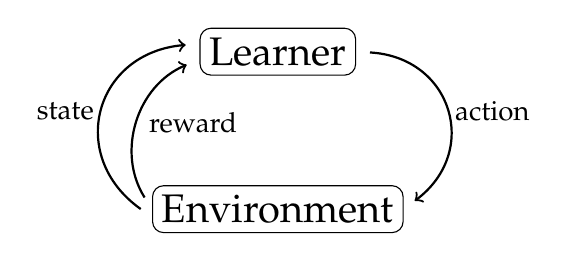
\begin{tikzpicture}[main node/.style={draw,rounded corners,font=\Large},
      arr/.style={->, thick, shorten <=5pt, shorten >=5pt,}]
    \node[main node] (rl) at (0,1) {Learner};
    \node[main node] (env) at (0,-1) {Environment};
    \draw (env.west) edge[arr, bend left=50, looseness=1.1]
    node[right] {reward} ($(rl.west) + (0, -0.1)$);
    \draw ($(env.west) + (0,-0.1)$) edge[arr, bend left=70, looseness=1.5]
    node[left] {state} ($(rl.west) + (0, 0.1)$);
    \draw (rl.east) edge[arr, bend left=70, looseness=1.5]
    node[right] {action} (env.east);
  \end{tikzpicture}
\end{center}
\begin{compactitem}
  \item Learner observes {\em input} state $\ex{s}{i}$
  \item Learner generates {\em output} action $\ex{a}{i}$
  \item Learner observes {\em reward} $\ex{r}{i}$
  \item Learner observes {\em input} state $\ex{s}{i+1}$
  \item Learner generates {\em output} action $\ex{a}{i+1}$
  \item Learner observes {\em reward} $\ex{r}{i+1}$
  \item $\ldots$
\end{compactitem}
Similar to MDPs, the learner is supposed to find a {\em policy}\index{reinforcement
  learning!policy}\index{policy!reinforcement learning}, mapping a state $s$
to action $a$, that maximizes expected reward over time.

%% \question{Suppose you have the entire history of $(\ex{s}{i},
%%   \ex{a}{i}, \ex{r}{i})$ tuples from previous interactions with
%%   the environment. Could you use supervised learning to build a model
%%   that takes input (state) $s$ and predicts output (preferred action)
%%   $a$? What assumptions might be needed?}


% This problem setting is equivalent to {\em online} supervised
% learning under the following assumptions:
% \begin{enumerate}
%   \item The space of possible outputs is binary
%         (e.g., $\{+1, -1\}$) and the space of possible rewards is binary
%         (e.g., $\{+1, -1\}$);
%   \item $\ex{s}{i}$ is independent of all previous $\ex{s}{j}$ and
%         $\ex{a}{j}$; and
%   \item $\ex{r}{i}$ depends only on $\ex{s}{i}$ and $\ex{a}{i}$.
% \end{enumerate}
% In this
% case, for any experience tuple $(\ex{s}{i}, \ex{a}{i}, \ex{r}{i})$, we
% can generate a supervised training example, which is equal to
% $(\ex{s}{i}, \ex{a}{i})$ if $\ex{r}{i} = +1$ and $(\ex{s}{i},
%   -\ex{a}{i})$ otherwise.
% \question{What supervised-learning loss function would this objective
%   correspond to?}

% Markov decision processes ({\sc mdp}s) form a more general and
% flexible basis for reinforcement learning.  We began in
% Section~\ref{sec-finding_mdp_policies} with a discussion of how to
% find optimal policies for {\sc mdp}s when the {\sc mdp} is completely
% known in advance.  However, in many scenarios, full information about
% the {\sc mdp} is unavailable.  For example, consider the case when the
% above three assumptions do not hold.  When we relax assumption 1
% above, we have the class of {\em bandit problems}\index{bandit
%   problem}, which we discuss in Section~\ref{sec-bandit}.  If we relax
% assumption 2, but assume that the environment that the agent is
% interacting with is an {\sc mdp}, so that $\ex{s}{i}$ depends only on
% $\ex{s}{i-1}$ and $\ex{a}{i-1}$ then we are in the classical {\em
%     reinforcement-learning} setting, which we discuss in
% Section~\ref{rl}.  Weakening the assumptions further, for instance,
% not allowing the learner to observe the current state completely and
% correctly, makes the problem into a {\em partially observed
%     MDP}\index{Markov decision policy!partially observed MDP} ({\sc
%   pomdp}), which is substantially more difficult, and beyond the scope
% of this class.


\section{Reinforcement learning algorithms overview}
\label{rl}

A {\em reinforcement learning ({\sc rl})
    algorithm}\index{reinforcement learning!RL algorithm} is a kind of a
policy that depends on the whole history of states, actions, and
rewards and selects the next action to take. There are several
different ways to measure the quality of an {\sc rl} algorithm,
including:
\begin{itemize}
  \item Ignoring the $r^{(i)}$ values that it gets {\em while} learning,
        but considering how many interactions with the environment are
        required for it to learn a policy $\pi: \mathcal{S} \rightarrow
          \mathcal{A}$ that is nearly optimal.
  \item Maximizing the expected sum of discounted rewards while
        it is learning.
\end{itemize}
Most of the focus is on the first criterion (which is called ``sample efficiency''), because the second one is
very difficult.  The first criterion is reasonable when the learning
can take place somewhere safe (imagine a robot learning, inside the
robot factory, where it can't hurt itself too badly) or in a simulated
environment.

Approaches to reinforcement learning differ significantly according to
what kind of hypothesis or model is being learned. Roughly speaking, RL
methods can be categorized into model-free methods and model-based
methods. 
The main distinction is that model-based methods explicitly
learn the transition and reward models to assist the end-goal of
learning a policy; model-free methods do not.  We will start our discussion with the model-free
methods, and introduce two of the arguably most popular types of algorithms,
Q-learning (Section~\ref{sec-q_learning}) and policy gradient
(Section~\ref{sec-rl_policy_search}).  We then describe
model-based methods (Section~\ref{sec-rl_model_based}). Finally, we
briefly consider ``bandit'' problems (Section~\ref{sec-bandit}), which differ
from our {\sc mdp} learning context by having probabilistic rewards.




%%%%%%%%%%%%%%%%%%%%
\section{Model-free methods}

Model-free methods are methods that do not explicitly learn transition
and rewards models. Depending on what is explicitly being learned,
model-free methods are sometimes further categorized into value-based
methods (where the goal is to learn/estimate a value function)
% (where value is a shorthand for value functions) 
and
policy-based methods (where the goal is to directly learn an optimal policy). It's important to note that such
categorization is approximate and the boundaries are blurry. In fact,
current RL research tends to combine the learning of value functions,
policies, and transition and reward models all into a complex learning
algorithm, in an attempt to combine the strengths of each approach.


% --e.g., in (tabular) Q-learning (Section \ref{sec-q_learning}) right
% below, the Machine Learning model used is a table. We will soon see
% other (ML) models used in the model-free methods, such as neural
% networks.


\subsection{Q-learning}\label{sec-q_learning}
Q-learning is a frequently used class of RL algorithms that
concentrates on learning (estimating) the state-action value function, i.e.,
the $Q$ function. Specifically, recall the {\sc mdp} value-iteration update:
\note{The thing that most students seem to get confused about is when
  we do value iteration and when we do Q learning.  Value iteration
  assumes you know $T$ and $R$ and just need to {\em compute} $Q$.  In
  $Q$ learning, we don't know or even directly estimate $T$ and $R$:
  we estimate $Q$ directly from experience!}
\begin{equation}
  Q(s,a) = R(s,a) + \gamma \sum_{s'} T(s,a,s')\max_{a'}Q(s',a')
\end{equation}
The Q-learning algorithm below adapts this value-iteration idea to the
  {\sc rl} scenario, where we do not know the transition function $T$ or
reward function $R$, and instead rely on samples to perform the updates.
\begin{codebox}
  \Procname{$\proc{Q-Learning}(\mathcal{S}, \mathcal{A},  \gamma, \epsilon, \alpha, s_0)$}\label{proc:Q_learn}
  \li \For $s \in \mathcal{S}, a \in \mathcal{A}:$
  \li   \Do
  ${Q_{old}}(s, a) = 0$
  \End
  \li $s \gets s_0$
  \li \While True:
  \li   \Do
  $a \gets \text{select}\_\text{action}(s, {Q_{old}}(s, a))$
  \li     $r,s' \gets \text{execute}(a)$
  \li     ${Q}_{\text{new}}(s, a) = (1-\alpha){Q}_{\text{old}}(s, a)
    + \alpha(r + \gamma \max_{a'}{Q}_{\text{old}}(s', a'))$
  \li $s \gets s'$
  \li      \If $\max_{s, a}\lvert Q_{\text{old}}(s, a) - Q_{\text{new}}(s, a)\rvert < \epsilon:$
  \Do
  \li           return $Q_{\text{new}}$
  \End
  \li      $Q_{\text{old}} = Q_{\text{new}}$
  \End
\end{codebox}

With the pseudo-code provided for \nameref{proc:Q_learn}, there are a few
key things to note. First, we must determine which state to initialize the
learning from. In the context of a game, this initial state may be well defined.
In the context of a robot navigating an environment, one may consider
sampling the initial state at random. In any case, the initial state is necessary
to determine the trajectory the agent will experience as it navigates the environment.
Second, different contexts will influence how we want to choose when to stop
iterating through the while loop. Again, in some games there may be a clear
terminating state based on the rules of how it is played. On the other hand,
a robot may be allowed to explore an environment \emph{ad infinitum}.
In such a case, one may consider either setting a fixed number of transitions to take
or we may want to stop iterating once the values in the Q-table are not changing.
Finally, a single trajectory through the environment may not be sufficient to adequately
explore all state-action pairs. In these instances, it becomes necessary to run
through a number of iterations of the \nameref{proc:Q_learn} algorithm, potentially
with different choices of initial state $s_0$\note{This notion of running a number
  of instances of \nameref{proc:Q_learn} is often referred to as experiencing multiple
  \emph{episodes}.}. Of course, we would then want to modify \nameref{proc:Q_learn} such
that the Q table is not reset with each call.

Now, let's dig in to what is happening in \nameref{proc:Q_learn}.
Here, $\alpha\in (0,1]$ represents the ``learning rate,'' which needs to decay
for convergence purposes, but in practice is often set to a
constant. It's also worth mentioning that Q-learning assumes a
discrete state and action space where states and actions take on
discrete values like $1,2,3,\dots$ etc. In contrast, a continuous
state space would allow the state to take values from, say, a
continuous range of numbers; for example, the state could be any real
number in the interval $[1,3]$. Similarly, a continuous action space
would allow the action to be drawn from, e.g., a continuous range of
numbers. There are now many extensions developed based on Q-learning
that can handle continuous state and action spaces (we'll look at one
soon), and therefore the algorithm above is also sometimes referred to
more 
% verbosely or 
specifically as tabular Q-learning.

In the Q-learning update rule
\begin{equation}\label{q_avg}
  Q[s, a] \leftarrow (1-\alpha)Q[s, a]
  + \alpha(r + \gamma \max_{a'}Q[s',a'])
\end{equation}
the term $r + \gamma \max_{a'} Q[s',a']$ is often referred to as the
(one-step look-ahead) \emph{target}. The update can be viewed as a
combination of two different iterative processes that we have already
seen: the combination of an old estimate with the target using a
running average with a learning rate $\alpha$, and the
dynamic-programming update of a $Q$ value from value iteration.


Eq.~\ref{q_avg} can also be equivalently rewritten as
\begin{equation}\label{td:q}
  Q[s, a] \leftarrow Q[s, a]
  + \alpha\left((r + \gamma \max_{a'}
  Q[s',a'])-Q[s,a]\right),
\end{equation}
which allows us to interpret Q-learning in yet another way: we make an
update (or correction) based on the temporal difference between the
target and the current estimated value $Q[s, a].$


% It is actually not a gradient update, but later, when we consider
% function approximation, we will treat it as if it were.}

% And besides an "almost" gradient interpretation, writing the
% Q-learning update rule in (\ref{td:q}) form also allows us to make
% a connection to a whole family of sampling-based reinforcement
% learning methods called {\em temporal difference} (TD) learning
% method\index{reinforcement learning!temporal difference method}. TD
% methods are so-named


The Q-learning algorithm above includes a procedure called {\it select\_action},
that, given the current state $s$ and current $Q$ function, has to decide
which action to take.  If the $Q$ value is estimated very accurately
and the agent is behaving in the world, then generally we would want
to choose the apparently optimal action $\argmax{a \in \mathcal{A}}
  Q(s,a)$.  But, during learning, the $Q$ value estimates won't be very
good and exploration is important.  However, exploring completely at
random is also usually not the best strategy while learning, because
it is good to focus your attention on the parts of the state space
that are likely to be visited when executing a good policy (not a bad
or random one).

A typical action-selection strategy that attempts to address this
  {\em exploration versus exploitation} dilemma is the so-called {\em
$\epsilon$-greedy} strategy:
\begin{itemize}
  \item with probability $1-\epsilon$, choose
        $\argmax{a \in \mathcal{A}} Q(s,a)$;
  \item with probability $\epsilon$, choose the action $a \in \mathcal{A}$
        uniformly at random.
\end{itemize}
where the $\epsilon$ probability of choosing a random action helps the
agent to explore and try out actions that might not seem so desirable
at the moment.


Q-learning has the surprising property that it is {\em guaranteed} to
converge to the actual optimal $Q$ function under fairly weak
conditions!  Any exploration strategy is okay as long as it tries
every action infinitely often on an infinite run (so that it doesn't
converge prematurely to a bad action choice).

Q-learning can be very inefficient. Imagine a robot that has a
choice between moving to the left and getting a reward of 1, then
returning to its initial state, or moving to the right and walking
down a 10-step hallway in order to get a reward of 1000, then
returning to its initial state.

\begin{center}
  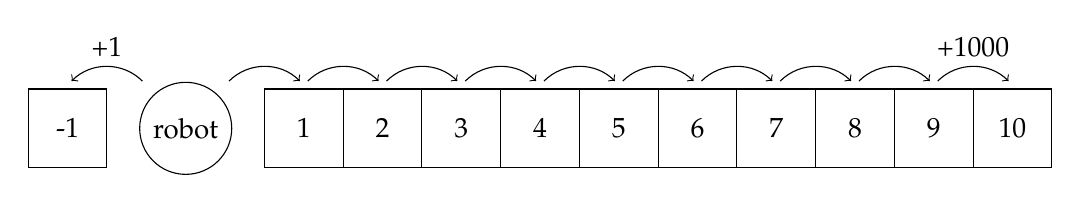
\begin{tikzpicture}
    \draw (-3,0) grid (-2,1);
    \draw (0,0) grid (10,1);
    \node[circle, draw] (robot) at (-1,.5) {robot};
    % right arrows
    \foreach \x in {1,2,3,4,5,6,7,8,9,10} {
        \coordinate (a) at (\x - 1.45, 1.1);
        \coordinate (b) at (\x - .55, 1.1);
        \draw (a) edge[->, bend left=45] coordinate (mid) (b);
        \node at (\x - .5, .5) {\x};
      }
    \node[above] (reward) at (mid) {+1000};

    % left arrow
    \coordinate (a) at (-2.45, 1.1);
    \coordinate (b) at (-1.55, 1.1);
    \draw (b) edge[->, bend right=45] node[above] {+1} (a);
    \node at (-2.5, .5) {-1};
  \end{tikzpicture}
\end{center}

The first time the robot moves to the right and goes down the hallway,
it will update the $Q$ value just for state 9 on the hallway and
action ``right'' to have a high value, but it won't yet understand
that moving to the right in the earlier steps was a good choice. The
next time it moves down the hallway it updates the value of the state
before the last one, and so on.  After 10 trips down the hallway, it
now can see that it is better to move to the right than to the left.

\setcounter{MaxMatrixCols}{20}

More concretely, consider the vector of Q values $Q(i = 0, \ldots, 9;
  \text{right})$, representing the Q values for moving right at each of
the positions $i = 0, \ldots, 9$. Position index $0$ is the starting
position of the robot as pictured above.

Then, for $\alpha=1$ and $\gamma = 0.9$, Eq.~\ref{td:q} becomes
\begin{equation}
  Q(i, \text{ right}) = R(i, \text{ right})
  + 0.9 \cdot \max_a Q(i+1, a).
\end{equation}
Starting with Q values of 0,
\begin{equation}
  Q^{(0)}(i = 0, \ldots, 9; \text{ right}) =
  \begin{bmatrix} 0 & 0 & 0 & 0 & 0 & 0 & 0 & 0 & 0 & 0 \end{bmatrix}.
\end{equation}
\note{We are violating our usual notational conventions here, and
  writing $\ex{Q}{i}$ to mean the Q value function that results after
  the robot runs all the way to the end of the hallway, when executing
  the policy that always moves to the right.}  Since the only nonzero
reward from moving right is $R(9, \text{ right}) = 1000$, after our
robot makes it down the hallway once, our new Q vector is
\begin{equation}
  Q^{(1)}(i = 0, \ldots, 9; \text{ right}) =
  \begin{bmatrix} 0 & 0 & 0 & 0 & 0 & 0 & 0 & 0 & 0 & 1000 \end{bmatrix}.
\end{equation}
After making its way down the hallway again,
$Q(8, \text{ right}) = 0 + 0.9 \cdot Q(9, \text{ right}) = 900$
updates:
\begin{equation}
  Q^{(2)}(i = 0, \ldots, 9; \text{ right}) =
  \begin{bmatrix}
    0 & 0 & 0 & 0 & 0 & 0 & 0 & 0 & 900 & 1000
  \end{bmatrix}.
\end{equation}
Similarly,
\begin{align}
  Q^{(3)}(i = 0, \ldots, 9; \text{ right})   & =
  \begin{bmatrix}
    0 & 0 & 0 & 0 & 0 & 0 & 0 & 810 & 900 & 1000
  \end{bmatrix}                 \\
  Q^{(4)}(i = 0, \ldots, 9; \text{ right})   & =
  \begin{bmatrix}
    0 & 0 & 0 & 0 & 0 & 0 & 729 & 810 & 900 & 1000
  \end{bmatrix}               \\
                                             & \vdotswithin{=} \\
  Q^{(10)}(i = 0, \ldots, 9;  \text{ right}) & =
  \begin{bmatrix}
    387.4 & 420.5 & 478.3 & 531.4 & 590.5 & 656.1 & 729 & 810
          & 900   & 1000
  \end{bmatrix},
\end{align}
and the robot finally sees the value of moving right from position 0.
\note{Here, we can see the exploration/exploitation dilemma in action: from the perspective of $s_0=0$, it
  will seem that getting the immediate reward of $1$
  is a better strategy without exploring the long hallway.}
\question{Determine the Q value functions that will result from updates due to the robot always executing the ``move left'' policy.}


\subsection{Function approximation: Deep Q learning}
In our Q-learning algorithm above, we essentially keep track of each
$Q$ value in a table, indexed by $s$ and $a$. What do we do if
$\mathcal{S}$ and/or $\mathcal{A}$ are large (or continuous)?

We can use a function approximator like a neural network to store Q
values. For example, we could design a neural network that takes in
inputs $s$ and $a$, and outputs $Q(s,a)$. We can treat this as a
regression problem, optimizing this loss\note{This is the so-called
  squared Bellman error; as the name suggests, it's closely related to
  the Bellman equation we saw in {\sc mdp}s in Chapter~\ref{chap-mdps}.
  Roughly speaking, this error measures how much the
  Bellman equality is violated.}:
\begin{equation}
  \left(Q(s,a) - (r + \gamma \max_{a'}Q(s',a'))\right)^2\;\;,
\end{equation}
where $Q(s, a)$ is now the output  of the neural network.

There are several different architectural choices for using a
neural network to approximate $Q$ values:
\begin{itemize}
  \item One network for each action $a$, that takes $s$ as input and
        produces $Q(s, a)$ as output;
  \item One single network that takes $s$ as input and produces a vector
        $Q(s, \cdot)$, consisting of the $Q$ values for each action; or
  \item One single network that takes $s, a$ concatenated into a vector
        (if $a$ is discrete, we would probably use a one-hot encoding,
        unless it had some useful internal structure) and produces $Q(s, a)$
        as output.
\end{itemize}

\note{For continuous action spaces, it is popular to use
  a class of methods called {\em actor-critic}
  methods\index{reinforcement!actor-critic methods}, which combine
  policy and value-function learning.  We won't get into them in
  detail here, though.}

The first two choices are only suitable for discrete (and not too big)
action sets.  The last choice can be applied for continuous actions,
but then it is difficult to find $\argmax{a \in \mathcal{A}} Q(s, a)$.

There are not many theoretical guarantees about Q-learning with
function approximation and, indeed, it can sometimes be fairly
unstable (learning to perform well for a while, and then getting
suddenly worse, for example).  But neural network Q-learning has also
had some significant successes.

One form of instability that we do know how to guard against is {\em
    catastrophic forgetting.}  In standard supervised learning, we
expect that the training $x$ values were drawn independently from some
distribution. \note{And, in fact, we routinely shuffle their order in
  the data file, anyway.}  But when a learning agent, such as a robot,
is moving through an environment, the sequence of states it encounters
will be temporally correlated. For example, the robot might spend 12
hours in a dark environment and then 12 in a light one.  This can mean
that while it is in the dark, the neural-network weight-updates will
make the $Q$ function ``forget'' the value function for when it's
light.

One way to handle this is to use $\emph{experience
    replay}$\index{experience replay}, where we save our $(s,a,s',r)$
experiences in a {\it replay buffer}.  Whenever we take a step in the
world, we add the $(s,a,s',r)$ to the replay buffer and use it to do a
Q-learning update.  Then we also randomly select some number of tuples
from the replay buffer, and do Q-learning updates based on them, as
well.  In general it may help to keep a {\em sliding
    window}\index{sliding window} of just the 1000 most recent
experiences in the replay buffer.  (A larger buffer will be necessary
for situations when the optimal policy might visit a large part of the
state space, but we like to keep the buffer size small for memory
reasons and also so that we don't focus on parts of the state space
that are irrelevant for the optimal policy.)  The idea is that it will
help us propagate reward values through our state space more
efficiently if we do these updates. We can see it as doing something
like value iteration, but using samples of experience rather than a
known model.

\subsection{Fitted Q-learning}
An alternative strategy for learning the $Q$ function that is somewhat
more robust than the standard $Q$-learning algorithm is a method
called {\em fitted Q}.\index{fitted Q-learning}

\begin{codebox}
  \Procname{$\proc{Fitted-Q-Learning}(\mathcal{A}, s_0, \gamma, \alpha,
      \epsilon, m)$}
  \li $s \gets s_0$ \Comment (e.g., $s_0$ can be drawn randomly from $\mathcal{S}$)
  \li $\mathcal{D} = \{\;\}$
  \li initialize neural-network representation of $Q$
  \li \While True: \Do
  \li  $\mathcal{D}_\text{new}$ = experience from executing $\epsilon$-greedy policy based
  on $Q$ for $m$ steps
  \li $\mathcal{D} = \mathcal{D} \cup \mathcal{D}_\text{new}$ represented
  as $(s, a, s', r)$ tuples
  \li $\mathcal{D}_\text{supervised} = \{(\ex{x}{i}, \ex{y}{i})\}$  where $\ex{x}{i} =
    (s, a)$ and $\ex{y}{i} = r + \gamma \max_{a' \in \mathcal{A}} Q(s', a')$
  \li \;\;\;for each tuple $\ex{(s, a, s', r)}{i} \in \mathcal{D}$
  \li re-initialize neural-network representation of $Q$
  \li $Q = \proc{supervised-NN-regression}(\mathcal{D}_\text{supervised})$
  \End
\end{codebox}

Here, we alternate between using the policy induced by the current $Q$
function to gather a batch of data $\mathcal{D}_\text{new}$, adding it
to our overall data set $\mathcal{D}$, and then using supervised
neural-network training to learn a representation of the $Q$ value
function on the whole data set.  This method does not mix the
dynamic-programming phase (computing new $Q$ values based on old ones)
with the function approximation phase (supervised training of the
neural network) and avoids catastrophic forgetting.  The regression
training in line 9 typically uses squared error as a loss function and
would be trained until the fit is good (possibly measured on held-out
data).


%%%%%%%%%%%%%%%%%%%%


\subsection{Policy gradient}
\label{sec-rl_policy_search}

A different model-free strategy is to search directly for a good
policy.  The strategy here is to define a functional form $f(s;\theta)
  = a$ for the policy, where $\theta$ represents the parameters we learn
from experience. We choose $f$ to be differentiable, and often define \note{This
  means the chance of choosing an action depends on which state
  the agent is in. Suppose, e.g., a robot is trying to get to a
  goal and can go left or right. An unconditional policy can say: I go left 99\% of the time; a
  conditional policy can consider the robot's
  state, and say: if I'm to the right of the goal, I go left 99\% of the time.}
$f(s, a;\theta) = Pr(a|s)$, a conditional probability distribution over
our possible actions.

Now, we can train the policy parameters using gradient descent:
\begin{itemize}
  \item When $\theta$ has relatively low dimension, we can compute a
        numeric estimate of the gradient by running the policy multiple
        times for different values of $\theta$, and computing the
        resulting rewards.
  \item When $\theta$ has higher dimensions (e.g., it represents the
        set of parameters in a complicated neural network), there are more
        clever algorithms, e.g., one called {\sc REINFORCE}, but they can
        often be difficult to get to work reliably.
\end{itemize}

Policy search is a good choice when the policy has a simple known
form, but the {\sc mdp} would be much more complicated to estimate.


%%%%%%%%%%%%%%%%%%%%%%%%%%%%%%%%%%%%%%%%%%%%%%%%%%%%%%%%%%%%%%%%%%%%%%%%%%%%%


\section{Model-based RL}
\label{sec-rl_model_based}

The conceptually simplest approach to {\sc rl} is to model $R$ and $T$
from the data we have gotten so far, and then use those models,
together with an algorithm for solving {\sc mdp}s (such as value
iteration) to find a policy that is near-optimal given the current
models.

Assume that we have had some set of interactions with the environment,
which can be characterized as a set of tuples of the form $(\ex{s}{t},
  \ex{a}{t}, \ex{s}{t+1}, \ex{r}{t})$.

Because the transition function ${T}(s, a, s')$ specifies
probabilities, multiple observations of $(s, a, s')$ may be needed to
model the transition function.  One approach to this task of building
a model $\hat{T}(s, a, s')$ for the true ${T}(s,a,s')$ is to estimate
it using a simple counting strategy,
\begin{equation}
  \hat{T}(s,a,s') = \frac{\#(s,a,s') + 1}{\#(s,a) + \left|
    \mathcal{S}\right|}
  \,.
\end{equation}
Here, $\#(s, a, s')$ represents the number of times in our data set we
have the situation where $\ex{s}{t} = s, \ex{a}{t} = a, \ex{s}{t+1} =
  s'$ and $\#(s, a)$ represents the number of times in our data set we
have the situation where $\ex{s}{t} = s, \ex{a}{t} = a$.  \question{Prove to
  yourself that $\#(s,a) = \sum_{s'} \#(s,a,s')$.}

Adding 1 and $\left|\mathcal{S}\right|$ to the numerator and
denominator, respectively, are a form of smoothing called the {\em
    Laplace correction}\index{reinforcement learning!Laplace
  correction}. It ensures that we never estimate that a probability is
0, and keeps us from dividing by 0.  \note{Conceptually, this is also similar to having ``initialized'' our estimate for the transition function with uniform random probabilities, before having made any observations.} As the amount of data we gather
increases, the influence of this correction fades away.

In contrast, the reward function ${R}(s, a)$\index{reward function}
(as we have specified it in this text) is a {\em deterministic}
function, such that knowing the reward $r$ for a given $(s, a)$ is
sufficient to fully determine the function at that point.  In other
words, our model $\hat{R}$ can simply be a record of observed rewards,
such that $\hat{R}(s, a) = r = R(s,a)$.

%% A more general case is when the reward function is {\em
%%   non-deterministic}, such that the reward $R(s, a)$ may vary with
%% each query.  In this case, an estimation strategy similar to that
%% employed for the model $\hat{T}$ could be used for building the model
%% $\hat{R}$, e.g.:
%% \begin{equation}
%%   \hat{R}(s,a) = \frac{\sum r \mid s, a}{\#(s,a)}
%% \end{equation}
%% where
%% \begin{equation}
%%   \sum r \mid s, a = \sum_{\{t \mid \ex{s}{t} = s, \ex{a}{t} = a\}}
%%   \ex{r}{t}\;\;.
%% \end{equation}
%% Such an estimate would just be the average of the observed rewards for
%% each $s, a$ pair.  However, this general case is outside the scope of
%% what we cover here.

Given empirical models $\hat{T}$ and $\hat{R}$ for the transition and
reward functions, we can now solve the {\sc mdp} $(\mathcal{S},
  \mathcal{A}, \hat{T}, \hat{R})$ to find an optimal policy using value
iteration, or use a search algorithm to find an action
to take for a particular state.

This approach is effective for problems with small state and action
spaces, where it is not too hard to get enough experience to model $T$
and $R$ well; but it is difficult to generalize this method to handle
continuous (or very large discrete) state spaces, and is a topic of
current research.

% \section{Applications}
% \subsection{Atari games}
% \begin{itemize}
%   \item Input(s): 4 downsampled screen images (recent frames)
%   \item Output: discrete joystick command
%   \item Q-learning + experience replay + NN
%   \item Surprisingly effective, but
%     \begin{itemize}
%       \item not good at long-term planning ($\gamma = 0.99$)
%       \item not good when partially observable
%     \end{itemize}
% \end{itemize}
% \subsection{AlphaZero}
% Two player zero-sum complete information games can be solved using
% (a minor variant of) value iteration. It takes advantage of the fact
% that $V(s)$ for player 1 is basically $-V(s)$ for player 2.
%
% Q-learning works, too.
% \begin{description}
%   \item[1992:] TD-Gammon learns to play Backgammon at near expert
%     level. Uses hand-crafted board features $\phi(s)$ as input to
%     a neural network, trained with 1.5 million games of self play.
%   \item[2017:] Silver et al. use similar ideas at a much larger
%     scale in AlphaZero, and use a tree search to improve value
%     estimates and generate supervised training data.
%
%     AlphaZero learns to play Go, chess, and Shogi as well or better
%     than the best computer players.
% \end{description}


%%%%%%%%%%%%%%%%%%%%%%%%%%%%%%%%%%%%%%%%%%%%%%%%%%%%%%%%%%%%%%%%%%%%%%%%%%%%%

\section{Bandit problems}
\label{sec-bandit}

Bandit problems differ from our reinforcement learning setting as
described above in two ways: the reward function is probabilistic, and
the key decision is usually framed as whether or not to continue
exploring (to improve the model) versus exploiting (take actions to
maximize expected rewards based on the current model).

A basic bandit problem is given by
\begin{itemize}
  \item A set of actions $\mathcal{A}$;
  \item A set of reward values $\mathcal{R}$; and
  \item A probabilistic reward function $R_p: {\mathcal{A}} \times
          {\mathcal{R}} \rightarrow \mathbb{R}$, i.e., $R_p$ is a function that
        takes an action and a reward and returns the probability of getting
        that reward conditioned on that action being taken, $R_p(a, r) =
          Pr({\rm reward} = r \, |\, {\rm action} = a)$.  This is analogous to
        how the transition function $T$ is defined.  Each time the agent
        takes an action, a new value is drawn from this distribution.
\end{itemize}

The most typical bandit problem has $\mathcal{R} = \{0, 1\}$ and
$\lvert \mathcal{A} \rvert = k$.  This is called a {\em $k$-armed
    bandit problem}\index{bandit problem!k-armed bandit}\note{Why?
  Because in English slang, ``one-armed bandit'' is a name for a slot
  machine (an old-style gambling machine where you put a coin into a
  slot and then pull its arm to see if you get a payoff) because it
  has one arm and takes your money!  What we have here is a similar
  sort of machine, but with $k$ arms.}, where the decision is which
``arm'' (action $a$) to select, and the reward is either getting a
payoff ($1$) or not ($0$).  There is a lot of mathematical literature
on optimal strategies for $k$-armed bandit problems under various
assumptions.  The important question is usually one of {\em
    exploration versus exploitation}\index{reinforcement
  learning!exploration vs. exploitation}.  Imagine that you have tried
each action 10 times, and now you have estimates $\hat{R}_p(a, r)$ for
the probabilities $R_p(a, r)$ for reward $r$ given action $a$.  Which
arm should you pick next?  You could
\begin{description}
  \item{\bf exploit} your knowledge, and for future trials choose the
        arm with the highest value of expected reward; or
  \item{\bf explore} further, by trying some or all actions more times,
        hoping to get better estimates of the $R_p(a, r)$ values.
\end{description}
The theory ultimately tells us that, the longer our horizon $h$ (or,
similarly, closer to $1$ our discount factor), the more time we should
spend exploring, so that we don't converge prematurely on a bad choice
of action.
\question{Why is it that ``bad'' luck during exploration is more
  dangerous than ``good'' luck?  Imagine that there is an action that
  generates reward value 1 with probability 0.9, but the first three
  times you try it, it generates value 0.  How might that cause
  difficulty?  Why is this more dangerous than the situation when an
  action that generates reward value 1 with probability 0.1 actually
  generates reward 1 on the first three tries?  }

Bandit problems are reinforcement learning problems (and are very
different from batch supervised learning\note{There is a setting of
  supervised learning, called {\em active learning}\index{active
    learning}, where instead of being given a training set, the
  learner gets to select a value of $x$ and the environment gives back
  a label $y$; the problem of picking good $x$ values to query is
  interesting, but the problem of deriving a hypothesis from $(x, y)$
  pairs is the same as the supervised problem we have
  been studying.})  in that:
\begin{itemize}
  \item The agent gets to influence what data it obtains (selecting $a$
        gives it another sample from $R(a, r)$), and
  \item The agent is penalized for mistakes it makes while it is
        learning (if it is trying to maximize the expected
        reward $\sum_r r \cdot Pr(R_p(a, r) = r)$ it gets while behaving).
\end{itemize}

In a {\em contextual} bandit problem\index{bandit problem!contextual
  bandit problem}, you have multiple possible states, drawn from some
set $\mathcal{S}$, and a separate bandit problem associated with each
one.

Bandit problems are an essential subset of reinforcement
learning.  It's important to be aware of the issues, but we will not
study solutions to them in this class.



%%% Local Variables:
%%% mode: latex
%%% TeX-master: "top"
%%% End:

\chapter{Unsupervised Learning}
\label{chap-upsupervised}

In previous chapters, we have largely focused on classification and
regression problems, where we use supervised learning with training
samples that have both features/inputs and corresponding outputs or labels, to
learn hypotheses or models that can then be used to predict labels for
new data.

In contrast to supervised learning paradigm, we can also have an unsupervised learning setting, where we only have features but no
corresponding outputs or labels for our dataset. On natural question aries then: if there are no labels, what are we learning?

One canonical example of unsupervised learning is clustering,
which we will learn about in Section~\ref{chap-clustering}.
In clustering, the goal is to develop algorithms that can reason about
``similarity'' among data points's features, and group the data points
into clusters.

  {\em Autoencoders}\index{autoencoder} are another family of unsupervised learning
algorithms, which we will look at in Section \ref{chap-autoencoders}. In this case seeking to obtain insights about our data by
learning compressed versions of the original data, or, in other words,
by finding a good lower-dimensional feature representations of the
same data set. Such insights might help us to discover and
characterize underlying factors of variation in data, which can aid in
scientific discovery; to compress data for efficient storage or
communication; or to pre-process our data prior to supervised
learning, perhaps to reduce the amount of data that is needed to learn
a good classifier or regressor.


\section{Clustering}
\label{chap-clustering}

Oftentimes a dataset can be partitioned into different categories. A
doctor may notice that their patients come in cohorts and different
cohorts respond to different treatments. A biologist may gain insight
by identifying that bats and whales, despite outward appearances,
have some underlying similarity, and both should be considered members
of the same category, i.e., ``mammal''. The problem of automatically
identifying meaningful groupings in datasets is called
clustering. Once these groupings are found, they can be leveraged
toward interpreting the data and making optimal decisions for each
group.
\index{clustering}

\subsection{Clustering formalisms}

%Imagine that you are a scientist studying the human genome.

%Sometimes data seems to come in different categories. How can we
%identify these categories, and thereby treat them specifically? We
%call these categories clusters.

%Mathematically, clustering is the problem of \textit{partitioning} a
%dataset $\{x_i\}_{i=1}^n$ such that each datapoint is assigned to one
%partition.

Mathematically, clustering looks a bit like classification: we wish to
find a mapping from datapoints, $x$, to categories, $y$. However,
rather than the categories being predefined labels, the categories in
clustering are automatically discovered \textit{partitions} of an
unlabeled dataset.\index{clustering!into partitions}

Because clustering does not learn from labeled examples, it is an
example of an \textit{unsupervised} learning algorithm. Instead of
mimicking the mapping implicit in supervised training pairs
$\{x^{(i)},y^{(i)}\}_{i=1}^n$, clustering assigns datapoints to
categories based on how the unlabeled data $\{x^{(i)}\}_{i=1}^n$ is
\textit{distributed} in data space.

%, which can be indexed by the integers, $\mathbb{Z}$. That is, in
%both classification and clustering, we learn $f: \mathbb{R}^N
%\rightarrow \mathbb{Z}$.

%The difference between clustering and classification is in the
%objective function. Classification is supervised -- we simply map
%datapoints to categories in a way that matches training examples
%$\{x^{(i)},y^{(i)}\}_{i=1}^n$. Clustering, on the other hand, is
%\textit{unsupervised}: we are only given unlabeled datapoints
%$\{x^{(i)}\}_{i=1}^n$, and we have to decide which datapoints belong
%to which categories based on how the data is \textit{distributed} in
%data space.

Intuitively, a ``cluster'' is a group of datapoints that are all
nearby to each other and far away from other clusters. Let's consider
the following scatter plot. How many clusters do you think there are?

\begin{figure}[h]
  \centering
  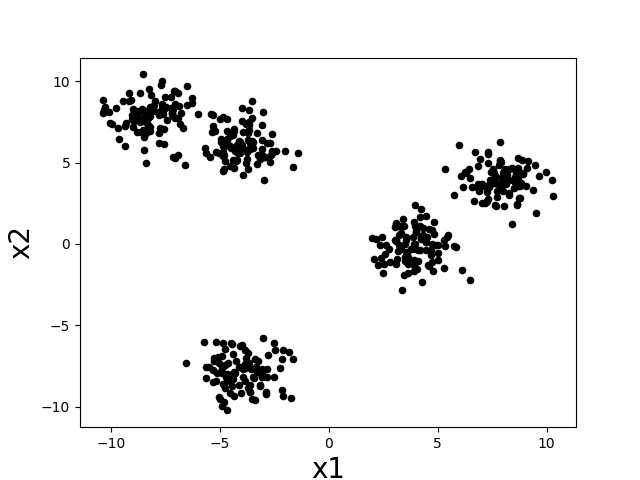
\includegraphics[width=0.40\textwidth]{figures/kmeans_fig1.png}
  \caption{A dataset we would like to cluster. How many clusters do you think there are?}
  \label{fig:kmeans_fig1}
\end{figure}

There seem to be about five clumps of datapoints and those clumps are
what we would like to call clusters. If we assign all datapoints in
each clump to a cluster corresponding to that clump, then we might
desire that nearby datapoints are assigned to the same cluster, while
far apart datapoints are assigned to different clusters.

In designing clustering algorithms, three critical things we need to decide are:
\begin{itemize}
  \item How do we measure \textit{distance} between datapoints? What counts as ``nearby'' and ``far apart''?
  \item How many clusters should we look for?
  \item How do we evaluate how good a clustering is?
\end{itemize}

We will see how to begin making these decisions as we work through a
concrete clustering algorithm in the next section.

\subsection{The k-means formulation}

% Describe with pictures; show good clustering, bad clustering, how do
% we measure? show cluster centers? center pulls in the data. what's
% the objective? here is a reasonable one. quantify dispersal with
% variance --> k-means objective.


% consider showing algorithm first?

One of the simplest and most commonly used clustering algorithms is
called k-means. The goal of the k-means\anchorednote{algorithm}{We
will be careful to distinguish between the k-means {\em algorithm}
and the k-means {\em objective}. As we will see, the k-means
algorithm can be understood to be just one optimization algorithm
which finds a local optimum of the k-means objective.} is to assign
datapoints to $k$ clusters in such a way that
the\anchorednote{variance}{Recall that \textit{variance} is a measure
  of how ``spread out'' data is, defined as the mean squared distance
  from the average value of the data.} within clusters is as small as
possible. Notice that this matches our intuitive idea that a cluster
should be a tightly packed set of datapoints.

Similar to the way we showed that supervised learning could be
formalized mathematically as the minimization of an objective function
(loss function + regularization), we will show how unsupervised
learning can also be formalized as minimizing an objective function.
Let us denote the cluster assignment for a datapoint $x^{(i)}$ as
$y^{(i)} \in \{1,2,\ldots,k\}$, i.e., $y^{(i)} = 1$ means we are
assigning datapoint $x^{(i)}$ to cluster number 1. Then the k-means
objective can be quantified with the following objective function
(which we also call the ``k-means loss''):
\begin{equation}
  \sum_{j=1}^k \sum_{i=1}^n \mathbb{1}(y^{(i)} = j) \left\Vert x^{(i)} - \mu^{(j)} \right\Vert^2 \label{eqn:kmeans_obj} \;,
\end{equation}
where $\mu^{(j)} = \frac{1}{N_j} \sum_{i=1}^n \mathbb{1}(y^{(i)} = j) x^{(i)}$
and $N_j = \sum_{i=1}^n \mathbb{1}(y^{(i)} = j)$, so that $\mu^{(j)}$ is the
mean of all datapoints in cluster $j$, and using $\mathbb{1}(\cdot)$
to denote the indicator function (which takes on value of 1 if its argument
is true and 0 otherwise). The inner sum (over data points) of the loss is
the variance of datapoints within cluster $j$. We sum up the variance
of all $k$ clusters to get our overall loss.\index{k-means!formulation}

\subsection{K-means algorithm}

\index{clustering!k-means algorithm}
The k-means algorithm minimizes this loss by alternating between two
steps: given some initial cluster assignments: 1) compute the mean of
all data in each cluster and assign this as the ``cluster mean'', and 2)
reassign each datapoint to the cluster with nearest cluster
mean. Fig.~\ref{fig:kmeans_iters} shows what happens when we repeat
these steps on the dataset from above.

\begin{figure}[h]
  \centering
  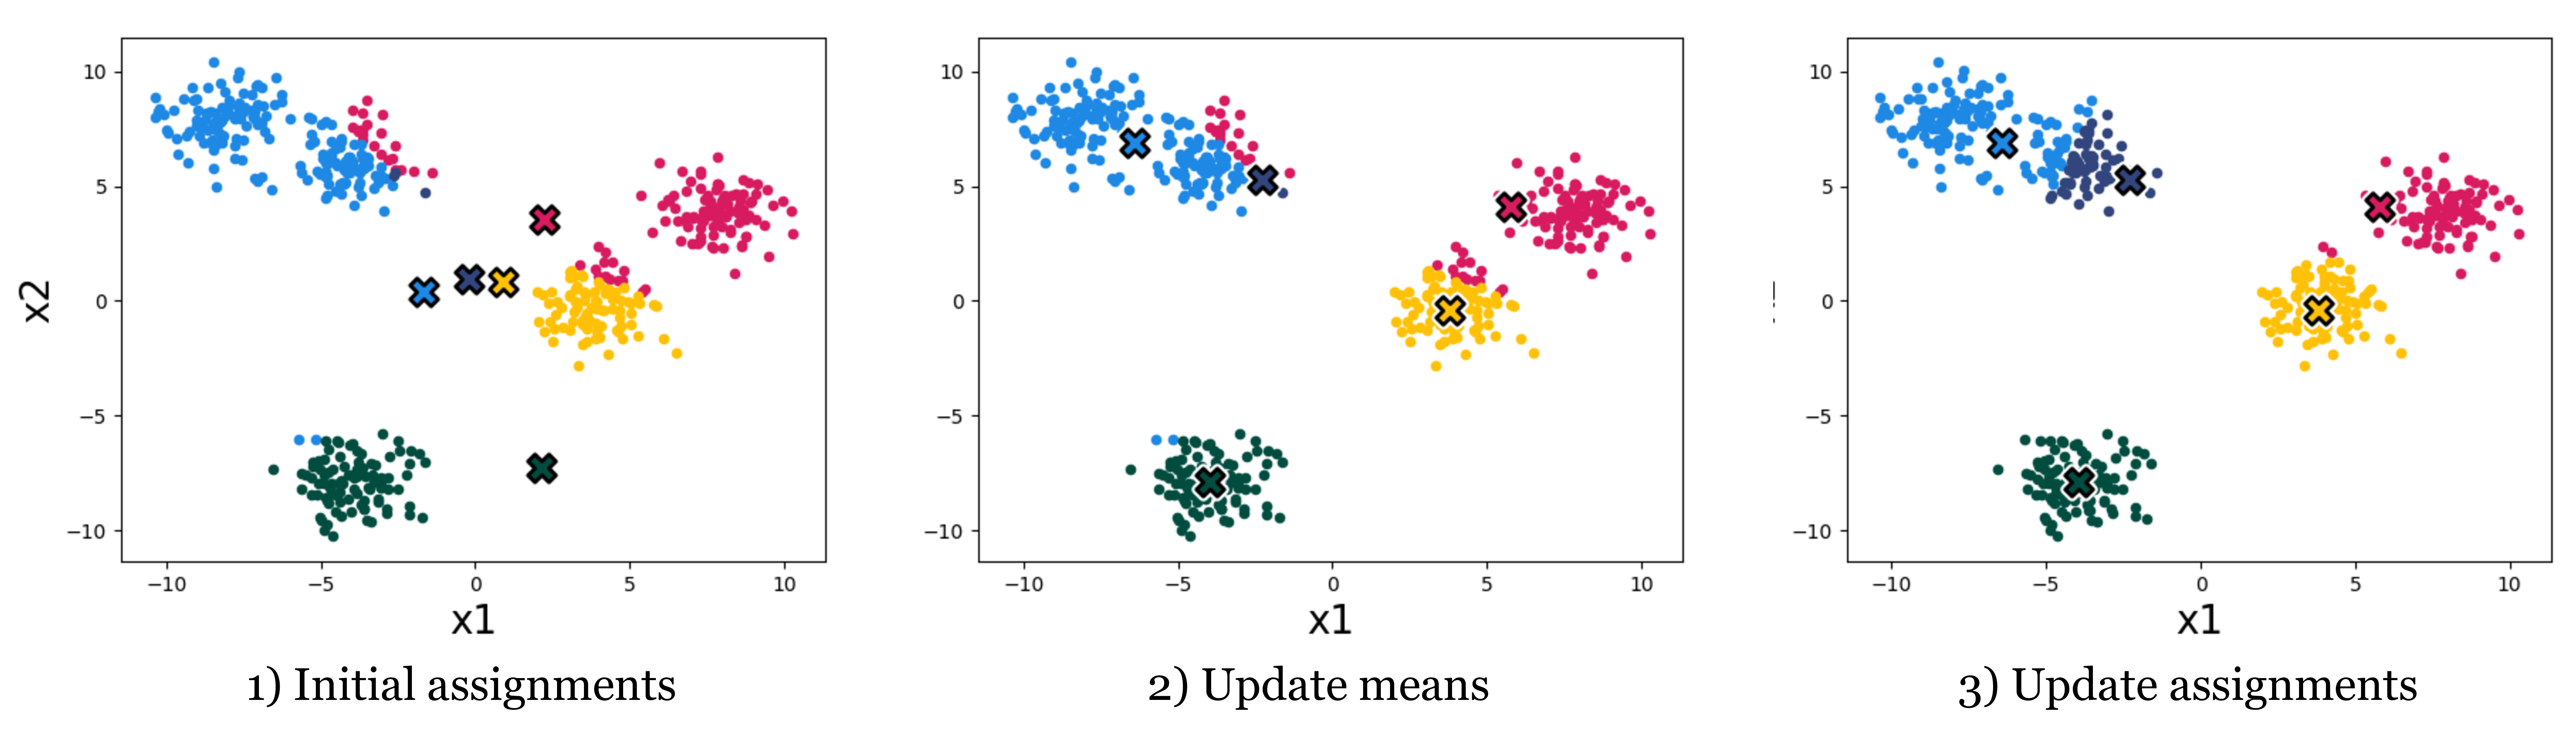
\includegraphics[width=1.0\textwidth]{figures/kmeans_iters.png}
  \caption{The first three steps of running the k-means algorithm on
    this data. Datapoints are colored according to the cluster to
    which they are assigned. Cluster means are the larger X's with
    black outlines.}
  \label{fig:kmeans_iters}
\end{figure}

Each time we reassign the data to the nearest cluster mean, the
k-means loss decreases (the datapoints end up closer to their assigned
cluster mean), or stays the same.  And each time we recompute the
cluster means the loss \textit{also} decreases (the means end up
closer to their assigned datapoints) or stays the same. Overall then,
the clustering gets better and better, according to our objective --
until it stops improving.

After four iterations of cluster assignment + update means in our example,
the k-means algorithm stops improving. Its final solution is shown in Fig.~\ref{fig:kmeans_converged}. It seems to converge to something reasonable!
\begin{figure}[!h]
  \centering
  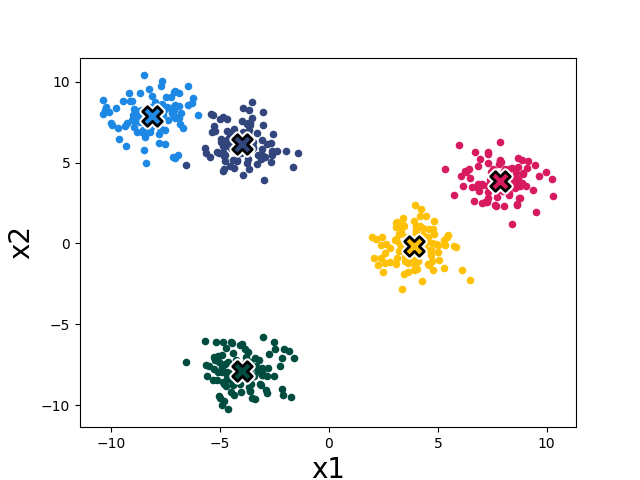
\includegraphics[width=0.38\textwidth]{figures/kmeans_fig2_converged.png}
  \caption{Converged result.}
  \label{fig:kmeans_converged}
\end{figure}

Now let's write out the algorithm in complete detail:
%It can be shown that under mild conditions, this process converges to
%a local minimum of the k-means loss!

%Given some initial assignment of the data to clusters, we first
%compute the mean of all datapoints in each cluster. Then we reassign
%each datapoint to the cluster with the nearest mean. This process
%repeats until convergence.

\begin{codebox}
  \Procname{$\proc{k-means}(k, \tau, \{x^{(i)}\}_{i=1}^n)$}
  \li $\mu, y \gets $ random initialization
  \li \For $t \gets 1$ \To $\tau$
  \li   \Do
  $y_{\texttt{old}} = y$
  \li        \For $i \gets 1$ \To $n$
  \li       \Do
  $y^{(i)} = \arg\min_j \left\Vert x^{(i)} - \mu^{(j)} \right\Vert^2$
  \End
  \li    \For $j \gets 1$ \To $k$
  \li       \Do
  $\mu^{(j)} = \frac{1}{N_j} \sum_{i=1}^n \mathbb{1}(y^{(i)} = j) x^{(i)}$
  \End
  \li      \If $\mathbb{1}(y = y_{\texttt{old}})$
  \li          \Then
  break \label{alg:termination}
  \End
  \End
  \li \Return $\mu, y$
\end{codebox}
\index{k-means!algorithm}
\question{Why do we have the ``break'' statement on
  line~\ref{alg:termination}? Could the clustering improve if we ran
  it for more iterations after this point? Has it converged?}

The for-loop over the $n$ datapoints assigns each datapoint to the
nearest cluster center. The for-loop over the k clusters updates the
cluster center to be the mean of all datapoints currently assigned to
that cluster. As suggested above, it can be shown that this algorithm
reduces the loss in Eq.~\ref{eqn:kmeans_obj} on each iteration, until
it converges to a local minimum of the loss.

% time complexity

It's like classification except it \textit{picked} what the classes
are rather than being given examples of what the classes are.

\subsection{Using gradient descent to minimize k-means objective}

%Study question: could you also minimize the objective with gradient descent?
\index{gradient descent!applied to k-means}
We can also use \anchorednote{gradient descent}{The k-means algorithm
  presented above is a form of \textit{block coordinate descent},
  rather than gradient descent. For certain problems, and in
  particular k-means, this method can converge faster than gradient
  descent.}  to optimize the k-means objective.  To show how to apply
gradient descent, we first rewrite the objective as a differentiable
function \textit{only of} $\mu$:
\begin{equation}
  L(\mu) = \sum_{i=1}^n \min_j \left\Vert x^{(i)} - \mu^{(j)} \right\Vert^2 \;\;.
\end{equation}
$L(\mu)$ is the value of the k-means loss given that we pick the
\textit{optimal} assignments of the datapoints to cluster means
(that's what the $\min_j$ does). Now we can use the
gradient\anchorednote{$\frac{\partial L(\mu)}{\partial \mu}$}{$L(\mu)$
  is a smooth function except with kinks where the nearest cluster
  changes; that means it's differentiable almost everywhere, which in
  practice is sufficient for us to apply gradient descent.} to find
the values for $\mu$ that achieve minimum loss when cluster
assignments are optimal.  Finally, we read off the optimal cluster
assignments, given the optimized $\mu$, just by assigning datapoints
to their nearest cluster mean:
\begin{equation}
  y^{(i)} = \arg\min_j \left\Vert x^{(i)} - \mu^{(j)} \right\Vert^2 \;\;.
\end{equation}
This procedure yields a local minimum of Eq.~\ref{eqn:kmeans_obj}, as
does the standard k-means algorithm we presented (though they might
arrive at different solutions). It might not be the global optimum
since the objective is not convex (due to $\min_j$, as the minimum of
multiple convex functions is not necessarily convex).

% mention sub-gradient
% figure out if this is ever done in practice
% say it is not typical

% previous algorithm is block coordinate descent

\subsection{Importance of initialization}
The standard k-means algorithm, as well as the variant that uses
gradient descent, both are only guaranteed to converge to a local
minimum, not necessarily the global minimum of the loss. Thus the
answer we get out depends on how we initialize the cluster
means. Figure~\ref{fig:kmeans_init} is an example of a different
initialization on our toy data, which results in a worse converged
clustering:\index{k-means!initialization}

\begin{figure}[h]
  \centering
  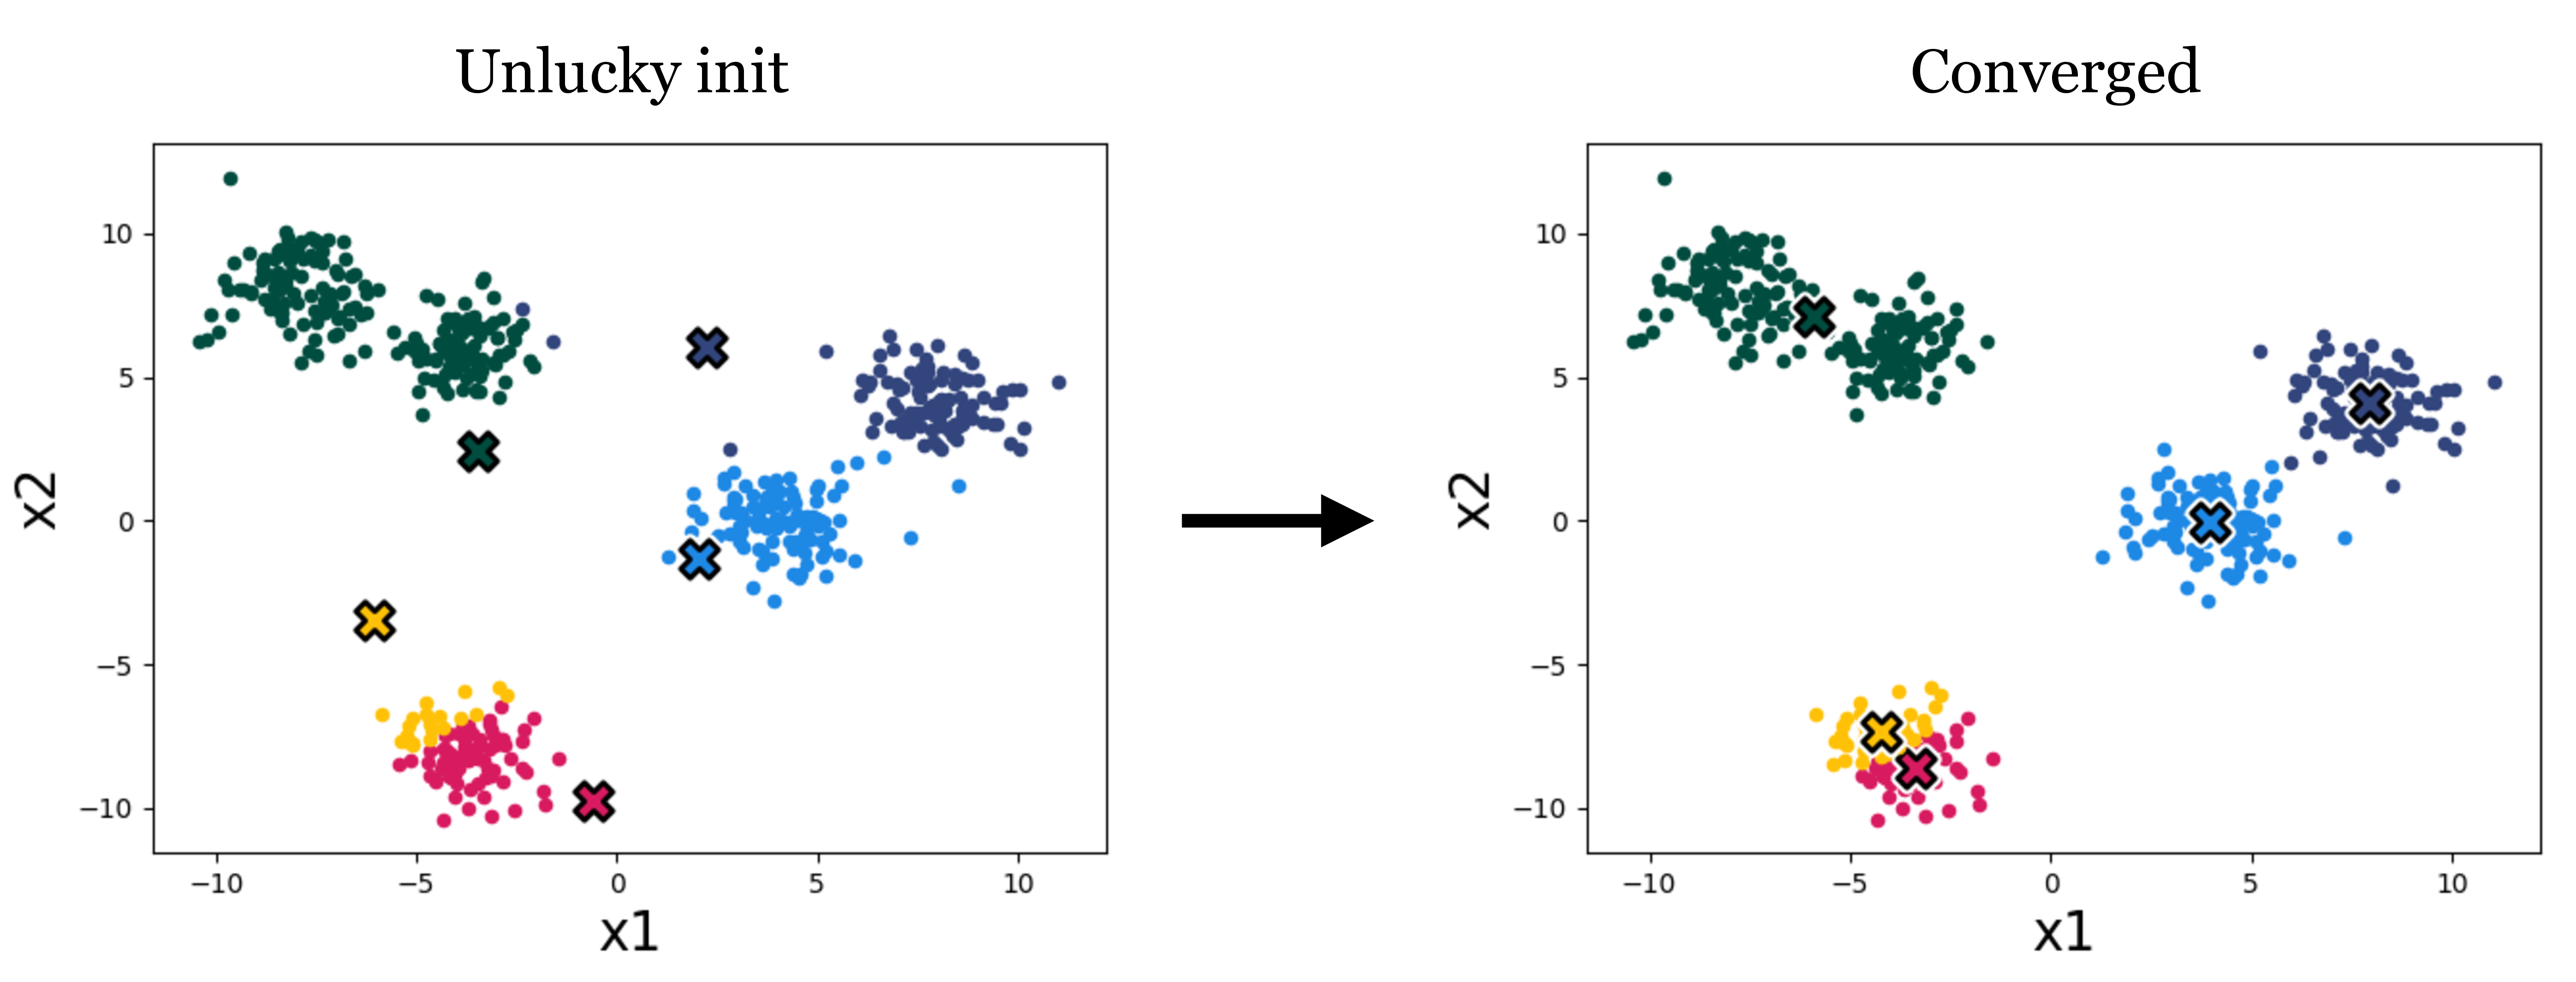
\includegraphics[width=0.8\textwidth]{./figures/kmeans_init.png}
  \caption{With the initialization of the means to the left, the
    yellow and red means end up splitting what perhaps should be one
    cluster in half.}
  \label{fig:kmeans_init}
\end{figure}

A variety of methods have been developed to pick good initializations
(see, for example, the \textit{k-means++} algorithm). One simple
option is to run the standard k-means algorithm multiple times, with
different random initial conditions, and then pick from these the
clustering that achieves the lowest k-means loss.

\subsection{Importance of k}\label{sec-importance_of_k}

A very important parameter in cluster algorithms is the number of
clusters we are looking for. Some advanced algorithms can
automatically infer a suitable number of clusters, but most of the
time, like with k-means, we will have to pick $k$ -- it's a
hyperparameter of the algorithm.

\begin{figure}[h]
  \centering
  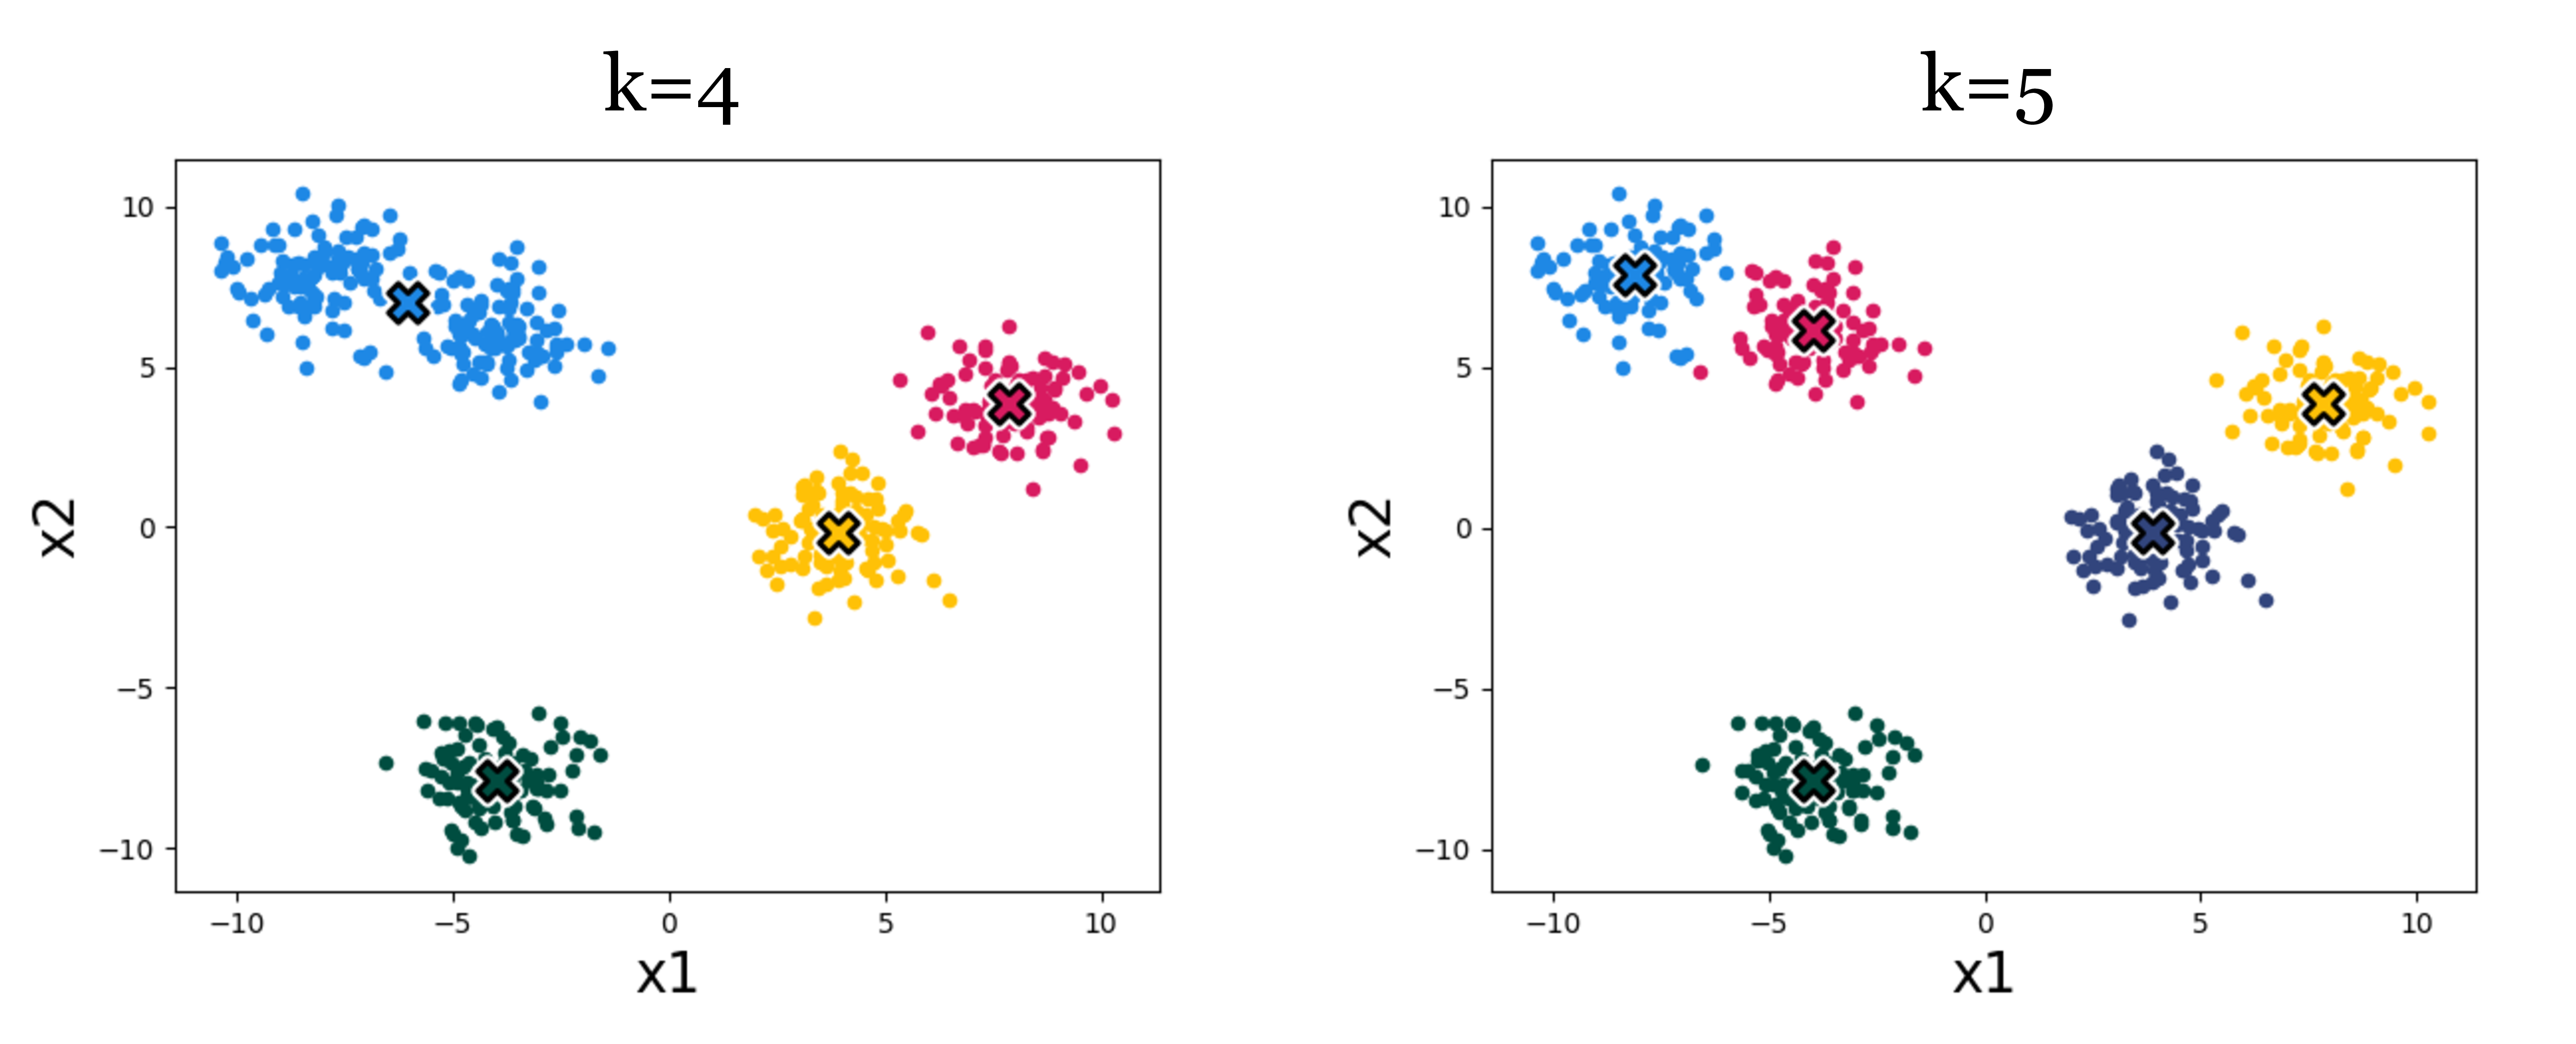
\includegraphics[width=0.67\textwidth]{figures/effect_of_k.png}
  \caption{Example of k-means run on our toy data, with two
    different values of k. Setting k=4, on the left, results in one
    cluster being merged, compared to setting k=5, on the
    right. Which clustering do you think is better? How could you
    decide?}
  \label{fig:effect_of_k}
\end{figure}

Figure~\ref{fig:effect_of_k} shows an example of the effect.  Which
result looks more correct? It can be hard to say! Using higher k we
get more clusters, and with more clusters we can achieve lower
within-cluster variance -- the k-means objective will never increase,
and will typically strictly decrease as we increase k. Eventually, we
can increase k to equal the total number of datapoints, so that each
datapoint is assigned to its own cluster. Then the k-means objective
is zero, but the clustering reveals nothing.  Clearly, then, we cannot
use the k-means objective itself to choose the best value for k. In subsection~\ref{sec-eval}, we will discuss some ways of evaluating the
success of clustering beyond its ability to minimize the k-means
objective, and it's with these sorts of methods that we might decide
on a proper value of k.

Alternatively, you may be wondering: why bother picking a single k?
Wouldn't it be nice to reveal a \textit{hierarchy} of clusterings of
our data, showing both coarse and fine groupings? Indeed
\textit{hierarchical clustering} \index{hierarchical clustering} is another important class of
clustering algorithms, beyond k-means. These methods can be useful for
discovering tree-like structure in data, and they work a bit like this: initially a coarse
split/clustering of the data is applied at the root of the tree, and then as we
descend the tree we split and cluster the data in ever more fine-grained ways. A
prototypical example of hierarchical clustering is to discover a
taxonomy of life, where creatures may be grouped at multiple
granularities, from species to families to kingdoms.


% the
% decision trees we will see later in Chapter~\ref{chap-nonparametric},
% point out: there may be no right answer
%   -- hierarchical call out (different granularities)

% btw there exists a class that finds the whole hierarchy...
% hint at the breadth but focus on k-means

% forge connections to previous topics 
%   -- decision trees and nearest-neighbors
%   -- feature space, autoencoder

\subsection{k-means in feature space}

Clustering algorithms group data based on a notion of
\textit{similarity}, and thus we need to define a \textit{distance metric}
between datapoints. This notion
will also be useful in other machine learning approaches,
such as nearest-neighbor methods that we see in Chapter~\ref{chap-nonparametric}.
In k-means and other methods, our choice of distance
metric can have a big impact on the results we will find.

Our k-means algorithm uses the Euclidean distance, i.e., $\left\Vert
  x^{(i)} - \mu^{(j)} \right\Vert$, with a loss function that is the
square of this distance. We can modify k-means to use different
distance metrics, but a more common trick is to stick with Euclidean
distance but measured in a \textit{feature space}. Just like we did
for regression and classification problems, we can define a feature
map from the data to a nicer feature representation, $\phi(x)$, and
then apply k-means to cluster the data in the\anchorednote{feature
  space.}{In fact, using a simple distance metric in feature space can
  be equivalent to using a more sophisticated distance metric in the
  data space, and this trick forms the basis of \textit{kernel
    methods}, which you can learn about in more advanced machine
  learning classes.}\index{k-means!in feature space}

As a simple example, suppose we have two-dimensional data that is very
stretched out in the first dimension and has less dynamic range in the
second dimension. Then we may want to scale the dimensions so that
each has similar dynamic range, prior to clustering. We could use
standardization, like we did in Chapter~\ref{chap-features}.

If we want to cluster more complex data, like images, music, chemical
compounds, etc., then we will usually need more sophisticated feature
representations. One common practice these days is to use feature
representations learned with a neural network. For example, we can use
an autoencoder to compress images into feature vectors, then cluster
those feature vectors.

%it's best to use a nice feature representation of the data rather
%than the raw format stored on your computer

%As an example, we could use an autoencoder to get the features, as shown here:
% \begin{figure}[h]
%     \centering
%     \includegraphics[width=0.33\textwidth]{example-image-a}
%     \caption{Example of k-means run on some data, in different feature spaces, raw data vs. autoencoder features.}
%     \label{fig:my_label}
% \end{figure}
% connects to week 11's hw too

\subsubsection{How to evaluate clustering algorithms}
\label{sec-eval}

\index{clustering!evaluation}
One of the hardest aspects of clustering is knowing how to evaluate
it. This is actually a big issue for all unsupervised learning
methods, since we are just looking for patterns in the data, rather
than explicitly trying to predict target values (which was the case
with supervised learning).

Remember, evaluation metrics are \textit{not} the same as loss
functions, so we can't just measure success by looking at the k-means
loss. In prediction problems, it is critical that the evaluation is on
a held-out test set, while the loss is computed over training data. If
we evaluate on training data we cannot detect overfitting. Something
similar is going on with the example in
Section~\ref{sec-importance_of_k}, where setting k to be too large can
precisely ``fit'' the data (minimize the loss), but yields no general
insight.

One way to evaluate our clusters is to look at the
\textbf{consistency} with which they are found when we run on
different subsamples of our training data, or with different
hyperparameters of our clustering algorithm (e.g.,
initializations). For example, if running on several bootstrapped
samples (random subsets of our data) results in very different
clusters, it should call into question the validity of any of the
individual results.

If we have some notion of what \textbf{ground truth} clusters should
be, e.g., a few data points that we know should be in the same
cluster, then we can measure whether or not our discovered clusters
group these examples correctly.

Clustering is often used for \textbf{visualization} and
\textbf{interpretability}, to make it easier for humans to understand
the data. Here, human judgment may guide the choice of clustering
algorithm. More quantitatively, discovered clusters may be used as input to
\textbf{downstream tasks}. For example, as we saw in the lab, we may fit a different
regression function on the data within each
cluster. Figure~\ref{fig:simpsons_color} gives
an example where this might be useful. In cases like this, the success
of a clustering algorithm can be indirectly measured based on the
success of the downstream application (e.g., does it make the
downstream predictions more accurate).

\begin{figure}[h]
  \centering
  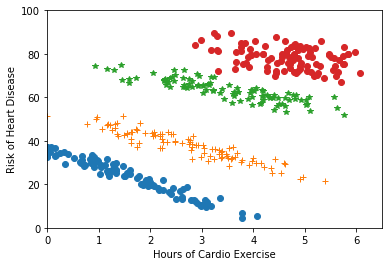
\includegraphics[width=0.35\textwidth]{figures/simpsons_color.png}
  \caption{Averaged across the whole population, risk of heart
    disease positively correlates with hours of exercise. However,
    if we cluster the data, we can observe that there are four
    subgroups of the population which correspond to different age
    groups, and within each subgroup the correlation is negative. We
    can make better predictions, and better capture the presumed
    true effect, if we cluster this data and then model the trend in
    each cluster separately.}
  \label{fig:simpsons_color}
\end{figure}

% Fun stuff to end on?
% High level about unsupervised learning?

% \section{Applications of clustering}

% Clustering has many applications, from visualizing and understanding
% data to efficiently transmitting data over the Internet. Here are a
% few you are now equipped to learn about:

% \begin{itemize}
%     \item ``Vector quantization'' and compression: if we have high-dimensional feature vectors we can summarize them with more compact codewords, i.e., cluster assignments. 
%     \item 
% \end{itemize}

% applications
%  vector quantization; compression

%%% Local Variables:
%%% mode: latex
%%% TeX-master: "top"
%%% End:




\section{Autoencoder structure}
\label{chap-autoencoders}
Assume that we have input data $\mathcal{D} = \{x^{(1)}, \ldots,
  x^{(n)} \}$, where $x^{(i)}\in \mathbb{R}^d$. We seek to learn an
autoencoder that will output a new dataset $\mathcal{D}_{out} =
  \{a^{(1)}, \ldots, a^{(n)}\}$, where $a^{(i)}\in \mathbb{R}^k$ with $k
  < d$. We can think about $a^{(i)}$ as the new \textit{representation}
of data point $x^{(i)}$. For example, in Fig.~\ref{fig:illustration}
we show the learned representations of a dataset of MNIST digits with
$k=2$. We see, after inspecting the individual data points, that
unsupervised learning has found a compressed (or {\em latent}\index{latent representation})
representation where images of the same digit are close to each
other, potentially greatly aiding subsequent clustering or
classification tasks.

\begin{figure}[h!]
  \centering
  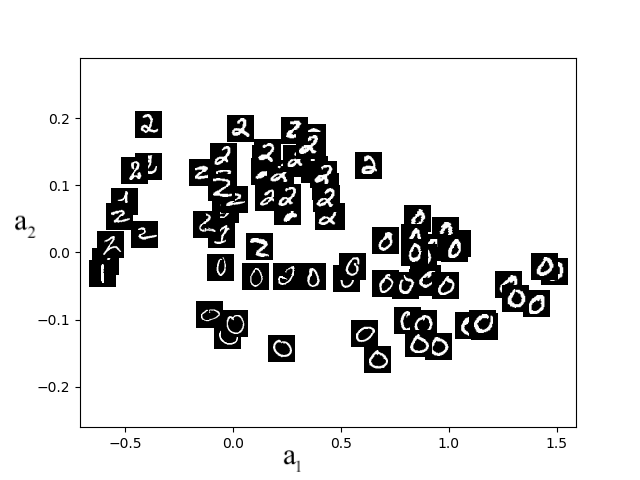
\includegraphics[width= .5\textwidth]{figures/autoencoder_mnist.png}
  \caption{\small Compression of digits dataset into two
    dimensions. The input $x^{(i)}$, an image of a handwritten
    digit, is shown at the new low-dimensional representation
    $(a_1,a_2)$.}
  \label{fig:illustration}
\end{figure}

Formally, an autoencoder consists of two functions, a vector-valued
\textit{encoder} $g : \mathbb{R}^d \rightarrow \mathbb{R}^k$ that
deterministically maps the data to the representation space $a \in
  \mathbb{R}^k$, and a \textit{decoder} $h : \mathbb{R}^k \rightarrow
  \mathbb{R}^d$ that maps the representation space back into the
original data space.

In general, the encoder and decoder functions might be any functions
appropriate to the domain. Here, we are particularly interested in
neural network embodiments of encoders and decoders.
The basic architecture of one such autoencoder, consisting of only a single
layer neural network in each of the encoder and decoder, is shown in
Figure~\ref{fig:autoencoder}; note that bias terms $W^1_0$ and $W^2_0$ into
the summation nodes exist, but are omitted for clarity in the figure.
In this example, the original
$d$-dimensional input is compressed into $k=3$ dimensions via the
encoder $g(x; W^1, W^1_0)=f_1(W{^1}^T x + W^1_0)$ with $W^1 \in
  \mathbb{R}^{d \times k}$ and $W^1_0 \in \mathbb{R}^k$,
and where the non-linearity $f_1$ is applied to each
dimension of the vector. To recover (an approximation to) the
original instance, we then apply the decoder $h(a; W^2, W^2_0) = f_2(W{^2}^T
  a + W^2_0)$, where $f_2$ denotes a different non-linearity (activation
function). In general, both the decoder and the encoder could involve
multiple layers, as opposed to the single layer shown here. Learning
seeks parameters $W^1, W^1_0$ and $W^2, W^2_0$ such that the reconstructed
instances, $h(g(x^{(i)}; W^{1}, W^1_0); W^{2}, W^2_0)$, are close to the original
input $x^{(i)}.$

\begin{figure}[h]
  \centering
  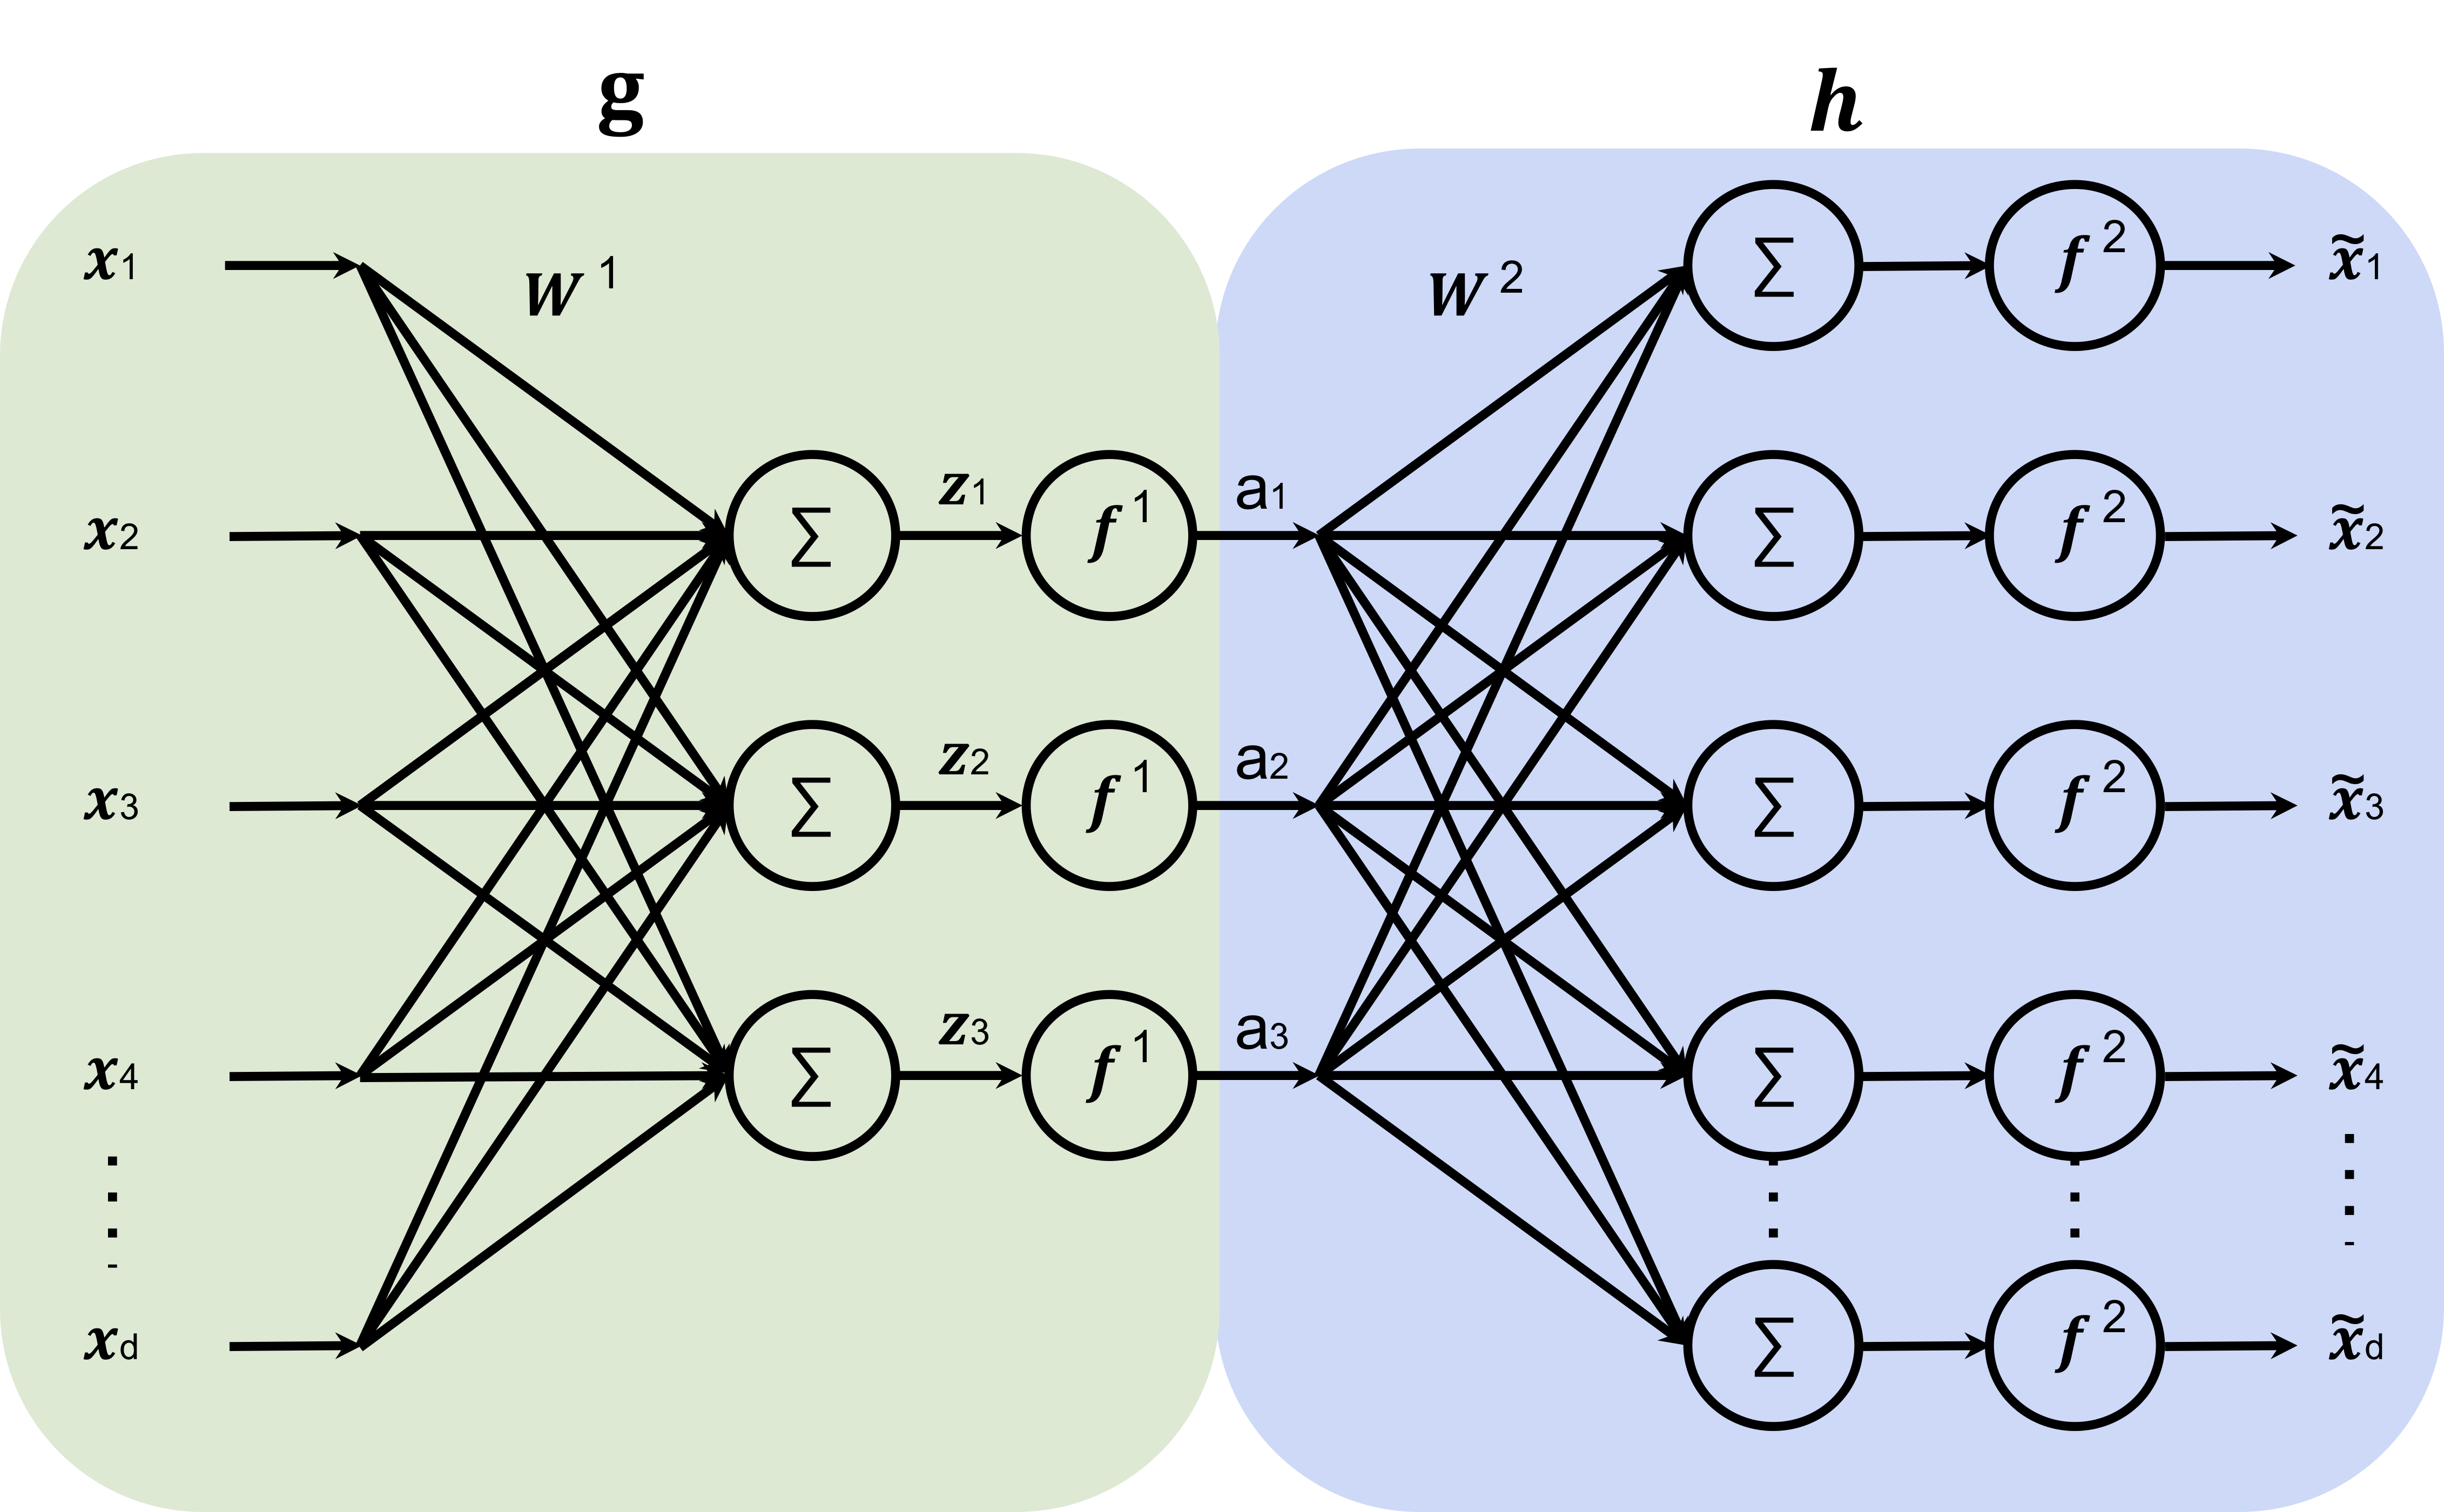
\includegraphics[width=.7\textwidth]{figures/autoencoder.png}
  \caption{\small Autoencoder structure, showing the encoder (left
    half, light green), and the decoder (right half, light blue),
    encoding inputs $x$ to the representation $a$, and decoding the
    representation to produce $\tilde{x}$, the reconstruction.  In
    this specific example, the representation ($a_1$, $a_2$, $a_3$)
    only has three dimensions.\label{fig:autoencoder}}
\end{figure}

\subsection{Autoencoder Learning}

We learn the weights in an autoencoder using the same tools that we previously used for
supervised learning, namely (stochastic) gradient descent of a
multi-layer neural network to minimize a loss function. All that
remains is to specify the loss function $\mathcal{L}(\tilde{x}, x)$, which tells
us how to measure the discrepancy between the reconstruction
$\tilde{x} = h(g(x; W^{1}, W^1_0); W^{2}, W^2_0)$ and the original input $x$. For
example, for continuous-valued $x$ it might make sense to use squared
loss, i.e., $\mathcal{L}_{SE}(\tilde{x}, x) = \sum_{j=1}^{d} (x_j -
  \tilde{x}_j)^2$.\note{Alternatively, you could think of this as {\em
      multi-task learning}, where the goal is to predict each dimension
  of $x$. One can mix-and-match loss functions as appropriate for each
  dimension's data type.} Learning then seeks to optimize the
parameters of $h$ and $g$ so as to minimize the reconstruction error,
measured according to this loss function:
\[
  \min_{W^{1}, W^1_0, W^{2}, W^2_0} \sum_{i=1}^n \mathcal{L}_{SE}\left(h(g(x^{(i)}; W^{1}, W^1_0); W^{2}, W^2_0), x^{(i)}\right)
\]

\subsection{Evaluating an autoencoder}

What makes a good learned representation in an autoencoder? Notice
that, without further constraints, it is always possible to perfectly
reconstruct the input. For example, we could let $k=d$ and $h$ and $g$
be the identity functions. In this case, we would not obtain any
compression of the data.

To learn something useful, we must create a
\textit{bottleneck} by making $k$ to be smaller (often much smaller)
than $d$. This forces the learning algorithm to seek transformations
that describe the original data using as simple a description as
possible. Thinking back to the digits dataset, for example, an example
of a compressed representation might be the digit label (i.e., 0--9),
rotation, and stroke thickness. Of course, there is no guarantee that
the learning algorithm will discover precisely this
representation. After learning, we can inspect the learned
representations, such as by artificially increasing or decreasing one
of the dimensions (e.g., $a_1$) and seeing how it affects the output
$h(a)$, to try to better understand what it has learned.

As with clustering, autoencoders can be a preliminary step toward
building other models, such as a regressor or classifier. For example,
once a good encoder has been learned, the decoder might be replaced
with another neural network that is then trained with supervised learning
(perhaps using a smaller dataset that does include labels).

\subsection{Linear encoders and decoders}

We close by mentioning that even linear encoders and decoders can be
very powerful. In this case, rather than minimizing the above
objective with gradient descent, a technique called \textit{principal
  components analysis} (PCA) can be used to obtain a closed-form
solution to the optimization problem using a singular value
decomposition (SVD).  Just as a multilayer neural network with
nonlinear activations for regression (learned by gradient descent) can
be thought of as a nonlinear generalization of a linear regressor (fit
by matrix algebraic operations), the neural network based autoencoders
discussed above (and learned with gradient descent) can be thought of
as a generalization of linear PCA (as solved with matrix algebra by
SVD).

\subsection{Advanced encoders and decoders}

Advanced neural networks that build on the encoder-decoder conceptual
decomposition have become increasingly powerful in recent years. One
family of applications are {\em generative}\index{generative networks}
networks, where new outputs that are ``similar to'' but different from
any existing training sample are desired. In {\em variational
    autoencoders}\index{autoencoder!variational} the compressed
representation encompasses information about the probability
distribution of training samples, e.g., learning both mean and
standard deviation variables in the bottleneck layer or latent
representation. Then, new outputs can be generated by random sampling
based on the latent representation variables and feeding those samples
into the decoder. For instance, {\em Transformers} use {\em multiple} encoder and
decoder blocks, together with a self-attention mechanism to make predictions
about potential next outputs resulting from sequences of inputs. Such
transformer networks have many applications in natural language
processing and elsewhere.


% \chapter{Clustering}
\label{chap-clustering}

Oftentimes a dataset can be partitioned into different categories. A
doctor may notice that their patients come in cohorts and different
cohorts respond to different treatments. A biologist may gain insight
by identifying that bats and whales, despite outward appearances,
have some underlying similarity, and both should be considered members
of the same category, i.e., ``mammal''. The problem of automatically
identifying meaningful groupings in datasets is called
clustering. Once these groupings are found, they can be leveraged
toward interpreting the data and making optimal decisions for each
group.
\index{clustering}

\section{Clustering formalisms}

%Imagine that you are a scientist studying the human genome.

%Sometimes data seems to come in different categories. How can we
%identify these categories, and thereby treat them specifically? We
%call these categories clusters.

%Mathematically, clustering is the problem of \textit{partitioning} a
%dataset $\{x_i\}_{i=1}^n$ such that each datapoint is assigned to one
%partition.

Mathematically, clustering looks a bit like classification: we wish to
find a mapping from datapoints, $x$, to categories, $y$. However,
rather than the categories being predefined labels, the categories in
clustering are automatically discovered \textit{partitions} of an
unlabeled dataset.\index{clustering!into partitions}

Because clustering does not learn from labeled examples, it is an
example of an \textit{unsupervised} learning algorithm. Instead of
mimicking the mapping implicit in supervised training pairs
$\{x^{(i)},y^{(i)}\}_{i=1}^n$, clustering assigns datapoints to
categories based on how the unlabeled data $\{x^{(i)}\}_{i=1}^n$ is
\textit{distributed} in data space.

%, which can be indexed by the integers, $\mathbb{Z}$. That is, in
%both classification and clustering, we learn $f: \mathbb{R}^N
%\rightarrow \mathbb{Z}$.

%The difference between clustering and classification is in the
%objective function. Classification is supervised -- we simply map
%datapoints to categories in a way that matches training examples
%$\{x^{(i)},y^{(i)}\}_{i=1}^n$. Clustering, on the other hand, is
%\textit{unsupervised}: we are only given unlabeled datapoints
%$\{x^{(i)}\}_{i=1}^n$, and we have to decide which datapoints belong
%to which categories based on how the data is \textit{distributed} in
%data space.

Intuitively, a ``cluster'' is a group of datapoints that are all
nearby to each other and far away from other clusters. Let's consider
the following scatter plot. How many clusters do you think there are?

\begin{figure}[h]
  \centering
  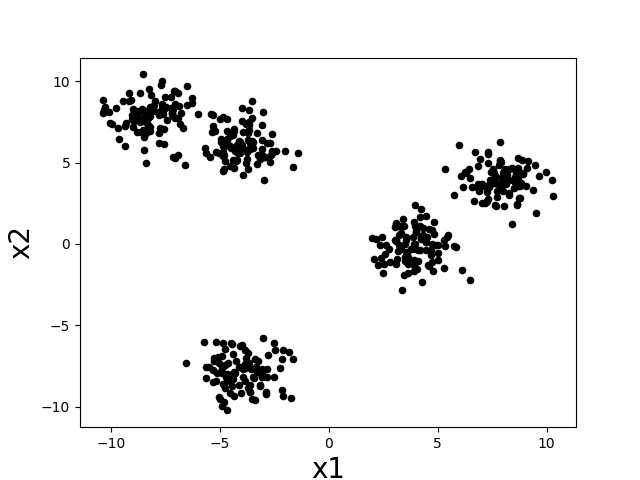
\includegraphics[width=0.40\textwidth]{figures/kmeans_fig1.png}
  \caption{A dataset we would like to cluster. How many clusters do you think there are?}
  \label{fig:kmeans_fig1}
\end{figure}

There seem to be about five clumps of datapoints and those clumps are
what we would like to call clusters. If we assign all datapoints in
each clump to a cluster corresponding to that clump, then we might
desire that nearby datapoints are assigned to the same cluster, while
far apart datapoints are assigned to different clusters.

In designing clustering algorithms, three critical things we need to decide are:
\begin{itemize}
  \item How do we measure \textit{distance} between datapoints? What counts as ``nearby'' and ``far apart''?
  \item How many clusters should we look for?
  \item How do we evaluate how good a clustering is?
\end{itemize}

We will see how to begin making these decisions as we work through a
concrete clustering algorithm in the next section.

\section{The k-means formulation}

% Describe with pictures; show good clustering, bad clustering, how do
% we measure? show cluster centers? center pulls in the data. what's
% the objective? here is a reasonable one. quantify dispersal with
% variance --> k-means objective.


% consider showing algorithm first?

One of the simplest and most commonly used clustering algorithms is
called k-means. The goal of the k-means\anchorednote{algorithm}{We
will be careful to distinguish between the k-means {\em algorithm}
and the k-means {\em objective}. As we will see, the k-means
algorithm can be understood to be just one optimization algorithm
which finds a local optimum of the k-means objective.} is to assign
datapoints to $k$ clusters in such a way that
the\anchorednote{variance}{Recall that \textit{variance} is a measure
  of how ``spread out'' data is, defined as the mean squared distance
  from the average value of the data.} within clusters is as small as
possible. Notice that this matches our intuitive idea that a cluster
should be a tightly packed set of datapoints.

Similar to the way we showed that supervised learning could be
formalized mathematically as the minimization of an objective function
(loss function + regularization), we will show how unsupervised
learning can also be formalized as minimizing an objective function.
Let us denote the cluster assignment for a datapoint $x^{(i)}$ as
$y^{(i)} \in \{1,2,\ldots,k\}$, i.e., $y^{(i)} = 1$ means we are
assigning datapoint $x^{(i)}$ to cluster number 1. Then the k-means
objective can be quantified with the following objective function
(which we also call the ``k-means loss''):
\begin{equation}
  \sum_{j=1}^k \sum_{i=1}^n \mathbb{1}(y^{(i)} = j) \left\Vert x^{(i)} - \mu^{(j)} \right\Vert^2 \label{eqn:kmeans_obj} \;,
\end{equation}
where $\mu^{(j)} = \frac{1}{N_j} \sum_{i=1}^n \mathbb{1}(y^{(i)} = j) x^{(i)}$
and $N_j = \sum_{i=1}^n \mathbb{1}(y^{(i)} = j)$, so that $\mu^{(j)}$ is the
mean of all datapoints in cluster $j$, and using $\mathbb{1}(\cdot)$
to denote the indicator function (which takes on value of 1 if its argument
is true and 0 otherwise). The inner sum (over data points) of the loss is
the variance of datapoints within cluster $j$. We sum up the variance
of all $k$ clusters to get our overall loss.\index{k-means!formulation}

\subsection{K-means algorithm}

\index{clustering!k-means algorithm}
The k-means algorithm minimizes this loss by alternating between two
steps: given some initial cluster assignments: 1) compute the mean of
all data in each cluster and assign this as the ``cluster mean'', and 2)
reassign each datapoint to the cluster with nearest cluster
mean. Fig.~\ref{fig:kmeans_iters} shows what happens when we repeat
these steps on the dataset from above.

\begin{figure}[h]
  \centering
  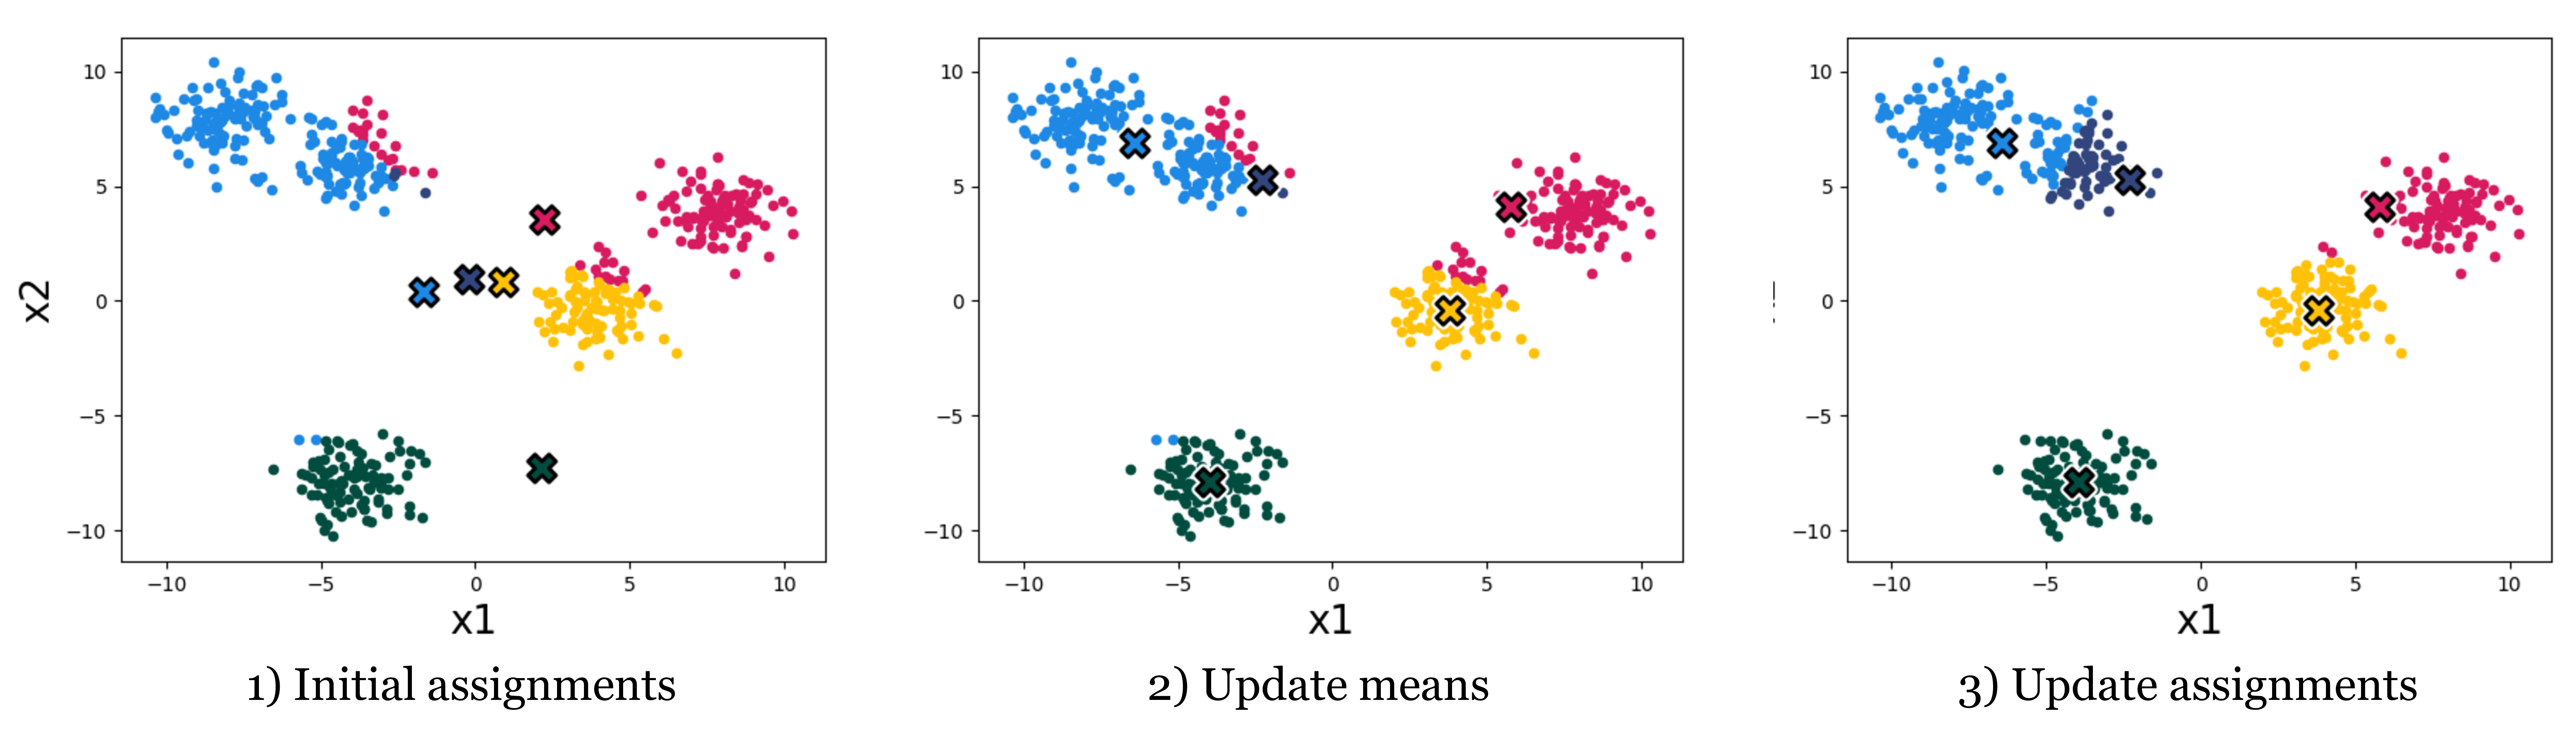
\includegraphics[width=1.0\textwidth]{figures/kmeans_iters.png}
  \caption{The first three steps of running the k-means algorithm on
    this data. Datapoints are colored according to the cluster to
    which they are assigned. Cluster means are the larger X's with
    black outlines.}
  \label{fig:kmeans_iters}
\end{figure}

Each time we reassign the data to the nearest cluster mean, the
k-means loss decreases (the datapoints end up closer to their assigned
cluster mean), or stays the same.  And each time we recompute the
cluster means the loss \textit{also} decreases (the means end up
closer to their assigned datapoints) or stays the same. Overall then,
the clustering gets better and better, according to our objective --
until it stops improving.

After four iterations of cluster assignment + update means in our example,
the k-means algorithm stops improving. We say it has converged,
and its final solution is shown in Fig.~\ref{fig:kmeans_converged}.
\begin{figure}[h]
  \centering
  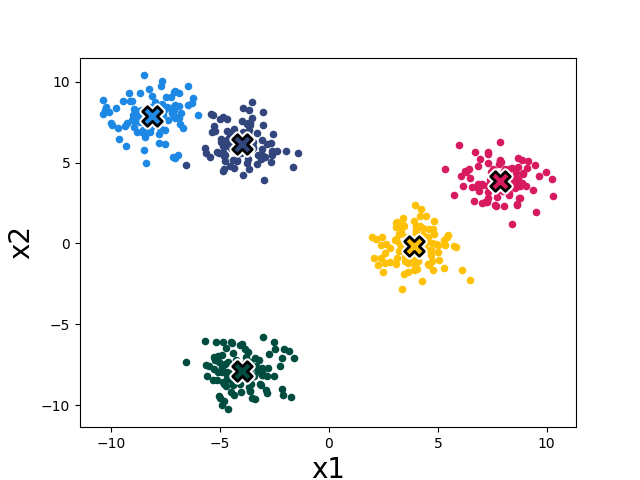
\includegraphics[width=0.4\textwidth]{figures/kmeans_fig2_converged.png}
  \caption{Converged result.}
  \label{fig:kmeans_converged}
\end{figure}

It seems to converge to something reasonable! Now let's write out the
algorithm in complete detail:
%It can be shown that under mild conditions, this process converges to
%a local minimum of the k-means loss!

%Given some initial assignment of the data to clusters, we first
%compute the mean of all datapoints in each cluster. Then we reassign
%each datapoint to the cluster with the nearest mean. This process
%repeats until convergence.

\begin{codebox}
  \Procname{$\proc{k-means}(k, \tau, \{x^{(i)}\}_{i=1}^n)$}
  \li $\mu, y \gets $ random initialization
  \li \For $t \gets 1$ \To $\tau$
  \li   \Do
  $y_{\texttt{old}} = y$
  \li        \For $i \gets 1$ \To $n$
  \li       \Do
  $y^{(i)} = \arg\min_j \left\Vert x^{(i)} - \mu^{(j)} \right\Vert^2$
  \End
  \li    \For $j \gets 1$ \To $k$
  \li       \Do
  $\mu^{(j)} = \frac{1}{N_j} \sum_{i=1}^n \mathbb{1}(y^{(i)} = j) x^{(i)}$
  \End
  \li      \If $\mathbb{1}(y = y_{\texttt{old}})$
  \li          \Then
  break \label{alg:termination}
  \End
  \End
  \li \Return $\mu, y$
\end{codebox}
\index{k-means!algorithm}
\question{Why do we have the ``break'' statement on
  line~\ref{alg:termination}? Could the clustering improve if we ran
  it for more iterations after this point? Has it converged?}

The for-loop over the $n$ datapoints assigns each datapoint to the
nearest cluster center. The for-loop over the k clusters updates the
cluster center to be the mean of all datapoints currently assigned to
that cluster. As suggested above, it can be shown that this algorithm
reduces the loss in Eq.~\ref{eqn:kmeans_obj} on each iteration, until
it converges to a local minimum of the loss.

% time complexity

It's like classification except it \textit{picked} what the classes
are rather than being given examples of what the classes are.

\subsection{Using gradient descent to minimize k-means objective}

%Study question: could you also minimize the objective with gradient descent?
\index{gradient descent!applied to k-means}
We can also use \anchorednote{gradient descent}{The k-means algorithm
  presented above is a form of \textit{block coordinate descent},
  rather than gradient descent. For certain problems, and in
  particular k-means, this method can converge faster than gradient
  descent.}  to optimize the k-means objective.  To show how to apply
gradient descent, we first rewrite the objective as a differentiable
function \textit{only of} $\mu$:
\begin{equation}
  L(\mu) = \sum_{i=1}^n \min_j \left\Vert x^{(i)} - \mu^{(j)} \right\Vert^2 \;\;.
\end{equation}
$L(\mu)$ is the value of the k-means loss given that we pick the
\textit{optimal} assignments of the datapoints to cluster means
(that's what the $\min_j$ does). Now we can use the
gradient\anchorednote{$\frac{\partial L(\mu)}{\partial \mu}$}{$L(\mu)$
  is a smooth function except with kinks where the nearest cluster
  changes; that means it's differentiable almost everywhere, which in
  practice is sufficient for us to apply gradient descent.} to find
the values for $\mu$ that achieve minimum loss when cluster
assignments are optimal.  Finally, we read off the optimal cluster
assignments, given the optimized $\mu$, just by assigning datapoints
to their nearest cluster mean:
\begin{equation}
  y^{(i)} = \arg\min_j \left\Vert x^{(i)} - \mu^{(j)} \right\Vert^2 \;\;.
\end{equation}
This procedure yields a local minimum of Eq.~\ref{eqn:kmeans_obj}, as
does the standard k-means algorithm we presented (though they might
arrive at different solutions). It might not be the global optimum
since the objective is not convex (due to $\min_j$, as the minimum of
multiple convex functions is not necessarily convex).

% mention sub-gradient
% figure out if this is ever done in practice
% say it is not typical

% previous algorithm is block coordinate descent

\subsection{Importance of initialization}
The standard k-means algorithm, as well as the variant that uses
gradient descent, both are only guaranteed to converge to a local
minimum, not necessarily the global minimum of the loss. Thus the
answer we get out depends on how we initialize the cluster
means. Figure~\ref{fig:kmeans_init} is an example of a different
initialization on our toy data, which results in a worse converged
clustering:\index{k-means!initialization}

\begin{figure}[h]
  \centering
  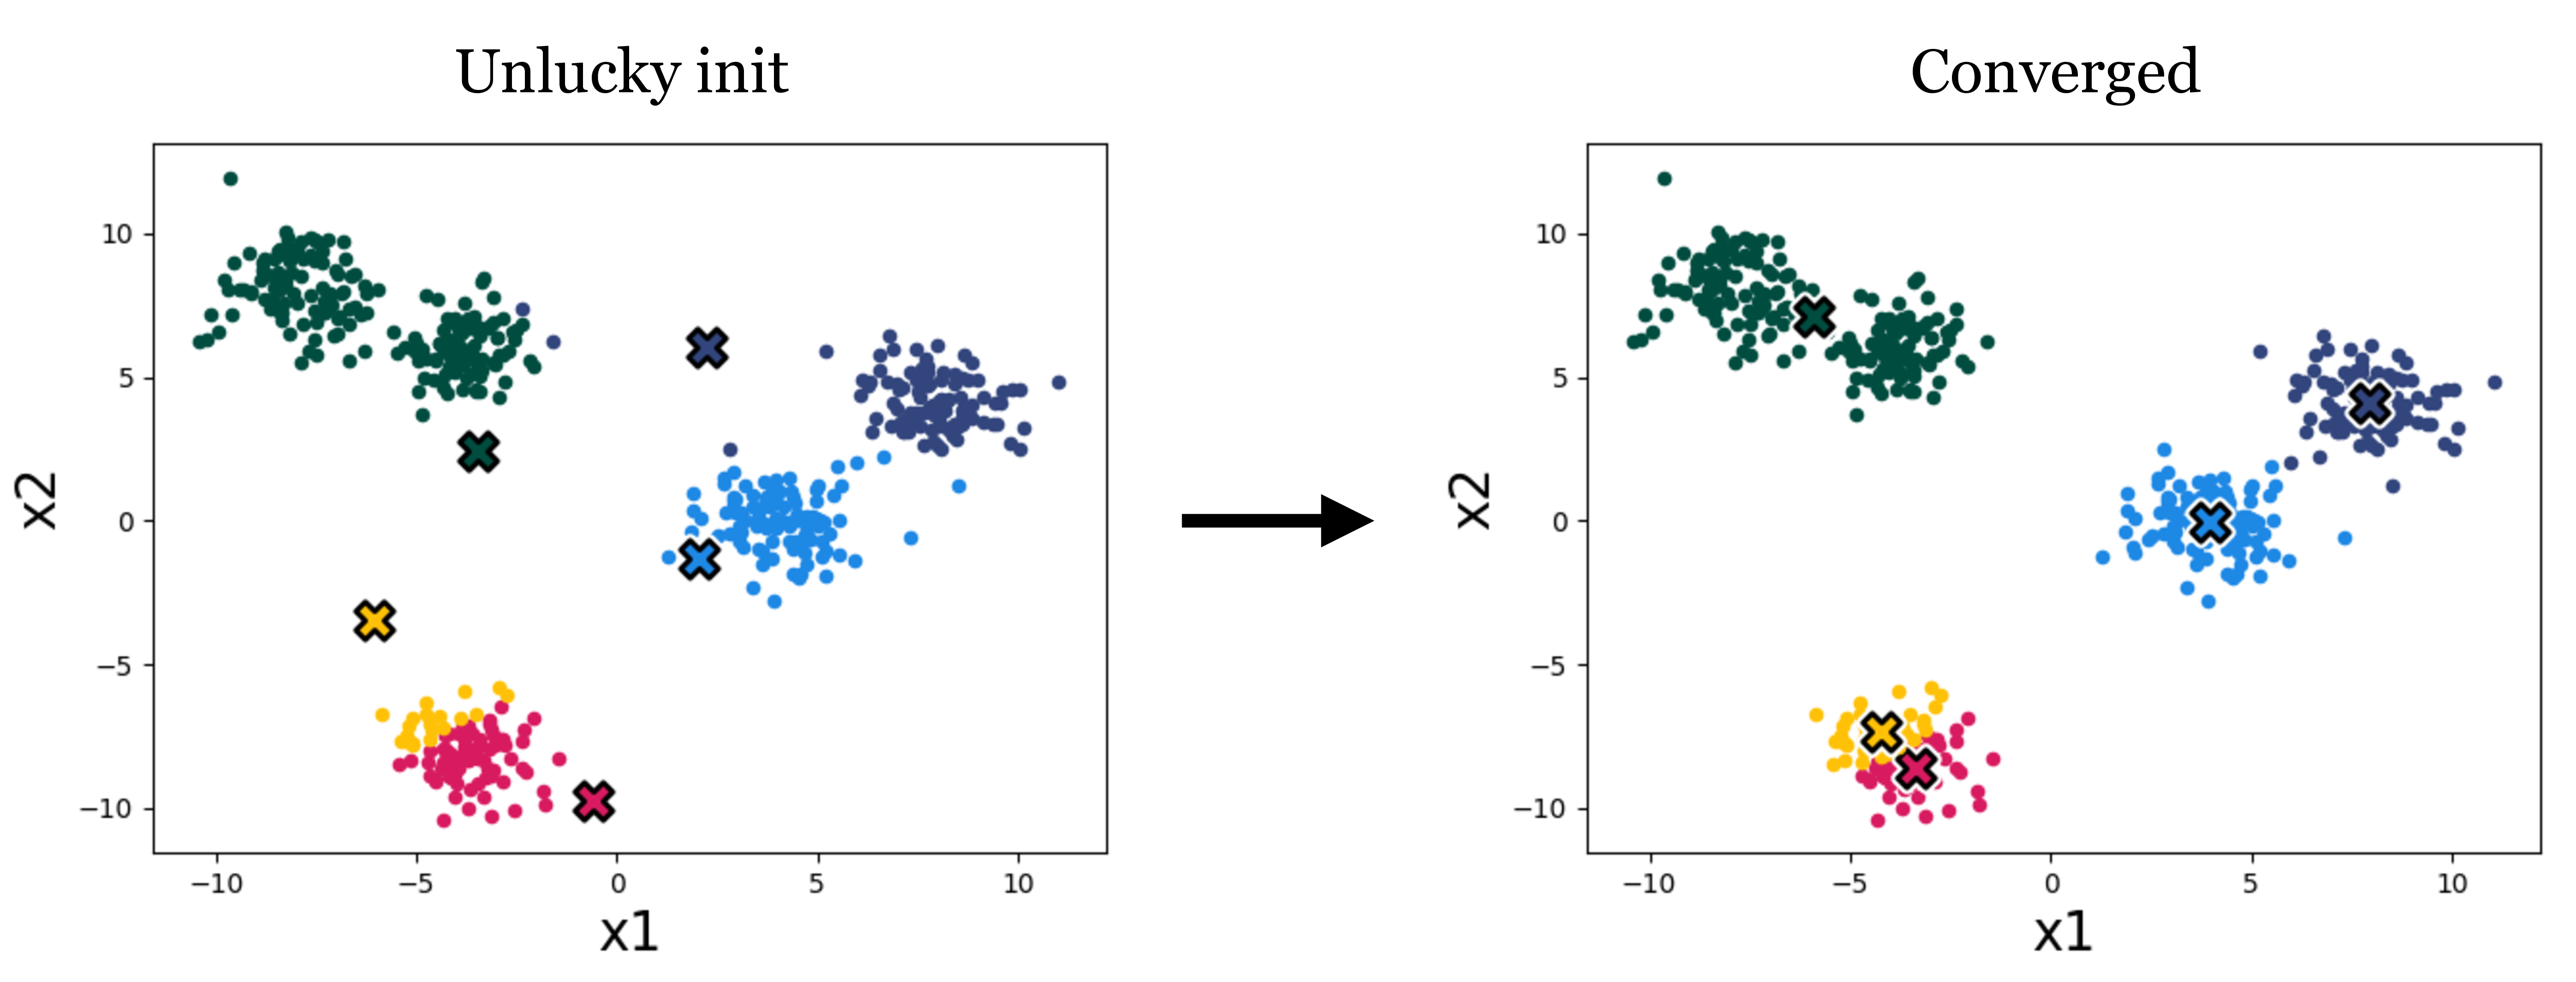
\includegraphics[width=0.8\textwidth]{./figures/kmeans_init.png}
  \caption{With the initialization of the means to the left, the
    yellow and red means end up splitting what perhaps should be one
    cluster in half.}
  \label{fig:kmeans_init}
\end{figure}

A variety of methods have been developed to pick good initializations
(see, for example, the \textit{k-means++} algorithm). One simple
option is to run the standard k-means algorithm multiple times, with
different random initial conditions, and then pick from these the
clustering that achieves the lowest k-means loss.

\subsection{Importance of k}\label{sec-importance_of_k}

A very important parameter in cluster algorithms is the number of
clusters we are looking for. Some advanced algorithms can
automatically infer a suitable number of clusters, but most of the
time, like with k-means, we will have to pick $k$ -- it's a
hyperparameter of the algorithm.

\begin{figure}[h]
  \centering
  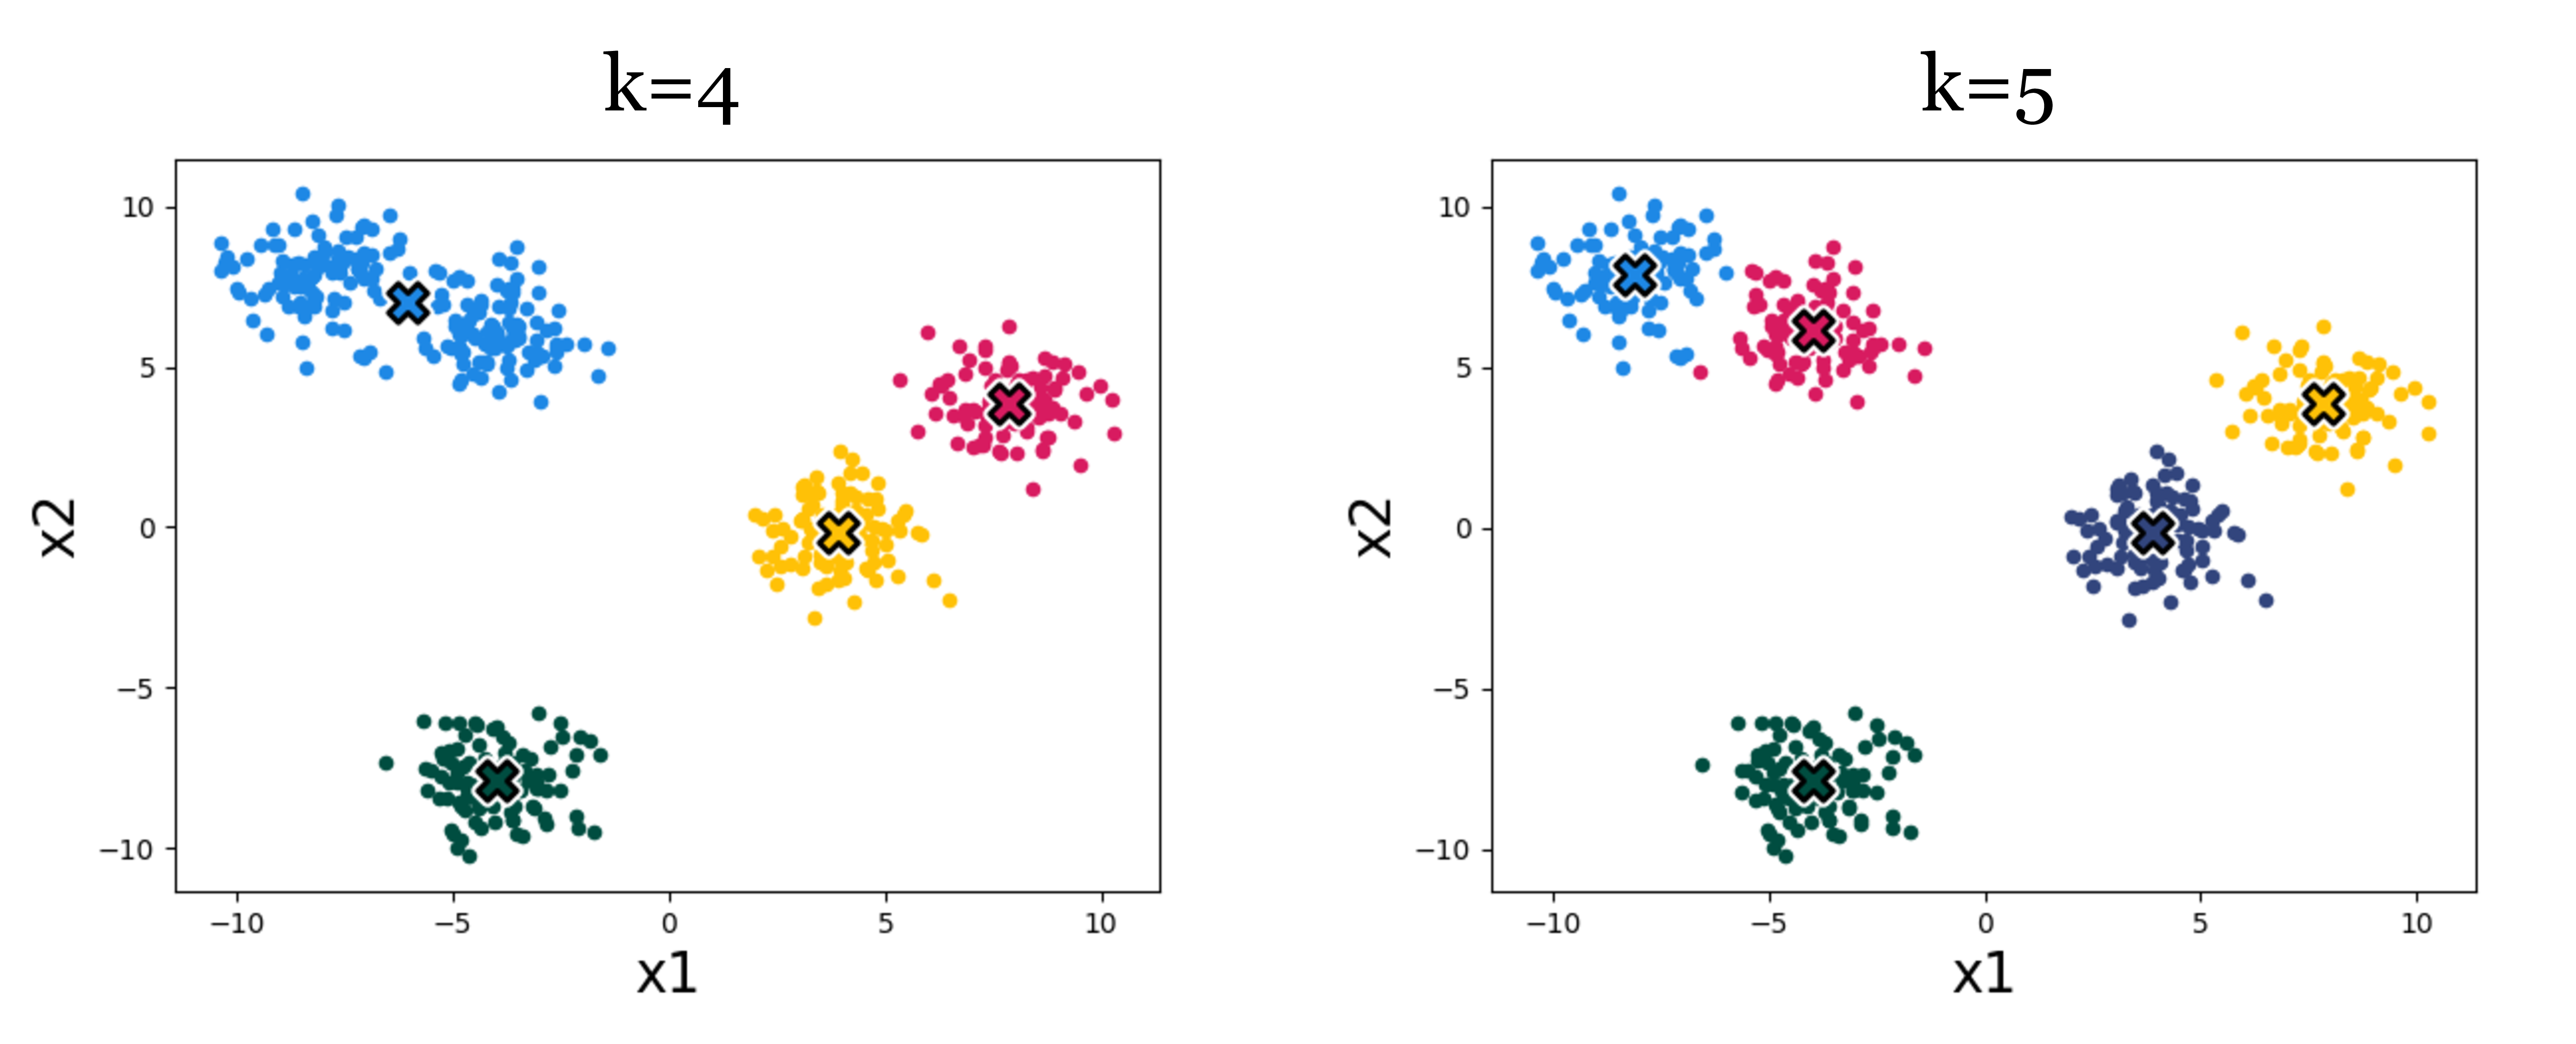
\includegraphics[width=0.67\textwidth]{figures/effect_of_k.png}
  \caption{Example of k-means run on our toy data, with two
    different values of k. Setting k=4, on the left, results in one
    cluster being merged, compared to setting k=5, on the
    right. Which clustering do you think is better? How could you
    decide?}
  \label{fig:effect_of_k}
\end{figure}

Figure~\ref{fig:effect_of_k} shows an example of the effect.  Which
result looks more correct? It can be hard to say! Using higher k we
get more clusters, and with more clusters we can achieve lower
within-cluster variance -- the k-means objective will never increase,
and will typically strictly decrease as we increase k. Eventually, we
can increase k to equal the total number of datapoints, so that each
datapoint is assigned to its own cluster. Then the k-means objective
is zero, but the clustering reveals nothing.  Clearly, then, we cannot
use the k-means objective itself to choose the best value for k. In
Section~\ref{sec-eval}, we will discuss some ways of evaluating the
success of clustering beyond its ability to minimize the k-means
objective, and it's with these sorts of methods that we might decide
on a proper value of k.

Alternatively, you may be wondering: why bother picking a single k?
Wouldn't it be nice to reveal a \textit{hierarchy} of clusterings of
our data, showing both coarse and fine groupings? Indeed
\textit{hierarchical clustering} \index{hierarchical clustering} is another important class of
clustering algorithms, beyond k-means. These methods can be useful for
discovering tree-like structure in data, and they work a bit like this: initially a coarse
split/clustering of the data is applied at the root of the tree, and then as we
descend the tree we split and cluster the data in ever more fine-grained ways. A
prototypical example of hierarchical clustering is to discover a
taxonomy of life, where creatures may be grouped at multiple
granularities, from species to families to kingdoms. You may find a suite of 
clustering algorithms in SKLEARN's 
\href{https://scikit-learn.org/1.5/modules/clustering.html}{cluster} module.


% the
% decision trees we will see later in Chapter~\ref{chap-nonparametric},
% point out: there may be no right answer
%   -- hierarchical call out (different granularities)

% btw there exists a class that finds the whole hierarchy...
% hint at the breadth but focus on k-means

% forge connections to previous topics 
%   -- decision trees and nearest-neighbors
%   -- feature space, autoencoder

\subsection{k-means in feature space}

Clustering algorithms group data based on a notion of
\textit{similarity}, and thus we need to define a \textit{distance metric}
between datapoints. This notion
will also be useful in other machine learning approaches,
such as nearest-neighbor methods that we see in Chapter~\ref{chap-nonparametric}.
In k-means and other methods, our choice of distance
metric can have a big impact on the results we will find.

Our k-means algorithm uses the Euclidean distance, i.e., $\left\Vert
  x^{(i)} - \mu^{(j)} \right\Vert$, with a loss function that is the
square of this distance. We can modify k-means to use different
distance metrics, but a more common trick is to stick with Euclidean
distance but measured in a \textit{feature space}. Just like we did
for regression and classification problems, we can define a feature
map from the data to a nicer feature representation, $\phi(x)$, and
then apply k-means to cluster the data in the\anchorednote{feature
  space.}{In fact, using a simple distance metric in feature space can
  be equivalent to using a more sophisticated distance metric in the
  data space, and this trick forms the basis of \textit{kernel
    methods}, which you can learn about in more advanced machine
  learning classes.}\index{k-means!in feature space}

As a simple example, suppose we have two-dimensional data that is very
stretched out in the first dimension and has less dynamic range in the
second dimension. Then we may want to scale the dimensions so that
each has similar dynamic range, prior to clustering. We could use
standardization, like we did in Chapter~\ref{chap-features}.

If we want to cluster more complex data, like images, music, chemical
compounds, etc., then we will usually need more sophisticated feature
representations. One common practice these days is to use feature
representations learned with a neural network. For example, we can use
an autoencoder to compress images into feature vectors, then cluster
those feature vectors.

%it's best to use a nice feature representation of the data rather
%than the raw format stored on your computer

%As an example, we could use an autoencoder to get the features, as shown here:
% \begin{figure}[h]
%     \centering
%     \includegraphics[width=0.33\textwidth]{example-image-a}
%     \caption{Example of k-means run on some data, in different feature spaces, raw data vs. autoencoder features.}
%     \label{fig:my_label}
% \end{figure}
% connects to week 11's hw too

\section{How to evaluate clustering algorithms}
\label{sec-eval}

\index{clustering!evaluation}
One of the hardest aspects of clustering is knowing how to evaluate
it. This is actually a big issue for all unsupervised learning
methods, since we are just looking for patterns in the data, rather
than explicitly trying to predict target values (which was the case
with supervised learning).

Remember, evaluation metrics are \textit{not} the same as loss
functions, so we can't just measure success by looking at the k-means
loss. In prediction problems, it is critical that the evaluation is on
a held-out test set, while the loss is computed over training data. If
we evaluate on training data we cannot detect overfitting. Something
similar is going on with the example in
Section~\ref{sec-importance_of_k}, where setting k to be too large can
precisely ``fit'' the data (minimize the loss), but yields no general
insight.

One way to evaluate our clusters is to look at the
\textbf{consistency} with which they are found when we run on
different subsamples of our training data, or with different
hyperparameters of our clustering algorithm (e.g.,
initializations). For example, if running on several bootstrapped
samples (random subsets of our data) results in very different
clusters, it should call into question the validity of any of the
individual results.

If we have some notion of what \textbf{ground truth} clusters should
be, e.g., a few data points that we know should be in the same
cluster, then we can measure whether or not our discovered clusters
group these examples correctly.

Clustering is often used for \textbf{visualization} and
\textbf{interpretability}, to make it easier for humans to understand
the data. Here, human judgment may guide the choice of clustering
algorithm. More quantitatively, discovered clusters may be used as input to
\textbf{downstream tasks}. For example, as we saw in the lab, we may fit a different
regression function on the data within each
cluster. Figure~\ref{fig:simpsons_color} gives
an example where this might be useful. In cases like this, the success
of a clustering algorithm can be indirectly measured based on the
success of the downstream application (e.g., does it make the
downstream predictions more accurate).

\begin{figure}[h]
  \centering
  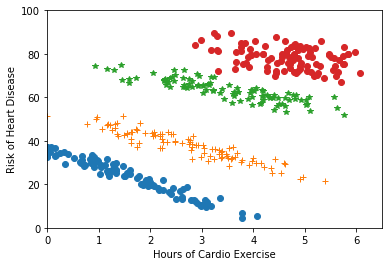
\includegraphics[width=0.35\textwidth]{figures/simpsons_color.png}
  \caption{Averaged across the whole population, risk of heart
    disease positively correlates with hours of exercise. However,
    if we cluster the data, we can observe that there are four
    subgroups of the population which correspond to different age
    groups, and within each subgroup the correlation is negative. We
    can make better predictions, and better capture the presumed
    true effect, if we cluster this data and then model the trend in
    each cluster separately.}
  \label{fig:simpsons_color}
\end{figure}

% Fun stuff to end on?
% High level about unsupervised learning?

% \section{Applications of clustering}

% Clustering has many applications, from visualizing and understanding
% data to efficiently transmitting data over the Internet. Here are a
% few you are now equipped to learn about:

% \begin{itemize}
%     \item ``Vector quantization'' and compression: if we have high-dimensional feature vectors we can summarize them with more compact codewords, i.e., cluster assignments. 
%     \item 
% \end{itemize}

% applications
%  vector quantization; compression

%%% Local Variables:
%%% mode: latex
%%% TeX-master: "top"
%%% End:

% \chapter{Autoencoders}
\label{chap-autoencoders}

In previous chapters, we have largely focused on classification and
regression problems, where we use supervised learning with training
samples that have both features/inputs and corresponding outputs or labels, to
learn hypotheses or models that can then be used to predict labels for
new data.

In contrast to supervised learning paradigm, we can also have an unsupervised learning setting, where we only have features but no
corresponding outputs or labels for our dataset. On natural question aries then: if there are no labels, what are we learning?

%% One canonical example of unsupervised learning is clustering, where
%% the goal is to develop algorithms that can reason about ``similarity''
%% among data points's features, and group the data points into
%% clusters. We will learn about clustering towards the end of the
%% semester in Chapter~\ref{chap-clustering}.

One canonical example of unsupervised learning is clustering,
which we learned about in Chapter~\ref{chap-clustering}.
In clustering, the goal is to develop algorithms that can reason about
``similarity'' among data points's features, and group the data points
into clusters.

  {\em Autoencoders}\index{autoencoder} are another family of unsupervised learning
algorithms, in this case seeking to obtain insights about our data by
learning compressed versions of the original data, or, in other words,
by finding a good lower-dimensional feature representations of the
same data set. Such insights might help us to discover and
characterize underlying factors of variation in data, which can aid in
scientific discovery; to compress data for efficient storage or
communication; or to pre-process our data prior to supervised
learning, perhaps to reduce the amount of data that is needed to learn
a good classifier or regressor.

\section{Autoencoder structure}

Assume that we have input data $\mathcal{D} = \{x^{(1)}, \ldots,
  x^{(n)} \}$, where $x^{(i)}\in \mathbb{R}^d$. We seek to learn an
autoencoder that will output a new dataset $\mathcal{D}_{out} =
  \{a^{(1)}, \ldots, a^{(n)}\}$, where $a^{(i)}\in \mathbb{R}^k$ with $k
  < d$. We can think about $a^{(i)}$ as the new \textit{representation}
of data point $x^{(i)}$. For example, in Fig.~\ref{fig:illustration}
we show the learned representations of a dataset of MNIST digits with
$k=2$. We see, after inspecting the individual data points, that
unsupervised learning has found a compressed (or {\em latent}\index{latent representation})
representation where images of the same digit are close to each
other, potentially greatly aiding subsequent clustering or
classification tasks.

\begin{figure}[h!]
  \centering
  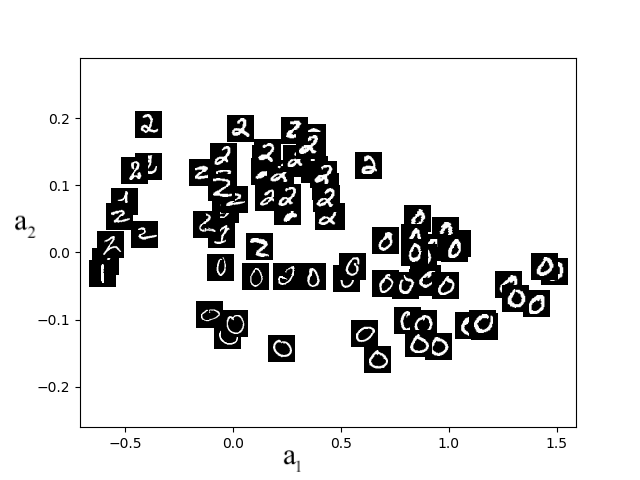
\includegraphics[width= .5\textwidth]{figures/autoencoder_mnist.png}
  \caption{\small Compression of digits dataset into two
    dimensions. The input $x^{(i)}$, an image of a handwritten
    digit, is shown at the new low-dimensional representation
    $(a_1,a_2)$.}
  \label{fig:illustration}
\end{figure}

Formally, an autoencoder consists of two functions, a vector-valued
\textit{encoder} $g : \mathbb{R}^d \rightarrow \mathbb{R}^k$ that
deterministically maps the data to the representation space $a \in
  \mathbb{R}^k$, and a \textit{decoder} $h : \mathbb{R}^k \rightarrow
  \mathbb{R}^d$ that maps the representation space back into the
original data space.

In general, the encoder and decoder functions might be any functions
appropriate to the domain. Here, we are particularly interested in
neural network embodiments of encoders and decoders.
The basic architecture of one such autoencoder, consisting of only a single
layer neural network in each of the encoder and decoder, is shown in
Figure~\ref{fig:autoencoder}; note that bias terms $W^1_0$ and $W^2_0$ into
the summation nodes exist, but are omitted for clarity in the figure.
In this example, the original
$d$-dimensional input is compressed into $k=3$ dimensions via the
encoder $g(x; W^1, W^1_0)=f_1(W{^1}^T x + W^1_0)$ with $W^1 \in
  \mathbb{R}^{d \times k}$ and $W^1_0 \in \mathbb{R}^k$,
and where the non-linearity $f_1$ is applied to each
dimension of the vector. To recover (an approximation to) the
original instance, we then apply the decoder $h(a; W^2, W^2_0) = f_2(W{^2}^T
  a + W^2_0)$, where $f_2$ denotes a different non-linearity (activation
function). In general, both the decoder and the encoder could involve
multiple layers, as opposed to the single layer shown here. Learning
seeks parameters $W^1, W^1_0$ and $W^2, W^2_0$ such that the reconstructed
instances, $h(g(x^{(i)}; W^{1}, W^1_0); W^{2}, W^2_0)$, are close to the original
input $x^{(i)}$.

\begin{figure}[h]
  \centering
  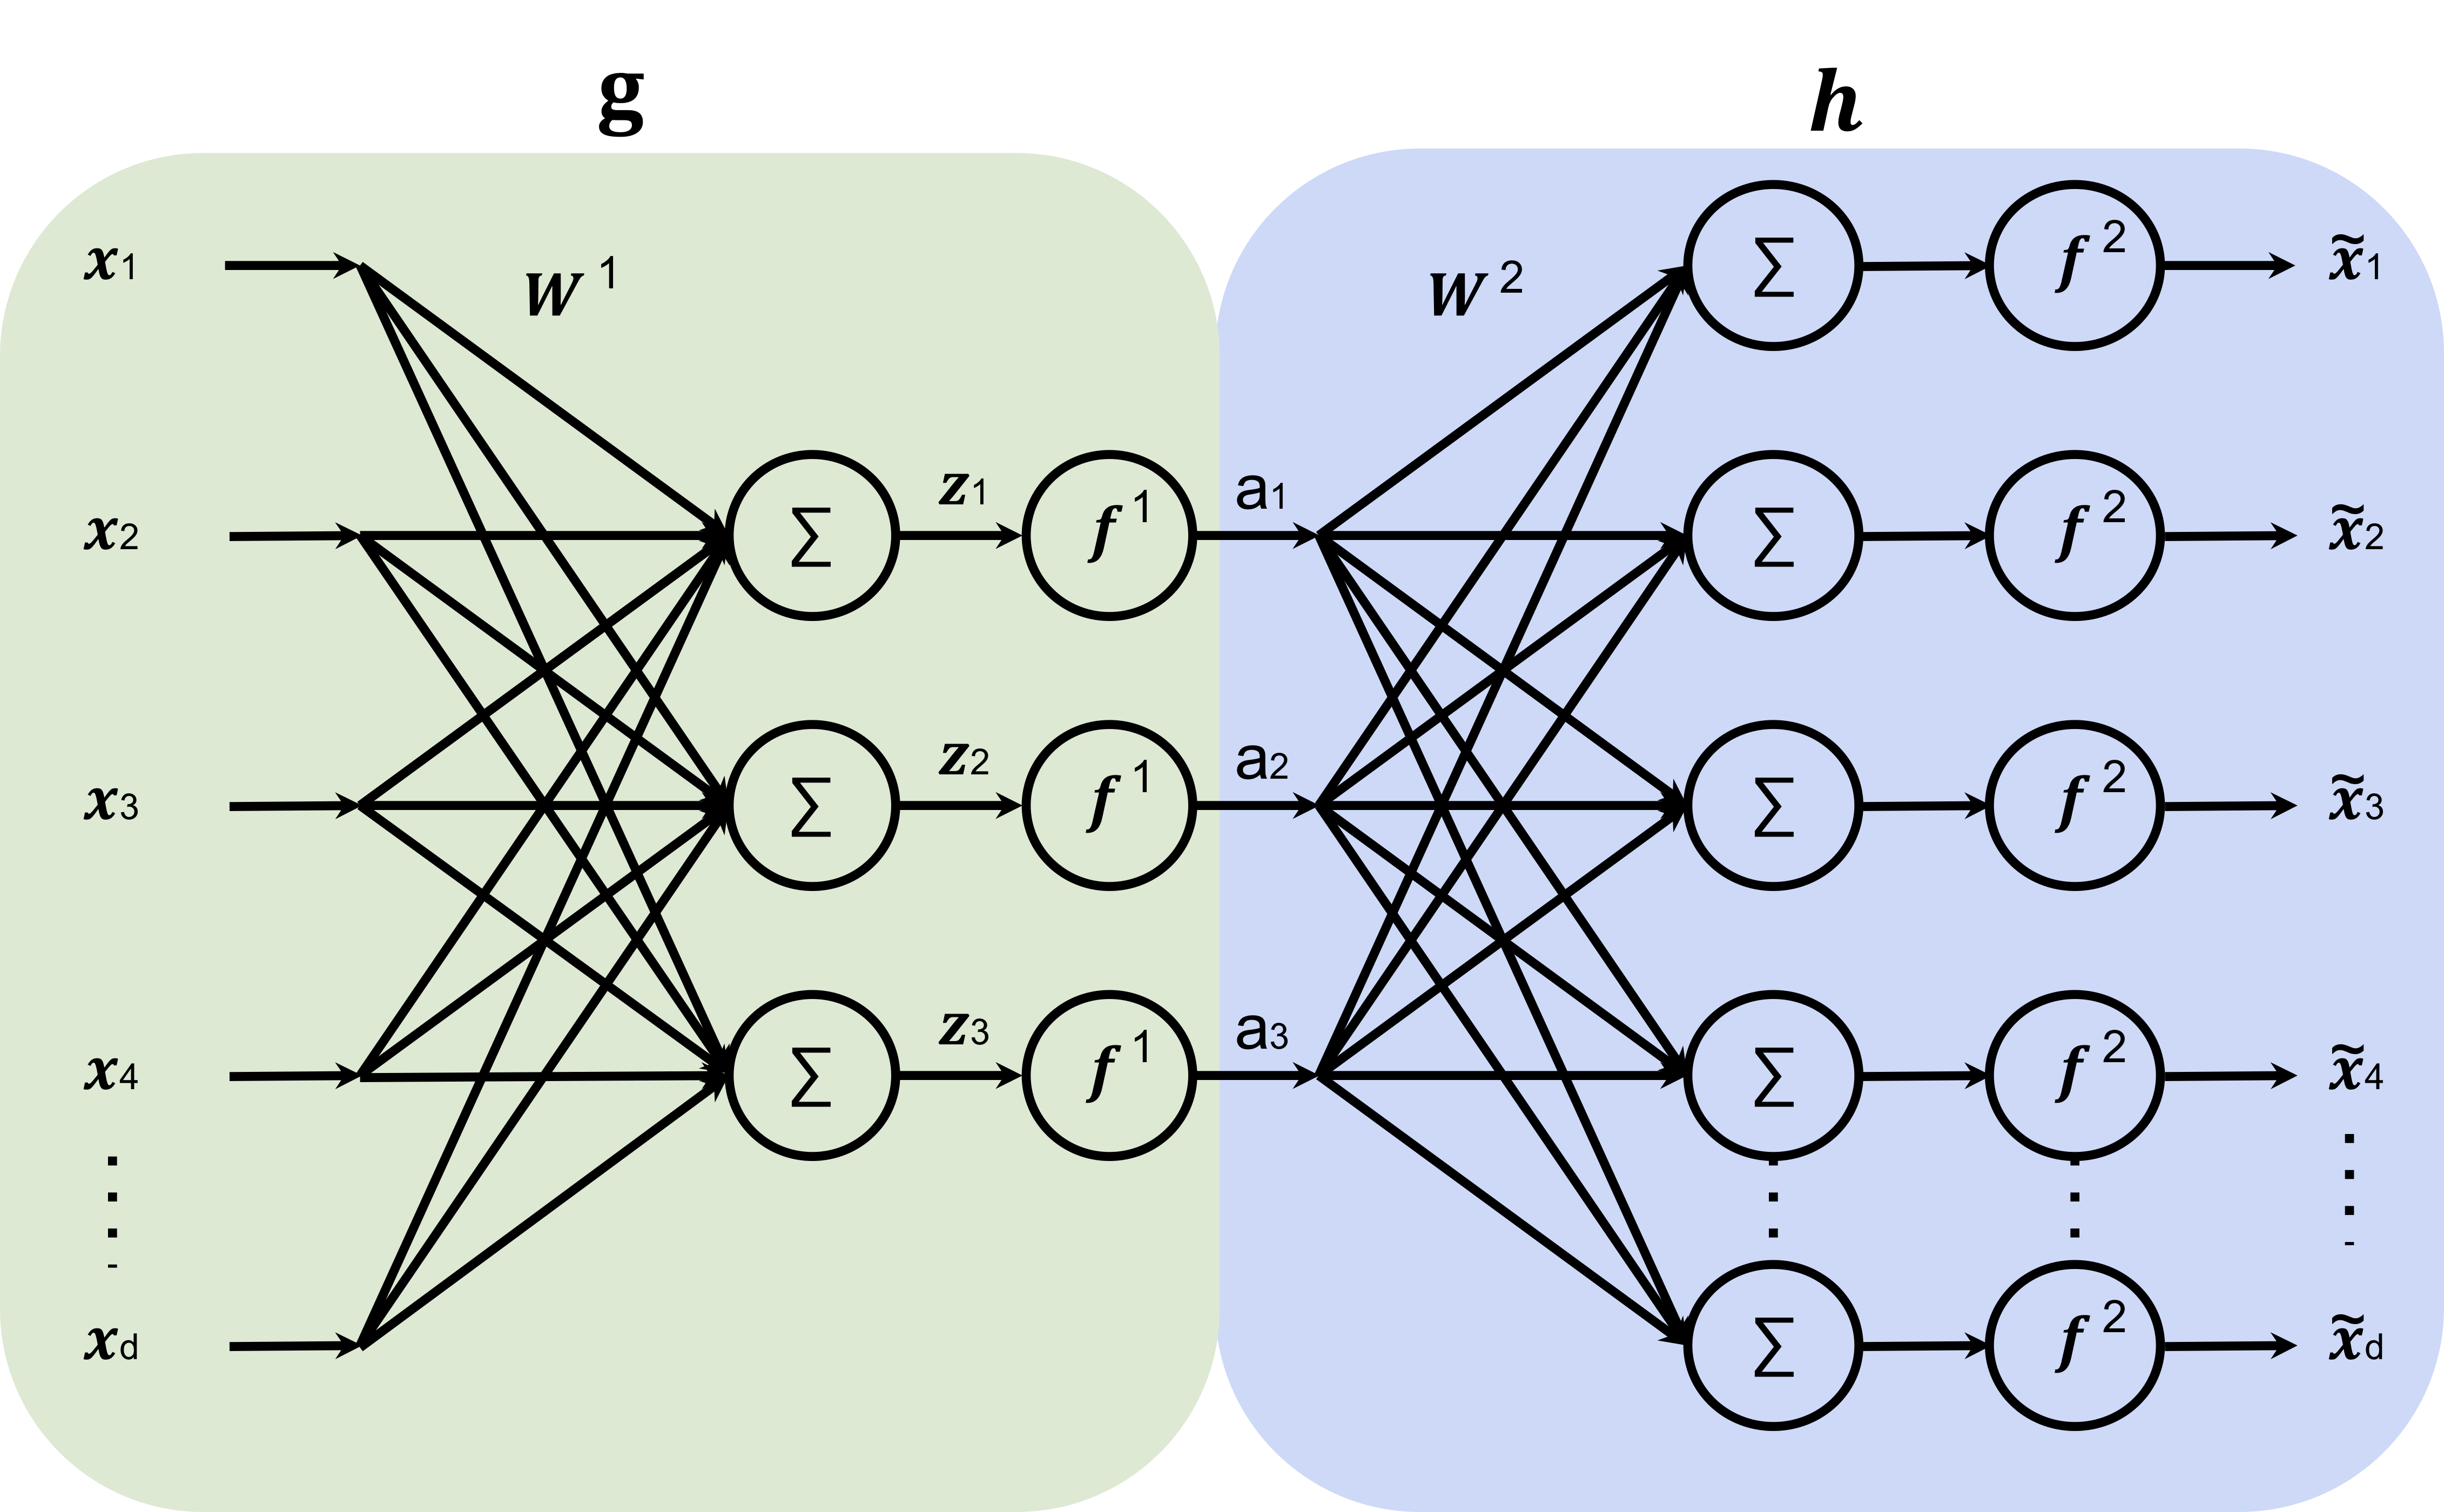
\includegraphics[width= .8\textwidth]{figures/autoencoder.png}
  \caption{\small Autoencoder structure, showing the encoder (left
    half, light green), and the decoder (right half, light blue),
    encoding inputs $x$ to the representation $a$, and decoding the
    representation to produce $\tilde{x}$, the reconstruction.  In
    this specific example, the representation ($a_1$, $a_2$, $a_3$)
    only has three dimensions.\label{fig:autoencoder}}
\end{figure}

\newpage
\section{Autoencoder Learning}

We learn the weights in an autoencoder using the same tools that we previously used for
supervised learning, namely (stochastic) gradient descent of a
multi-layer neural network to minimize a loss function. All that
remains is to specify the loss function $\mathcal{L}(\tilde{x}, x)$, which tells
us how to measure the discrepancy between the reconstruction
$\tilde{x} = h(g(x; W^{1}, W^1_0); W^{2}, W^2_0)$ and the original input $x$. For
example, for continuous-valued $x$ it might make sense to use squared
loss, i.e., $\mathcal{L}_{SE}(\tilde{x}, x) = \sum_{j=1}^{d} (x_j -
  \tilde{x}_j)^2$.\note{Alternatively, you could think of this as {\em
      multi-task learning}, where the goal is to predict each dimension
  of $x$. One can mix-and-match loss functions as appropriate for each
  dimension's data type.} Learning then seeks to optimize the
parameters of $h$ and $g$ so as to minimize the reconstruction error,
measured according to this loss function:
\[
  \min_{W^{1}, W^1_0, W^{2}, W^2_0} \sum_{i=1}^n \mathcal{L}_{SE}\left(h(g(x^{(i)}; W^{1}, W^1_0); W^{2}, W^2_0), x^{(i)}\right)
\]

\section{Evaluating an autoencoder}

What makes a good learned representation in an autoencoder? Notice
that, without further constraints, it is always possible to perfectly
reconstruct the input. For example, we could let $k=d$ and $h$ and $g$
be the identity functions. In this case, we would not obtain any
compression of the data.

To learn something useful, we must create a
\textit{bottleneck} by making $k$ to be smaller (often much smaller)
than $d$. This forces the learning algorithm to seek transformations
that describe the original data using as simple a description as
possible. Thinking back to the digits dataset, for example, an example
of a compressed representation might be the digit label (i.e., 0--9),
rotation, and stroke thickness. Of course, there is no guarantee that
the learning algorithm will discover precisely this
representation. After learning, we can inspect the learned
representations, such as by artificially increasing or decreasing one
of the dimensions (e.g., $a_1$) and seeing how it affects the output
$h(a)$, to try to better understand what it has learned.

As with clustering, autoencoders can be a preliminary step toward
building other models, such as a regressor or classifier. For example,
once a good encoder has been learned, the decoder might be replaced
with another neural network that is then trained with supervised learning
(perhaps using a smaller dataset that does include labels).

\section{Linear encoders and decoders}

We close by mentioning that even linear encoders and decoders can be
very powerful. In this case, rather than minimizing the above
objective with gradient descent, a technique called \textit{principal
  components analysis} (PCA) can be used to obtain a closed-form
solution to the optimization problem using a singular value
decomposition (SVD).  Just as a multilayer neural network with
nonlinear activations for regression (learned by gradient descent) can
be thought of as a nonlinear generalization of a linear regressor (fit
by matrix algebraic operations), the neural network based autoencoders
discussed above (and learned with gradient descent) can be thought of
as a generalization of linear PCA (as solved with matrix algebra by
SVD).

\section{Advanced encoders and decoders}

Advanced neural networks that build on the encoder-decoder conceptual
decomposition have become increasingly powerful in recent years. One
family of applications are {\em generative}\index{generative networks}
networks, where new outputs that are ``similar to'' but different from
any existing training sample are desired. In {\em variational
    autoencoders}\index{autoencoder!variational} the compressed
representation encompasses information about the probability
distribution of training samples, e.g., learning both mean and
standard deviation variables in the bottleneck layer or latent
representation. Then, new outputs can be generated by random sampling
based on the latent representation variables and feeding those samples
into the decoder.

  {\em Transformer} neural networks use {\em multiple} encoder and
decoder blocks, together with a self-attention mechanism to make predictions
about potential next outputs resulting from sequences of inputs. Such
transformer networks have many applications in natural language
processing and elsewhere. We will learn about sequential models in
Chapter~\ref{chap-rnn}.



\begin{appendices}
    \chapter{Matrix derivative common cases}
\label{app:matrix_deriv}

What are some conventions for derivatives of matrices and vectors?  It
will always work to explicitly write all indices and treat everything
as scalars, but we introduce here some shortcuts that are often faster
to use and helpful for understanding.

There are at least two consistent but different systems for describing
shapes and rules for doing matrix derivatives.  In the end, they all
are correct, but it is important to be consistent.

\newcommand{\av}{{\bf a}}
\newcommand{\xv}{{\bf x}}
\newcommand{\yv}{{\bf y}}
\newcommand{\uv}{{\bf u}}
\newcommand{\vv}{{\bf v}}
\newcommand{\fv}{{\bf f}}
\newcommand{\gv}{{\bf g}}
\newcommand{\am}{{\bf A}}
\newcommand{\xm}{{\bf X}}
\newcommand{\ym}{{\bf Y}}

We will use what is often called the `Hessian' or denominator layout,
in which we say that
for

$\xv$ of size $n\times 1$ and $\yv$ of size $m\times 1$,
$\partial \yv/\partial \xv$ is a matrix of size $n\times m$ with the
$(i, j)$ entry $\partial y_j/\partial x_i$.
This denominator layout convention has been adopted by the field of machine
learning to ensure that the shape of the gradient is the same as the shape
of the shape of the respective derivative. This is somewhat controversial at large,
but alas, we shall continue with denominator layout.

The discussion
below closely follows the Wikipedia on matrix derivatives.

\section{The shapes of things}
Here are important special cases of the rule above:

\begin{itemize}

  \item Scalar-by-scalar: For $x$ of size $1\times 1$ and $y$ of size $1\times 1$,
        $\partial y/\partial x$ is the (scalar) partial derivative of $y$
        with respect to $x$.

  \item Scalar-by-vector: For $\xv$ of size $n\times 1$ and $y$ of size $1\times 1$,
        $\partial y/\partial \xv$ (also written $\nabla_\xv y$, the gradient of $y$ with respect to $\xv$)
        is a column vector of size $n\times 1$ with the $i^{\rm th}$ entry $\partial y/\partial
          x_i$:

        \begin{align*}
          \partial y/\partial \xv=
          \begin{bmatrix}
            \partial y/\partial x_1 \\ \partial y/\partial x_2 \\ \vdots \\ \partial y/\partial x_n
          \end{bmatrix}.
        \end{align*}

  \item Vector-by-scalar: For $x$ of size $1\times 1$ and $\yv$ of size $m\times 1$,
        $\partial \yv/\partial x$ is a row vector of size $1 \times m$ with the
        $j^{\rm th}$ entry $\partial \yv_j/\partial x$:

        \begin{align*}
          \partial \yv/\partial x=
          \begin{bmatrix}
            \partial y_1/\partial x & \partial y_2/\partial x & \cdots & \partial y_m/\partial x
          \end{bmatrix}.
        \end{align*}

  \item Vector-by-vector: For $\xv$ of size $n\times 1$ and $\yv$ of size $m\times 1$,
        $\partial \yv/\partial \xv$ is a matrix of size $n\times m$ with the
        $(i, j)$ entry $\partial y_j/\partial x_i$:

        \begin{align*}
          \partial \yv/\partial \xv=
          \begin{bmatrix}
            \partial y_1/\partial x_1 & \partial y_2/\partial x_1 & \cdots & \partial y_m/\partial x_1 \\
            \partial y_1/\partial x_2 & \partial y_2/\partial x_2 & \cdots & \partial y_m/\partial x_2 \\
            \vdots                    & \vdots                    & \ddots & \vdots                    \\
            \partial y_1/\partial x_n & \partial y_2/\partial x_n & \cdots & \partial y_m/\partial x_n \\
          \end{bmatrix}.
        \end{align*}

  \item Scalar-by-matrix: For $\xm$ of size $n\times m$ and $y$ of size $1\times 1$,
        $\partial y/\partial \xm$ (also written $\nabla_\xm y$, the gradient of $y$ with respect to $\xm$)
        is a matrix of size $n\times m$ with the $(i, j)$ entry $\partial y/\partial X_{i, j}$:
        \begin{align*}
          \partial y/\partial \xm=
          \begin{bmatrix}
            \partial y/\partial X_{1,1} & \cdots & \partial y/\partial X_{1,m} \\
            \vdots                      & \ddots & \vdots                      \\
            \partial y/\partial X_{n,1} & \cdots & \partial y/\partial X_{n,m} \\
          \end{bmatrix}.
        \end{align*}

\end{itemize}

You may notice that in this list, we have not included matrix-by-matrix, matrix-by-vector, or vector-by-matrix derivatives.
This is because, generally, they cannot be expressed nicely in matrix form and require higher order objects (e.g., tensors)
to represent their derivatives. These cases are beyond the scope of this course.

Additionally, notice that for all cases, you can explicitly compute each element of the derivative object using (scalar) partial derivatives. You may find it useful to work through some of these by hand as you are reviewing matrix derivatives.


\section{Some vector-by-vector identities}
Here are some examples of $\partial \yv / \partial \xv$.  In each case,
assume $\xv$ is $n \times 1$, $\yv$ is $m \times 1$, $a$ is a scalar
constant, $\av$ is a vector that does not depend on $\xv$ and $\am$ is a matrix that does
not depend on $\xv$, $u$ and $v$ are scalars that do depend on $\xv$, and
$\uv$ and $\vv$ are vectors that do depend on $\xv$.  We also have
vector-valued functions $\fv$ and $\gv$.

\subsection{Some fundamental cases}
First, we will cover a couple of fundamental cases: suppose that $\av$ is an $m \times 1$ vector which is
not a function of $\xv$, an $n\times1$ vector. Then,

\begin{equation}\frac{\partial \av}{\partial \xv} = {\bf 0},
  \label{eq:const}
\end{equation}
is an $n \times m$ matrix of 0s. This is similar to the scalar case of differentiating a constant. Next, we can consider the case of differentiating a vector with respect to itself:

\begin{equation}\frac{\partial \xv}{\partial \xv} = {\bf I}\end{equation}
This is the $n \times n$ identity matrix, with 1's along the
diagonal and 0's elsewhere.  It makes sense, because $\partial \xv_j /
  \xv_i$ is 1 for $i = j$ and 0 otherwise. This identity is also similar to the scalar case.

\subsection{Derivatives involving a constant matrix}

Let the dimensions of $\am$ be $m \times n$. Then the object $\am \xv$ is an $m\times 1$ vector.
We can then compute the derivative of $\am \xv$ with respect to $\xv$ as:

\begin{equation}\frac{\partial \am \xv}{\partial \xv} = \begin{bmatrix}
    \partial (\am \xv)_1/\partial x_1 & \partial (\am \xv)_2/\partial x_1 & \cdots & \partial (\am \xv)_m/\partial x_1 \\
    \partial (\am \xv)_1/\partial x_2 & \partial (\am \xv)_2/\partial x_2 & \cdots & \partial (\am \xv)_m/\partial x_2 \\
    \vdots                            & \vdots                            & \ddots & \vdots                            \\
    \partial (\am \xv)_1/\partial x_n & \partial (\am \xv)_2/\partial x_n & \cdots & \partial (\am \xv)_m/\partial x_n \\
  \end{bmatrix}
\end{equation}

\noindent Note that any element of the column vector $\am \xv$ can be written as, for $j = 1, \ldots, m$:

\[ (\am \xv)_j = \sum_{k=1}^n A_{j,k} x_k.\]

\noindent Thus, computing the $(i,j)$ entry of $\frac{\partial \am \xv}{\partial \xv}$ requires computing the partial derivative $\partial (\am \xv)_j/\partial x_i:$

\begin{align*}
  \partial (\am \xv)_j/\partial x_i = \partial \left( \sum_{k=1}^n A_{j,k} x_k \right)/ \partial x_i = A_{j,i}
\end{align*}

\noindent Therefore, the $(i,j)$ entry of $\frac{\partial \am \xv}{\partial \xv}$ is the $(j,i)$ entry of $\am$:

\begin{equation}
  \frac{\partial \am \xv}{\partial \xv} = \am^T \label{eq:Ax}
\end{equation}

\noindent Similarly, for objects $\xv, \am$ of the same shape, on can obtain,

\begin{equation}
  \frac{\partial \xv^T \am}{\partial \xv} = \am
  \label{eq:xTA}
\end{equation}

\subsection{Linearity of derivatives}

Suppose that $\uv, \vv$ are both vectors of size $m \times 1$. Then,

\begin{equation}
  \frac{\partial (\uv + \vv)}{\partial \xv} = \frac{\partial
    \uv}{\partial \xv} + \frac{\partial \vv}{\partial \xv}
  \label{eq:uplusv}
\end{equation}

\noindent Suppose that $a$ is a scalar constant and $\uv$ is an $m\times 1$ vector that is a function of $\xv$. Then,

\begin{equation}\frac{\partial a \uv}{\partial \xv} = a \frac{\partial \uv}{ \partial \xv}\end{equation}

One can extend the previous identity to vector- and matrix-valued constants. Suppose that $\av$ is a vector with shape $m \times 1$ and $v$ is a scalar which depends on $\xv$. Then,

\begin{equation}\frac{\partial v \av}{\partial \xv} = \frac{\partial
    v}{\partial \xv}\av^T\end{equation}
First, checking dimensions, $\partial v/\partial \xv$ is $n \times
  1$ and $\av$ is $m \times 1$ so $\av^T$ is $1 \times m$ and our
answer is $n \times m$ as it should be.  Now, checking a value,
element $(i,j)$ of the answer is $\partial v \av_j / \partial x_i$ =
$(\partial v / \partial x_i) \av_j$ which corresponds to element
$(i,j)$ of $(\partial v / \partial \xv)\av^T$.

Similarly, suppose that $\am$ is a matrix which does not depend on $\xv$ and $\uv$ is a column vector which does depend on $\xv$. Then,

\begin{equation}\frac{\partial \am \uv}{\partial \xv} = \frac{\partial
    \uv}{\partial \xv}\am^T\end{equation}

\subsection{Product rule (vector-valued numerator)}

Suppose that $v$ is a scalar which depends on $\xv$, while $\uv$ is a column vector of shape $m\times 1$ and $\xv$ is a column vector of shape $n \times 1$. Then,

\begin{equation}\frac{\partial v \uv}{\partial \xv} = v\frac{\partial
    \uv}{\partial \xv} + \frac{\partial v}{\partial \xv} \uv^T\end{equation}

One can see this relationship by expanding the derivative as follows:

\begin{align*}
  \frac{\partial v \uv}{\partial \xv} =
  \begin{bmatrix}
    \partial (v u_1)/\partial x_1 & \partial (v u_2)/\partial x_1 & \cdots & \partial (v u_m)/\partial x_1 \\
    \partial (v u_1)/\partial x_2 & \partial (v u_2)/\partial x_2 & \cdots & \partial (v u_m)/\partial x_2 \\
    \vdots                        & \vdots                        & \ddots & \vdots                        \\
    \partial (v u_1)/\partial x_n & \partial (v u_2)/\partial x_n & \cdots & \partial (v u_m)/\partial x_n \\
  \end{bmatrix}.
\end{align*}

Then, one can use the product rule for scalar-valued functions,
\begin{align*}
  \partial (v u_j)/\partial x_i = v (\partial u_j / \partial x_i) + (\partial v / \partial x_i) u_j,
\end{align*}
to obtain the desired result.

\subsection{Chain rule}
Suppose that $\gv$ is a vector-valued function with output vector of shape $m \times 1$, and the argument to $\gv$ is a column vector $\uv$ of shape $d\times 1$ which depends on $\xv$. Then, one can obtain the chain rule as,

\begin{equation}\frac{\partial \gv(\uv)}{\partial \xv} = \frac{\partial
    \uv}{\partial \xv}\frac{\partial \gv(\uv)}{\partial
    \uv}\end{equation}
Following ``the shapes of things,''
$\partial \uv / \partial \xv$ is $n \times d$ and $\partial \gv(\uv)
  / \partial \uv$ is $d \times m$, where element $(i,j)$ is $\partial
  \gv(\uv)_j / \partial \uv_i$.
The same chain rule applies for further compositions of functions:
\begin{equation}\frac{\partial \fv(\gv(\uv))}{\partial \xv} = \frac{\partial
    \uv}{\partial \xv}\frac{\partial \gv(\uv)}{\partial \uv}
  \frac{\partial \fv(\gv)}{\partial \gv}\end{equation}


\section{Some other identities}
You can get many scalar-by-vector and vector-by-scalar cases as special
cases of the rules above, making one of the relevant vectors just be
1 x 1.  Here are some other ones that are handy.  For more, see the
Wikipedia article on Matrix derivatives (for consistency, only use
the ones in {\em denominator layout}).

\begin{equation}
  \frac{\partial \uv^T \vv}{\partial \xv} = \frac{\partial
    \uv}{\partial \xv} \vv + \frac{\partial \vv}{\partial \xv} \uv
  \label{eq:uTv}
\end{equation}

\begin{equation}
  \frac{\partial \uv^T}{\partial x} = \big(\frac{\partial
    \uv}{\partial x}\big)^T
  \label{eq:uT}
\end{equation}



\section{Derivation of gradient for linear regression}
\label{app:matrix-gradient}

\newcommand{\xmt}{\tilde{\bf X}}
\newcommand{\ymt}{\tilde{\bf Y}}


Applying identities \ref{eq:xTA}, \ref{eq:uTv}, \ref{eq:uplusv}, \ref{eq:Ax}
\ref{eq:const}
\begin{align*}
  \frac{\partial (\xmt \theta - \ymt)^T(\xmt \theta - \ymt)/n}{\partial
  \theta} & = \frac{2}{n} \frac{\partial(\xmt \theta - \ymt)}{\partial
  \theta}(\xmt \theta - \ymt)                                           \\
          & = \frac{2}{n} \big(\frac{\partial\xmt \theta}{\partial
    \theta}-\frac{\partial \ymt}{\partial
  \theta}\big)(\xmt \theta - \ymt)                                      \\
          & = \frac{2}{n} \big(\xmt^T -{\bf 0}\big)(\xmt \theta - \ymt) \\
          & = \frac{2}{n} \xmt^T (\xmt \theta - \ymt)                   \\
\end{align*}


\section{Matrix derivatives using Einstein summation}
\label{app:einstein}

{\em You do not have to read or learn this!  But you might find it
  interesting or helpful.}

\def\bea{\begin{eqnarray}}
    \def\eea{\end{eqnarray}}
\def\Xt{\tilde{X}}
\def\Yt{\tilde{Y}}

Consider the objective function for linear regression, written out as products of matrices:
\bea
J(\theta) = \frac{1}{n} (\Xt\theta - \Yt)^T (\Xt\theta-\Yt)
\,,
\eea
where $\Xt = X^T$ is $n\times d$, $\Yt=Y^T$ is $n\times 1$, and $\theta$ is $d\times 1$.  How does one show, with no shortcuts, that
\bea
\nabla_{\theta}J = \frac{2}{n} {\Xt^T} {(\Xt\theta - \Yt)} \;\;?
\eea
One neat way, which is very explicit, is to simply write all the
matrices as variables with row and column indices, e.g., $\Xt_{ab}$ is
the row $a$, column $b$ entry of the matrix $\Xt$.  Furthermore, let
us use the convention that in any product, all indices which appear
more than once get summed over; this is a popular convention in
theoretical physics, and lets us suppress all the summation symbols
which would otherwise clutter the following expresssions.  For
example, $\Xt_{ab} \theta_b$ would be the implicit summation notation
giving the element at the $a^{\rm th}$ row of the matrix-vector
product $\Xt \theta$.

Using implicit summation notation with explicit indices,
we can rewrite $J(\theta)$ as
\bea
J(\theta) = \frac{1}{n} \left( \Xt_{ab} \theta_b - \Yt_a \right)  \left( \Xt_{ac}\theta_c - \Yt_a \right) \,.
\eea
Note that we no longer need the transpose on the first term, because
all that transpose accomplished was to take a dot product between the
vector given by the left term, and the vector given by the right term.
With implicit summation, this is accomplished by the two terms sharing
the repeated index $a$.

Taking the derivative of $J$ with respect to the $d^{\rm th}$ element
of $\theta$ thus gives, using the chain rule for (ordinary scalar)
multiplication:
\bea
\frac{dJ}{d\theta_d} &=& \frac{1}{n} \left[
  \Xt_{ab} \delta_{bd} \left( \Xt_{ac}\theta_c-\Yt_a \right)
  + \left(\Xt_{ab}\theta_b - \Yt_a \right) \Xt_{ac} \delta_{cd}
  \right]
\\
&=& \frac{1}{n} \left[
  \Xt_{ad} \left( \Xt_{ac}\theta_c-\Yt_a \right)
  + \left(\Xt_{ab}\theta_b - \Yt_a \right) \Xt_{ad}
  \right]
\\
&=& \frac{2}{n} \Xt_{ad} \left( \Xt_{ab}\theta_b-\Yt_a \right)
\,,
\eea
where the second line follows from the first, with the definition that
$\delta_{bd} = 1$ only when $b=d$ (and similarly for $\delta_{cd}$).
And the third line follows from the second by recognizing that the two
terms in the second line are identical.  Now note that in this
implicit summation notation, the $a, b$ element of the matrix product
of $A$ and $B$ is $(AB)_{ac} = A_{ab}B_{bc}$.  That is, ordinary
matrix multiplication sums over indices which are adjacent to each
other, because a row of $A$ times a column of $B$ becomes a scalar
number.  So the term in the above equation with $\Xt_{ad} \Xt_{ab}$ is
not a matrix product of $\Xt$ with $\Xt$.  However, taking the
transpose $\Xt^T$ switches row and column indices, so $\Xt_{ad} = \Xt^T_{da}$.
And $\Xt^T_{da} \Xt_{ab}$ {\em is} a matrix product of $\Xt^T$ with $\Xt$!
Thus, we have that
\bea
\frac{dJ}{d\theta_d} &=& \frac{2}{n} \Xt^T_{da} \left( \Xt_{ab}\theta_b-\Yt_a \right)
\\
&=& \frac{2}{n} \left[ \Xt^T \left( \Xt\theta-\Yt \right) \right]_{d}
\,,
\eea
which is the desired result.

%%% Local Variables:
%%% mode: latex
%%% TeX-master: "top"
%%% End:

    \chapter{Optimizing Neural Networks}
\label{sec-nn-details}

\subsection{Strategies towards adaptive step-size}\label{adaptive-step-size-appendix}
\subsubsection{Running averages}
\index{adaptive step size!running average}
We'll start by looking at the notion of a {\em running average}.  It's
a computational strategy for estimating a possibly weighted average of
a sequence  of data.  Let our data sequence be $c_1, c_2, \ldots$;
then we define a sequence of running average values, $C_0, C_1, C_2,
  \ldots$ using the equations
\begin{align*}
  C_0 & = 0                                       \\
  C_t & =  \gamma_t C_{t-1} +  (1 - \gamma_t) c_t
\end{align*}
where $\gamma_t \in (0, 1)$.  If $\gamma_t$ is a constant, then this
is a {\em  moving} average, in which
\begin{align*}
  C_T & = \gamma C_{T-1} + (1  - \gamma) c_T                                  \\
      & = \gamma (\gamma C_{T-2} + (1  - \gamma) c_{T-1}) + (1  - \gamma) c_T \\
      & = \sum_{t = 1}^T \gamma^{T-t}(1 - \gamma) c_t
\end{align*}
So, you can see that inputs $c_t$ closer to the end of the sequence $T$
have  more effect on $C_T$ than early inputs.

If, instead, we set $\gamma_t = (t - 1)  / t$, then we get the actual
average.
\question{
  Prove to yourself that the previous assertion holds.
}
% \begin{align*}
% A_1 &= a_1\\
% A_2 &= \frac{1}{2}A_1 + \frac{1}{2}a_2 = \frac{1}{2}(a_1 + a_2)\\
% A_3 &= \frac{2}{3}A_2 + \frac{1}{3}a_3 = \frac{2}{3} \cdot \frac{1}{2}(a_1 + a_2) + \frac{1}{3}a_3 = \frac{1}{3}(a_1 + a_2 + a_3)
% \end{align*}

\subsubsection{Momentum} \index{adaptive step size!momentum}
Now, we can use methods that are a bit like running averages to
describe strategies for computing $\eta$.
The simplest method is {\em momentum}, in  which we try to ``average'' recent
gradient updates,  so that if they have been bouncing back and forth
in some direction, we take out that component of the motion.  For
momentum, we have
\begin{align*}
  V_0 & = 0                                         \\
  V_t & = \gamma V_{t-1} + \eta \nabla_W J(W_{t-1}) \\
  W_t & = W_{t-1} - V_t
\end{align*}
This doesn't quite look like an adaptive step size.  But what we can
see is that, if we let $\eta = \eta'(1 - \gamma)$, then the rule looks exactly like doing an update with
step size $\eta'$ on a moving average of the gradients with parameter
$\gamma$:
\begin{align*}
  M_0 & = 0                                                 \\
  M_t & = \gamma M_{t-1} + (1 - \gamma) \nabla_W J(W_{t-1}) \\
  W_t & = W_{t-1} - \eta' M_t
\end{align*}
\question{Prove to yourself that these formulations are equivalent.}


We will find that $V_t$ will be bigger in dimensions that consistently
have the same sign for $\nabla_{W}$ and smaller for those that
don't.   Of course we now have {\em two}  parameters  to set ($\eta$
and $\gamma$), but the
hope is  that the algorithm will perform better overall, so it will be
worth trying to find good values for them.  Often $\gamma$ is  set to
be something like $0.9$.
\begin{examplebox}
  \begin{center}
    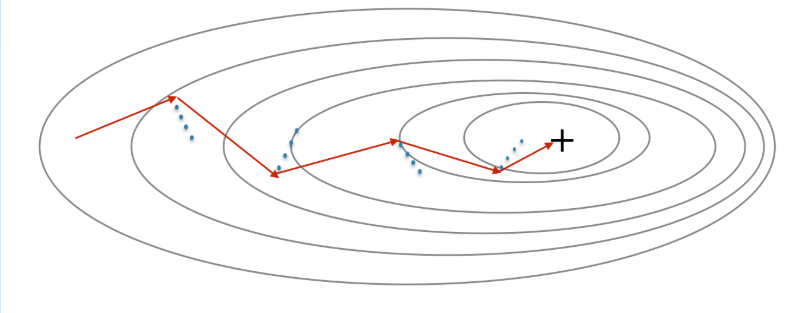
\includegraphics[scale=0.7]{figures/momentum.png}
  \end{center}
  The red arrows show the update after each successive step of
  mini-batch gradient descent with momentum.  The blue points show the
  direction of the gradient with respect to the mini-batch at each step.
  Momentum smooths the path taken towards the local minimum and leads to
  faster convergence.
\end{examplebox}
\question{If you set $\gamma = 0.1$, would momentum have more of an
  effect or less of an effect than if you set it to $0.9$?
}

\subsubsection{Adadelta}\index{adaptive step size!adadelta}
Another useful idea is this:  we would like to take larger steps in
parts of the space where $J(W)$ is nearly flat (because there's no risk of
taking too big a step due to the gradient being large) and smaller
steps when it is steep.  We'll apply this idea to each weight
independently, and end up with a method called {\em adadelta}, which
is a variant on {\em adagrad} (for
adaptive gradient).   Even though our weights are indexed by layer,
input unit and output unit,  for simplicity here,  just let $W_j$ be
any weight in the network (we will do the same thing for all of
them).
\begin{align*}
  g_{t,j} & = \nabla_W J(W_{t-1})_j                                      \\
  G_{t,j} & = \gamma G_{t - 1,j} + (1 - \gamma)g_{t,j}^2                 \\
  W_{t,j} & = W_{t-1, j} - \frac{\eta}{\sqrt{G_{t,j} + \epsilon}}g_{t,j}
\end{align*}
The sequence $G_{t,j}$ is a moving average of the  square of the
$j$th component of the gradient.  We square it in order to be
insensitive to the sign---we want to know whether the magnitude is big
or small.  Then, we perform a gradient update to weight $j$, but
divide the step  size by $\sqrt{G_{t,j} + \epsilon}$, which is larger
when the surface is steeper in direction $j$ at point $W_{t-1}$ in
weight space;  this means that the step size will be smaller when it's
steep and  larger when it's flat.

\subsubsection{Adam}\index{adaptive step size!adam}

Adam has become the default method of managing step sizes in neural
networks\note{Although,  interestingly, it may actually violate the
convergence conditions of {\sc sgd}: {\scriptsize\tt
arxiv.org/abs/1705.08292}}.   It combines the ideas  of
momentum and adadelta.  We start by writing moving averages of the
gradient and squared gradient, which reflect estimates of the mean and
variance of the gradient for weight $j$:
\begin{align*}
  g_{t,j} & = \nabla_W J(W_{t-1})_j                      \\
  m_{t,j} & = B_1m_{t - 1,j} + (1 - B_1)g_{t,j}          \\
  v_{t,j} & = B_2v_{t - 1,j} + (1 - B_2)g_{t,j}^2  \;\;.
\end{align*}

A problem with these estimates is that, if we initialize $m_0 = v_0 = 0$,
they will always be biased (slightly too small).  So we will correct
for that bias  by defining
\begin{align*}
  \hat{m}_{t,j} & = \frac{m_{t,j}}{1 - B^t_1}                     \\
  \hat{v}_{t,j} & = \frac{v_{t,j}}{1 - B^t_2}                     \\
  W_{t,j}       & = W_{t-1,j} - \frac{\eta}{\sqrt{\hat{v}_{t,j} +
      \epsilon}}\hat{m}_{t,j} \;\;.
\end{align*}
Note that $B^t_1$ is $B_1$ raised to the power $t$, and likewise for
$B^t_2$.  To justify these corrections, note that if we were to expand $m_{t,j}$
in terms of $m_{0,j}$ and $g_{0,j}, g_{1,j}, \dots, g_{t,j}$ the coefficients would
sum to $1$.  However, the coefficient behind $m_{0,j}$ is $B_1^t$ and since
$m_{0,j} = 0$, the sum of coefficients of non-zero terms is $1 - B_1^t$, hence
the correction.  The same justification holds for $v_{t,j}$.

Now, our update for weight $j$ has a step size that takes the
steepness into account, as in adadelta, but also tends to move in the
same direction, as in momentum.  The authors of this method propose
setting $B_1 = 0.9, B_2 = 0.999, \epsilon = 10^{-8}$.  Although we now
have even more parameters, Adam is not highly sensitive to their values
(small changes do not have a huge effect on the result).
\question{Define $\hat{m_j}$ directly as a moving average of
  $g_{t,j}$.  What is the decay ($\gamma$ parameter)?
}
Even though we now have a step-size for each weight, and we have to
update various quantities on each iteration of gradient descent, it's
relatively easy to implement by maintaining a matrix for each quantity
($ m^{\ell}_t, v^{\ell}_t, g^{\ell}_t, {g^{2}_t}^{\ell} $) in each
layer of the network.





% 

\subsection{Batch Normalization Details}\label{batch-norm-appendix}

Let's think of the batch-norm layer as taking $Z^l$ as input and
producing an output $\widehat{Z}^l$ as output.  But now, instead of
thinking of $Z^l$ as an $n^l \times 1$ vector, we have to explicitly
think about handling a mini-batch of data of size $K$, all at once, so
$Z^l$ will be $n^l \times K$, and so will the output $\widehat{Z}^l$.

Our first step will be to compute the {\em batchwise} mean and
standard deviation.  Let $\mu^l$ be the $n^l \times 1$ vector where
\[\mu^l_i = \frac{1}{K} \sum_{j = 1}^K Z^l_{ij}\;\;,\]
and let $\sigma^l$ be the $n^l \times 1$ vector where
\[\sigma^l_i = \sqrt{\frac{1}{K} \sum_{j = 1}^K (Z^l_{ij} - \mu_i)^2}\;\;.\]

The basic normalized version of our data would be a matrix,
element $(i, j)$ of which is
\[\overline{Z}^l_{ij} = \frac{Z^l_{ij} - \mu^l_i}{\sigma^l_i + \epsilon}\;\;,\]
where $\epsilon$ is a very small constant to guard against division by
zero.
However, if we let these be our $\widehat{Z}^l$ values, we really are
forcing something too strong on our data---our goal was to normalize
across the data batch, but not necessarily force the output values to
have exactly mean 0 and standard deviation 1.  So, we will give the
layer the ``opportunity'' to shift and scale the outputs by adding new
weights to the layer.  These weights are $G^l$ and $B^l$, each of
which is an $n^l \times 1$ vector.  Using the weights, we define the
final output to be
\[\widehat{Z}^l_{ij} = G^l_i \overline{Z}^l_{ij} + B^l_i\;\;.\]
That's the forward pass.  Whew!

Now, for the backward pass, we have to do two things:  given
$\partial L / \partial \widehat{Z}^l$,
\begin{itemize}
  \item Compute $\partial L / \partial Z^l$ for back-propagation, and
  \item Compute $\partial L / \partial G^l$ and $\partial L / \partial
          B^l$ for gradient updates of the weights in this layer.
\end{itemize}

Schematically\note{For simplicity we will drop the reference to the layer $l$ in the rest of the derivation}
\[\frac{\partial L}{\partial B} = \frac{\partial L}{\partial
    \widehat{Z}}\frac{\partial \widehat{Z}}{\partial B}\;\;.\]
It's hard to think about these derivatives in matrix terms, so we'll
see how it works for the components.
$B_i$ contributes to $\widehat{Z}_{ij}$ for all data points $j$ in the
batch.  So
\begin{align*}
  \frac{\partial L}{\partial B_i} & =
  \sum_j \frac{\partial L}{\partial \widehat{Z}_{ij}}
  \frac{\partial \widehat{Z}_{ij}}{\partial B_i}                                               \\
                                  & = \sum_j \frac{\partial L}{\partial \widehat{Z}_{ij}}\;\;,
\end{align*}
Similarly, $G_i$ contributes to $\widehat{Z}_{ij}$ for all data points
$j$ in the batch.  So
\begin{align*}
  \frac{\partial L}{\partial G_i} & =
  \sum_j \frac{\partial L}{\partial \widehat{Z}_{ij}}
  \frac{\partial \widehat{Z}_{ij}}{\partial G_i}                                                                  \\
                                  & =  \sum_j \frac{\partial L}{\partial \widehat{Z}_{ij}} \overline{Z}_{ij}\;\;.
\end{align*}
Now, let's figure out how to do backprop.  We can start schematically:
\[\frac{\partial L}{\partial Z} = \frac{\partial L}{\partial \widehat{Z}}
  \frac{\partial \widehat{Z}}{\partial Z}\;\;.\]
And because dependencies only exist across the batch, but not across
the unit outputs,
\[\frac{\partial L}{\partial Z_{ij}} =
  \sum_{k=1}^K\frac{\partial L}{\partial \widehat{Z}_{ik}}
  \frac{\partial \widehat{Z}_{ik}}{\partial Z_{ij}}\;\;.\]
The next step is to note that
\begin{align*}
  \frac{\partial \widehat{Z}_{ik}}{\partial Z_{ij}} & =
  \frac{\partial \widehat{Z}_{ik}}{\partial \overline{Z}_{ik}}
  \frac{\partial \overline{Z}_{ik}}{\partial Z_{ij}}                                                                \\
                                                    & = G_i \frac{\partial \overline{Z}_{ik}}{\partial Z_{ij}}\;\;.
\end{align*}
And now that
\[
  \frac{\partial \overline{Z}_{ik}}{\partial Z_{ij}}  =
  \left(\delta_{jk} - \frac{\partial \mu_i}{\partial Z_{ij}}\right) \frac{1}{\sigma_i} -
  \frac{Z_{ik} - \mu_i}{\sigma_i^2} \frac{\partial \sigma_i}{\partial Z_{ij}} \;\;,
\]
where $\delta_{jk} = 1$ if $j = k$ and $\delta_{jk} = 0$ otherwise.
Getting close!  We need two more small parts:
\begin{align*}
  \frac{\partial \mu_i}{\partial Z_{ij}}    & = \frac{1}{K} \;, \\
  \frac{\partial \sigma_i}{\partial Z_{ij}} & =
  \frac{Z_{ij} - \mu_i}{K \sigma_i}\;\;.
\end{align*}
Putting the whole crazy thing together, we get
\[\frac{\partial L}{\partial Z_{ij}} =
  \sum_{k=1}^K\frac{\partial L}{\partial \widehat{Z}_{ik}}
  G_i\frac{1}{K \sigma_i}\left(\delta_{jk}K-1 - \frac{(Z_{ik} - \mu_i)(Z_{ij} - \mu_i)}{\sigma_i^2}
  \right)\;\;.
\]
    %% Thanks to Ike for this!



%%% Local Variables:
%%% mode: latex
%%% TeX-master: "top"
%%% End:

    \chapter{Recurrent Neural Networks}
\label{chap-rnn}

So far, we have limited our attention to domains in which each output
$y$ is assumed to have been generated as a function of an associated
input $x$, and our hypotheses have been ``pure'' functions, in which
the output depends only on the input (and the parameters we have
learned that govern the function's behavior).  In the next few
chapters, we are going to consider cases in which our models need to
go beyond functions.  In particular, behavior as a function of {\em
    time} will be an important concept:
\begin{itemize}
  \item In {\em recurrent neural networks}\index{recurrent neural
          network}, the hypothesis that we learn is not a function of a single
        input, but of the whole sequence of inputs that the predictor has
        received.
  \item In {\em reinforcement learning}\index{reinforcement learning},
        the hypothesis is either a {\em model} of a domain (such as a game)
        as a recurrent system or a {\em policy} which is a pure function,
        but whose loss is determined by the ways in which the policy
        interacts with the domain over time.
\end{itemize}

In this chapter, we introduce {\em state machines}\index{state machine}.
We start with deterministic state machines, and then consider
recurrent neural network (RNN) architectures to model their behavior.
Later, in Chapter~\ref{chap-mdps}, we will study {\em Markov decision
    processes} (MDPs) that extend to consider probabilistic (rather than
deterministic) transitions in our state machines.
RNNs and MDPs will enable description and modeling of temporally
sequential patterns of behavior that are important in many domains.


%%%%%%%%%%%%%%%%%%%%%%%%%%%%%%%%%%%%%%%%%%%%%%%%%%%%%%%%%%%%%%%%%%%%%%%%%%%%%
\section{State machines}
\label{sec-state_machines}

A {\em state machine} \note{This is such a pervasive idea that it has
been given many names in many subareas of computer science, control
theory, physics, etc., including: {\em automaton}, {\it transducer},
{\it dynamical system}, etc.}  is a description of a
process (computational, physical, economic) in terms of its potential
sequences of {\em states}.

The {\em state} of a system is defined to be all you would need to
know about the system to predict its future trajectories as well as
possible.  It could be the position and velocity of an object or the
locations of your pieces on a game board, or the current traffic
densities on a highway network.

Formally, we define a {\em state machine} as
$(\mathcal{S}, \mathcal{X}, \mathcal{Y}, s_0, f_s, f_o)$
where
\begin{itemize}
  \item $\mathcal{S}$ is a finite or infinite set of possible states;
  \item $\mathcal{X}$ is a finite  or infinite  set of possible inputs;
  \item $\mathcal{Y}$ is a finite or infinite set of possible outputs;
  \item $s_0 \in \mathcal{S}$ is the initial state of the machine;
  \item $f_s: \mathcal{S} \times \mathcal{X} \rightarrow \mathcal{S}$ is a
          {\em transition function}\index{transition function}, which takes an
        input and a previous state and produces a next state;
  \item $f_o: \mathcal{S} \rightarrow \mathcal{Y}$ is an {\em output
            function}\index{output function}, which takes a state and produces
        an output.
\end{itemize}

The basic operation of the state machine is to \note{In some cases, we
  will pick a starting state from a set or distribution.}  start with
state $s_0$, then iteratively compute for $t \geq 1$:
\begin{align}
  s_t & = f_s(s_{t - 1}, x_t) \\
  y_t & =  f_o(s_t)
\end{align}
\begin{examplebox}
  The diagram below illustrates this process.  Note that the
  ``feedback'' connection of $s_t$ back into $f_s$ has to be buffered or
  delayed by one time step----otherwise what it is computing would not
  generally be well defined.
  \begin{center}
    \tikzstyle{block} = [draw, fill=blue!20, rectangle, minimum height=3em, minimum width=3em]
    \tikzstyle{sum} = [draw, fill=blue!20, circle, node distance=1cm]
    \tikzstyle{input} = [coordinate]
    \tikzstyle{output} = [coordinate]
    \tikzstyle{pinstyle} = [pin edge={to-,thin,black}]

    % The block diagram code is probably more verbose than necessary
    \begin{tikzpicture}[auto, node distance=2cm,>=latex']
      % We start by placing the blocks
      \node [input, name=input] {};
      \node [block, right of=input, node distance=2cm] (f) {$f_s$};
      \node [block, right of=f,
        node distance=4cm] (g) {$f_o$};
      % We draw an edge between the controller and system block to 
      % calculate the coordinate u. We need it to place the measurement block. 
      \draw [->] (f) -- node[name=u] {$s_t$} (g);
      \node [output, right of=g, node distance=2cm] (output) {};
      \node [coordinate, name=measurements, below of=f, node distance=2cm] (measurements) {Measurements};

      % Once the nodes are placed, connecting them is easy. 
      \draw [draw,->] (input) -- node {$x_t$} (f);
      \draw [->] (g) -- node [name=y_t] {$y_t$}(output);
      \draw [->] (u) |- (measurements);
      \draw [->] (measurements) -| node[pos=0.99] {$-$}
      node [near end] {$s_{t - 1}$} (f);
    \end{tikzpicture}
  \end{center}
\end{examplebox}
So, given a sequence of inputs $x_1, x_2, \dots$ the machine generates a
sequence of outputs
$$ \underbrace{f_o(f_s(s_0, x_1))}_{y_1}, \underbrace{f_o(f_s(f_s(s_0, x_1), x_2
    ))}_{y_2}, \dots \;\;.$$
We sometimes say that the machine {\em  transduces} sequence  $x$ into
sequence $y$.
The output at time $t$ can have dependence on inputs from steps $1$ to
$t$.\note{There are a huge
  number of major and minor variations on the idea of a state machine.
  We'll just work with one specific one in this section and another
  one in the next, but don't worry if you see other variations out in
  the world!}

One common form is {\em finite state machines}\index{finite state
  machine}, in which $\mathcal S$, $\mathcal X$, and $\mathcal Y$ are
all finite sets.  They are often described using {\em state transition
    diagrams}\index{state transition diagram} such as the one below, in
which nodes stand for states and arcs indicate transitions.  Nodes are
labeled by which output they generate and arcs are labeled by which
input causes the transition.  \note{All computers can be described, at
  the digital level, as finite state machines.  Big, but finite!}

\begin{examplebox}
  One can verify that the state machine below reads binary strings and
  determines the parity of the number of zeros in the given string.
  Check for yourself that all input binary strings end in state $S_1$ if
  and only if they contain an even number of zeros.
  \begin{center}
    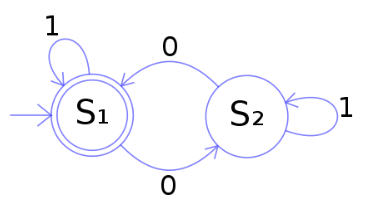
\includegraphics[scale=1.0]{figures/FSM.png}
  \end{center}
\end{examplebox}

Another common structure that is simple but powerful and used in
signal processing and control is {\em linear time-invariant (LTI)
    systems}\index{linear time-invariant systems}.  In this case, all
the quantities are real-valued vectors: $\mathcal S = \R^m$, $\mathcal
  X = \R^l$ and $\mathcal Y = \R^n$. The functions $f_s$ and $f_o$ are
linear functions of their inputs.
The transition function is described by the state matrix $A$ and the input matrix $B$;
the output function is defined by the output matrix $C$, each with compatible dimensions.
In discrete time, they can be
defined by a linear difference equation, like
\begin{align}
  s_t & = f_s(s_{t-1}, x_t) = A s_{t-1} + B x_t, \\
  y_t & = f_o(s_t) = C s_t, \;\;
\end{align}
and can be implemented using state to store relevant previous
input and output information.
We will study {\it{recurrent neural networks}} which are a lot like a
non-linear version of an LTI system.


%%%%%%%%%%%%%%%%%%%%%%%%%%%%%%%%%%%%%%%%%%%%%%%%%%%%%%%%%%%%%%%%%%%%%%%%%%%%%
\section{Recurrent neural networks}
\label{sec-rnn_model}

In Chapter~\ref{chap-neural_networks}, we studied neural networks and
how the weights of a network can be obtained by training on data, so
that the neural network will model a function that approximates the
relationship between the $(x, y)$ pairs in a supervised-learning
training set.  In Section~\ref{sec-state_machines} above, we
introduced state machines to describe sequential temporal
behavior. Here in Section~\ref{sec-rnn_model}, we explore recurrent
neural networks by defining the architecture and weight matrices in a
neural network to enable modeling of such state machines.  Then, in
Section~\ref{sec-seq2seq_rnn}, we present a loss function that may be
employed for training {\em sequence to sequence} {\sc rnn}s, and then
consider application to language translation and recognition in
Section~\ref{sec-language}.  In Section~\ref{sec-bptt}, we'll see how
to use gradient-descent methods to train the weights of an {\sc rnn}
so that it performs a {\em transduction} that matches as closely as
possible a training set of input-output {\em sequences}.

\bigskip

\begin{comment}
Recall that the basic operation of the state machine is to
start with some state $s_0$, then iteratively compute for $t \geq 1$:
\begin{align}
  s_t & = f_s(s_{t - 1}, x_t) \\
  y_t & =  f_o(s_t)
\end{align}
as illustrated in the diagram below (remembering that there needs to
be a delay on the feedback  loop):
\begin{center}
  \tikzstyle{block} = [draw, fill=blue!20, rectangle, minimum height=3em, minimum width=3em]
  \tikzstyle{sum} = [draw, fill=blue!20, circle, node distance=1cm]
  \tikzstyle{input} = [coordinate]
  \tikzstyle{output} = [coordinate]
  \tikzstyle{pinstyle} = [pin edge={to-,thin,black}]

  % The block diagram code is probably more verbose than necessary
  \begin{tikzpicture}[auto, node distance=2cm,>=latex']
    % We start by placing the blocks
    \node [input, name=input] {};
    \node [block, right of=input, node distance=2cm] (f_s) {f_s};
    \node [block, right of=f,
      node distance=4cm] (f_o) {f_o};
    % We draw an edge between the controller and system block to 
    % calculate the coordinate u. We need it to place the measurement block. 
    \draw [->] (f) -- node[name=u] {\hspace*{1cm} $s_t$} (f_o);
    \node [output, right of=f_o, node distance=2cm] (output) {};
    \node [coordinate, name=measurements, below of=f, node distance=2cm] (measurements) {Measurements};

    % Once the nodes are placed, connecting them is easy. 
    \draw [draw,->] (input) -- node {$x_t$} (f_s);
    \draw [->] (f_o) -- node [name=y_t] {$y_t$}(output);
    \draw [->] (u) |- (measurements);
    \draw [->] (measurements) -| node[pos=0.98] {$-$}
    node [near end] {$s_{t - 1}$} (f_s);
  \end{tikzpicture}
\end{center}
So, given a sequence of inputs $x_1, x_2, \dots$ the machine generates a
sequence of outputs
\begin{equation}
  \underbrace{f_o(f_s(s_0, x_1))}_{y_1}, \underbrace{f_o(f_s(f_s(s_0, x_1), x_2))}_{y_2}, \dots \;\;.
\end{equation}
\end{comment}

A {\it recurrent neural network}\index{recurrent neural network} is a state machine with neural
networks constituting functions $f_s$ and $f_o$:
\begin{align}
  s_t & = f_s\left(W^{sx}x_t + W^{ss}s_{t - 1} + W^{ss}_0\right) \\
  y_t & = f_o\left(W^o s_t + W_0^o\right) \;\;.
\end{align}
% \note{We are very sorry!   This course material has evolved from 
%   different sources, which used $W^Tx$ in the forward pass for regular
%   feedforward NNs and $Wx$ for the forward pass in {\sc rnn}s.  This
%   inconsistency  doesn't make any technical difference, but is a
%   potential source of confusion.
% }
The inputs, states, and outputs are all vector-valued:
\begin{align}
  x_t & : \ell \times 1    \\
  s_t & : m \times 1       \\
  y_t & : v \times 1 \;\;.
\end{align}
The weights in the network,  then,  are
\begin{align}
  W^{sx}   & :  m \times \ell \\
  W^{ss}   & : m \times m     \\
  W^{ss}_0 & : m \times 1     \\
  W^{o}    & : v \times m     \\
  W^{o}_0  & : v \times 1
\end{align}
with activation functions $f_s$  and $f_o$.

\question{Check dimensions here to be sure it all works out.  Remember
  that we apply $f_s$ and $f_o$ elementwise, unless $f_o$ is a
  softmax activation.}

%%%%%%%%%%%%%%%%%%%%%%%%%%%%%%%%%%%%%%%%%%%%%%%%%%%%%%%%%%%%%%%%%%%%%%%%%%%%%
\section{Sequence-to-sequence RNN}

\label{sec-seq2seq_rnn}

Now, how can we set up an {\sc rnn} to model and be trained to produce
a transduction\index{transduction} of one sequence to another?  This problem is sometimes
called {\em sequence-to-sequence} mapping\index{sequence-to-sequence mapping}.  You can think of it as a
kind of regression problem: given an input sequence, learn to generate
the corresponding output sequence. \note{One way to think of training
  a sequence {\bf classifier} is to reduce it to a transduction
  problem, where $y_t = 1$ if the sequence $x_1, \ldots, x_t$ is a
    {\em positive} example of the class of sequences and $-1$
  otherwise.}

A training  set has the form
$\left[\left(x^{(1)}, y^{(1)}\right), \dots, \left(x^{(q)},
    y^{(q)}\right)\right]$, where
\begin{itemize}
  \item
        $x^{(i)}$ and $y^{(i)}$ are length $n^{(i)}$ sequences;
  \item
        sequences in the {\it{same pair}} are the same length; and
        sequences in different pairs may have different lengths.
\end{itemize}

Next, we need a loss function.  We start by defining a loss function
on sequences.  There are many possible choices, but usually it makes
sense just to sum up a per-element loss function on each of the output
values, where $g$ is the predicted sequence and $y$ is the actual one:
\begin{equation}
  \mathcal{L}_{\text{seq}}\left(g^{(i)}, y^{(i)}\right) = \sum_{t =
    1}^{n^{(i)}}\mathcal{L}_\text{elt}\left(g_t^{(i)},
  y_t^{(i)}\right) \;\;.
\end{equation}
The per-element loss function $\mathcal{L}_\text{elt}$\note{So it could be  {\sc nll},
  squared loss, etc.}\ will depend on
the type of $y_t$
and what information it is encoding, in the same way as for a
supervised network.

Then, letting $W =\left(W^{sx}, W^{ss}, W^o, W^{ss}_0,
  W_0^o\right)$, our overall goal is to minimize the objective
\begin{equation}
  J(W) = \frac{1}{q} \sum_{i = 1}^q\mathcal{L}_{\text{seq}}\left(
  \text{RNN}(x^{(i)};W), y^{(i)}\right) \;\;,
\end{equation}
where $\text{RNN}(x; W)$ is the output sequence generated, given
input sequence $x$.

It is typical to choose $f_s$ to be {\it tanh} \note{Remember that it
  looks like a sigmoid but ranges from -1 to +1.} but any non-linear
activation function is usable.  We choose  $f_o$ to align with the
types of our outputs and the loss function,  just as we would do in
regular supervised learning.


\section{RNN as a language model}
\label{sec-language}

A {\em language model}\index{language model} is a sequence to sequence {\sc rnn} which is
trained on a token\note{A ``token'' is generally a
  character, common word fragment, or a word.} sequence of the form, $c = (c_1, c_2,
  \ldots, c_k)$, and is used to predict the next token $c_t, t \leq k$,
given a sequence of the previous $(t-1)$ tokens:
\begin{equation}
  c_t = \text{RNN}\left((c_1, c_2, \dots, c_{t - 1}) ; W \right)\;\;
\end{equation}

We can convert this to a sequence-to-sequence training problem by
constructing a data set of $q$ different $(x, y)$ sequence pairs, where we make up
new special tokens, $\text{start}$ and $\text{end}$, to signal the
beginning and end of the sequence:
\begin{align}
  x & = (\langle\text{start}\rangle, c_1, c_2, \ldots, c_k) \\
  y & = (c_1, c_2, \dots, \langle\text{end}\rangle)
\end{align}



%%%%%%%%%%%%%%%%%%%%%%%%%%%%%%%%%%%%%%%%%%%%%%%%%%%%%%%%%%%%%%%%%%%%%%%%%%%%%

% \begin{noticebox}
%   The following material on back-propagation through time
%   (Section~\ref{sec-bptt}) and vanishing gradients and gating
%   mechanisms (Section~\ref{sec-rnn_lstm}) is for your own elucidation.
%   It is not being covered in the Fall 2021 semester of 6.036, and will
%   not be included in the final exam.
% \end{noticebox}

\section{Back-propagation through time}
\label{sec-bptt}

Now the fun begins!  We can now try to find a $W$ to minimize $J$
using gradient descent.  We will work through the simplest method,
{\em back-propagation through time}\index{backpropagation through
  time} ({\sc bptt}), in detail.  This is generally not the best
method to use, but it's relatively easy to understand.  In
Section~\ref{lstm} we will sketch alternative methods that are in much
more common use.

\bigskip
\begin{noticebox}
  What we want you to take away from this section is that, by
  ``unrolling'' a recurrent network out to model a particular
  sequence, we can treat the whole thing as a feed-forward network
  with a lot of parameter sharing.  Thus, we can tune the parameters
  using stochastic gradient descent, and learn to model sequential
  mappings.  The concepts here are very important.  While the details
  are important to get right if you need to implement something, we
  present the mathematical details below primarily to convey or
  explain the larger concepts.
\end{noticebox}


\begin{examplebox} {\bf Calculus reminder: total derivative} Most of
  us are not very careful about the difference between the {\em
      partial derivative} and the {\em total derivative}\index{total derivative}.  We are going
  to use a nice example from the Wikipedia article on partial
  derivatives to illustrate the difference.

  The volume of a circular cone depends on its height and radius:
  \begin{equation}
    V(r, h) = \frac{\pi r^2 h}{3}\;\;.
  \end{equation}
  The partial derivatives of volume with respect to height and radius
  are
  \begin{equation}
    \frac{\partial V}{\partial r} = \frac{2\pi r
      h}{3}\;\;\;\text{and}\;\;\;
    \frac{\partial V}{\partial h} = \frac{\pi r^2}{3}\;\;.
  \end{equation}
  They measure the change in $V$ assuming everything is held constant
  except the single variable we are changing.
  Now assume that we want to preserve the cone's proportions in the sense that the ratio of radius to height stays constant.
  Then we can't really change one without changing the other.
  In this case, we really have to think about the {\em total derivative}.
  If we're interested in the total derivative with respect to $r$, we sum the ``paths'' along which $r$ might influence $V$:
  \begin{align}
    \frac{dV}{dr} & = \frac{\partial V}{\partial r} + \frac{\partial
    V}{\partial h} \frac{dh}{dr}                                            \\
                  & = \frac{2 \pi r h}{3} + \frac{\pi r^2}{3} \frac{dh}{dr}
  \end{align}
  Or if we're interested in the total derivative with respect to $h$, we consider how $h$ might influence $V$, either directly or via $r$:
  \begin{align}
    \frac{dV}{dh} & = \frac{\partial V}{\partial h} + \frac{\partial
    V}{\partial r} \frac{dr}{dh}                                            \\
                  & = \frac{\pi r^2}{3} + \frac{2 \pi r h}{3} \frac{dr}{dh}
  \end{align}

  Just to be completely concrete, let's think of a right circular cone
  with a fixed angle $\alpha = \tan r / h$, so that if we change $r$ or
  $h$ then $\alpha$ remains constant.  So we have $r = h \tan^{-1}
    \alpha$;  let constant $c = \tan^{-1} \alpha$, so now $r = c h$.
  Thus, we finally have
  \begin{align}
    \frac{dV}{dr} & = \frac{2 \pi r h}{3} + \frac{\pi r^2}{3} \frac{1}{c} \\
    \frac{dV}{dh} & = \frac{\pi r^2}{3} + \frac{2 \pi r h}{3} c \; .
  \end{align}

\end{examplebox}

\noindent The {\sc bptt} process goes like this:
\begin{enumerate}[(1)]
  \item
        Sample a training pair of  sequences $(x, y)$; let their length be $n$.
  \item
        ``Unroll" the RNN to be length $n$ (picture for $n = 3$ below), and
        initialize $s_0$:

        \centerline{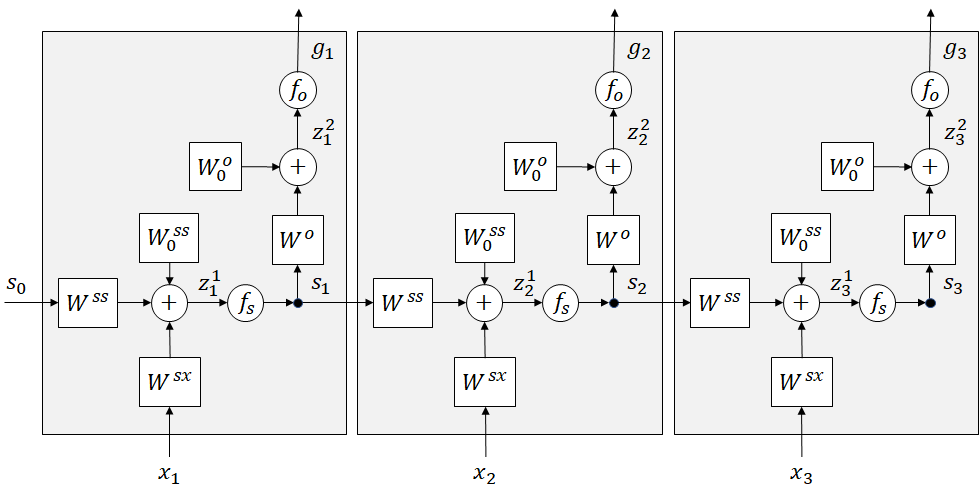
\includegraphics[width=\textwidth]{figures/rnn_unrolled_with_offsets.png}}

        Now,  we can see our problem as one of performing what is almost an
        ordinary back-propagation training procedure in a feed-forward neural
        network, but with the difference that the weight matrices are shared
        among the layers.  In many ways, this is similar to what ends up
        happening in a convolutional network, except in the conv-net, the
        weights are re-used spatially, and here, they are re-used temporally.
  \item
        Do the {\it forward pass}, to compute the predicted output sequence $g$:
        \begin{align}
          z_t^1 & = W^{sx}x_t + W^{ss}s_{t - 1} + W^{ss}_0 \\
          s_t   & = f_s(z_t^1)                             \\
          z_t^2 & = W^os_t + W_0^o                         \\
          g_t   & = f_o(z_t^2)
        \end{align}
  \item
        Do {\em backward pass} to compute the gradients. For both $W^{ss}$ and
        $W^{sx}$ we need to find
        \begin{align}
          \frac{d \mathcal{L}_\text{seq}(g,y)}{d W} & = \sum_{u = 1}^n\frac{d \mathcal{L}_\text{elt}(g_u, y_u)}{d W} ~~~~~~~~~~~~~~~~~~ \nonumber
        \end{align}
        Letting $\mathcal{L}_u = \mathcal{L}_\text{elt}(g_u, y_u)$ and using the {\em  total derivative}, which is a sum over all
        the ways in which $W$ affects $\mathcal{L}_u$, we have
        \begin{align}
          ~~~~ & = \sum_{u = 1}^n\sum_{t = 1}^n  \frac{\partial s_t}{\partial W} \frac{\partial \mathcal{L}_u}{\partial s_t}  \nonumber
        \end{align}
        Re-organizing, we have
        \begin{align}
          ~~~~ & = \sum_{t = 1}^n\frac{\partial s_t}{\partial W} \sum_{u =
            1}^n\frac{\partial \mathcal{L}_u}{\partial s_t} \nonumber
        \end{align}
        Because $s_t\ \text{only affects}\ \mathcal{L}_t, \mathcal{L}_{t + 1}, \dots, \mathcal{L}_n$,
        \begin{align}
          ~~~~~~~~~~~~~~~~~~~~ & = \sum_{t = 1}^n\frac{\partial s_t}{\partial W} \sum_{u = t}^n\frac{\partial \mathcal{L}_u}{\partial s_t} \nonumber \\
                               & = \sum_{t = 1}^n\frac{\partial s_t}{\partial W}
          \left(\frac{\partial \mathcal{L}_t}{\partial s_t} + \underbrace{\sum_{u = t +
              1}^n\frac{\partial \mathcal{L}_u}{\partial s_t}}_{\delta^{s_t}}\right) \; .\label{sumeq}
        \end{align}
        where $\delta^{s_t}$ is the dependence of the future loss (incurred after step $t$) on the
        state $S_t$.\note{That is, $\delta^{s_t}$ is how much we can
          blame state $s_t$ for all the future element losses.}

        We can compute this backwards, with $t$ going from $n$ down to $1$.
        The trickiest part is figuring out how early states contribute to later
        losses. We define the {\it{future loss}} after step $t$ to be
        \begin{equation}
          F_t = \sum_{u = t + 1}^{n}\mathcal{L}_\text{elt}(g_u, y_u) \;\;,
        \end{equation}
        so
        \begin{equation}
          \delta^{s_t} = \frac{\partial F_t}{\partial s_t}\;\;.
        \end{equation}
        At the last stage, $F_n = 0$ so $\delta^{s_n} = 0$.

        Now, working backwards,
        \begin{align}
          \delta^{s_{t -1}} & = \frac{\partial}{\partial s_{t - 1}}\sum_{u = t}^n\mathcal{L}_\text{elt}(g_u, y_u)                                                                                       \\
                            & = \frac{\partial s_t}{\partial s_{t - 1}} \frac{\partial}{\partial s_t}\sum_{u = t}^n\mathcal{L}_\text{elt}(g_u, y_u)                                                     \\
                            & = \frac{\partial s_t}{\partial s_{t - 1}} \frac{\partial}{\partial s_t}\left[\mathcal{L}_\text{elt}(g_t, y_t) + \sum_{u = t + 1}^n\mathcal{L}_\text{elt}(g_u, y_u)\right] \\
                            & = \frac{\partial s_t}{\partial s_{t - 1}} \left[\frac{\partial \mathcal{L}_\text{elt}(g_t, y_t)}{\partial s_t} + \delta^{s_t}\right]
        \end{align}
        Now, we can use the chain rule again to find the dependence of the
        element loss at time $t$ on the state  at that same time,
        \begin{equation}
          \underbrace{\frac{\partial \mathcal{L}_\text{elt}(g_t,
              y_t)}{\partial s_t}}_{(m \times 1)} = \underbrace{\frac{\partial
              z_t^2}{\partial s_t}}_{(m \times v)} ~
          \underbrace{\frac{\partial \mathcal{L}_\text{elt}(g_t, y_t)}{\partial
              z_t^2}}_{(v \times 1)}\;\;,
        \end{equation}
        and the dependence of the state at time $t$ on the state at the
        previous  time,
        %noting that we are performing an {\em elementwise}
        %multiplication between $W^T_{ss}$ and the vector of ${f^1}'$ values, $\partial
        %s_t /\partial z^1_t$:
        \iffalse
          \note{There  are two ways  to think about $\partial s_t  / \partial
              z_t$:  here, we take the view  that it is an $m \times 1$ vector and
            we multiply each column of $W^T$ by it.  Another, equally good,
            view, is that it is an $m \times m$ diagonal matrix, with the values
            along the diagonal, and then  this operation is a matrix multiply.
            Our software implementation will take the first view.
          }
        \fi
        \begin{equation}
          \underbrace{\frac{\partial s_t}{\partial s_{t - 1}}}_{(m \times m)}
          = \underbrace{\frac{\partial z_t^1}{\partial s_{t - 1}}}_{(m \times
            m)} \underbrace{\frac{\partial s_t}{\partial z_t^1}}_{(m
            \times m)} = {W^{ss}}^T \frac{\partial s_t}{\partial z_t^1}
        \end{equation} \\
        \begin{examplebox} Note that $\partial s_t /\partial z^1_t$
          is formally an $m \times m$ diagonal matrix, with the values
          along the diagonal being $f_{s}'(z_{t,i}^1)$, $1 \leq i \leq m$. But since this is a diagonal matrix, one could represent it as an $m \times 1$ vector $f_{s}'(z_t^1)$. In that case the product of the matrix ${W^{ss}}^T$ by the vector $f_{s}'(z_t^1)$, denoted ${W^{ss}}^T * f_{s}'(z_t^1)$, should be interpreted as follows: take the first column of the matrix ${W^{ss}}^T$ and multiply each of its elements by the first element of the vector $\partial s_t /\partial z^1_t$, then take the second column of the matrix ${W^{ss}}^T$ and multiply each of its elements by the second element of the vector $\partial s_t /\partial z^1_t$, and so on and so forth ...
        \end{examplebox}

        Putting this all together, we end up with
        \begin{equation}
          \delta^{s_{t - 1}} = \underbrace{{W^{ss}}^T \frac{\partial s_t}{\partial z_t^1}}_{\frac{\partial s_t}{\partial s_{t - 1}}} ~ \underbrace{\left({W^o}^T\frac{\partial{\mathcal{L}_t}}{\partial z_t^2} + \delta^{s_t}\right)}_{\frac{\partial F_{t - 1}}{\partial s_t}}
        \end{equation}

        We're almost there!  Now, we can describe the actual weight updates.
        Using Eq.~\ref{sumeq} and recalling the definition of
        $\delta^{s_t} = \partial F_t / \partial s_t$,
        as we iterate backwards, we can accumulate the terms in Eq.~\ref{sumeq}
        to get the gradient for the whole  loss.
        \iffalse
          \begin{align}
            \frac{ d \mathcal{L}_\text{seq}}{d W^{ss}} & +=
            \frac{\partial F_{t-1}}{\partial W^{ss}} =
            \frac{\partial z^1_t}{\partial W^{ss}} \frac{\partial s_t}{\partial z^1_t}
            \frac{\partial F_{t-1}}{\partial s_t}           \\
            \frac{ d \mathcal{L}_\text{seq}}{d W^{sx}} & +=
            \frac{\partial F_{t-1}}{\partial W^{sx}} =
            \frac{\partial z^1_t}{\partial W^{sx}} \frac{\partial s_t}{\partial z^1_t}
            \frac{\partial F_{t-1}}{\partial s_t}
          \end{align}
        \fi



        \begin{align}
          \frac{d \mathcal{L}_\text{seq}}{d W^{ss}} & = \sum_{t=1}^n
          \frac{d \mathcal{L}_\text{elt}(g_t, y_t)}{d W^{ss}} = \sum_{t=1}^n \frac{\partial z_t^1}{\partial W^{ss}} \frac{\partial s_t}{\partial z_t^1} \frac{\partial F_{t - 1}}{\partial s_t} \\
          \frac{d \mathcal{L}_\text{seq}}{d W^{sx}} & =  \sum_{t=1}^n
          \frac{d \mathcal{L}_\text{elt}(g_t, y_t)}{d W^{sx}} = \sum_{t=1}^n
          \frac{\partial z_t^1}{\partial W^{sx}} \frac{\partial s_t}{\partial z_t^1} \frac{\partial F_{t-1}}{\partial s_t}
        \end{align}
        We can handle $W^o$ separately;   it's easier because it does not
        affect future  losses  in the way that the other weight matrices do:
        \begin{equation}
          \frac{d\mathcal{L}_\text{seq}}{d W^o} = \sum_{t = 1}^n\frac{d \mathcal{L}_t}{d W^o} = \sum_{t = 1}^n\frac{\partial \mathcal{L}_t}{\partial
            z_t^2} \frac{\partial z_t^2}{\partial W^o}
        \end{equation}
        Assuming we have $\frac{\partial \mathcal{L}_t}{\partial z_t^2} = (g_t - y_t)$,
        (which ends up being true for squared loss, softmax-NLL, etc.), then
        \begin{equation}
          \underbrace{\frac{d \mathcal{L}_\text{seq}}{d W^o}}_{v \times m} = \sum_{t=1}^n \underbrace{(g_t - y_t)}_{v \times 1} ~ \underbrace{s_t^T}_{1 \times m} \; .
        \end{equation}

        Whew!
\end{enumerate}
\question{Derive the updates for the offsets $W^{ss}_0$ and $W^o_0$.}

%%%%%%%%%%%%%%%%%%%%%%%%%%%%%%%%%%%%%%%%%%%%%%%%%%%%%%%%%%%%%%%%%%%%%%%%%%%%%
\section{Vanishing gradients and gating mechanisms}
\label{lstm}
\label{sec-rnn_lstm}

Let's take a careful look at the backward propagation of the gradient
along the sequence:
\begin{equation}
  \delta^{s_{t -1}} = \frac{\partial s_t}{\partial s_{t - 1}} ~
  \left[\frac{\partial \mathcal{L}_\text{elt}(g_t, y_t)}{\partial s_t}
    + \delta^{s_t}\right]\;\;.
\end{equation}
Consider a case where only the output at the end of the sequence is
incorrect, but it depends critically, via the weights,  on the input
at time 1.   In this case, we will multiply the loss at step $n$ by
\begin{equation}
  \frac{\partial s_2}{\partial s_1} \frac{\partial s_3}{\partial
    s_2} \cdots \frac{\partial s_n}{\partial s_{n-1}}\;\;.
\end{equation}
In general, this quantity will either grow or shrink exponentially
with the length of the sequence, and make it very difficult to train.
\question{The last time we talked about exploding and vanishing
  gradients, it was to justify per-weight adaptive step sizes.  Why is
  that not a solution to the problem this time?}

An important insight that really made recurrent networks work well on
long sequences is the idea of {\em gating}\index{recurrent neural network!gating}.

\subsection{Simple gated recurrent networks}

A computer only ever updates some parts of its memory on each
computation cycle.  We can take this idea and use it to make our
networks more able to retain state values over time and to make the
gradients better-behaved.  We will add a new component to our network,
called a {\em gating network}\index{gating network}.  Let $g_t$ be a $m \times 1$ vector of
values and let $W^{gx}$ and $W^{gs}$ be $m \times l$ and $m \times m$
weight matrices, respectively.  We will compute $g_t$ as
\note{It can have an offset, too, but we are omitting it for simplicity.}
\begin{equation}
  g_t = \text{sigmoid}(W^{gx} x_t + W^{gs} s_{t-1})
\end{equation}
and then change the computation of $s_t$ to be
\begin{equation}
  s_t = (1 - g_t) *  s_{t-1} + g_t * f_s(W^{sx}x_t + W^{ss}
  s_{t-1} + W^{ss}_0)\;\;,
\end{equation}
where $*$ is component-wise multiplication.  We can see, here, that
the output of the gating network is deciding, for each dimension of
the state, how much it should be updated now.  This mechanism makes it
much easier for the network to learn to,  for example, ``store'' some
information in some dimension of the state, and then not change it
during future state updates, or change it only under certain
conditions on the input or other aspects of the state.
\question{Why is it important that the activation function for $g$ be
  a sigmoid?}

\subsection{Long short-term memory}

The idea of gating networks can be applied to make a state machine
that is even more like a computer memory, resulting in a type of
network called an {\sc  lstm}\index{long short-term memory} for ``long short-term memory.''
\note{Yet another awesome name for a neural network!}  We won't go
into the details here,  but the basic idea is that there is a memory
cell (really, our state vector) and three (!) gating networks.  The
  {\em input} gate selects (using a ``soft''  selection as in the gated
network above) which dimensions of the state will be updated  with new
values;  the {\em forget} gate decides which dimensions of the state
will have its old values  moved toward 0, and the {\em  output} gate
decides which dimensions of the state will be used to compute the
output value.  These networks have been used in applications like
language translation with really amazing results.  A diagram of the
architecture is shown below:
\begin{center}
  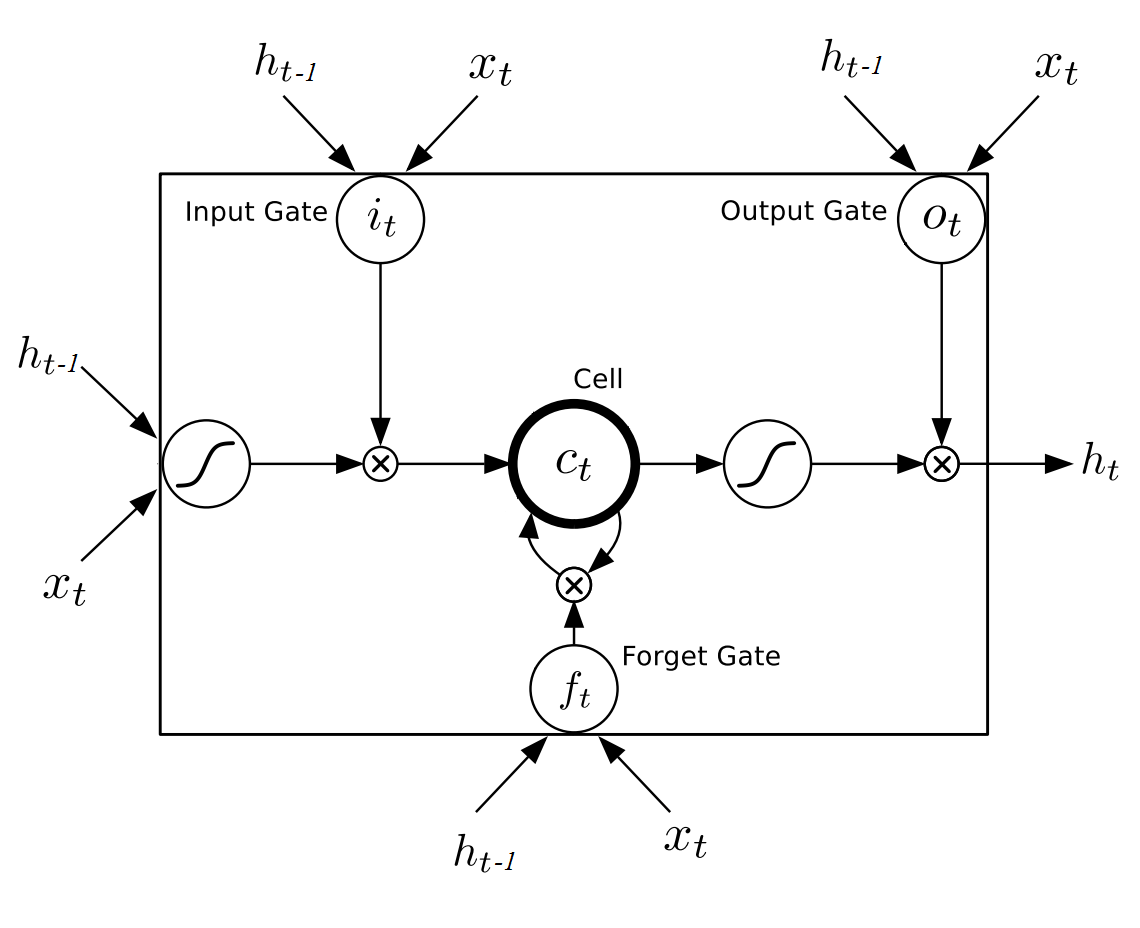
\includegraphics[scale = 0.7]{figures/lstm.png}
\end{center}


%%% Local Variables:
%%% mode: latex
%%% TeX-master: "top"
%%% End:


    \chapter{Supervised learning in a nutshell}
\label{sec-nutshell}

In which we try to describe the outlines of the ``lifecycle'' of
supervised learning, including hyperparameter tuning and evaluation of
the final product.

\section{General case}

We start with a very generic setting.

\subsection{Minimal problem specification}
Given:
\begin{itemize}
  \item Space of inputs $\mathcal{X}$
  \item Space of outputs $\mathcal{Y}$
  \item Space of possible {\em hypotheses} $\hclass$ such that each
        $h \in \hclass$ is a function
        $h: \mathcal{X} \rightarrow \mathcal{Y}$
  \item Loss function $\loss : \mathcal{Y} \times \mathcal{Y}
          \rightarrow \R$
\end{itemize}
a {\em supervised learning algorithm} $\alg$
takes as input a {\em data set} of the form
\[\data = \left\{\left(\ex{x}{1}, \ex{y}{1}\right), \dots,
  \left(\ex{x}{n}, \ex{y}{n}\right)\right\}\;\;,\]
where $\ex{x}{i} \in \mathcal{X}$ and $\ex{y}{i} \in \mathcal{Y}$
and returns an $h \in \hclass$.

\subsection{Evaluating a hypothesis}
Given a problem specification and a set of data $\data$, we
evaluate hypothesis $h$ according to average loss, or {\em error},
\begin{eqnarray*}
  \mathcal{E}(h, \loss, \data) = \frac{1}{|\data|}\sum_{i = 1}^{\data}
  \loss(h(\ex{x}{i}), \ex{y}{i})
\end{eqnarray*}

If the data used for evaluation {\em were not used during learning
    of the hypothesis} then this is a reasonable estimate of how well
the hypothesis will make additional predictions on new data from the
same source.

\subsection{Evaluating a supervised learning algorithm}

A {\em validation strategy} $\mathcal{V}$ takes an algorithm
$\alg$, a loss function $\loss$, and a data source
$\data$ and produces a real number which measures how well $\alg$
performs on data from that distribution.

\subsubsection{Using a validation set}
In the simplest case, we can divide $\data$ into two sets,
$\data^\text{train}$ and $\data^\text{val}$, train on the first, and
then evaluate the resulting hypothesis on the second.  In that case,
\[\mathcal{V}(\alg, \loss, \data) =
  \mathcal{E}(\alg(\data^\text{train}),
  \loss, \data^\text{val})\;\;.\]

\subsubsection{Using multiple training/evaluation runs}
We can't reliably evaluate an algorithm based on a single application of it to
a single training and test set, because there are many aspects of the
training and testing data, as well as, sometimes, randomness in
the algorithm itself, that cause {\em variance} in the performance of
the algorithm.  To get a good idea of how well an algorithm
performs, we need to, multiple times, train it and evaluate the
resulting hypothesis, and report the average over
$K$ executions of the algorithm of the error of the
hypothesis it produced each time.

We divide the data into $2K$ random non-overlapping subsets:
$\data_1^\text{train}, \data_1^\text{val}, \ldots,
  \data_K^\text{train}, \data_K^\text{val}.$    Then,
\[\mathcal{V}(\alg, \loss, \data) =
  \frac{1}{K}\sum_{k=1}^K \mathcal{E}(\alg(\data_k^\text{train}),
  \loss, \data_k^\text{val})\;\;.\]

\subsubsection{Cross validation}
In {\em cross validation}, we do a similar computation, but allow data
to be re-used in the $K$ different iterations of training and testing
the algorithm (but never share training and testing data for a single
iteration!).  See Section~\ref{cross-validation} for details.

\subsection{Comparing supervised learning algorithms}
Now, if we have two different algorithms $\alg_1$  and
$\alg_2$, we might be interested in knowing which one will
produce hypotheses that generalize the best, using data from a
particular source.   We could compute
$\mathcal{V}(\alg_1, \loss, \data)$ and
$\mathcal{V}(\mathcal{A_2}, \loss, \data)$, and prefer the
algorithm with lower validation error.  More generally, given
algorithms $\alg_1, \ldots, \alg_M$, we would prefer
\[\alg^* = \argmin{m} \mathcal{V}(\alg_M, \loss, \data)\;\;.\]

\subsection{Fielding a hypothesis}

Now what?  We have to deliver a hypothesis to our customer.
We now know how to find the algorithm, $\alg^*$, that works best for
our type of data.  We can apply it to all of our data to get the best
hypothesis we know how to create, which would be
\[h^* = \alg^*(\data)\;\;,\]
and deliver this resulting hypothesis as our best product.

\subsection{Learning algorithms as optimizers}
A majority of learning algorithms have the form of
optimizing some objective involving the training data and a loss
function.  \note{Interestingly, this loss function is {\em not always
      the same} as the loss function that is used for evaluation!  We
  will see this in logistic regression.}

So for example, (assuming a perfect optimizer which doesn't, of
course, exist) we might say our algorithm is to solve an optimization
problem:
\[\alg(\data) = \argmin{h \in H} \mathcal{J}(h; \data)\;\;.\]
Our objective often has the form
\[\mathcal{J}(h; \data) = \mathcal{E}(h,\loss, \data) +
  \mathcal{R}(h)\;\;,\]
where $\loss$ is a loss to be minimized during training and
$\mathcal{R}$ is a regularization term.

\subsection{Hyperparameters}
Often, rather than comparing an arbitrary collection of learning algorithms,
we think of our learning algorithm as having some parameters that
affect the way it maps data to a hypothesis.  These are not
parameters of the hypothesis itself, but rather parameters of the
  {\em algorithm}.  We call these {\em hyperparameters}.  A classic
example would be to use a hyperparameter $\lambda$ to govern the weight of a
regularization term on an objective to be optimized:
\[\mathcal{J}(h; \data) = \mathcal{E}(h,\loss, \data) +
  \lambda \mathcal{R}(h)\;\;.\]
Then we could think of our algorithm as $\alg(\data;
  \lambda)$.
Picking a good value of $\lambda$ is the same as comparing different
supervised learning algorithms, which is accomplished by validating
them and picking the best one!

\section{Concrete case: linear regression}
In linear regression the problem formulation is this:
\begin{itemize}
  \item $\mathcal{X} = \R^d$
  \item $\mathcal{Y} = \R$
  \item $\hclass = \{\theta^T x + \theta_0\}$ for values of
        parameters $\theta \in \R^d$ and $\theta_0 \in \R$.
  \item $\loss(g, y) = (g - y)^2$
\end{itemize}

Our learning algorithm has hyperparameter $\lambda$ and can be written
as:
\[\alg(\data; \lambda) = \Theta^*(\lambda, \data) = \argmin{\theta, \theta_0}
  \frac{1}{|\data|} \sum_{(x, y) \in \data} (\theta^Tx +
  \theta_0 - y)^2 + \lambda\|\theta\|^2 \;\;.\]
For a particular training data set and parameter $\lambda$, it finds
the best hypothesis on this data, specified with parameters $\Theta =
  (\theta, \theta_0)$, written  $\Theta^*(\lambda, \data)$.

Picking the best value of the hyperparameter is choosing among
learning algorithms. We could, most simply,
optimize using a single training / validation split, so $\data =
  \data^\text{train} \cup \data^\text{val}$, and
\begin{align*}
  \lambda^* & = \argmin{\lambda} \mathcal{V}(\alg_\lambda, \loss,
  \data^\text{val})                                                                             \\
            & = \argmin{\lambda} \mathcal{E}(\Theta^*(\lambda, \data^\text{train}), \text{mse},
  \data^\text{val})                                                                             \\
            & = \argmin{\lambda} \frac{1}{|\data_\text{val}|} \sum_{(x, y) \in
  \data_\text{val}} (\theta^*(\lambda, \data^\text{train})^T x +
  \theta^*_0(\lambda, \data^\text{train}) - y)^2
\end{align*}
It would be much better to select the best $\lambda$ using multiple
runs or cross-validation;  that would just be a different choices of
the validation procedure $\mathcal{V}$ in the top line.

Note that we don't use regularization here because we just want to measure how good the
output of the algorithm is at predicting values of {\em new} points,
and so that's what we measure.   We use the regularizer during
training when we don't want to focus only on optimizing predictions on
the training data.

Finally!  To make a predictor to ship out into the world, we would use
all the data we have, $\data$, to train, using the best
hyperparameters we know, and return
\begin{align*}
  \Theta^* & = \alg(\data; \lambda^*)     \\
           & = \Theta^*(\lambda^*, \data) \\
           & = \argmin{\theta, \theta_0}
  \frac{1}{|\data|} \sum_{(x, y) \in \data} (\theta^Tx +
  \theta_0 - y)^2 + \lambda^*\|\theta\|^2 \\
\end{align*}

Finally, a customer might evaluate this hypothesis on their data,
which we have never seen during training or validation, as
\begin{align*}
  \mathcal{E}^\text{test} & = \mathcal{E}(\Theta^*, \text{mse},
  \data^\text{test})                                                                                             \\
                          & = \frac{1}{|\data^\text{test}|} \sum_{(x, y) \in \data^\text{test}} ({\theta^*}^Tx +
  \theta_0^* - y)^2                                                                                              \\
\end{align*}

Here are the same ideas, written out in informal pseudocode.
\begin{verbatim}
# returns theta_best(D, lambda)
define train(D, lambda):
    return minimize(mse(theta, D) + lambda * norm(theta)**2, theta)

# returns lambda_best using very simple validation
define simple_tune(D_train, D_val, possible_lambda_vals):
    scores = [mse(train(D_train, lambda), D_val)
                  for lambda in possible_lambda_vals]
    return possible_lambda_vals[least_index[scores]]

# returns theta_best overall
define theta_best(D_train, D_val, possible_lambda_vals):
  return train(D_train + D_val, 
               simple_tune(D_train, D_val, possible_lambda_vals))

# customer evaluation of the theta delivered to them
define customer_val(theta):
    return mse(theta, D_test)

\end{verbatim}

\section{Concrete case: logistic regression}
In binary logistic regression the problem formulation is as follows.
We are writing the class labels as 1 and 0.
\begin{itemize}
  \item $\mathcal{X} = \R^d$
  \item $\mathcal{Y} = \{+1, 0\}$
  \item $\hclass = \{\sigma(\theta^T x + \theta_0)\}$ for values of
        parameters $\theta \in \R^d$ and $\theta_0 \in \R$.
  \item $\loss(g, y) = \loss_{01}(g, h)$
  \item Proxy loss $\loss_\text{nll}(g, y) = -\left(y \log (g) + (1 - y)\log (1 -g)\right)$
\end{itemize}

Our learning algorithm has hyperparameter $\lambda$ and can be written
as:
\[\alg(\data; \lambda) = \Theta^*(\lambda, \data) = \argmin{\theta, \theta_0}
  \frac{1}{|\data|} \sum_{(x, y) \in \data} \loss_\text{nll}(\sigma(\theta^Tx +
  \theta_0), y) + \lambda\|\theta\|^2 \;\;.\]
For a particular training data set and parameter $\lambda$, it finds
the best hypothesis on this data, specified with parameters $\Theta =
  (\theta, \theta_0)$, written  $\Theta^*(\lambda, \data)$ according to
the proxy loss $\loss_\text{nll}$.

Picking the best value of the hyperparameter is choosing among
learning algorithms based on their actual predictions. We could, most simply,
optimize using a single training / validation split, so $\data =
  \data^\text{train} \cup \data^\text{val}$, and {\em we use the real
    01 loss}:
\begin{align*}
  \lambda^* & = \argmin{\lambda} \mathcal{V}(\alg_\lambda, \loss_{01},
  \data^\text{val})                                                                             \\
            & = \argmin{\lambda} \mathcal{E}(\Theta^*(\lambda, \data^\text{train}), \loss_{01},
  \data^\text{val})                                                                             \\
            & = \argmin{\lambda} \frac{1}{|\data_\text{val}|} \sum_{(x, y) \in
    \data_\text{val}} \loss_{01}(\sigma(\theta^*(\lambda, \data^\text{train})^T x +
  \theta^*_0(\lambda, \data^\text{train})), y)
\end{align*}
It would be much better to select the best $\lambda$ using multiple
runs or cross-validation;  that would just be a different choices of
the validation procedure $\mathcal{V}$ in the top line.

Finally!  To make a predictor to ship out into the world, we would use
all the data we have, $\data$, to train, using the best
hyperparameters we know, and return
\begin{align*}
  \Theta^* & = \alg(\data; \lambda^*)
\end{align*}
\question{What loss function is being optimized inside this algorithm?}

Finally, a customer might evaluate this hypothesis on their data,
which we have never seen during training or validation, as
\begin{align*}
  \mathcal{E}^\text{test} & = \mathcal{E}(\Theta^*, \loss_{01},
  \data^\text{test})
\end{align*}
The customer just wants to buy the right stocks!  So we use the real
$\loss_{01}$ here for validation.


%%% Local Variables:
%%% mode: latex
%%% TeX-master: "top"
%%% End:


    \printindex
    \clearpage
    \glsaddall
    \printglossaries
    \clearpage
\end{appendices}

%\chapter{The Perceptron}
\label{chap-perceptron}
First of all, the coolest algorithm name! \note{Well, maybe
  ``neocognitron,'' also the name of a real ML algorithm, is cooler.}
It is based on the 1943 model of neurons made by McCulloch and Pitts
and by Hebb.  It was developed by Rosenblatt in 1962.  At the time, it
was not interpreted as attempting to optimize any particular criteria;
it was presented directly as an algorithm.  There has, since, been a
huge amount of study and analysis of its convergence properties and
other aspects of its behavior.

\section{Algorithm}

Recall that we have a training dataset $\dataTrain$ with $x \in \R^d$,
and $y\in \{-1, +1\}$.  The Perceptron algorithm trains a binary
classifier $h(x; \theta, \theta_0)$ using the following algorithm to
find $\theta$ and $\theta_0$ using (at most) $\tau$ \anchorednote{iterative
  steps:}{We use Greek letter $\tau$ here instead of $T$ so we don't
  confuse it with transpose!}

\begin{codebox}
  \Procname{$\proc{Perceptron}(\tau, \dataTrain)$}
  \li $\theta \gets
    \begin{bmatrix}
      0 & 0 & \cdots & 0
    \end{bmatrix}^T$
  \li $\theta_0 \gets 0$
  \li \For $t \gets 1$ \To $\tau$
  \li   \Do
  changed = False
  \li        \For $i \gets 1$ \To $n$
  \li       \Do
  \If $\ex{y}{i}\left(\theta^T\ex{x}{i} + \theta_0\right) \le 0$
  \li           \Then
  $\theta \gets \theta + \ex{y}{i}\ex{x}{i}$
  \li             $\theta_0 \gets \theta_0 + \ex{y}{i}$
  \li             changed = True
  \End
  \End
  \li      \If {\sc not} changed
  \li          \Then
  break
  \End
  \End
  \li \Return $\theta, \theta_0$
\end{codebox}

\note{Let's check dimensions.  Remember that $\theta$ is $d \times 1$,
  $\ex{x}{i}$ is $d \times 1$, and $\ex{y}{i}$ is a scalar.  Does
  everything match?}

Intuitively, on each step, if the current hypothesis
$\theta, \theta_0$ classifies example $\ex{x}{i}$ correctly, then no
change is made.  If it classifies $\ex{x}{i}$ incorrectly, then it
moves $\theta, \theta_0$ so that it is ``closer'' to classifying
$x^{(i)}, y^{(i)}$ correctly.

Note that if the algorithm ever steps once through every value of $i$
without making an update, it will never make any further updates (this
is true even if the ``break'' statement were removed; verify that you
believe this!) and so it should just terminate at that point.
\question {\em What is true about $\trainerr$ if that happens?}

\begin{examplebox}{\bf Example:}
  Let $h$ be the linear classifier defined by $\ex{\theta}{0} =
    \protect\twodcol{1}{-1}, \ex{\theta_0}{0} = 1$.
  \noindent
  The diagram below shows several points classified by $h$.  However, in
  this case, $h$ (represented by the bold line and normal vector $\ex{\theta}{0}$) misclassifies the point
  $\ex{x}{1} = \twodcol{1}{3}$ which has label $\ex{y}{1} = 1$.  Indeed,
  $$ \ex{y}{1}\left(\theta^T \ex{x}{1} + \theta_0\right) =  \twodrow{1}{-1}
    \twodcol{1}{3} + 1 = -1 < 0 $$
  By running an iteration of the Perceptron algorithm, we update
  $$ \ex{\theta}{1} = \ex{\theta}{0} + \ex{y}{1}\ex{x}{1} = \twodcol{2}{2} $$
  $$ \ex{\theta_0}{1} = \ex{\theta_0}{0} + \ex{y}{1} = 2 $$
  The new classifier (represented by the dashed line and normal vector $\ex{\theta}{1}$) now correctly
  classifies that point, but now makes a mistake on the negatively
  labeled point.

  \begin{center}
    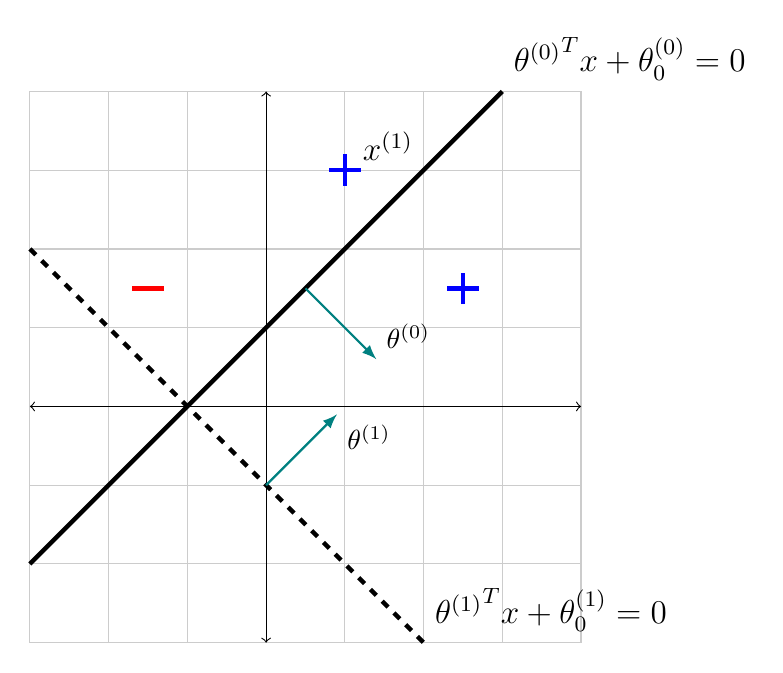
\begin{tikzpicture}
      \draw [thin, gray!40] (-3,-3) grid (4,4);
      \draw [<->] (-3,0) -- (4,0);
      \draw [<->] (0,-3) -- (0,4);

      \draw [ultra thick] (-3, -2) -- (3, 4)
      node [above right] {\large${\ex{\theta}{0}}^Tx + \ex{\theta_0}{0} = 0$};

      \draw [thick,teal,-latex] (0.5, 1.5) -- (1.4, 0.6)
      node [black,above right] {$\ex{\theta}{0}$};

      %  \draw [ultra thick, dashed] (-2, 4) -- (4, -2)
      \draw [ultra thick, dashed] (-3, 2) -- (2, -3)
      node [black,above right] {\large${\ex{\theta}{1}}^Tx + \ex{\theta_0}{1} = 0$};

      %  \draw [thick,teal,-latex] (1, 1) -- (1.9, 1.9)
      %  \draw [thick,teal,-latex] (-1, -1) -- (-0.1, -0.1)
      \draw [thick,teal,-latex] (0.0, -1.0) -- (0.9, -0.1)
      node [black,below right] {$\ex{\theta}{1}$};

      \node [above right,xshift=.3em] at (1,3) {\large$\ex{x}{1}$};
      \foreach \Point in {(1, 3), (2.5, 1.5)}{
          \pic at \Point {plus};
        }

      \foreach \Point in {(-1.5, 1.5)}{
          \pic at \Point {minus};
        }
    \end{tikzpicture}
  \end{center}
\end{examplebox}

A really important fact about the perceptron algorithm is that, if
there is a linear classifier with 0 training error, then
for large enough $\tau$
this algorithm will (eventually) find it!  We'll look at a proof of this in
detail, next.

\section{Offset}
\label{sec-offset}
Sometimes, it can be easier to implement or analyze classifiers of the
form
\begin{eqnarray*}
  h(x; \theta) =
  \begin{cases}
    +1 & \text{if } \theta^Tx > 0 \\
    -1 & \text{otherwise.}
  \end{cases}
\end{eqnarray*}
Without an explicit offset term ($\theta_0$), this separator must pass
through the origin, which may appear to be limiting. However, we can
convert any problem involving a linear separator \emph{with} offset
into one with \emph{no} offset (but of higher dimension)!

Consider the $d$-dimensional linear separator defined by
$\theta = \begin{bmatrix} \theta_1 & \theta_2 & \cdots
                         & \theta_d\end{bmatrix}$ and offset $\theta_0$.
\begin{itemize}
  \item for each data point
        $(x, y) \in \dataTrain$, append a coordinate with value +1 to $x$, yielding
        $$x_{\rm new} = \begin{bmatrix} x_1  & \cdots & x_d & +1 \end{bmatrix}^T$$
  \item define $$\theta_{\rm new} = \begin{bmatrix} \theta_1 & \cdots   &
                \theta_d & \theta_0\end{bmatrix}^T$$
\end{itemize}
Then,
\begin{align*}
  \theta_{\rm new}^T \cdot x_{\rm new} & = \theta_1x_1 + \cdots + \theta_dx_d
  + \theta_0 \cdot 1                                                          \\
                                       & = \theta^Tx + \theta_0
\end{align*}
Thus, $\theta_{\rm new}$ is an equivalent ($(d+1)$-dimensional) separator to
our original, but with no offset.

Consider the data set:
\begin{align*}
  X & = [[1], [2], [3], [4]]     \\
  Y & = [[+1], [+1], [-1], [-1]] \\
\end{align*}
It is linearly separable in $d = 1$ with $\theta = [-1]$ and $\theta_0
  = 2.5$.  But it is not linearly separable through the origin!   Now,
let
\[X_{\rm new} = \begin{bmatrix}
    \begin{bmatrix} 1 \\ 1 \end{bmatrix}
    \begin{bmatrix} 2 \\ 1 \end{bmatrix}
    \begin{bmatrix} 3 \\ 1 \end{bmatrix}
    \begin{bmatrix} 4 \\ 1 \end{bmatrix}
  \end{bmatrix}\]
This new dataset is separable through the origin, with $\theta_{\rm
    new} = [-1, 2.5]^T$.


% \lpknote{TAs:  Can you add the figure / example from the handwritten
%   notes?  (Just the example with 4 points going from 1 to 2
%   dimensions.)}

We can make a simplified version of the perceptron algorithm if we
restrict ourselves to separators through the origin: \note{We list it
  here because this is the version of the algorithm we'll study in
  more detail.}
\begin{codebox}
  \Procname{$\proc{Perceptron-Through-Origin}(\tau, \dataTrain)$}
  \li $\theta \gets
    \begin{bmatrix}
      0 & 0 & \cdots & 0
    \end{bmatrix}^T$
  \li \For $t \gets 1$ \To $\tau$
  \li   \Do
  changed = False
  \li      \For $i \gets 1$ \To $n$
  \li       \Do
  \If $\ex{y}{i}\left(\theta^T\ex{x}{i}\right) \le 0$
  \li           \Then
  $\theta \gets \theta + \ex{y}{i}\ex{x}{i}$
  \li             changed = True
  \End
  \End
  \li      \If {\sc not} changed
  \li          \Then
  break
  \End
  \li \Return $\theta$
\end{codebox}


\section{Theory of the perceptron}
Now, we'll say something formal about how well the perceptron
algorithm really works.  We start by characterizing the set of
problems that can be solved perfectly by the perceptron algorithm, and
then prove that, in fact, it can solve these problems.  In addition,
we provide a notion of what makes a problem difficult for perceptron
and link that notion of difficulty to the number of updates the
algorithm will make.

\subsection{Linear separability}
A training set $\dataTrain$ is {\em{linearly separable}} if there exist
$\theta, \theta_0$ such that, for all $i = 1, 2, \dots, n$:
$$ \ex{y}{i}\left(\theta^T\ex{x}{i} + \theta_0\right) > 0 \;\;.$$
Another way to say that $\dataTrain$ is linearly separable
is that there exists an $h$ such that all predictions on the training set
are correct,
$$ h(\ex{x}{i}; \theta, \theta_0) = \left(\theta^T\ex{x}{i} + \theta_0\right) =
  \ex{y}{i} \;\;,$$
in which case we call $h$ a {\em linear separator}.

And, another way to say that $\dataTrain$ is linearly separable
is that there exists an $h$ of the form above such that
the training error is zero,
$$\trainerr(h) = 0 \;\;.$$

\subsection{Convergence theorem}
The basic result about the perceptron is that, if the training data
$\dataTrain$ is linearly separable, then the perceptron algorithm is
guaranteed to find a linear separator, for large
enough $\tau.$ \note{If the training data is
    {\em not} linearly separable, the algorithm will not be able to tell
  you for sure, in finite time, that it is not linearly separable.
  There are other algorithms that can test for linear separability
  with run-times $O(n^{d/2})$ or $O(d^{2n})$ or $O(n^{d-1}\log{n})$.}

We will more specifically characterize the linear separability of the
dataset by the \emph{margin} of the separator.   We'll start by
defining the margin of a point with respect to a hyperplane.

First, recall that the signed distance from the
hyperplane $\theta, \theta_0$ to a point $x$ is
\[ \frac{\theta^Tx + \theta_0}{\norm{\theta}}\;\;. \]
Then, we'll define the {\em margin} of a {\em labeled point} $(x, y)$
with respect to hyperplane $\theta, \theta_0$ to be
\[ y \cdot \frac{\theta^Tx + \theta_0}{\norm{\theta}}\;\;. \]
This quantity will be positive if and only if the point $x$ is
classified as $y$ by the linear classifier represented by this
hyperplane.
\question{What sign does the margin have if the point is incorrectly
  classified?  Be sure you can explain why.}

Now, the {\em margin} of a {\em dataset} $\dataTrain$ with respect to the hyperplane
$\theta, \theta_0$ is the {\em minimum} margin of any point with respect
to $\theta, \theta_0$:
\[\min_i \left(\ex{y}{i} \cdot \frac{\theta^T \ex{x}{i} + \theta_0}{\norm{\theta}}\right)\;\;.\]
The margin is positive if and only if all of the points in the data-set
are classified correctly.  In that case (only!) it represents the
distance from the hyperplane to the closest point.

\begin{examplebox}{\bf Example:}
  Let $h$ be the linear classifier defined by $\theta = \protect\twodcol{1}{-1}, \theta_0 = 1$.

  \bigskip
  \noindent
  The diagram below shows several points classified by $h$, one of which is misclassified.  We compute the margin for each point:

  \begin{center}
    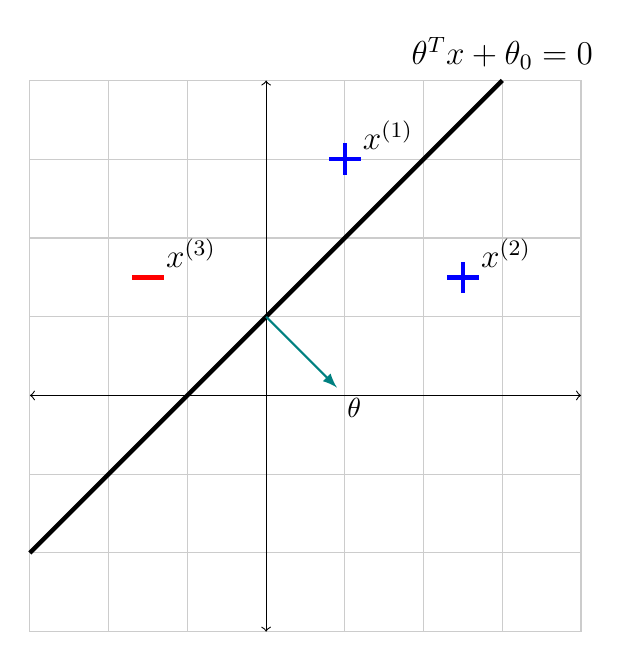
\begin{tikzpicture}
      \draw [thin, gray!40] (-3,-3) grid (4,4);
      \draw [<->] (-3,0) -- (4,0);
      \draw [<->] (0,-3) -- (0,4);

      \draw [ultra thick] (-3, -2) -- (3, 4)
      node [above] {\large$\theta^Tx + \theta_0 = 0$};

      \draw [thick,teal,-latex] (0, 1) -- (0.9, 0.1)
      node [black,below right] {$\theta$};

      \node [above right,xshift=.3em] at (1,3) {\large$\ex{x}{1}$};
      \node [above right,xshift=.3em] at (2.5, 1.5) {\large$\ex{x}{2}$};
      \node [above right,xshift=.3em] at (-1.5, 1.5) {\large$\ex{x}{3}$};
      \foreach \Point in {(1, 3), (2.5, 1.5)}{
          \pic at \Point {plus};
        }

      \foreach \Point in {(-1.5, 1.5)}{
          \pic at \Point {minus};
        }
    \end{tikzpicture}
    $$ \ex{y}{1} \cdot \frac{\theta^T \ex{x}{1} + \theta_0}{\norm{\theta}} = 1 \cdot \frac{-2 + 1}{\sqrt{2}} = -\frac{\sqrt{2}}{2} $$
    $$ \ex{y}{2} \cdot \frac{\theta^T \ex{x}{2} + \theta_0}{\norm{\theta}} = 1 \cdot \frac{1 + 1}{\sqrt{2}} = \sqrt{2} $$
    $$ \ex{y}{3} \cdot \frac{\theta^T \ex{x}{3} + \theta_0}{\norm{\theta}} = -1 \cdot \frac{-3 + 1}{\sqrt{2}} = \sqrt{2} $$
  \end{center}

  Note that since point $\ex{x}{1}$ is misclassified, its margin is negative.  Thus the margin for the whole data set is given by $-\frac{\sqrt{2}}{2}$.
\end{examplebox}

\begin{theorem}[Perceptron Convergence]
  For simplicity, we consider the case where the linear separator must
  pass through the origin, and $\tau$ is infinite. If the following conditions hold:
  \begin{enumerate}[(a)]
    \item there exist $\theta^*$ and $\gamma$ such that $\gamma > 0$, and
          $\ex{y}{i} \frac{\theta^{*T}\ex{x}{i}}{\norm{\theta^*}}
            \geq \gamma$
          for all $i = 1, \ldots, n$,
    \item all the examples have bounded magnitude: $\norm{\ex{x}{i}} \leq R$
          for all $i = 1, \ldots n$,
  \end{enumerate}
  then the perceptron algorithm will make at most $\left(\frac{R}{\gamma}
    \right)^2$ updates to its starting hypothesis. At this point, its hypothesis
  will be a linear separator of the data.
  %\note{this convergence guarantee is independent of $d$ and $n$!!}
\end{theorem}

\begin{proof}
  We initialize $\ex{\theta}{0} = 0$, and let $\ex{\theta}{k}$ define our
  hyperplane after the perceptron algorithm has made $k$ updates to its
  starting hypothesis.
  We are going to think about the angle between the hypothesis we have
  now, $\ex{\theta}{k}$ and the assumed good separator $\theta^*$.
  Since they both go through the origin, if we can show that the angle
  between them is decreasing usefully across iterations, then we will
  get close to that separator.

  So, let's think about the $\cos$ of the angle between them, and
  recall, by the definition of dot product:
  \[\cos\left(\ex{\theta}{k}, \theta^*\right)
    = \frac{\ex{\theta}{k} \cdot \theta^*}{
      \norm{\theta^*}\norm{\ex{\theta}{k}}}\]
  We'll divide this up into two factors,
  \begin{equation}
    \cos\left(\ex{\theta}{k}, \theta^*\right)
    = \left(\frac{\ex{\theta}{k} \cdot
      \theta^*}{\norm{\theta^*}}\right)\cdot
    \left(\frac{1}{\norm{\ex{\theta}{k}}}\right)\;\;,
    \label{eq:cos}
  \end{equation}
  and start by focusing on the first factor.

  Without loss of generality, assume that the $k^{th}$
  update occurs on the $i^{th}$ example $\left(\ex{x}{i}, \ex{y}{i}\right)$.
  \begin{align*}
    \frac{\ex{\theta}{k} \cdot \theta^*}{\norm{\theta^*}}
     & = \frac{\left(\ex{\theta}{k-1} + \ex{y}{i}\ex{x}{i}\right)\cdot \theta^*}
    {\norm{\theta^*}}                                                            \\
     & = \frac{\ex{\theta}{k-1}\cdot \theta^*}{\norm{\theta^*}} + \frac{
    \ex{y}{i}\ex{x}{i}\cdot\theta^*}{\norm{\theta^*}}                            \\
     & \geq \frac{\ex{\theta}{k-1}\cdot \theta^*}{\norm{\theta^*}} + \gamma      \\
     & \geq k\gamma
  \end{align*}
  where we have first applied the margin condition from $(a)$ and then
  applied simple induction.

  Now, we'll look at the second factor in Eq.~\ref{eq:cos}.
  We note that since $\left(\ex{x}{i},\ex{y}{i}\right)$ is classified
  incorrectly, $\ex{y}{i}\left({\ex{\theta}{k-1}}^T\ex{x}{i}\right) \leq 0$.
  Thus,
  \begin{align*}
    \norm{\ex{\theta}{k}}^2 & = \norm{\ex{\theta}{k-1} + \ex{y}{i}\ex{x}{i}}^2 \\
                            & = \norm{\ex{\theta}{k-1}}^2 + 2\ex{y}{i}
    {\ex{\theta}{k-1}}^T\ex{x}{i} + \norm{\ex{x}{i}}^2                         \\
                            & \leq \norm{\ex{\theta}{k-1}}^2 + R^2             \\
                            & \leq kR^2
  \end{align*}
  where we have additionally applied the assumption from $(b)$ and then
  again used simple induction.

  Returning to the definition of the dot product, we have
  \[\cos\left(\ex{\theta}{k}, \theta^*\right)
    = \frac{\ex{\theta}{k} \cdot \theta^*}{\norm{\ex{\theta}{k}}
      \norm{\theta^*}}
    = \left(\frac{\ex{\theta}{k} \cdot \theta^*}{\norm{\theta^*}}\right)
    \frac{1}{\norm{\ex{\theta}{k}}}
    \geq (k\gamma)\cdot \frac{1}{\sqrt{k}R} = \sqrt{k}\cdot\frac{\gamma}{R}\]
  Since the value of the cosine is at most 1, we have
  \begin{align*}
    1 & \geq \sqrt{k} \cdot \frac{\gamma}{R}  \\
    k & \leq \left(\frac{R}{\gamma}\right)^2.
  \end{align*}
\end{proof}

This result endows the margin $\gamma$ of $\dataTrain$ with an
operational meaning: when using the Perceptron algorithm for
classification, at most $(R/\gamma)^2$ updates will be
made, where $R$ is an upper bound on the magnitude of the training
vectors.


%%% Local Variables:
%%% mode: latex
%%% TeX-master: "top"
%%% End:

%\chapter{Margin Maximization}
\label{chap-margin}

\section{Machine learning as optimization}
The perceptron algorithm was originally written down directly via
cleverness and intuition, and later analyzed theoretically. Another
approach to designing machine learning algorithms is to frame them as
optimization problems, and then use standard optimization algorithms
and implementations to actually find the hypothesis.

We begin by writing down an \emph{objective function} $J(\Theta)$,
where $\Theta$ stands for {\em all} the parameters in our model.
Note that we will sometimes write $J(\theta, \theta_0)$
because when studying linear classifiers, we have used these two
names for parts of our whole collection of parameters, so $\Theta =
(\theta, \theta_0)$.
We also often write $J(\Theta; \data)$ to make clear the dependence on
the data $\data$.  The objective
function describes how we feel about
possible hypotheses $\Theta$: we will generally look for values for
parameters $\Theta$ that minimize the objective function:
\note{You can think about $\Theta^*$ here as ``the theta that
  minimizes $J$''.} 
\[ \Theta^* = \argmin{\Theta} J(\Theta)\;\;. \]

A very common form for an ML objective is
\[
  J(\Theta) = \left(\frac{1}{n} \sum_{i=1}^n
    \underbrace{L(h(\ex{x}{i}; \Theta), 
  \ex{y}{i})}_\text{loss}\right) + \underbrace{\lambda}
  _\text{constant} \underbrace{R(\Theta)}_\text{regularizer}.
\]
The \emph{loss} tells us how unhappy we are about the prediction
$h(\ex{x}{i}; \Theta)$ that
$\Theta$ makes for $(\ex{x}{i}, \ex{y}{i})$. A common example
is the 0-1 loss, introduced in Chapter~\ref{chap-intro}:
\[ L_{01}(h(x; \Theta), y) =
  \begin{cases}
    0 & \text{ if } y = h(x; \Theta)\\
    1 & \text{ otherwise}
  \end{cases}
\]
which gives a value of 0 for a correct prediction, and a 1 for an
incorrect prediction.  In the case of linear separators, this becomes:
\[ L_{01}(h(x;\theta, \theta_0), y) =
  \begin{cases}
    0 & \text{ if } y(\theta^Tx + \theta_0) > 0 \\
    1 & \text{ otherwise}
  \end{cases}
\]

\section{Regularization}

If all we cared about was finding a hypothesis with small loss on the
training data, we would have no need for regularization, and could
simply omit the second term in the objective.  But remember that our
objective is to {\em perform well on input values that we haven't
  trained on!}  It may seem that this is an impossible task, but
humans and machine-learning methods do this successfully all the
time.  What allows {\em generalization} to new input values is a
belief that there is an underlying regularity that governs both the
training and testing data.  We have already discussed one way to
describe an assumption about such a regularity, which is by choosing a
limited class of possible hypotheses.  Another way to do this is to
provide smoother guidance, saying that, within a hypothesis class, we
prefer some hypotheses to others.  The regularizer articulates this
preference and the constant $\lambda$ says how much we are willing to
trade off loss on the training data versus preference over hypotheses.

This trade-off is illustrated in the figure below.  Hypothesis $h_1$
has 0 training loss, but is very complicated.  Hypothesis $h_2$
mis-classifies two points, but is very simple.  In absence of other
beliefs about the solution, it is often better to prefer that the
solution be ``simpler,'' and so we might prefer $h_2$ over $h_1$,
expecting it to perform better on future examples drawn from this same
distribution.  \note{To establish some vocabulary, we might say that
  $h_1$ is {\em overfit} to the training data.}  Another nice way of
thinking about regularization is that we would like to prevent our
hypothesis from being too dependent on the particular training data
that we were given: we would like for it to be the case that if the
training data were changed slightly, the hypothesis would not change
by much.

\begin{center}
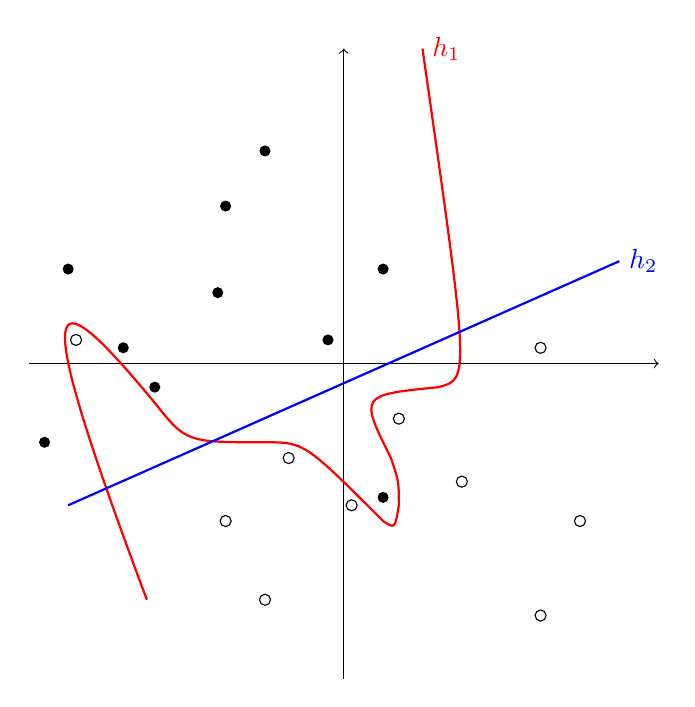
\begin{tikzpicture}
  \draw [->] (-4,0) -- (4,0);
  \draw [->] (0,-4) -- (0,4);
  \draw[red,thick] (-2.5,-3) .. controls (-4,1) and (-3.8,1.2) .. (-2.4,-.5)
    .. controls (-2,-1) .. (-1,-1) .. controls (-.5,-1) ..  (.5,-2)
    .. controls (.65, -2.1) .. (.7,-1.8) .. controls (.7,-1.5)
    ..  (.6,-1.2) .. controls (.2,-.4) .. (1.2, -.3)
    .. controls (1.6,-.2) .. (1,4);

  \foreach \Point in {(-3.4, .3), (2.5, .2), (-1.5,-2), (-1,-3),(.7,-.7),
    (3, -2), (2.5, -3.2), (-.7,-1.2), (0.1,-1.8), (1.5, -1.5)}{
    \draw \Point circle[radius=2pt];
  }
  \foreach \Point in {(.5,-1.7),(-.2,.3),(-2.8,.2),(-2.4,-.3),(-1,2.7),
    (-1.5, 2), (-1.6, .9), (-3.8,-1), (-3.5,1.2),(.5, 1.2)}{
  \fill \Point circle[radius=2pt];
  }
  \draw[blue, thick] (-3.5,-1.8) -- (3.5,1.3);
  \node[right,blue] at (3.5,1.3) {$h_2$};
  \node[below,right,red] at (1,4) {$h_1$};

\end{tikzpicture}
\end{center}

A common strategy for specifying a \emph{regularizer} is to use the form
\[ R(\Theta) = \norm{\Theta - \Theta_{\it prior}}^2 \]
when we have some idea in advance that $\theta$ ought to be near some
value $\Theta_{\it prior}$.  
\note{Learn about Bayesian methods in machine learning to see the
  theory behind this and cool results!}
In the absence of such knowledge a default is
to {\em regularize toward zero}:
\[ R(\Theta) = \norm{\Theta}^2\;\;. \]

\section{Maximizing the margin}
One criterion to use for judging separators that classify all
examples correctly (that is, that have a 0-1 loss value of 0) is to
prefer ones that have a {\em large margin}.
Recall that the margin of a labeled point $(x,y)$
with respect to the hyperplane $\theta, \theta_0$ is
\[ \gamma(x,y,\theta,\theta_0) = \frac{y\left(\theta^Tx+\theta_0\right)}
{\norm{\theta}} \;\;.\]
The margin is positive if a point is classified correctly, and the
absolute value of the margin is the perpendicular distance of $x$ to the
hyperplane. The margin of a dataset $\data$ with respect to
$\theta,\theta_0$ is
\[ 
  \min_{(\ex{x}{i},\ex{y}{i})\in \data}
  \gamma(\ex{x}{i},\ex{y}{i},\theta,\theta_0)\;\;.
\]
The figure below illustrates the margin of two linear separators, each
with 0 loss, with respect to the same data set.  The separator, $h_1$,
with the larger margin $\gamma_1$ feels intuitively like it will have
better generalization performance.  Separator $h_2$ has a very small
margin and would make errors if the data were perturbed by a small
amount.  \note{There is a lot of interesting theoretical work
  justifying a preference for separators with large margin.  There is
  an important class of algorithms called {\it support vector
    machines} that focus on finding large-margin separators with some
  other interesting properties.  Before the current boom in neural
  networks, they were the ``go-to'' algorithms for classification.  We
  don't have time to study them in more detail in this class, but we
  recommend that you read about them some time.}

\begin{center}
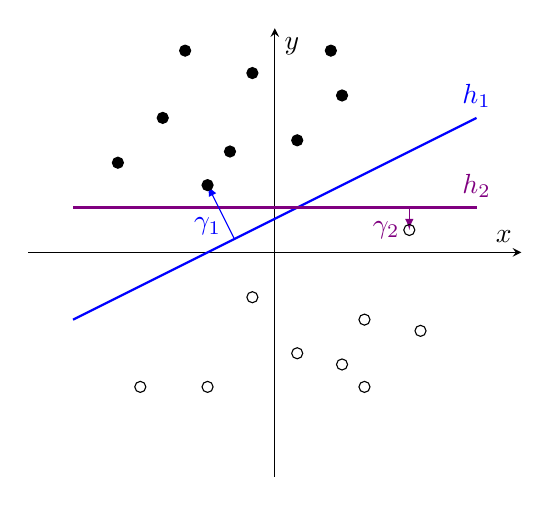
\begin{tikzpicture}
\begin{axis}[
    axis lines=middle, axis equal image,
    xmin=-11, xmax=11,
    ymin=-10, ymax=10,
    xtick=\empty, ytick=\empty,
    xlabel={$x$}, ylabel={$y$}
]
\addplot [only marks] table {
-3  3
1   5
-5  6
-1  8
3   7
-2  4.5
-7  4
-4  9
2.5 9
};
\addplot [only marks, mark=o] table {
-1  -2
-3  -6
4   -3
1   -4.5
3   -5
6   1
4   -6
6.5 -3.5
-6  -6
};
\addplot [domain=-9:9, samples=2, thick, blue] {.5*x+1.5} node[above] {$h_1$};
\addplot [domain=-9:9, samples=2, thick, violet] {2} node[above] {$h_2$};
\draw [latex-,blue] (axis cs: -3, 3) node [blue,yshift=-1.5em] {$\gamma_1$}
  -- (axis cs: -1.8, .6);
\draw [latex-,violet] (axis cs: 6, 1) node [violet,left] {$\gamma_2$}
  -- (axis cs: 6, 2);
\end{axis}
\end{tikzpicture}
\end{center}

If our data is linearly separable, we can frame the problem of finding
the maximum-margin separator as
\[
  \theta^*, \theta_0^* = \argmax{\theta,\theta_0} \min_i \gamma(\ex{x}{i},
  \ex{y}{i},\theta,\theta_0)\;\;,
\]
which we can find by minimizing the objective
\[
  J(\theta,\theta_0) = -\min_i \gamma(\ex{x}{i},\ex{y}{i},\theta,
  \theta_0)\;\;.
\]
However, this form of the objective can be tricky to optimize because
it is only sensitive to a single data point at a time, and so gradient
methods won't work very well.\note{This remark won't make sense to you
  until you understand more about gradient methods---so come back to
  think about it after you read the next chapter.}

We will develop another formulation.  Let's start by assuming
that we can guess what a good target value would be for the margin,
and call it $\gamma_{\it ref} > 0$. We can then set up a problem in
which we try to find a separator with margin $\gamma_{\it ref}$.
Ultimately, our goal will be to find a value for $\gamma_{\it ref}$
and a separator such that:
\begin{itemize}
  \item all points have margin $> \gamma_{\it ref}$ and
  \item the target margin $\gamma_{\it ref}$ is big.
\end{itemize}

\noindent To make this more precise, we start by defining a new loss function
\note{Confusion alert:  we have told you that loss functions are a
  function of two arguments, a guessed value and an actual value, but
  this ``loss function'' has a single argument, which is a margin.  A
  margin already combines the guess
  $\theta^Tx+\theta_0 / \norm{\theta}$ with the actual value
  $y$.  This is a standard way of framing the problem in the ML world,
  so we will stick with it.}
called the {\em hinge loss}:
\[
  L_h (\gamma / \gamma_{\it ref}) =
    \begin{cases}
      1 - \gamma / \gamma_{\it ref} & \text{ if } \gamma < \gamma_{\it ref} \\
      0 & \text{ otherwise}
    \end{cases}\;\;.
\]
The figure below and to the left plots the hinge loss as a function of
the margin, $\gamma$, of a point.  It is zero if the margin is greater
than $\gamma_{\it ref}$ and increases linearly as the margin decreases
(because we {\em really} want the margin to be bigger than
$\gamma_{\it ref}$!).
\begin{center}
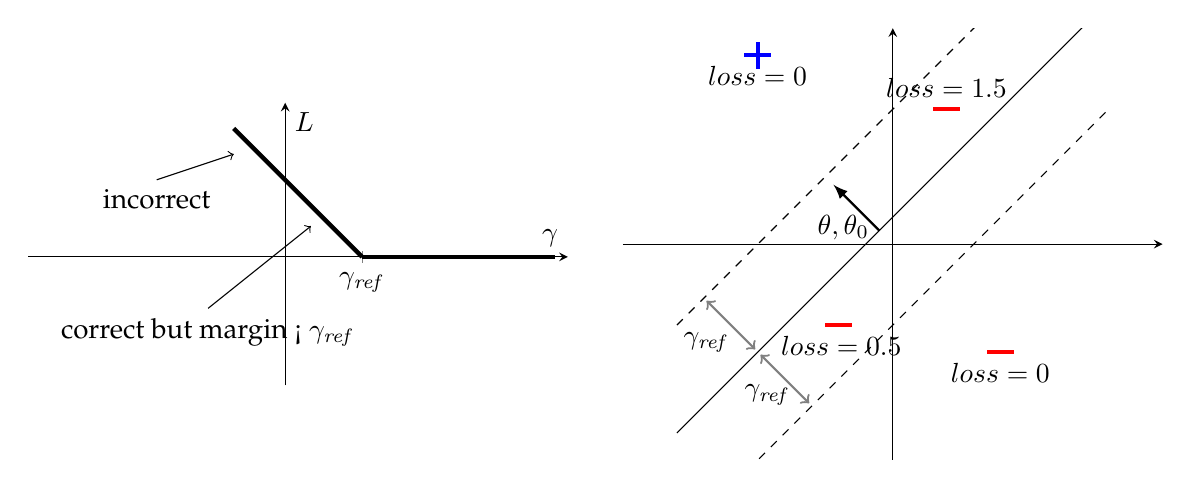
\begin{tikzpicture}
\begin{axis}[
    name=left,
    axis lines=middle, axis equal image,
    xmin=-10, xmax=11,
    ymin=-5, ymax=6,
    xtick={3}, ytick=\empty,
    xticklabels={$\gamma_{\it ref}$},
    xlabel={$\gamma$}, ylabel={$L$},
]
\addplot [domain=-2:3, samples=2, ultra thick] {3-x}; 
\addplot [domain=3:10.5, samples=2, ultra thick] {0};
\draw [->] (axis cs: -5, 3) node [black,below] {incorrect}
  -- (axis cs: -2, 4);
\draw [->] (axis cs: -3, -2) node [black,below] {correct but
  margin < $\gamma_{\it ref}$}
  -- (axis cs: 1, 1.2);

\end{axis}
\begin{axis}[
    axis lines=middle, axis equal image,
    xmin=-10, xmax=10,
    ymin=-8, ymax=8,
    xtick=\empty, ytick=\empty,
    at = (left.east), anchor = west, xshift = .7cm
]
\addplot [domain=-8:8, samples=2] {x+1}; 
\addplot [domain=-8:8, samples=2,dashed] {x+5};
\addplot [domain=-8:8, samples=2,dashed] {x-3};
\draw [thick,-latex] (axis cs: -0.5, 0.5) node [black,left,yshift=.1em]
  {$\theta,\theta_0$} -- (axis cs: -2.2, 2.2) ;
  
  \draw[ultra thick, blue] +(axis cs: -5-.5,7) -- +(axis cs: -5+.5,7)
    node [black,below,xshift=-.5em] {$loss=0$};
  \draw[ultra thick, blue] +(axis cs: -5,7-.5) -- +(axis cs: -5,7+.5);

  \draw[ultra thick, red] +(axis cs: 2-.5,5) -- +(axis cs: 2+.5,5)
    node [black,above,xshift=-.5em] {$loss=1.5$};
  \draw[ultra thick, red] +(axis cs: -2-.5,-3) -- +(axis cs: -2+.5,-3)
    node [black,below,xshift=-.4em] {$loss=0.5$};
  \draw[ultra thick, red] +(axis cs: 4-.5,-4) -- +(axis cs: 4+.5,-4)
    node [black,below,xshift=-.5em] {$loss=0$};

  \draw[<->, gray, thick] (axis cs: -5.1,-3.9) -- (axis cs: -6.9, -2.1)
    node [black,yshift=-1.5em] {$\gamma_{\it ref}$};
  \draw[<->, gray, thick] (axis cs: -4.9,-4.1) -- (axis cs: -3.1, -5.9)
    node [black,yshift=.3em,xshift=-1.5em] {$\gamma_{\it ref}$};
\end{axis}
\end{tikzpicture}
\end{center}

\question{Plot 0-1 loss on the axes of the figure on the left.}

In the figure on the right, we illustrate a hyperplane $\theta, \theta_0$.
Parallel to that hyperplane, but offset in either direction by
$\gamma_{\it ref}$ are two more hyperplanes (dotted lines in the
figure) representing the margins.  Any correctly classified point
outside the margin has loss 0.  Any correctly classified point inside
the margin has loss in $(0, 1)$.  Any incorrectly classified point has
loss $\geq 1$.  
\question{Be sure you can compute the loss values shown on this
  figure.  Also, try to visualize a plot in 3 dimensions that shows
  the loss function for positive points and the loss function for
  negative points going in the $Z$ dimension (up out of the page) on
  top of this plot.}

Now, let's formulate an objective function, in terms of the parameters
$\Theta = (\theta, \theta_0, \gamma_{\it ref})$.  
We will express our desire for a large margin by employing a regularization 
term in the objective function, namely
$R(\theta,\theta_0, \gamma_{\it ref}) = 1/\gamma_{\it 
    ref}^2$. \note{If you are thinking to yourself that we could
  express the desire for large margin by setting $R = -\gamma_{\it ref}$ or $R =
  1/\gamma_{\it ref}$ or any of a variety of other things, you would be right.
  We'll insist on this choice for now, because it will turn out to
  have useful consequences later, but you have no way of seeing that
  at this point.}
Then, we have 
\[
  J(\theta,\theta_0,\gamma_{\it ref}) = \frac{1}{n}\sum_{i=1}^n
  L_h\left(\frac{\gamma(\ex{x}{i},\ex{y}{i},\theta,\theta_0)}{\gamma_{\it ref}}
  \right) + \lambda\left(\frac{1}{\gamma_{\it ref}^2}\right)\;\;.
\]
We see that the two terms in the objective function have opposing
effects, favoring small and large $\gamma_{\it ref}$, respectively,
with $\lambda$ \note{Because it's not a parameter of the hypothesis,
  but rather a parameter of the method we are using to choose the
  hypothesis, we call $\lambda$ a {\em hyperparameter.}}  governing
the trade-off.  
\question{ You should, by now, be asking yourself
  ``How do we pick $\lambda$?''  You can think of the different
  objective functions that result from different choices of
  hyperparameter $\lambda$ as different {\em learning algorithms}.
  What do you know about choosing among algorithms?  How would you use
  that to pick $\lambda$?
}

Now, in order to slightly simplify our problem and to connect up with
more standard existing methods, we are going to make a somewhat
unintuitive step.  \note{This is kind of tricky.  Stew about it until
  it  makes sense to you.}
We actually have one more parameter in our set of parameters
$(\theta, \theta_0, \gamma_{\it ref})$ than is really necessary for
describing our hypothesis and objective, so we are going to rewrite it.

Remember that any linear scaling of $\theta,\theta_0$
represents the same separator.  So, without losing any ability to
represent separators or describe their margins, 
we can scale $\theta, \theta_0$ so that 
\[ \norm{\theta} = \frac{1}{\gamma_{\it ref}}\;\;. \]
\note{It's like we're secretly encoding our target margin as the
  inverse of the norm
  of $\theta$.}
Note that, because our target margin scales inversely with
$\norm{\theta}$, wanting the margin to be large is the same as wanting
$\norm{\theta}$ to be small.

With this trick, we don't need $\gamma_{\it ref}$ as a parameter any
more, and we get the following objective, which is the objective
  for support vector machines, and we'll often refer to as the 
SVM objective:
\[ J(\theta,\theta_0) = \left(\frac{1}{n}\sum_{i=1}^n L_h\left(\ex{y}{i}
(\theta^Tx+\theta_0)\right)\right) + \lambda\norm{\theta}^2 \;\;.\]
For any linearly separable data set, here are some observations:
\begin{enumerate}
  \item If $\lambda = 0$, $\theta, \theta_0$ can always
    be chosen so that the objective function evaluates to 0.
  \item If $\lambda > 0$ but is very small, we will pick $\theta$
    with smallest $\norm{\theta}$ while still maintaining separation
    of the data.
  \item If $\lambda$ is large, we tolerate errors in favor of having a
    ``simpler'' (smaller norm) separator.
\end{enumerate}
\question{Be sure you can make a detailed explanation of each of these
  points.   In point 1 above, would we need to increase or decrease the
  magnitude of $\theta$ to make the objective go to zero?  How does
  point 3 relate to the idea of regularizing toward zero?}

At the optimum, for separable data with very small $\lambda$:
\begin{itemize}
  \item $\ex{y}{i}\left(\theta^T\ex{x}{i} + \theta_0\right) \geq 1$ for
  all $i$, so as to keep the hinge loss to 0 for all points.
  \item $\ex{y}{i}\left(\theta^T\ex{x}{i} + \theta_0\right) = 1$ for
  at least one $i$, because the regularizer will drive $\norm{\theta}$ to be
  as small as possible with the loss still remaining at 0. 
\end{itemize}
To understand this, we note that
points for which $\ex{y}{i}\left(\theta^T\ex{x}{i} + \theta_0\right) = 1$
have margin exactly equal to $\gamma_\text{ref}$ (otherwise we could decrease
  $\norm{\theta}$ to obtain a larger margin). For these points that lie
  along the margin, we use the signed distance from $\theta,\theta_0$ to the point to
  compute the margin of this separator with respect to the data set:
  \[ \frac{\ex{y}{i}\left(\theta^T\ex{x}{i}+\theta_0\right)}
    {\norm{\theta}} = \text{margin}\;\;,\]
and so 
 \[\text{margin} =\frac{1}{\norm{\theta}} \;\;.\]

\note{Note that this last assertion (that the margin is the inverse of
  the norm of $\theta$) is only true under the assumptions listed at
  the top of this paragraph:  when the data is separable, when
  $\lambda$ is very small, and when $\theta$ is the optimum of the SVM
  objective.}  
\question{Be sure you can derive this last step and understand the
  conditions under which it holds!}


%%% Local Variables:
%%% mode: latex
%%% TeX-master: "top"
%%% End:

%\chapter{Linear classifiers}
\label{chap-classification}

%%%%%%%%%%%%%%%%%%%%%%%%%%%%%%%%%%%%%%%%%%%%%%%%%%%%%%%%%%%%%%%%%%%%%%%%%%%%%
\section{Classification}

A binary {\em{classifier}} is  \anchorednote{a mapping from $\R^d \rightarrow \{-1, +1\}$.}{Actually,
  general classifiers can have a range which is any discrete set, but we'll
  work with this specific case for a while.}  We'll often use the
letter $h$ (for hypothesis) to stand for a classifier, so
the classification process looks like:
$$ x \rightarrow \boxed{h} \rightarrow y \;\;.$$

Real life rarely gives us vectors of real numbers;  the $x$ we really
want to classify is usually something like  a song, image, or person.
In that case, we'll have to define a function $\varphi(x)$, whose
domain is $\R^d$, where $\varphi$ represents
  {\em features} of $x$, like a person's height or the amount of bass in
a song, and then let the $h: \varphi(x) \rightarrow \{-1, +1\}$.
In much of the following, we'll omit explicit mention of $\varphi$ and
assume that the $\ex{x}{i}$ are in $\R^d$, but you should always have
in mind that some additional process was almost surely required to go
from the actual input examples to their feature representation.

In {\em{supervised learning}} we are given a training data set of the
form
\[ \data_n = \left\{\left(\ex{x}{1}, \ex{y}{1}\right), \dots, \left(\ex{x}{n},
  \ex{y}{n}\right)\right\} \;\;.\]
We will assume that each $\ex{x}{i}$ is a $d \times 1$ {\em column
    vector}. The intended meaning of this data is that, when given an input
$\ex{x}{i}$, the learned hypothesis should generate output
$\ex{y}{i}$.

What makes a classifier useful? That it works well on {\em new} data;
that is, that it makes good predictions on \anchorednote{examples it hasn't
  seen.}{My favorite analogy is to problem sets.  We evaluate a
  student's ability to {\em generalize} by putting questions on
  the exam that were not on the homework (training set).}
But we don't know exactly what data this classifier might be tested on
when we use it in the real world. So, we have to {\em{assume}} a
connection between the training data and testing data; typically, they
are drawn independently from the same probability distribution.

Given a training set $\data_n$ and a classifier $h$, we can define the
  {\em{training error}} of $h$ to be
\begin{eqnarray*}
  \trainerr(h) = \frac{1}{n}\sum_{i = 1}^{n}\begin{cases} 1 &
              h(\ex{x}{i}) \ne \ex{y}{i} \\ 0 & \text{otherwise}\end{cases}
  \;\;.
\end{eqnarray*}

For now, we will try to find a classifier with small training error
(later, with some added criteria) and hope it {\em{generalizes well}}
to new data, and has a small {\em test error}
\begin{eqnarray*}
  \mathcal{E}(h) = \frac{1}{n'}\sum_{i = n + 1}^{n + n'}\begin{cases}
    1 & h(x^{(i)}) \ne y^{(i)} \\ 0 & \text{otherwise}\end{cases}
\end{eqnarray*}
on $n'$ new examples that were not used in the process of finding the
classifier.

%%%%%%%%%%%%%%%%%%%%%%%%%%%%%%%%%%%%%%%%%%%%%%%%%%%%%%%%%%%%%%%%%%%%%%%%%%%%%
\section{Learning algorithm}
A {\em hypothesis class} $\hclass$ is a set (finite or infinite) of
possible classifiers, each of which represents a mapping from
$\R^d \rightarrow \{-1, +1\}$.

A {\em learning algorithm} is a
procedure that takes a data set $\data_n$ as input and returns an
element $h$ of $\hclass$;  it looks  like
\begin{equation*}
  \data_n \longrightarrow \boxed{\text{learning alg ($\hclass$)}} \longrightarrow h
\end{equation*}

We will find that the choice of $\hclass$ can have a big impact on the
test error of the $h$ that results from this process.
One way to get $h$ that generalizes well is to restrict the size, or
``expressiveness'' of $\hclass$.

%%%%%%%%%%%%%%%%%%%%%%%%%%%%%%%%%%%%%%%%%%%%%%%%%%%%%%%%%%%%%%%%%%%%%%%%%%%%%
\section{Linear classifiers}

We'll start with the hypothesis class of {\em linear classifiers}.
They are (relatively) easy to understand, simple in a mathematical
sense, powerful on their own, and the basis for many other more
sophisticated methods.

A linear classifier in $d$ dimensions is
defined by a vector of parameters $\theta \in \R^d$ and scalar
$\theta_0 \in \R$.  So, the hypothesis class $\hclass$ of linear
classifiers in $d$ dimensions is the {\em set} of all vectors in
$\R^{d+1}$.   We'll assume that $\theta$ is a $d \times 1$ column
vector.

Given particular values for $\theta$ and $\theta_0$, the  \anchorednote{classifier is
  defined by}{Let's be careful about dimensions.  We have assumed that $x$ and
  $\theta$ are both $d \times 1$ column vectors.  So $\theta^T x$ is $1
    \times 1$, which in math (but not necessarily numpy) is the same as a
  scalar.}
\begin{eqnarray*}
  h(x; \theta, \theta_0) = \text{sign}(\theta^T x + \theta_0)
  = \begin{cases} +1 & \text{if $\theta^Tx + \theta_0 > 0$} \\ -1 &
              \text{otherwise}\end{cases} \;\;.
\end{eqnarray*}
Remember that we can think of $\theta, \theta_0$ as specifying a
hyperplane.  It divides $\R^d$, the space our $\ex{x}{i}$ points live
in, into two half-spaces.  The one that is on the same side as the
normal vector is the {\em positive} half-space, and we classify all
points in that space as positive.  The half-space on the other side is
  {\em negative} and all points in it are classified as negative.

\begin{examplebox}{\bf Example:}
  Let $h$ be the linear classifier defined by
  $\theta = \protect\twodcol{-1}{1.5}, \theta_0 = 3$.

  \noindent The diagram below shows several points classified by $h$.
  In particular, let $\ex{x}{1} = \twodcol{3}{2}$ and
  $\ex{x}{2} = \twodcol{4}{-1}$.
  \begin{align*}
    h(\ex{x}{1}; \theta, \theta_0) & = \sign\left(\twodrow{-1}{1.5}\twodcol{3}{2} + 3\right) = \sign(3) = +1     \\
    h(\ex{x}{2}; \theta, \theta_0) & = \sign\left(\twodrow{-1}{1.5}\twodcol{4}{-1} + 3\right) = \sign(-2.5) = -1
  \end{align*}
  Thus, $\ex{x}{1}$ and $\ex{x}{2}$ are given positive and negative classfications,
  respectively.

  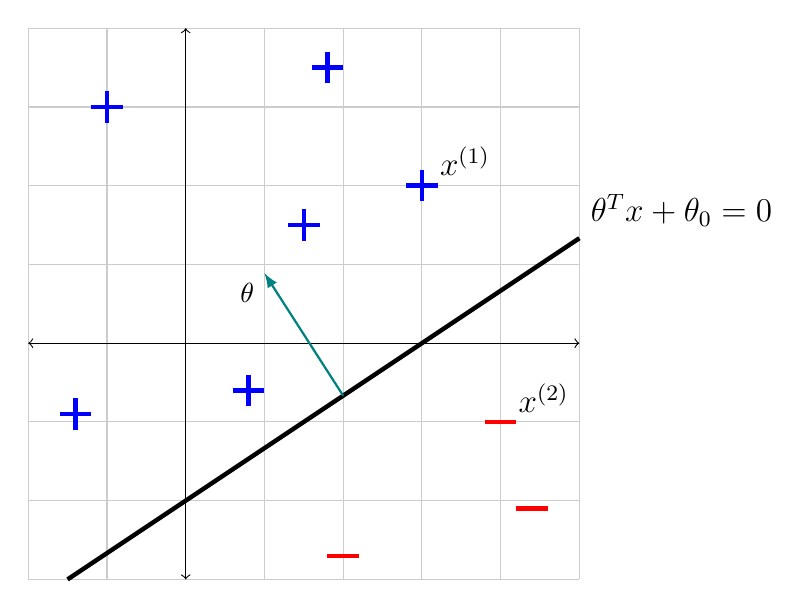
\begin{tikzpicture}
    \draw [thin, gray!40] (-2,-3) grid (5,4);
    \draw [<->] (-2,0) -- (5,0);
    \draw [<->] (0,-3) -- (0,4);

    \draw [ultra thick] (-1.5,-3) -- (5,1.3333)
    node [above right] {\large$\theta^Tx + \theta_0 = 0$};

    \draw [thick,teal,-latex] (2,-0.6667) -- (1,0.8883)
    node [black,below left] {$\theta$};

    \node [above right,xshift=.3em] at (3,2) {\large$\ex{x}{1}$};
    \node [above right,xshift=.3em] at (4,-1) {\large$\ex{x}{2}$};


    \foreach \Point in {(3,2), (1.8,3.5), (-1,3), (.8,-.6), (-1.4,-.9),
        (1.5, 1.5)}{
        \pic at \Point {plus};
      }

    \foreach \Point in {(4,-1), (2,-2.7), (4.4,-2.1)}{
        \pic at \Point {minus};
      }
  \end{tikzpicture}

\end{examplebox}

\question{What is the green vector normal to the hyperplane?  Specify it
  as a column vector.}
\question{
  What change would you have to make to $\theta, \theta_0$ if you wanted
  to have the separating hyperplane in the same place, but to classify
  all the points labeled '+' in the diagram as negative and all the
  points labeled '-' in the diagram as positive?}

%%%%%%%%%%%%%%%%%%%%%%%%%%%%%%%%%%%%%%%%%%%%%%%%%%%%%%%%%%%%%%%%%%%%%%%%%%%%%
\section{Learning linear classifiers}

Now, given a data set and the hypothesis class of linear classifiers,
our objective will be to find the linear classifier with the smallest
possible training error.
  %This strategy is (mostly) okay because the
  %class of linear classifiers is, in some sense, small.

  {\em This is a well-formed optimization problem. But it's not
    computationally easy!}

We'll start by considering a very simple learning algorithm. \note{It's
  a good idea to think of the ``stupidest possible'' solution to a
  problem, before trying to get clever.  Here's a fairly (but not
  completely) stupid algorithm.}  The idea is to generate $k$ possible
hypotheses by generating their parameter vectors at random.  Then, we
can evaluate the training-set error on each of the hypotheses and
return the hypothesis that has the lowest training error (breaking
ties arbitrarily).

\begin{codebox}
  \Procname{$\proc{Random-Linear-Classifier}(\dataTrain, k)$}
  \li \For $j \gets 1$ \To $k$
  \li   \Do
  randomly sample $\left(\ex{\theta}{j},
    \ex{\theta_0}{j}\right)$ from $(\R^d, \R)$
  \End
  \li $j^* \gets \argmin{j \in \{1, \ldots, k\}} \mathcal{E}_n \left(\ex{\theta}{j}, \ex{\theta_0}{j}\right)$
  \li \Return $\left(\ex{\theta}{j^*}, \ex{\theta_0}{j^*}\right)$
\end{codebox}



A note about terminology and
\anchorednote{notation.}
{The notation within the algorithm above might be new to you:
  $\argmin{x} f(x)$
  means the value of $x$ for which $f(x)$ is the smallest.  Sometimes
  we write $\argmin{x \in {\cal X}} f(x)$ when we want to explicitly
  specify the set ${\cal X}$ of values of $x$ over which we want to
  minimize.}
The training data $\dataTrain$ is an input to the learning algorithm,
and the output of this learning algorithm will be a hypothesis $h$, where
$h$ has parameters $\theta$ and $\theta_{0}.$
In contrast to $\theta$ and $\theta_{0}$, the input $k$ is a
parameter of the learning algorithm itself; such
parameters are often called {\em hyperparameters}.

\question{
  What do you think will be observed for $\trainerr(h)$, where $h$ is the
  hypothesis returned by \proc{Random-Linear-Classifier}, if this learning
  algorithm is run multiple times? And as $k$ is increased? }

\question{
  What properties of $\dataTrain$ do you think will have an
  effect on $\trainerr(h)$?
}

%%%%%%%%%%%%%%%%%%%%%%%%%%%%%%%%%%%%%%%%%%%%%%%%%%%%%%%%%%%%%%%%%%%%%%%%%%%%%
\section{Evaluating a learning algorithm}
How should we evaluate the performance of a {\em classifier} $h$?   The best
method is to measure {\em test error} on data that was not used to
train it.

How should we evaluate the performance of a {\em learning algorithm}?
This is trickier.  There are many potential sources of variability in
the possible result of computing test error on a learned hypothesis $h$:
\begin{itemize}
  \item Which particular {\em training examples} occurred in $\dataTrain$
  \item Which particular {\em testing examples} occurred in $\dataTest$
  \item Randomization inside the learning {\em algorithm} itself
\end{itemize}
Generally, we would like to execute the following process multiple
times:
\begin{itemize}
  \item Train on a new training set
  \item Evaluate resulting $h$ on a testing set {\em that does not
            overlap the training set}
\end{itemize}
Doing this multiple times controls for possible poor choices of
training set or unfortunate randomization inside the algorithm itself.

One concern is that we might need a lot of data to do this, and in
many applications data is expensive or difficult to acquire. We can
re-use data with {\em{cross validation}} (but it's harder to do theoretical
analysis).  \\
\begin{codebox}
  \Procname{$\proc{Cross-Validate}(\data, k)$}
  \li divide $\data$ into $k$ chunks $\data_1, \data_2, \ldots \data_k$ (of roughly equal size)
  \li \For $i \gets 1$ \To $k$
  \li   \Do
  train $h_i$ on $\data \setminus \data_i$ (withholding chunk $\data_i$)
  \li     compute ``test'' error $\mathcal{E}_i (h_i)$ on withheld data $\data_i$
  \End
  \li \Return $\frac{1}{k} \sum_{i=1}^k \mathcal{E}_i (h_i)$
\end{codebox}

It's very important to understand that cross-validation neither
delivers nor evaluates a single particular hypothesis $h$.  It
evaluates the {\em algorithm} that produces hypotheses.

%%%%%%%%%%%%%%%%%%%%%%%%%%%%%%%%%%%%%%%%%%%%%%%%%%%%%%%%%%%%%%%%%%%%%%%%%%%%%
\section{Feature representation for classifiers}

Linear classifiers are easy to work with and analyze, but they are a
very restricted class of hypotheses.  If we have to make a complex
distinction in low dimensions, then they are unhelpful.

Our favorite illustrative example is the ``exclusive or'' ({\sc xor})
data set, the drosophila \note{D. Melanogaster is a species of fruit
  fly, used as a simple system in which to study genetics, since 1910.}
of machine-learning data sets:

\begin{examplebox}
  \begin{center}
    \begin{tikzpicture}
      \pic at (-1, -1) {plusblk};
      \pic at (-1, +1) {minusblk};
      \pic at (+1, -1) {minusblk};
      \pic at (+1, +1) {plusblk};
    \end{tikzpicture}
  \end{center}
\end{examplebox}

There is no linear separator for this two-dimensional dataset!  But, we have a trick
available:  take a low-dimensional data set and move it, using a
non-linear transformation into a higher-dimensional space, and look
for a linear separator there. Let's look at an example data set that
starts in 1-D:

\begin{examplebox}
  \begin{center}
    \begin{tikzpicture}
      \draw [<->, gray] (-3,0) -- (3,0)
      node [black, right] {$x$};
      \draw [gray] (0,.6) -- (0,-.6)
      node [black, below] {0};

      \pic at (-1.5, 0) {plusblk};
      \pic at (-.5, 0) {minusblk};
      \pic at (.5, 0) {minusblk};
      \pic at (1.5, 0) {plusblk};

    \end{tikzpicture}
  \end{center}
\end{examplebox}

These points are not linearly separable, \note{What's a linear
  separator for data in 1D?  A point!}  but consider the
transformation $\phi(x) = [x,x^2]$. Putting the data in $\phi$ space,
we see that it is now separable.  There are lots of possible
separators;  we have just shown one of them here.

\begin{examplebox}
  \begin{center}
    \begin{tikzpicture}
      \draw [<->, gray] (-3,0) -- (3,0)
      node [black, right] {$x$};
      \draw [<->, gray] (0,-.6) -- (0,4)
      node [black, above] {$x^2$};

      \draw [dashed] (-3, 1.25) -- (3, 1.25)
      node [below, xshift=-1cm] {separator};

      \pic at (-1.5, 2.25) {plusblk};
      \pic at (-.5, .25) {minusblk};
      \pic at (.5, .25) {minusblk};
      \pic at (1.5, 2.25) {plusblk};

    \end{tikzpicture}
  \end{center}
\end{examplebox}

A linear separator in $\phi$ space is a nonlinear separator in the
original space!  Let's see how this plays out in our simple example.
Consider the separator $x^2  - 1 = 0$, which labels the half-plane
$x^2 -1 > 0$ as positive.  What separator does it correspond to in the
original 1-D space?
We have to ask the question:  which $x$ values have the property that
$x^2 - 1 = 0$.  The answer is $+1$ and $-1$, so those two points
constitute our separator, back in the original space.  And we can use
the same reasoning to find the region of 1D space that is labeled
positive by this separator.

\begin{examplebox}
  \begin{center}
    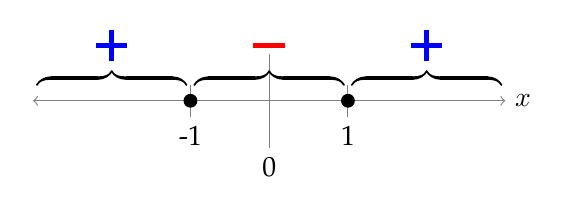
\begin{tikzpicture}
      \draw [<->, gray] (-3,0) -- (3,0)
      node [black, right] {$x$};
      \draw [gray] (0,.6) -- (0,-.6)
      node [black, below] {0};
      \draw [gray] (1,.2) -- (1,-.2)
      node [black, below] {1};
      \draw [gray] (-1,.2) -- (-1,-.2)
      node [black, below] {-1};

      \fill (1,0) circle (2.5pt);
      \fill (-1,0) circle (2.5pt);

      \draw[decoration={calligraphic brace,amplitude=5pt}, decorate, line width=1.25pt]
      (-2.95,0.2) node {} -- (-1.05,0.2);
      \draw[decoration={calligraphic brace,amplitude=5pt}, decorate, line width=1.25pt]
      (-.95,0.2) node {} -- (.95,0.2);
      \draw[decoration={calligraphic brace,amplitude=5pt}, decorate, line width=1.25pt]
      (1.05,0.2) node {} -- (2.95,0.2);

      \pic at (-2, 0.7) {plus};
      \pic at (0, 0.7) {minus};
      \pic at (2, 0.7) {plus};

    \end{tikzpicture}
  \end{center}
\end{examplebox}

This is a very general and widely useful strategy.  It's the basis for
  {\em kernel methods}, a powerful technique that we unfortunately won't
get to in this class, and can be seen as a motivation for multi-layer
neural networks.

%%%%%%%%%%%%%%%%%%%%%%%%%%%%%%%%%%%%%%%%
\subsection{Feature representation for XOR}

% FIXME: regenerate plots using optimization algorithm instead of perceptron

So, what if we try to solve the {\sc xor} problem using a polynomial
basis as the feature transformation?  We can just take our
two-dimensional data and transform it into a higher-dimensional data
set, by applying $\phi$.  Now, we have a classification problem as
usual, and we can use the perceptron algorithm to solve it.

Let's try it for $k = 2$ on our {\sc xor} problem.  The feature
transformation is
\[\phi((x_1, x_2)) = (1, x_1, x_2, x_1^2, x_1 x_2, x_2^2)\;\;.\]
\question{
  If we train a classifier after performing this feature
  transformation, would we lose any expressive
  power if we let $\theta_0 = 0$ (i.e. trained without offset instead of
  with offset)?}
After several iterations, we find a separator
with coefficients $\theta = (0, 0, 0, 0, 4, 0)$ and $\theta_0 =
  0$.
This corresponds to
\[0 + 0 x_1 + 0 x_2 + 0 x_1^2 + 4 x_1 x_2 + 0x_2^2 + 0 = 0\]
and is plotted below, with the gray shaded region classified as
negative and the white region classified as positive:
\begin{examplebox}
  \begin{center}
    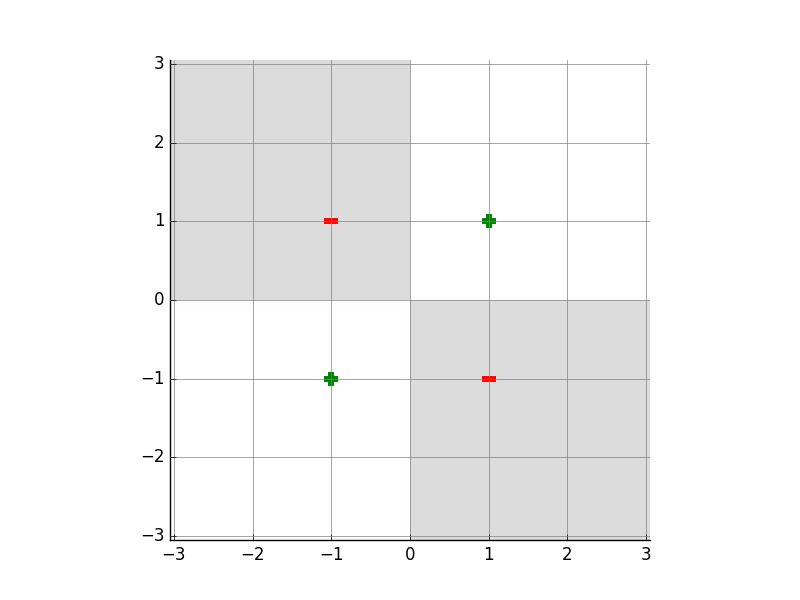
\includegraphics[scale=0.3]{figures/feature_representation_1.png}
  \end{center}
\end{examplebox}
\question{
  Be sure you understand why this high-dimensional hyperplane is a
  separator, and how it corresponds to the figure.}

For fun, we show some more plots below.  Here is the result of generating a linear classifier
on {\sc xor}, but where the data are put in a different
place on the plane: %  After 65 mistakes (!) it arrives at these coefficients:
$\theta = ( 1, -1, -1, -5, 11, -5)$, $\theta_0 =  1$, which generates
this separator:
\note{The jaggedness
  in the plotting of the separator is an artifact of a lazy lpk strategy
  for making these plots--the true curves are smooth.
}
\begin{examplebox}
  \begin{center}
    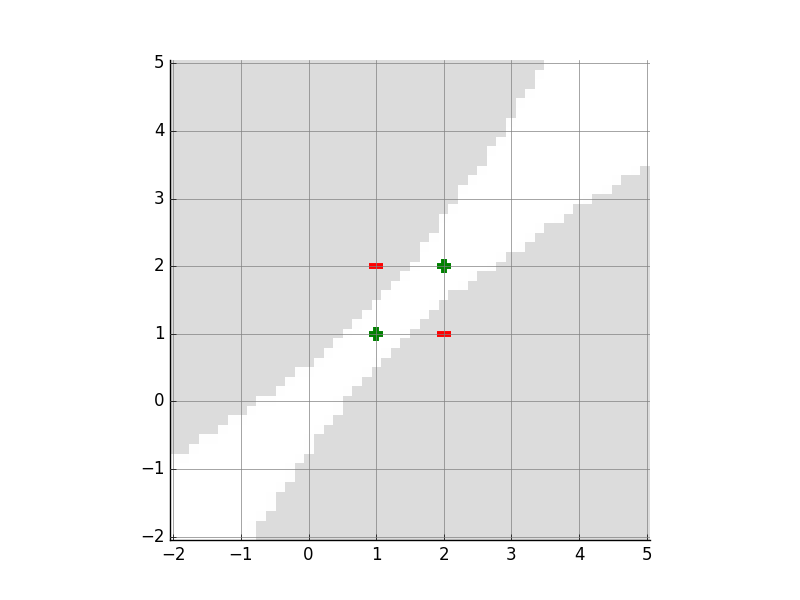
\includegraphics[scale=0.3]{figures/feature_representation_2.png}
  \end{center}
\end{examplebox}
\question{It takes many more iterations to solve this
  version.  Apply knowledge of the convergence properties of the
  perceptron to understand why.}

Here is a harder data set.  After 200 iterations, we could not		% FIXME: iterations of what?
separate it with a second or third-order basis representation.  Shown
below are the results after 200 iterations for bases of order 2, 3, 4,
and 5.
\begin{examplebox}
  \begin{center}
    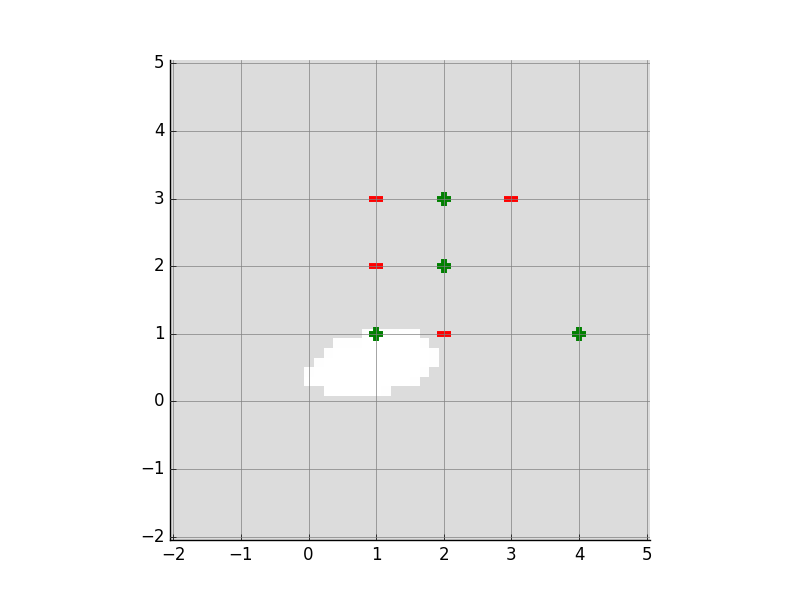
\includegraphics[width=0.48\linewidth]{figures/feature_representation_3.png}
    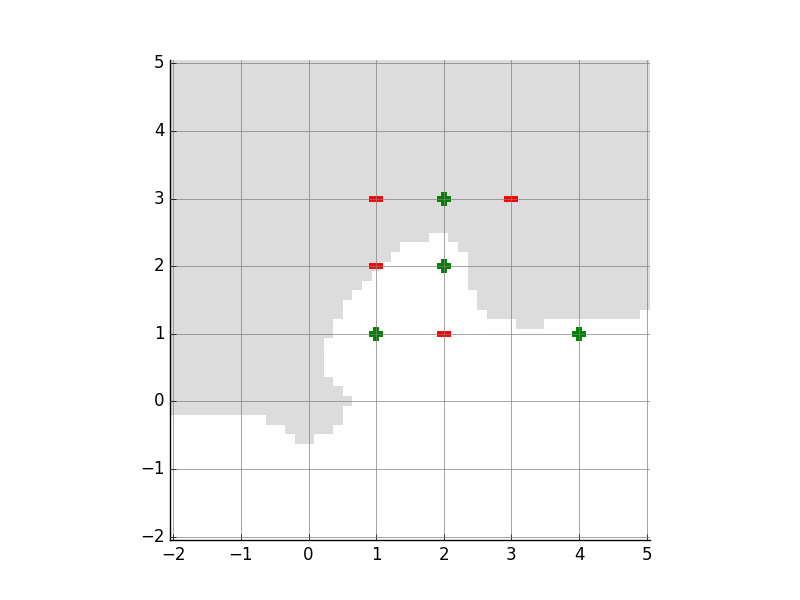
\includegraphics[width=0.48\linewidth]{figures/feature_representation_4.png} \\
    \includegraphics[width=0.48\linewidth]{figures/feature_representation_5.png}
    \includegraphics[width=0.48\linewidth]{figures/feature_representation_6.png}
  \end{center}
\end{examplebox}


%%% Local Variables:
%%% mode: latex
%%% TeX-master: "top"
%%% End:

%\chapter{Logistic regression}
\label{chap-logistic}


%%%%%%%%%%%%%%%%%%%%%%%%%%%%%%%%%%%%%%%%%%%%%%%%%%%%%%%%%%%%%%%%%%%%%%%%%%%%%
\section{A new hypothesis class: linear logistic classifiers}

For classification, it is natural to make predictions in $\{+1, -1\}$
and use the $0-1$ loss function.   However, even for simple linear
classifiers, it is very difficult to
find values for $\theta, \theta_0$ that minimize simple training error
\[J(\theta, \theta_0) = \frac{1}{n} \sum_{i=1}^n \mathcal{L}(\text{sign}(\theta^T\ex{x}{i} + \theta_0),
  \ex{y}{i})\;\;.\] This problem is NP-hard, which probably
\note{The ``probably'' here is not because we're too lazy to look it
  up, but actually because of a fundamental unsolved problem in
  computer-science theory, known as ``P vs. NP.''}
implies
that solving the most difficult instances of this problem would
require computation time {\em exponential} in the number of training
examples, $n$.

What makes this a difficult optimization problem is its lack of
``smoothness'':
\begin{itemize}
\item There can be two hypotheses, $(\theta, \theta_0)$  and
  $(\theta', \theta_0')$, where
  one is closer in parameter space to the optimal parameter values
  $(\theta^*, \theta_0^*)$, but they make the same number of
  misclassifications so they have the same $J$ value.
\item All predictions are categorical:  the classifier can't express a
  degree of certainty about whether a particular input $x$ should have
  an associated value $y$.
\end{itemize}
For these reasons, if we are considering a hypothesis $\theta,\theta_0$
that makes five incorrect predictions, it is difficult to see how we
might change $\theta,\theta_0$ so that it will perform better, which
makes it difficult to design an algorithm that searches through the
space of hypotheses for a good one.

For these reasons, we are going to investigate a new hypothesis class:
{\em linear logistic classifiers}.   These hypotheses are still
parameterized by a $d$-dimensional vector $\theta$ and a scalar
$\theta_0$, but instead of making predictions in $\{+1, -1\}$, they
generate real-valued outputs in the interval $(0, 1)$. A linear
logistic classifier has the form 
\[h(x; \theta, \theta_0) = \sigma(\theta^T x + \theta_0)\;\;.\]
This looks familiar!  What's new?

The {\em logistic} function, also known as the {\em sigmoid} function, 
is defined as
\[\sigma(z) = \frac{1}{1+e^{-z}}\;\;,\] and plotted below, as a
function of its input $z$.
Its output can be interpreted as a probability, because for any value of
$z$ the output is in $(0, 1)$.

\begin{center}
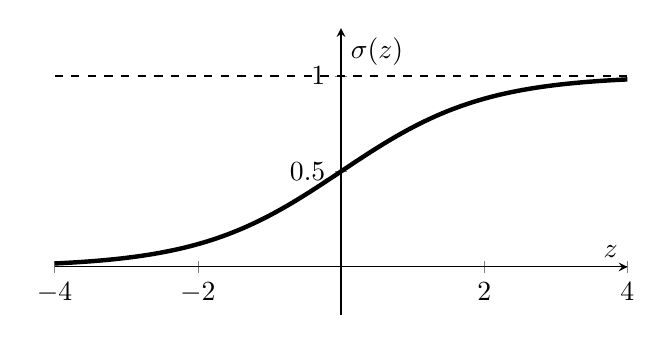
\begin{tikzpicture}
\begin{axis}[
  axis lines=middle,
  % axis equal image,
  scale only axis,
  width=0.6\textwidth,
  height=0.3\textwidth,
    xmin=-4, xmax=4,
    ymin=-0.25, ymax=1.25,
    xlabel={$z$}, ylabel={$\sigma(z)$},
]
\addplot [domain=-4:4, samples=100, ultra thick] {1/(1+exp(-x))};
\addplot [domain=-4:4, samples=2, dashed] {1};
\addplot [domain=-4:4, samples=2, dashed] {0};
\end{axis}
\end{tikzpicture}
\end{center}

\question{Convince yourself the output of $\sigma$ is always in the
  interval $(0, 1)$.  Why can't it equal 0 or equal 1?  For what value
of $z$ does $\sigma(z) = 0.5$?}

What does a linear logistic classifier (LLC) look like?   Let's consider the
simple case where $d = 1$, so our input points simply lie along the
$x$ axis.  The plot below shows LLCs for three different parameter
settings: $\sigma(10x + 1)$, $\sigma(-2x + 1)$, and $\sigma(2x - 3).$
\begin{center}
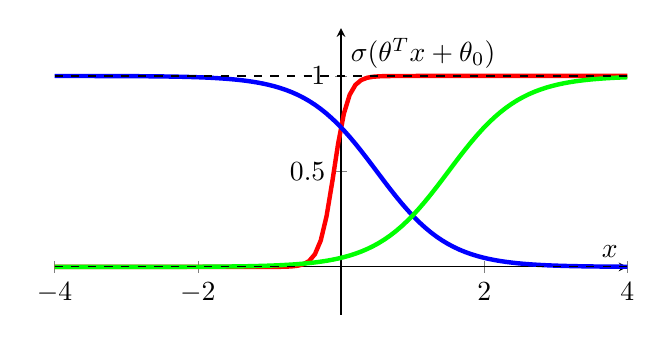
\begin{tikzpicture}
\begin{axis}[
  axis lines=middle,
  % axis equal image,
  scale only axis,
  width=0.6\textwidth,
  height=0.3\textwidth,
    xmin=-4, xmax=4,
    ymin=-0.25, ymax=1.25,
    xlabel={$x$}, ylabel={$\sigma(\theta^T x + \theta_0)$},
]
\addplot [domain=-4:4, samples=100, ultra thick, red] {1/(1+exp(-(10*x + 1)))};
\addplot [domain=-4:4, samples=100, ultra thick, blue] {1/(1+exp(-(-2*x
  + 1)))};
\addplot [domain=-4:4, samples=100, ultra thick, green] {1/(1+exp(-(2*x
  - 3)))};
\addplot [domain=-4:4, samples=2, dashed] {1};
\addplot [domain=-4:4, samples=2, dashed] {0};
\end{axis}
\end{tikzpicture}
\end{center}
\question{Which plot is which?  What governs the steepness of the
  curve?  What governs the $x$ value where the output is equal to
  0.5?}

But wait!  Remember that the definition of a classifier from
chapter~\ref{chap-classification} is that it's a mapping from $\R^d
\rightarrow \{-1, +1\}$ or to some other discrete set.  So, then, it
seems like an LLC is actually not a classifier! 

Given an LLC, with an output value in $(0, 1)$, what should we do if
we are forced to make a prediction in $\{+1, -1\}$?  A default answer
is to predict $+1$ if $\sigma(\theta^T x + \theta_0) > 0.5$ and $-1$
otherwise.  The value $0.5$ is sometimes called a {\em prediction
  threshold}.

In fact, for different problem settings, we might prefer to pick a
different prediction threshold.  The field of {\em decision theory}
considers how to make this choice from the perspective of Bayesian
reasoning.  For example, if the consequences of predicting $+1$ when
the answer should be $-1$ are much worse than the consequences of
predicting $-1$ when the answer should be $+1$, then we might set the
prediction threshold to be greater than $0.5$.

\question{Using a prediction threshold of 0.5, for what values of $x$
  do each of the LLCs shown in the figure above predict $+1$?}

When $d = 2$, then our inputs $x$ lie in a two-dimensional space with
axes $x_1$ and $x_2$, and the output of the LLC is a surface, as shown
below, for $\theta = (1, 1), \theta_0 = 2$.

\includegraphics[width=0.7\textwidth]{figures/logreg3d}

\question{Convince yourself that the set of points for which
  $\sigma(\theta^T x + \theta_0) = 0.5$, that is, the separator
  between positive and negative predictions with prediction threshold
  $0.5$ is a line in $(x_1, x_2)$ space. What particular line is it
  for the case in the figure above?
  How would the plot change for $\theta = (1, 1)$, but now
  with $\theta_0 = -2$? For $\theta = (-1, -1), \theta_0 = 2$?}

%%%%%%%%%%%%%%%%%%%%%%%%%%%%%%%%%%%%%%%%%%%%%%%%%%%%%%%%%%%%%%%%%%%%%%%%%%%%%
\section{Loss function for logistic classifiers}

\label{logistic}
Recall that optimization is a key approach to solving machine learning
problems; this also applies to logistic regression, as we can see by
defining a lass function for this problem.  Recall that a common loss function
is the 0-1 loss, introduced in Chapter~\ref{chap-intro}:
\[ L_{01}(h(x; \Theta), y) =
  \begin{cases}
    0 & \text{ if } y = h(x; \Theta)\\
    1 & \text{ otherwise}
  \end{cases}\;\;,
\]
which gives a value of 0 for a correct prediction, and a 1 for an
incorrect prediction.  In the case of linear separators, this becomes:
\[ L_{01}(h(x;\theta, \theta_0), y) =
  \begin{cases}
    0 & \text{ if } y(\theta^Tx + \theta_0) > 0 \\
    1 & \text{ otherwise}
  \end{cases}\;\;.
\]


%
For logistic regression, we have defined a class, LLC, of hypotheses whose outputs are in $(0, 1)$, 
but we have training data with $y$ values  in $\{+1, -1\}$.  How
can we define a loss function?  Intuitively, we would like to have
{\em low loss if we assign a low probability to the incorrect class.}
We'll define a loss function, called {\em negative log-likelihood} (NLL),
that does just this.  In  addition, it has the cool property that it
extends nicely to the case where we would like to classify our inputs
into more than two classes.

In order to simplify the description, we will assume that (or transform so that) the labels
in the training data are $y \in \{0, 1\}$, enabling them to be
interpreted as probabilities of being a member of the class of
interest.  \note{\bf Remember to be sure your $y$
  values have this form if you try to learn an LLC using NLL!|}
We would like to pick the parameters of our classifier to maximize the
probability assigned by the LCC to the correct $y$ values, as
specified in the training set.  Letting guess $\ex{g}{i} =
\sigma(\theta^T\ex{x}{i} + \theta_0)$, 
that probability is
\begin{equation*}
 \prod_{i = 1}^n \begin{cases} \ex{g}{i} & \text{if $\ex{y}{i} =
    1$}  \\ 1 - \ex{g}{i} & \text{otherwise}
\end{cases}\;\;,
\end{equation*}
under the assumption that our predictions are independent.  This can
be cleverly rewritten, when $\ex{y}{i} \in \{0, 1\}$, as
\begin{equation*}
 \prod_{i = 1}^n {\ex{g}{i}}^{\ex{y}{i}}(1 - \ex{g}{i})^{1 - \ex{y}{i}}\;\;.
\end{equation*}
\question{Be sure you can see why these two expressions are  the
  same.}

Now, because products are kind of hard to deal with, and because the
log function is monotonic, the $\theta, \theta_0$ that maximize the
log of this quantity will be the same  as the $\theta, \theta_0$ that
maximize the original, so we can try to maximize
\begin{equation*}
  \sum_{i = 1}^n  \left( {\ex{y}{i}}\log {\ex{g}{i}} +
            (1 - \ex{y}{i})\log(1 - \ex{g}{i})\right)\;\;. 
\end{equation*}
We can turn the maximization problem above into a minimization problem by taking the negative
of the above expression, and write in terms of minimizing a loss
\begin{equation*}
 \sum_{i = 1}^n \mathcal{L}_\text{nll}(\ex{g}{i}, \ex{y}{i})
\end{equation*}
where $\mathcal{L}_\text{nll}$ is the {\em negative log-likelihood}
loss function:
\begin{equation*}
\mathcal{L}_\text{nll}(\text{guess},\text{actual}) = 
-\left(\text{actual}\cdot \log (\text{guess}) + (1 - \text{actual})\cdot\log (1 -
  \text{guess})\right) \;\;.
\end{equation*}
This loss function is also sometimes referred to as the {\em log loss}
or {\em cross entropy}. \note{You can use any base for the logarithm
  and it won't make any real difference.  If we ask you for numbers,
  use log base $e$.}

\section{Logistic classification as optimization}

We can finally put all these pieces together and develop an objective
function for optimizing regularized negative log-likelihood for a
linear logistic classifier. \note{That's a lot of fancy words!}  In
  fact, this process is usually called ``logistic regression,'' so
  we'll call our objective $J_\text{lr}$, and define it as
\[J_\text{lr}(\theta, \theta_0; {\cal D}) =
  \left(\frac{1}{n} \sum_{i=1}^n
    \mathcal{L}_\text{nll}(\sigma(\theta^T \ex{x}{i} + \theta_0), \ex{y}{i})\right) +
     \lambda \norm{\theta}^2\;\;.\]
\question{Consider the case of linearly separable data.   What will
  the $\theta$ values that optimize this objective be like if
  $\lambda = 0$?   What will they be like if $\lambda$ is very big?
  Try to work out an example in one dimension with two data points.}

%%% Local Variables:
%%% mode: latex
%%% TeX-master: "top"
%%% End:
 old version
%\chapter{Recommender systems}
The problem of choosing items from a large set to recommend to a user
comes up in many contexts, including  music services, shopping, and online
advertisements.  As well as being an important application, it is
interesting because it has several formulations, some of which take
advantage of a particular interesting structure in the problem.

Concretely, we can think about a company like Netflix, which
recommends movies to its users.  Netflix knows the ratings given by
many different people to many different movies, and knows your ratings on a
small subset of all possible movies. How should it use this data to
recommend a movie for you to watch tonight?

There are two prevailing approaches to this problem.  The first,
{\em content-based recommendation}, is formulated as a supervised learning
problem.  The second, {\em collaborative filtering}, introduces a new
learning problem formulation.

\section{Content-based recommendations}
In content-based recommendation, we try to learn a predictor, $f$,
that uses the movies that you have rated so far as training data,
find a hypothesis that maps a movie into a prediction of what rating
you would give it, and then return some movies with high predicted
ratings.

The first step is designing representations for the input and output.

It's actually pretty difficult to design a good feature representation
for movies.   Reasonable approaches might construct features based on
the movie's genre, length,  main actors, director, location, or even
ratings given by some standard critics or aggregation sources.  This
design process would yield
\[\phi : \text{movie} \rightarrow \text{vector}\;\;.\]

Movie ratings are generally given in terms of some number of stars,
so the output domain might be \{1, 2, 3, 4, 5\}.  It's not
appropriate for one-hot encoding on the output, and pretending that
these are real values is also not entirely sensible.  Nevertheless, we
will treat the output as if it's in $\R$.
\note{Thermometer coding might be reasonable, but it's hard to say
  without trying it.  Some more advanced techniques try to predict
  rankings (would I prefer movie A over movie B) rather than raw
  ratings.}
\question{What is the disadvantage of using one-hot?
  What is the disadvantage of using $\R$?}

Now that we have an encoding, we can make a
training set based on {\em your} previous ratings of movies. Here,
$\ex{x}{i}$ represents the $i$th movie, $\phi(\ex{x}{i})$ gives our
feature representation of the $i$th movie, and $\ex{y}{i} = \text{rating}(\ex{x}{i})$
is your rating for the $i$th movie. If we let $J = \{1,2, \ldots, j\}$ be the index set of all movies that you have rated so far,
the resulting training set looks like
\[ D_a = \left\{
  \left(\phi(\ex{x}{1}), \text{rating}(\ex{x}{1})\right),
  \left(\phi(\ex{x}{2}), \text{rating}(\ex{x}{2})\right),
  \ldots,
  \left(\phi(\ex{x}{j}), \text{rating}(\ex{x}{j})\right)
  \right\}\;\;.\]

The next step is to pick a loss function.  This is closely related to
the choice of output encoding.  Since we decided to treat the output
as a real, we can formulate the problem as a  regression from $\phi
  \rightarrow \mathbb{R}$, with $\text{Loss}(p, y) = \frac{1}{2}(p-y)^2$
We will generally need to regularize because we typically have a very
small amount of data (unless you really watch a lot of movies!).

Finally, we need to pick a hypothesis space.  The simplest thing would
be to make it linear, but you could definitely use something fancier,
like a neural network.

If we put all this together,  with  a linear hypothesis space, we end
up with the objective
\[J(\theta) = \frac{1}{2}\sum_{i \in J}
  (\theta^T \phi( \ex{x}{i} ) + \theta_0 - \ex{y}{i})^2
  + \frac{\lambda}{2} \norm{\theta}^2\;\;.\]
This is our old friend, ridge regression, and can be solved
analytically or with gradient descent.

\section{Collaborative filtering}
There are two difficulties with content-based recommendation systems:
\begin{itemize}
  \item It's hard to design a good feature set to represent movies.
  \item They only use your previous movie ratings, but don't have a way
        to use the vast majority of their data, which is ratings from other
        people.
\end{itemize}
In collaborative filtering, we'll try to use {\em all} the ratings
that other people have made of movies to help make
better predictions for you.

Intuitively, we can see this process as finding the kinds of people
who like the kinds of movies you like, and then predicting that you will
like other movies that they like.
\note{In fact, there's a third strategy that is really directly based
  on this idea, in which we concretely try to find other users who are
  our  ``nearest neighbors'' in movie preferences, and then predict
  movies they like.  The approach we discuss here has similar
  motivations but is more robust.}

Formally, we will start by constructing a \note{We will in fact not
    {\em actually} represent the whole data matrix explicitly---it would
  be too big.  But it's useful to think about.}  {\em data matrix}
$Y$, where $Y_{ai}$ represents the score given by user $a$ to movie
$i$. So, if we have $n$ users and $m$ movies, $Y$ has shape
$n \times m$.

\begin{center}
  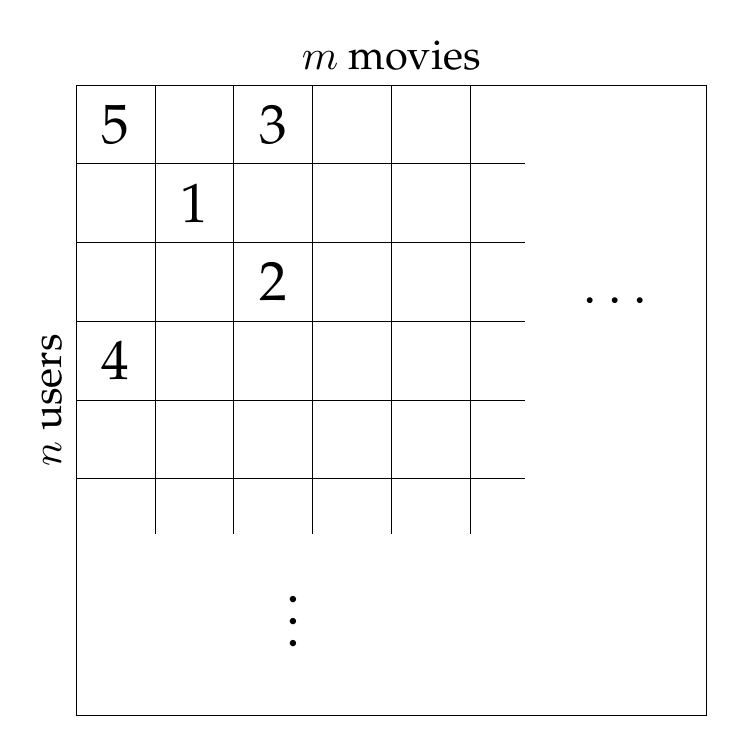
\begin{tikzpicture}
    \draw (0, 0) -- (8, 0) -- (8,-8) -- (0, -8) -- (0, 0);
    \foreach \y in {1,2,3,4,5}
      {
        \draw (0,-\y) -- (5.7,-\y);
      }
    \foreach \x in {1,2,3,4,5}
      {
        \draw (\x,0) -- (\x,-5.7);
      }
    \node[scale=2] (vdots) at (2.75, -6.6) {$\vdots$};
    \node[scale=2] (vdots) at (6.9, -2.75) {$\cdots$};

    \node[scale=2] at (0.5, -0.5) {5};
    \node[scale=2] at (2.5, -0.5) {3};
    \node[scale=2] at (1.5, -1.5) {1};
    \node[scale=2] at (2.5, -2.5) {2};
    \node[scale=2] at (0.5, -3.5) {4};
    \node[above, scale=1.5] (movies) at (4,0) {$m$ movies};
    \node[rotate=90, scale=1.5, above] (users) at (0,-4) {$n$ users};
  \end{tikzpicture}
\end{center}

$Y$ is very sparse (most entries are empty).  \note{In the Netflix
  challenge data set, there are 400,000 users and 17,000 movies.
  Only 1\% of the data matrix is filled.}  So, we will think of our
training data-set as a set of tuples $\left\{(a,i,r)\right\}$,
where $a$ is the index assigned to a particular user, $i$ is the index
assigned to a particular movie, and $r$ is user $a$'s rating of movie
$i$. We will use $D = \left\{(a,i): Y_{ai} \text{ is non-empty}\right\}$
as the set of indices for which we have a rating.

We are going to try to find a way to use $D$ to predict values for
missing entries. Let $X$ be our predicted matrix of ratings.  Now, we
need to find a loss function that relates $X$ and $Y$, so that we can
try to optimize it to find a good predictive model.

\paragraph*{Idea \#1}
Following along with our previous approaches to designing loss
functions, we might want to say that our predictions $X_{ai}$ should
agree with our data $Y_{ai}$, and then add some regularization,
yielding loss function
\[\text{Loss}\text{}(X, Y) = \frac{1}{2} \sum_{(a,i) \in D}
  (X_{ai}-Y_{ai})^2 + \sum_{\text{all } (a,i)}X_{ai}^2\;\;.\]
{\em This is a {\bf bad} idea!}  It will set $X_{ai} = 0$ for all $(a,
  i) \not \in D$.
\question{Convince yourself of that!}
We need to find a different kind of regularization that will force
some generalization to unseen entries.

\begin{examplebox}
  \paragraph*{Linear algebra idea:}
  The \emph{rank} of a matrix is the maximum number of linearly independent
  rows in the matrix (which is equal to the maximum number of linearly
  independent columns in the matrix).

  If an $n \times m$ matrix $X$ is rank 1, then there exist $U$ and $V$ of
  shapes $n \times 1$ and $m \times 1$, respectively, such that
  \[X = UV^T\;\;.\]
  If $X$ is rank $k$, then there exist $U$ and $V$ of shape $n \times k$
  and $m \times k$, respectively, such that
  \[X = UV^T\;\;.\]
\end{examplebox}

\paragraph*{Idea \#2}
Find the rank 1 matrix $X$ that fits the entries in $Y$ as well as
possible.   This is a much lower-dimensional representation (it has $m
  + n$ parameters rather than $m \cdot n$ parameters) and the same
parameter is shared among many predictions, so it seems like it might
have better generalization properties than our previous idea.

So, we would need to find vectors $U$ and $V$ such that
\[
  UV^T
  =
  \begin{bmatrix}
    \ex{U}{1} \\ \vdots \\ \ex{U}{n}
  \end{bmatrix}
  \begin{bmatrix}
    \ex{V}{1} & \cdots & \ex{V}{m}
  \end{bmatrix}
  =
  \begin{bmatrix}
    \ex{U}{1}\ex{V}{1} & \cdots & \ex{U}{1}\ex{V}{m} \\
    \vdots             & \ddots & \vdots             \\
    \ex{U}{n}\ex{V}{1} & \cdots & \ex{U}{n}\ex{V}{m} \\
  \end{bmatrix}
  =
  X \;\;.
\]
And, since we're using squared loss, our objective function would be
\[
  J(U,V) = \frac{1}{2}
  \sum_{(a,i)\in D}(\ex{U}{a}\ex{V}{i} - Y_{ai})^2 \;\;.
\]

Now, how can we find the optimal values of $U$ and $V$?  We could take
inspiration from our work on linear regression and see what the
gradients of $J$ are with respect to the parameters in $U$ and $V$.
For example,
\[
  \frac{\partial J}{\partial \ex{U}{a}} = \sum_{\{i \mid (a,i) \in D\}}
  (\ex{U}{a}\ex{V}{i} - Y_{ai})\ex{V}{i} \;\;.
\]
We could get an equation like this for each parameter $\ex{U}{a}$ or
$\ex{V}{i}$.  We don't know how to get an immediate analytic solution
to this set of equations because the parameters $U$ and $V$ are
multiplied by one another in the predictions, so the model does not
have a linear dependence on the parameters.  We could approach this
problem using gradient descent, though, and we'll do that with a
related model in the next section.

But, before we talk about optimization, let's think about the
expressiveness of this model.  It has one parameter per user (the
elements of $U$) and one parameter per movie (the elements of $V$),
and the predicted rating is the product of these two.  It can really
represent only each user's general enthusiasm and each movie's general
popularity, and predict the user's rating of the movie to be the
product of these values.
\question{
  What if we had two users, 1 and 2,  and two movies, A and B.  Can  you
  find $U, V$ that represents the data set $(1, A, 1), (1, B, 5),
    (2, A, 5), (2, B, 1)$ well?
}

\paragraph*{Idea \#3}
If using a rank 1 decomposition of the matrix is not expressive
enough, maybe we can try a {\em rank $k$} decomposition!   In this
case, we would try to find an  $n\times k$
matrix $U$ and an $m \times k$ matrix $V$ that minimize
\[J(U,V) = \frac{1}{2} \sum_{(a,i)\in D} (\ex{U}{a} \cdot \ex{V}{i}
  - Y_{ai})^2\;\;.\]

\begin{center}
  \begin{tikzpicture}[scale=1.3]
    \draw [thick] (-0.3,0) to [square left brace] (-0.3,4);
    \draw [thick] (0.7,0) to [square right brace] (0.7,4);
    \node [scale=1.6] at (0.2, 2) {$U$};

    \draw [thick] (2,0) to [square left brace] (2,4);
    \draw [thick] (6,0) to [square right brace] (6,4);

    \draw [thick] (2,4.7) to [square left brace] (2,6.2);
    \draw [thick] (6,4.7) to [square right brace] (6,6.2);
    \node [scale=1.6] at (4, 5.45) {$V^T$};

    \draw[ultra thick, blue] (-0.6, 3) rectangle (1, 3.5);
    \draw[ultra thick, red] (5, 4.7) rectangle (5.5, 6.2);
    \draw[ultra thick] (5, 3) rectangle node
      [yshift=-5ex, xshift=-2ex, scale=1.2]
      {$X_{ai} = \ex{U}{a} \cdot \ex{V}{i}$}(5.5, 3.5);
    \node [scale=1.2, left] at (-0.5, 3.25) {$\ex{U}{a}$};
    \node [scale=1.2, above] at (5.25, 6.2) {$\ex{V}{i}$};
    \draw [dotted, thick, blue] (1.2, 3.25) -- (4.8, 3.25);
    \draw [dotted, thick, red] (5.25, 4.5) -- (5.25, 3.7);
  \end{tikzpicture}
\end{center}


Here, the length $k$ vector $\ex{U}{a}$ is the $a^{th}$ row of $U$,
and represents the $k$ ``features'' of person $a$. Likewise, the
length $k$ vector $\ex{V}{i}$ is the $i^{th}$ row of $V$, and
represents the $k$ ``features'' of movie $i$. Performing the matrix
multiplication $X = UV^T$, we see what the prediction for person
$a$ and movie $i$ is $X_{ai} = \ex{U}{a} \cdot \ex{V}{i}$.

The total number of parameters that we have is $nk + mk$. But, it is
a redundant representation. We have 1 extra scaling parameter when
$k=1$, and $k^2$ extra parameters in general. So, we really effectively have
$nk + mk - k^2$ ``degrees of freedom.''
\question{Imagine $k = 3$.  If we were to take the matrix $U$ and
multiply the first column by 2, the second column by 3 and the third
column by 4, to make a new matrix $U'$, what would we have  to do to
$V$ to get a $V'$ so that $U'{V'}^T = UV^T$?  How does this question
relate to the comments above about redundancy?}

It is still useful to add offsets to our predictions, so we will
include an $n \times 1$ vector $b_U$ and an $m \times 1$ vector $b_V$
of offset parameters, and perform regularization on the parameters in
$U$ and $V$.  So our final objective becomes
\[
  J(U,V) = \frac{1}{2} \sum_{(a,i)\in D}
  (\ex{U}{a} \cdot \ex{V}{i} + \ex{b_U}{a} + \ex{b_V}{i}
  - Y_{ai})^2
  + \frac{\lambda}{2} \sum_{a=1}^n \norm{\ex{U}{a}}^2
  + \frac{\lambda}{2} \sum_{i=1}^m \norm{\ex{V}{i}}^2
  \;\;.\]
\question{What would be an informal interpretation of $\ex{b_U}{a}$?
  Of $\ex{b_V}{i}$?}

\subsection{Optimization}
Now that we have an objective, it's  time to optimize!  There are two
reasonable approaches to finding $U$, $V$, $b_U$, and $b_V$ that
optimize this objective:  alternating least squares (ALS), which builds on
our analytical solution approach for linear regression, and
stochastic gradient descent (SGD), which we have used in the context
of neural networks and other models.

\subsubsection{Alternating least squares}
One interesting thing to notice is that, if we were to fix $U$ and
$b_U$, then finding the minimizing $V$ and $b_V$ is a linear
regression problem that we already know how to solve.  The same is
true if we were to fix $V$ and $b_V$, and seek $U$ and $b_U$.
So, we will consider an algorithm that takes alternating steps of this
form:  we fix $U, b_U$, initially randomly, find the best $V, b_V$;
then fix those and find the best $U, b_U$, etc.

This is a kind of optimization sometimes called ``coordinate
descent,''  because we only improve the model in one (or, in this
case, a set of) coordinates of the parameter space at a time.
Generally, coordinate descent has similar kinds of convergence
properties as gradient descent, and it cannot guarantee that we find a
global optimum.  It is an appealing choice in this problem because we
know how to directly move to the optimal values of one set of
coordinates given that the other is fixed.

\vspace*{0.3cm}
\noindent More concretely, we:
\begin{enumerate}
  \item Initialize $V$ and $b_V$ at random
  \item For each $a$ in $1, 2, \ldots, n$:
        \begin{itemize}
          \item Construct a linear regression problem to find $\ex{U}{a}$ and $\ex{b_U}{a}$
                to minimize
                \[\frac{1}{2}\sum_{\{i \mid (a,i) \in D\}}
                  \left(\ex{U}{a}\cdot \ex{V}{i} + \ex{b_U}{a} + \ex{b_V}{i}
                  - Y_{ai}\right)^2 + \frac{\lambda}{2}\norm{\ex{U}{a}}^2
                  \;\;.\]
          \item Recall minimizing the least squares objective (we are
                ignoring the offset and regularizer in the following so you
                can see the basic idea):
                \[(W\theta - T)^T(W\theta - T)\;\;.\]
                In this scenario,
                \begin{itemize}
                  \item $\theta = \ex{U}{a}$ is the $k \times 1$ parameter
                        vector that we are trying to find,
                  \item $T$ is a $m_a \times 1$ vector of target values
                        (for the $m_a$ movies $a$ has rated), and
                  \item  $W$ is the $m_a \times k$ matrix whose rows are the $\ex{V}{i}$
                        where $a$ has rated movie $i$.
                \end{itemize}
                The solution to the least squares problem using ridge
                regression is our new  $\ex{U}{a}$ and $\ex{b_U}{a}$.
        \end{itemize}
  \item For each $i$ in $1, 2, \ldots, m$
        \begin{itemize}
          \item Construct a linear regression problem to find $\ex{V}{i}$
                and $\ex{b_V}{i}$
                to minimize
                \[\frac{1}{2}\sum_{\{a \mid (a,i) \in D\}}
                  \left(\ex{U}{a}\cdot \ex{V}{i} + \ex{b_U}{a} + \ex{b_V}{i}
                  - Y_{ai}\right)^2 + \frac{\lambda}{2}\norm{\ex{V}{i}}^2
                \]
          \item Now, $\theta = \ex{V}{i}$ is a $k \times 1$
                parameter vector, $T$ is a $n_i \times 1$ target vector
                (for the $n_i$ users that have rated movie $i$), and $W$ is
                the $n_i \times k$ matrix whose rows are the $\ex{U}{a}$
                where $i$ has been rated by user $a$.

                Again, we solve using ridge regression for a new value of
                $\ex{V}{i}$ and $\ex{b_V}{i}$.
        \end{itemize}
  \item Alternate between steps 2 and 3, optimizing $U$ and $V$, and
        stop after a fixed number of iterations or when the difference
        between successive parameter estimates is small.
\end{enumerate}

\subsubsection{Stochastic  gradient descent}
Finally, we can approach this problem using stochastic gradient
descent.  It's easier to think about if we reorganize the objective
function to be
\[
  J(U,V) = \frac{1}{2} \sum_{(a,i)\in D} \left(\left(
  \ex{U}{a} \cdot \ex{V}{i} + \ex{b_U}{a} + \ex{b_V}{i}
  - Y_{ai}\right)^2
  + \ex{\lambda_U}{a} \norm{\ex{U}{a}}^2
  + \ex{\lambda_V}{i}\norm{\ex{V}{i}}^2 \right)
\]
where
\begin{align*}
  \ex{\lambda_U}{a} & = \frac{\lambda}{\# \text{ times }(a, \_) \in D}
  = \frac{\lambda}{\sum_{\{i \mid (a,i) \in D\}} 1}                     \\
  \ex{\lambda_V}{i} & = \frac{\lambda}{\# \text{ times } (\_, i) \in D}
  = \frac{\lambda}{\sum_{\{a \mid (a,i) \in D\}} 1}
\end{align*}
Then,
\begin{align*}
  \frac{\partial J(U,V)}{\partial \ex{U}{a}}
   & = \sum_{\{i \mid (a,i) \in D\}}
  \left[\left(\ex{U}{a} \cdot \ex{V}{i} + \ex{b_U}{a}
    + \ex{b_V}{i} - Y_{ai}\right) \ex{V}{i}
  + \ex{\lambda_U}{a}\ex{U}{a}\right] \\
  \frac{\partial J(U,V)}{\partial \ex{b_U}{a}}
   & = \sum_{\{i \mid (a,i) \in D\}}
  \left( \ex{U}{a} \cdot \ex{V}{i} + \ex{b_U}{a} + \ex{b_V}{i}
  - Y_{ai}\right)
\end{align*}
We can similarly obtain gradients with respect to $\ex{V}{i}$ and
$\ex{b_V}{i}$.

Then, to do gradient descent, we draw an example $(a, i, Y_{ai})$ from
$D$ at random, and do gradient updates on $\ex{U}{a}$, $\ex{b_U}{a}$,
$\ex{V}{i}$, and $\ex{b_V}{i}$.
\question{Why don't we update the other parameters, such as
  $\ex{U}{a'}$ for some other user $a'$ or $\ex{V}{i'}$ for some other
  movie $i'$?}


%%% Local Variables:
%%% mode: latex
%%% TeX-master: "top"
%%% End:

%\section{Collaborative filtering and the SVD}
\label{app:collab_filter}

~\\

This appendix presents the relationship between collaborative filtering
and the singular value decomposition, a fundamental matrix
decomposition method in linear algebra.

Recall that the goal of collaborative filtering is to approximate an
$n\times m$ matrix $Y$ into a rank $k$ matrix $X$, where $X$ is decomposed as the product of an $n\times k$ matrix $U$,
and a $k\times m$ matrix $V^T$, i.e., $X = UV^T$.  Let us denote the
$k$ {\em columns} of $U$ as $\{u_i\}$ (for $i$ in $1\cdots k$), and
the $k$ {\em rows} of $V^T$ as $\{v_i\}$.  This decomposition may be
visualized as the following matrix product:

% \setlength{\extrarowheight}{1ex}
\newcommand*{\vertbar}{\rule[-1ex]{0.5pt}{2.5ex}}
\newcommand*{\horzbar}{\rule[.5ex]{2.5ex}{0.5pt}}

\begin{eqnarray}
X = U V^T = 
\left[
  \begin{array}{cccc}
    \vertbar & \vertbar &        & \vertbar \\
    u_{1}    & u_{2}    & \ldots & u_{k}    \\
    \vertbar & \vertbar &        & \vertbar 
  \end{array}
\right]
\left[
  \begin{array}{ccc}
    \horzbar & v_{1} & \horzbar \\
    \horzbar & v_{2} & \horzbar \\
             & \vdots    &          \\
    \horzbar & v_{k} & \horzbar
  \end{array}
\right]
\end{eqnarray}

Recall that $k$ is the rank of $X$, and thus each $u_i$ is linearly
independent of all other column vectors of $U$, and similarly for
$v_i$.  (This makes the $k$ features independent of each other.)
Because of this linear independence, we may choose $u_i$ such that
$(u_i)^T u_j = ||u_i||^2 \delta_{ij}$ is zero for $i\neq j$, meaning
that each $u_i$ is {\em orthogonal} to other column vectors of $U$.
This orthogonalization can be done using a Gram-Schmidt process, for
example.  The row vectors $v_i$ can similarly be constructed to be
orthogonal, and in the following we assume the $\{u_i\}$ and $\{v_i\}$ are
each sets of orthogonal vectors.

Consider, now, what happens when the $n\times m$ matrix $X$ is left-multiplied by one of the $1\times n$ vectors $(u_i)^T$.  Evidently
\begin{eqnarray}
(u_i)^T X = \sum_j (u_i)^T u_j v_j = ||u_i||^2 v_i
\,,
\end{eqnarray}
where $||u_i||^2$ is the square of the norm of the vector $u_i$.  Similarly, when $X$ is right-multiplied by one of the $m\times 1$ vectors $(v_i)^T$, we get:
\begin{eqnarray}
X (v_i)^T = \sum_j u_j v_j (v_i)^T = ||v_i||^2 u_i
\,.
\end{eqnarray}
Combining these to compute the right-multiplication of $X^TX$ by $(v_i)^T$, we observe something very interesting:
\begin{eqnarray}
X^T X (v_i)^T =  ||v_i||^2 X^T u_i = ||v_i||^2 ( (u_i)^T X )^T = ||v_i||^2  ||u_i||^2  (v_i)^T
\,,
\end{eqnarray}
which means that $(v_i)^T$ is a ``right'' {\em eigenvector} of $X^T X$, with eigenvalue $||v_i||^2 ||u_i||^2$!  Similarly, the
left-multiplication of $XX^T$ by $(u_i)^T$ gives:
\begin{eqnarray}
(u_i)^T X X^T = ||u_i||^2 v_i X^T = ||u_i||^2  ( X (v_i)^T )^T = ||u_i||^2  ||v_i||^2  (u_i)^T
\,,
\end{eqnarray}
which means that $(u_i)^T$ is a ``left'' eigenvector of $XX^T$, with eigenvalue $||u_i||^2 ||v_i||^2$.

How many eigenvectors do we have?  Well, $X^T X$ is an $m\times m$
positive-definite matrix, so it must have $m$ eigenvectors; let us
thus extend our definition of $\{v_i\}$ to be all these $m$
eigenvectors.  And $XX^T$ is an $n\times n$ positive-definite matrix,
which has $n$ eigenvectors, so let us similarly extend our definition
of $\{u_i\}$.

Eigenvectors provide orthogonal bases for linear vector spaces, and thus it is convenient to normalize them.  Let us define
\begin{eqnarray}
  \tilde{u}_i &=& \frac{u_i}{||u_i||}
  \\
  \tilde{v}_i &=& \frac{v_i}{||v_i||}
\end{eqnarray}
as the columns of matrix $\tilde{U}$ and the rows of matrix
$\tilde{V}^T$.  Let us also define the diagonal matrix $\Lambda_{ii} = ||u_i|| ||v_i||$.  
Using these newly defined matrices, we may now rewrite $X$ as
\begin{eqnarray}
  X = UV^T =\tilde{U} \Lambda \tilde{V}^T
  \,,
\end{eqnarray}
where, to summarize, the $n\times n$ matrix $\tilde{U}$ has as its
columns the normalized left-eigenvectors of $XX^T$, the $m\times m$ 
matrix $\tilde{V}$ has as its rows the normalized
right-eigenvectors of $X^TX$, and $\Lambda$ is a diagonal matrix of
the products of the square roots of the eigenvalues.

This is known as the {\em singular value decomposition} of $X$!  The
SVD is a standard matrix decomposition, and the diagonal elements of
$\Lambda$ are known as the {\em singular values} of $X$.  These
singular values are non-negative, real values, and thus $\Lambda$ may
be viewed as a scaling matrix.  Meanwhile, $\tilde{U}$ and $\tilde{V}^T$ geometrically
act as rotation matrices, because they are {\em unitary} matrices:
$\tilde{U}^T \tilde{U} = I$ and similarly for $\tilde{V}^T$.

How does this relate to the collaborative filtering decomposition,
where $U$ and $V$ are not square matrices?  Well, the largest singular
values of $Y$ contribute ``most'' to $Y$, and thus an important method
of approximating $Y$ to some degree $k$ is to compute $Y' = \tilde{U}
\Lambda' \tilde{V}^T$, where $\Lambda'$ only keeps the $k$ largest
singular values, and drops the rest to zero.  We may also drop rows of
$\tilde{V}^T$ and columns of $\tilde{U}$ corresponding to the dropped
singular values, producing rank-$k$ matrices $U$ and $V$.  This is
known as taking the rank $k$ {\em principal component} of $Y$,
providing $Y'$ which has the smallest possible Frobenius norm with
$Y$, i.e., minimizing the square root of the sum of the absolute square
of the elements of $Y-Y'$.

This shows how singular value decomposition is mathematically related
to collaborative filtering, but how do they compare algorithmically?
In practice, $Y$ may have missing (or hidden) entries, and standard
techniques for computing the SVD may not be robust against such
missing data.  Computing full sets of eigenvectors and eigenvalues can
also be computationally expensive, especially if you only want those
corresponding to the largest $k$ singular values.  Thus, there can be
advantages to collaborative filtering algorithms, e.g., those based on
gradient descent, although modifications can also be made to improve
the robustness of the SVD approach.




\end{document}